
%%\documentstyle[11pt,epsf]{report}
\documentclass[11pt]{report}
\usepackage{epsf}
\usepackage{epsfig}
\usepackage{amsthm}

\pagestyle{headings}

% LaTeX Size Stuff
%-----------------
\setlength{\topmargin}{-0.25in}
\setlength{\headheight}{10pt}
\setlength{\headsep}{30pt}
\setlength{\oddsidemargin}{0.0in}
\setlength{\evensidemargin}{0.0in}
\setlength{\textheight}{8.5in}
\setlength{\textwidth}{6.5in}
\setlength{\footskip}{50pt}
%\setlength{\footheight}{24pt}
\setlength{\parskip}{4mm}               % space between paragraphs

\def\cut{\mbox{\tt '!'/0}}
\def\not{\mbox{${\tt '\backslash+'/1}$}}
\def\sldnf{\mbox{${\tt \backslash+}$}}

\newcommand{\ourprolog}{XSB}
\newcommand{\smallourprolog}{xsb}
\newcommand{\version}{Version 1.4.2}

%%\newcommand{\qed}{\mbox{$\ \Box$}}
\newcommand{\lqed}{\qed\vspace{.1in}}
\newcommand{\nf}{\mbox{$\sim$}}
\newcommand{\wt}{\mbox{$\widehat{T}$}}
\newcommand{\as}{\mbox{$/\hspace{-2mm}>$}}
\newcommand{\equi}{\mbox{$\leftrightarrow$}}
\newcommand{\myeq}{\mbox{$\leftrightarrow$}}
\newcommand{\myra}{\mbox{$\Rightarrow$}}
\newcommand{\tab}{\hspace*{4em}}
\newcommand{\ind}{\hspace*{2em}}
\newcommand{\longline}{\noindent\rule{\textwidth}{.01in}}

\newcommand{\bg}{\hspace*{.7cm}}
\newcommand{\s}{\hspace*{.3cm}}

\newcommand{\demo}[1]{\hspace*{1.5cm}{\tt #1}}
\newcommand{\desc}[1]{\item[{\tt #1}]\hspace*{1mm}\newline}
\newcommand{\desce}[1]{\item[{\tt #1}]}
\newcommand{\ouritem}[1]{\item[{\mbox{\tt #1}}]\ \\}
\newcommand{\ournewitem}[2]{\item[{\mbox{\tt #1}}]\hspace*{\fill}{\mbox{\sf #2}}\ \\}

\newtheorem{example}{Example}[section]
\newtheorem{proposition}{Proposition}[section]
\newtheorem{theorem}{Theorem}
%%\newtheorem{proof}{Proof}

\newcommand{\stuff}[1]{
        \begin{minipage}{4in}
        {\tt \samepage
        \begin{tabbing}
        \hspace{8mm} \= \hspace{6mm} \= \hspace{10mm} \= \hspace{55mm} \= \kill
        #1 \hfill
        \end{tabbing}
        }
        \end{minipage}
}
\newtheorem{dummylemma}{Dummy}[section]
\newtheorem{DefinitioN}[dummylemma]{\bf Definition}%[section]
\newenvironment{definition}[1]
               {\begin{DefinitioN}\rm {\bf (#1)}}{\hspace{1cm} \hfill \end{DefinitioN}}

%------------------------------------------------------------
%\input{predind.sty}
%\makepredindex
%\makeindex
%------------------------------------------------------------

\begin{document}

\title{\bf Programming in Tabled Prolog \\ (very) DRAFT
\footnote{This is a very early draft made available privately for
those who might find it of interest.  I reserve all rights to this
work. -dsw}
}

\author{% {\epsfxsize=230pt \epsfbox{xsb-logo.eps}}\\
        \ \\ \ \\
        {\em David S. Warren} \\ 
        \ \\
        {Department of Computer Science} \\
        {SUNY @ Stony Brook} \\
        {Stony Brook, NY 11794-4400, U.S.A.} \\
        \ \\
} 

\date{\today}

\maketitle

\bibliographystyle{plain}

\thispagestyle{empty}
%\input{ack}
\newpage

\pagenumbering{roman}
\tableofcontents
\newpage        % Just to avoid a silly LaTeX bug with \pagenumbering
  
\pagenumbering{arabic}

\chapter{Background and Motivation: Why Tabling?}

There is a flaw in the very foundations of Logic Programming: Prolog
is nondeclarative.  Of course, everyone knows that real Prolog as it
is used is nondeclarative.  Prolog programs abound with cuts, var
tests, asserts, and all kinds of ugly warts.  Everyone agrees that
Prolog should be more declarative and much research time has been
spent, and spent productively, trying to remedy these problems by
providing more declarative alternatives.  But I believe that there is
a more serious flaw closer to the heart of Prolog, right at its very
center, and this flaw has caused a number of problems in logic
programming.  I'm convinced that we must address this flaw, before we
can proceed together productively with logic programming.  Of course,
whether this is a ``flaw'' is in the eye of the beholder; we all have
arguments over whether a particular behavior is a bug or a feature.
As is clear from my presentation, I think I've found a bug; some of
you will think it's a feature.  Wherever we stand on this issue,
however, I believe we must be clear about its implications.  Only then
will we be able to communicate effectively about where LP is and where
it should go.

Let me also mention that I am by no means pointing out something new,
unknown to the community; rather I'm trying to raise our consciousness
about an inconsistency and its implications.

The problem is the very semantics of logic programming.  The
foundational results of our field show that for pure horn clauses, the
following are equivalent: logical implication, SLD resolution, and the
least fixpoint of the $T_p$ operator.  And logic programming basically
``works'' because SLD corresponds to computation (i.e. Prolog) {\em
and} to logical implication (truth in models).

But there is a fly in the ointment, the dirty secret that we Prolog
aficionados try to keep in the closet but Prolog programmers are all
too aware of.  Let's look more carefully at the full SLD tree, the
foundation for us Prolog hackers.  There are three kinds of paths in
an SLD tree: 1) those ending in success, 2) those ending in failure,
and 3) those not ending.  The foundational results tell us that those
ending in success correspond exactly to those instances of the query
that logically follow from the program.  This is fine and dandy and
certainly something we want and need.  But as programmers, that's not
enough.  We programmers also want, need actually, to distinguish
between paths that end in failure and paths that don't end at all.
When we run a program, and it responds `no', we may accept that
response as a good answer to our query.  But if it goes into an
infinite loop never coming back with an answer at all, we decide we
have a bug in our program and set out to fix it.  

So the problem with SLD is not that it doesn't do the right things for
success, but that it doesn't do the right thing with the other two
possible outcomes.  Note that this has nothing to do with how we
search the SLD tree, e.g. unfairly with depth first search or fairly
with breadth-first search; it's a property of the tree itself.  And it
has nothing to do with the fact that our theory deals best with ground
programs and Prolog programs deal with variables.  The problem
concerns which paths in the SLD tree are finite and which are
infinite.

In Prolog, as compared with other languages, it seems easier to write
partially correct programs, programs that, if they halt, they give the
right answers.  This comes from the power of declarative programming.
But it seems much harder to write and reason about totally correct
programs, programs that halt in all (the right) cases.  So it may be
the case that what we gain from declarativeness in our ability to
reason about the partial correctness of Prolog programs, we lose in
the difficulty of reasoning about total correctness.  Theoreticians
may accept partial correctness as good enough; but we users have to
know precisely how partial.

And sadly, the problems show up for very simple programs.  The issue
is clearly seen in transitive closure.  Consider the definition:

\begin{verbatim}
tca(X,Y) :- a(X,Y).
tca(X,Y) :- a(X,Z), tca(Z,Y).
\end{verbatim}

Prolog programmers know that this definition is fine when the
predicate ``a'' stands for ``parent'', and then ``tca'' is
``ancestor''.  But what happens if ``a'' is defined by the following
facts?

\begin{verbatim}
a(1,1).
a(2,1).
\end{verbatim}

Consider what happens when we ask the query: :- tca(1,2).  Prolog (that
is SLD resolution) goes into an infinite loop.  Are we as programmers
happy?  Do we say that since it hasn't returned, it must mean that you
can't get to 2 from 1 in this graph?  Not at all.  We turn back to fix
the program, probably modifying it by adding a loop-check.  That is,
we add a list of nodes to the predicate ``tca'', which contains the
nodes already visited.  Then before continuing to search from a node,
we check that it has not already been visited.  We're not happy until
our program responds `no' to our query.  So clearly the semantics of
our programming language is going to have to account for this.  And it
does.  We can't depend on the previously referenced foundational
results to give a semantics for pure Prolog as a programming language,
where we want to know what both `yes' and `no' answers mean.  The
theory must somehow be extended.  This was done in \cite{} by Kenneth Clark who defined
the completion of a program.  The semantics of (pure) Prolog programs
is normally taken to be the logical implications of the completion
(plus some standard axioms such as the unique names axiom.)  To find
the completion of our tca/2 program, we first convert the two
implication rules for tca/2 into the equivalent one implication with a
disjunction in the antecedent, and then we turn the implication into a
biconditional.  We do a similar transformation for a/2.  Then we take
the meaning of the program to be the logical implications of these
biconditionals (including some standard axioms).  And it is the case
that $\sim tca(1,2)$ is not logically implied by this theory (and
neither is tca(1,2), of course.)  So the completion semantics correctly
tells us that SLD will not terminate for this query.  And indeed
Prolog theoreticians (as well as the programmers) know that tca/2 as
defined above is NOT a general definition for transitive closure.
(But note that it {\em is} transitive closure if the graph is acyclic.
Maybe this is OK, since it is often the case that algorithms for
constrained data are simpler, but here it could be rather confusing, I
think.)

But in any case the Prolog community was (mostly) happy with this
situation, until the database people showed up and asked the obvious
question: Why doesn't the obvious two-line definition of tca/2 indeed
mean transitive closure?  (To some of us, it felt somewhat as though
they were pointing out that the emperor had no clothes.)  They pointed
out that if one uses the fixed point characterization from the
original foundation trilogy, instead of the SLD characterization, it
does.  Indeed, transitive closure is only the beginning; there are
many advantages in using this semantics.  {\em All} programs without
function symbols are terminating, and many simple programs now have a
natural programmers' semantics.  Indeed DCG's now {\em do} mean the
corresponding context free languages, whereas under the completion
semantics they don't always.  But even more important is what this
fixpoint semantics does to the theory of programs.  The theory is much
simpler, and accords with theory already developed.  E.g., automata
theory (e.g. CFL's) is now correctly reflected in LP.  And also
interestingly, this semantics leads the way for a theory of default
negation, which has blossomed.  This is because if we have a better
idea of when things are known false, the theory describing such
negative knowledge is simpler, more interesting, and perhaps even more
useful.

Actually, the situation for the completion is somewhat worse than
implied by the transitive closure example.  There are programs for
which Prolog goes into an infinite loop even though the completion of
the program determines all goals.  And this is {\em not} because
Prolog is depth-first; it's because its selection rule is
left-to-right.  To get Prolog actually to display the behavior
predicted by the completion, one would have to interleave computations
of all goal orderings, and fail a goal if any of the interleavings
failed.  This is hardly an attractive alternative for Prolog
implementors or programmers.

So I personally think minimal model semantics (i.e., the fixpoint
semantics) is better than the completion semantics for logic
programming.  I think the completion semantics is a bug, which should
be fixed, and it should be fixed by taking the fixpoint semantics.
There are those who either don't think this is a bug, or don't think
that this is a reasonable fix.  I certainly accept that the point is
arguable.  Going to the fixpoint semantics is a big step for at least
two reasons: 

\begin{itemize}
\item[Objection 1:] 
It violates a principle dear to the hearts of some theoretically
inclined logic programmers, that the meaning of a program consists of
the logical implications of the theory of the formulas making up the
program (or a simple transformation of them).

\item[Objection 2:]
It violates a principle dear to the hearts of some practically
inclined logic programmers (like me), that a program should have the
well-known procedural semantics, i.e., be executable by SLD resolution
(and WAM engines).

\end{itemize} 

The first objection is real and in some sense is not satisfactorily
solvable, I believe.  We know that there is no first-order theory that
characterizes transitive closure (the usual Prolog loop-check program
requires default negation.)  I will discuss some implications of this
later, and try to claim that things aren't so bad, but I can't say
they aren't true.  Basically, the purpose of this entire book is to
claim that the second objection can be overcome.  It is overcome by
using OLDT resolution \cite{} (or a generalizaiton SLG Resolution \cite{})
in place of SLD resolution in the foundational
theorems.  OLDT is a resolution strategy very similar to SLD, but one
that avoids redundant computation by remembering subcomputations and
reusing their results to respond to later requests.  This remembering
and reuse has been called memoization, tabling, lemmatization,
caching, well-formed substring tables, and probably a number of other
names.  With OLDT instead of SLD, the foundational theorem can be even
stronger, including a theorem relating OLDT failure leaves and the
fixpoint definition.

OLDT terminates (i.e., has only success and failure leaf nodes) for
all queries to programs that have finite minimal models, i.e. that
have a least fixpoint of finite size.  This guarantees total
correctness for the transitive closure definition (over finite
graphs).  Actually, even more can be said: OLDT terminates for all
queries to programs for which only a finite portion of the minimal
model is looked at; that is, for all programs with the Bounded Term
Size (BTS) property.  BTS is slightly circular, and undecidable, but
to me intuitively says that any finitary, constructive definition will
terminate.  (Admittedly, this is also somewhat circular.)

One thing that happens when we do not have first-order theories to
explain our semantics, i.e. the first objection above, is that we may
leave the realm of recursively enumerable sets.  That is, if we did have a first-order
theory to explain the semantics, then we'd know that a theorem-prover
could enumerate the theorems and the semantics would be r.e.  However,
by going to the minimal model semantics, we may (and do, when we add
negation) get non-r.e.~sets.  That is, we leave the realm of the
computable sets.  This might give pause to someone interested in
computation, because then we can write programs that aren't in
principle computable.  Note that this isn't a problem for totally
correct programs (which will be recursive programs), which are those
we usually want to write.  I guess that just as we rely on the
programmer to write programs that are terminating, we must rely on the
programmer to write programs that are computable.

SLDNF was the obvious (and perhaps only reasonable) extension of SLD
to include default negation.  If we are to base our new logic
programming on OLDT, the question arises as to how OLDT should be
extended to handle negation.  Given the theory of default negation
developed over the last several years, it seems that the well-founded
semantics is the appropriate semantics to compute for logic programs
with unconstrained negation.  (The other possible semantics is the
partial stable model semantics, but this is NP complete for
propositional programs, so may be not particularly appropriate for a
basic computational mechanism.)  For OLDT there have been several
proposals for computing the well-founded semantics, in particular
WELL! and XOLDTNF, which are quite similar.  The one I'm proposing
here is SLG, which I claim is the (or a) right one.  The simplest
reason that SLG is better than the previous two is that they are
exponential for general propositional normal programs, whereas SLG is
polynomial.  Also SLG produces a residual program when there are
undefined atoms in the well-founded models, and this residual program
can be further processed to find certain partial stable models.  So in
many cases SLG could be used as a preprocessor for a partial stable
model evaluator.

SLG implements the procedural interpretation of Horn clauses, with the
addition of tabling.  This is a more complex procedural interpretation
than SLDNF (and the procedural interpretation of negation makes it
even more complex), but I think it is indeed a procedural
interpretation and I think it is acceptable.  But this is not enough
to respond fully to objection 2 above.  The Prolog programmers want to
know if SLG can be implemented so that it is efficient enough to
compete with Prolog, (or actually efficient enough to compete with
C++, perhaps our {\em true} competitor.)  I think the answer is `yes'.
Actually, even more than that, I think it will be the case that we
will be able to construct an engine that for many useful problems will
be significantly faster than Prolog.  And these problems will be in
what has historically been logic programming's core applications:
natural language, AI search, knowledge bases, and databases.
The examples in this book
will indicate in detail where some of the problems lie.  There is much
work to do, but I will claim that results we already have in the XSB
project indicate that it will definitely be possible.

The approach is to take SLG as the basic computation strategy, and to
use SLDNF as an optimization.  So when SLDNF can be proved to have the
same behavior as SLG, then we can use it and get current Prolog
speeds.  To do this we need an implementation that fully and closely
integrates SLG and SLD, allowing them to be used interchangably and
intermixedly.  And that is what SLG resolution supports and its
implementation in XSB achieves.

\chapter{Introduction to Prolog} \label{introduction}

This chapter introduces the Prolog programming language.  Here we will
explain a bit of how Prolog works.  It is not intended to be a full
description of how to become an expert Prolog programmer.  For that,
after reading this chapter, you should refer to another book, such as
{\em Programming in Prolog} by Clocksin and Mellish, or if you are
already very familiar with Prolog, you might look at {\em The Craft of
Prolog} by Richard O'Keefe.  While this is an introduction to Prolog,
even experts may find something of interest in this chapter, since I
explain Prolog in a somewhat unusual way, that may give new insights
to old Prolog programmers.

Prolog's name is short for ``Programming in Logic'' (or really for
Programmation Logique?'')  As its name suggests, Prolog is firmly
based on logic, and Prolog programs can be understood as statements in
a formal logic.  I.e., a Prolog program can be thought of as a set of
statements in first-order logic, and the meaning of the program is the
set of true implications of those logical statements.  This is the
approach that is usually taken to describe Prolog programming to
novices.  However, the amazing thing about logic programming to me is
not that it is logic, but that it is programming.  These Prolog
programs are not only statements in a logic but they are also
statements in a programming language.  This is referred to in the biz
by saying that Prolog programs have a procedural interpretation (i.e.,
as programs) as well as a declarative interpretation (i.e., as
statements in a logic.)  The introduction to Prolog that I give here
will emphasize its procedurality.  This may be anathema to some Prolog
purists (and it certainly would have been to me a while ago) but I now
feel that this is the best way to introduce logic programming to
computer scientists who already know about programming.  We will build
on your understanding of programming, and use that to lead to logic.

\section{Prolog as a Procedural Programming Language}

Prolog, as a programming language, is a little unusual.  It can be
understood as a standard procedural language with two unusual
properties.  It is a procedural language like C or Algol.  One
programs in a procedural language by writing procedures that carry out
particular operations.  One specifies what a procedure is to do by
using primitive statements and by invoking other procedures.  Prolog
procedures have only local variables and all the information that a
procedure can use or produce must be passed through its arguments.

C can be viewed as a procedural language by thinking of using it
without functions; i.e., all functions return void, and information is
passed to and from functions through their arguments only.

In Prolog, procedures are called predicates.  The two unusual aspects
of Prolog are:
\begin{enumerate}
\item Prolog has assign-once variables, and 
\item Prolog is nondeterministic.
\end{enumerate}

\subsection{Assign-once Variables}

By saying that Prolog has assign-once variables, I mean that any
particular variable in a Prolog procedure can only ever get one value
assigned to it.  A Prolog variable at any point in execution either
has a value, which can thereafter never be changed, or it has not yet
been given a value.  This may seem to be an incredibly strong
restriction.  In C, for instance, one usually programs by setting
a variable's value and then changing it during the execution of the
program.  For example, to sum up an array of numbers, one sets the
accumulator variable to 0 and the loop variable to 1, and then
increments the loop variable to step through the array modifying the
accumulator at each step.  How in the world could this be done with
assign-once variables?  The secret is that it can be done easily
through the use of recursion.

So let's write a simple Prolog program to see how we can do something
interesting with only assign-once variables.  Let's consider the
problem of adding up the numbers in a list.  Prolog is a
list-processing language, similar to Lisp.  Its primary data structure
is the tree (called a term), a very common form of which is the list.
There are three basic data types in Prolog: 1) integers, 2) floating
point numbers, and 3) atoms.  The first two should be
self-explanatory.  Atoms are simply symbols that represent themselves.
Prolog terms (trees) are constituted of integers, floats, atoms and
other terms.

A list in Prolog is written with square brackets and with its elements
separated by commas.  For example the following are lists:
\begin{verbatim}
     [1,2,3]  [aa,bbb,d]  []  [[2,b],or,not,[2,b]]
\end{verbatim}
The first is a list of integers, the second a list of atoms, the third
is the empty list consisting of no elements, and the fourth is a list
containing four elements, the first and last being themselves lists.

So let's now write a program in a made-up procedural language (that is
{\em not} Prolog, but somewhat similar) and see if we can sum up the
elements of an integer list with assign-once variables.

\begin{verbatim}
    sum(List,Sum) :-
        if List = []
          then Sum := 0
          else Head := head(List)
               Tail := tail(List)
               sum(Tail,TailSum)
               Sum := TailSum + Head
\end{verbatim}
The first line (preceding the \verb|:-|) declares the name of the
procedure and its formal parameters.  The remaining lines (following
the \verb|:-|) make up the body of the procedure definition.  We have
assumed the existence of two functions, head and tail, to extract the
first element of a list, and the remainder of the list after the head
is removed, respectively.  Sum is a recursive procedure.  It takes a
list of numbers as its first argument and returns the sum of the
numbers in its second.  It first checks to see if the list is empty.
If so, it sets the sum to 0 and returns directly.  If not, it saves
the first element of the list in a local variable, \verb|Head|, and
then calls \verb|sum| recursively on the tail of the list, getting the
sum of the rest of the list in the local variable \verb|TailSum|.  It
then adds \verb|Head| to \verb|TailSum| to get the value for
\verb|Sum|, which it sets and returns.  Notice that no single variable
gets two different values.  The variable \verb|Sum| is not set and
then changed; each recursive invocation has a different \verb|Sum|
variable and each gets set only once, to its appropriate partial sum.
Note also that the loop variable in the iterative version of summing
an array is here replaced by the variables containing each sublist.
So here too there is no need to have multiply assigned variables.
Instead of one variable getting many values, we can instead uses many
variables, each getting one value.  (Let me point out for those of you
who may be worried about efficiency that this is a conceptual point;
it may well be that the underlying implementation of such a program
would actually use just one location for all the \verb|Sum|
variables.)

So we see that we are able get by in this case
with assign-once variables.  It turns out
that this idea of using recursion and the multiple variables at the
different recursion levels is very general.  This is not just a trick
that works in this case only, but is an example of a very general
technique.

Now having assign-once variables gives rise to a very interesting
phenomenon: assignment can be symmetrical in Prolog.  That is, Prolog
doesn't have to treat the left and the right sides of an assignment
differently, as must be done in normal procedural languages such as
C or Java.  As a matter of fact, Prolog doesn't have to treat tests
and assignments differently either.  I.e., Prolog doesn't need two
operators, say == for testing and = for assignment as C does; it needs
only one.  

Let's first consider assignment.  Consider the following assignments:
\begin{verbatim}
     X := 5
     Y := X
\end{verbatim}
We'll assume that neither \verb|X| nor \verb|Y| have been assigned a
value before this sequence is executed.  So \verb|X| gets the value 5
by the first statement, and then \verb|Y| is assigned the value of
\verb|X|, so \verb|Y| gets the value 5 as well.  Now consider the
following statements:
\begin{verbatim}
     X := 5
     X := Y
\end{verbatim}
The first statement again assigns 5 to \verb|X|.  Now consider the
second.  \verb|X| has the value 5 and \verb|Y| has no value.  Since
Prolog is an assign-once language, \verb|X| can get only one value and
it already has it, so we know we can't change it.  But \verb|Y|
doesn't yet have a value.  So the only reasonable thing to do is to
set \verb|Y| to be 5, i.e., to \verb|X|'s value.  Note that this
sequence of assignments has the same net effect that the previous
sequence had.

This suggests how we can treat both sides of an assignment in the same
way.  If one of the variables has a value and the other doesn't, then
assign the value that the one has to the other.  If neither variable
has a value yet, then make it so that whenever one of them gets a
value, the other gets that same value.  If they both have a value,
then if it's the same value, then the assignment is a no-op.  If the
two values are different, then there is a problem since neither can
get a new value.  In this case we say the computation fails.  (We will
talk more about failure later.)

Notice that this definition of ``assignment'' means that any ordering
of the same (or symmetric) assignments gives the same result.  For
example, consider the different ordering of our assignments above:
\begin{verbatim}
     X := Y
     X := 5
\end{verbatim}
Again assuming that \verb|X| and \verb|Y| start with no values, the
first statement causes Prolog to bind \verb|X| and \verb|Y| together,
so that whenever one of them gets a value, the other will also get
that same value.  Then the second statement causes \verb|X| to get the
value 5, and so \verb|Y| gets that value, too.  So after these two
assignments are executed, both \verb|X| and \verb|Y| have the value 5,
exactly as they do after the previous two versions of these
assignments.  This is also a very general phenonemon: with this
meaning of assignment, any ordering of any set of assignments gives
the same result.

So let's rewrite our sum program with these ideas in mind.  We will
use = for our symmetric assignment statement.  (From now on, all our
programs will be syntactically correct Prolog, and XSB, programs, so
you can type them into XSB and try them out. [sidebar] to explain how
to create files, consult them, and run defined predicates).

\begin{verbatim}
    sum(List,Sum) :-
        List = []
         ->   Sum = 0
         ;    List = [Head|Tail],
              sum(Tail,TailSum),
              Sum is TailSum + Head.
\end{verbatim}
I've changed the syntax for if-then-else to Prolog's syntax, using
\verb|->| and \verb|;|.  Here we've said that \verb|Sum = 0|; using
the properties of symmetric assignment, we could just as well have
said that \verb|0 = Sum|.  Consider the symmetric assignment:
\verb^List = [Head|Tail]^.  The structure on the right is how one
constructs a list from a head element and a tail list.  (In Lisp it is
known as \verb|cons|.)  So our symmetric assignment here is even more
powerful.  We know that the variable \verb|List| has a list as its
value.  So this assignment assigns both variables \verb|Head| and
\verb|Tail| so that they get the values of the first element of
\verb|List| and the tail of \verb|List|, respectively.  We can see
that symmetric assignment is here extended to matching.  We match the
value in the variable \verb|List|, which is a list, to the structure
\verb^[Head|Tail]^.  \verb|Head| and \verb|Tail| are the only variables
without values, so the symmetric assignment will fill them in with the
appropriate values to make the \verb|List| and the \verb^[Head|Tail]^
structure the same.  This matching process, which we have been
referring to as ``symmetric assignment'', is called {\em unification}.

Notice that we've used the same operation of unification, 
\verb|List = []|, 
in the test of the if-then-else.  Here we see a use of failure.
Recall that we said that if a symmetric assignment cannot be made
because the two sides have values that are different, then the
assignment (or unification) fails.  The if-then-else construct does
the unification and if it succeeds, then it executes the then
statement (which follows the \verb|->|); if it fails, it executes the
else statement (which follows the \verb|;|.)  So even the boolean test
of an if-then-else can use our universal unification operation.

Notice, however, that we have not used unification for the last
statement that adds Head to the partial sum.  This is because here we
don't want to match the two sides, since Prolog considers the right
side to be a tree (with + at the root and with two leaves of TailSum
and Head.)  So here we must use an operation that explicitly asks for
the tree on the right to be evaluated as a numeric expression.  In
Prolog that operation is named \verb|is|.

As another example, consider the append procedure:
\begin{verbatim}
    append(L1,L2,L3) :-
        L1 = []
         ->  L3 = L2
         ;   L1 = [X|L1t],
             append(L1t,L2,L3t),
             L3 = [X|L3t].
\end{verbatim}
This is a procedure that takes two lists and concatenates them
together, returning the resulting list in its third argument.  This
definition says that if the first list is empty, then the result of
concatenating \verb|L1| and \verb|L2| is just \verb|L2|.  Otherwise,
we let \verb|X| be the head of the first list and \verb|L1t| be its
tail.  Then we concatenate \verb|L1|t and \verb|L2|, using append
recursively, to get \verb|L3t|.  Finally we add \verb|X| to the
beginning of \verb|L3t| to construct the final result, \verb|L3|.

Consider the following version of append:
\begin{verbatim}
    append(L1,L2,L3) :-
        L1 = [X|L1t]
         ->  L3 = [X|L3t],
             append(L1t,L2,L3t)
         ;   L3 = L2
\end{verbatim}
This one looks rather strange, but it also works.  We've used the
boolean test unification also to deconstruct the list.  (This is
probably a poor idea in real Prolog programming.)  The other perhaps
stranger (but less bad) difference is that we've moved the
construction of the output list \verb|L3| to before the recursive call
to \verb|append|.  You might wonder how we can construct a list before
we have its components.  But with unification, that works just fine.
The intuition is that if a variable can get only one value, it doesn't
really matter when it gets it.  So it is often the case that
unifications can be moved earlier.  What happens here is that the list
cell is constructed before the call to \verb|append|, and then the
recursive call to \verb|append| will fill in the tail of that cell
with the appropriate value.

We've looked at assign-once variables and seen how they lead to
symmetric assignment, which leads to unification.  Next let's consider
the other unusal property of Prolog programs, the fact that they can
be nondeterministic.

\subsection{Nondeterminism}

C is a deterministic programming language (as are Java and most any other language you ar familiar with);
at any point in the execution of a C program there is exactly one
next step, which seems reasonable since the machines we execute these programs on are (essentially) deterministic.  
Prolog, however, is nondeterministic.  There are points in
the execution of a Prolog program when there are multiple legal next
steps.  The way this is specified in Prolog is to give multiple
definitions of the same procedure.  For example, we could write a
procedure to find both square roots of a positive real number by:
\begin{verbatim}
    a_sqrt(X,Y) :-
        X > 0,
        Y is sqrt(X).
    a_sqrt(X,Y) :-
        X > 0,
        Y is -sqrt(X).
\end{verbatim}
\verb|a_sqrt| takes a number and returns its square root.  Here we want it
to return both square roots, one positive and one negative.  We can do
that by giving two definitions of a procedure \verb|a_sqrt|.  A C
compiler would complain that the procedure is multiply defined, but
Prolog accepts such multiple procedure definitions happily.  The first
definition checks that the input argument is greater than 0, and if so
uses a Prolog primitive builtin to calculate the positive square root.
The second definition does the same, but returns the negation of the
positive square root.  In Prolog terminology, each definition is
called a ``clause'', so \verb|a_sqrt| is defined by two clauses.

\subsubsection{Prolog execution as the execution of multiple machines}

The way to understand how Prolog handles multiple procedure
definitions is first to think of how a deterministic procedural
machine executes a procedural program.  It maintains a state (usually
a stack of activation records) and executes instructions which update
that state, calling subprocedures, performing the indicated
operations, and returning from subprocedures.  To introduce
nondeterminism into this picture, we consider what happens when a
machine encounters a procedure that has multiple definitions. At this
point it duplicates itself, creating a copy for each definition, and
each copy continues by executing the definition it is assigned to.
Recall that an execution may fail when it does a unification that
discloses an inconsistency.  When this happens, we can think of the
machine as simply disappearing.  So we can think of a Prolog execution
as a set of executing deterministic machines; whenever any one of them
encounters a procedure call of a multiply defined procedure, it forks
into multiple machines; whenever a machine fails, it disappears out of
existence.  The answer to a Prolog program is the set of answers
returned by all the individual machines that make it to the final
instruction of the program, i.e., that return successfully from the
initial procedure call.

So if we invoke the \verb|a_sqrt| procedure defined above with the
following procedure call statement:
\begin{verbatim}
    :- a_sqrt(13,Y).
\end{verbatim}
we will get two answers:
\begin{verbatim}
    X = 3.6055;
    X = -3.6055;
\end{verbatim}

Let's revisit the append program we wrote above.  Instead of using an
if-then-else construct there, we can now use nondeterminism.
Consider:
\begin{verbatim}
    append(L1,L2,L3) :-
        L1 = [],
        L3 = L2.
    append(L1,L2,L3) :-
        L1 = [X|L1t],
        append(L1t,L2,L3t),
        L3 = [X|L3t].
\end{verbatim}
Notice that for whatever the list that is assigned to the variable
\verb|L1|, exactly one of the two procedure definitions will fail, and
the other will succeed.  The first will succeed only if \verb|L1| is
the empty list, and the second will succeed only if \verb|L1| is a
nonempty list.  This program is essentially equivalent to the one
above with the if-then-else.

Actually we can now improve this new append program.  Consider how a
normal procedural programming language passes parameters to
procedures.  One way is to do it by assignment: local variables are
allocated for each formal parameter and the actual parameters are
assigned to local variables on invocation.  So assignment is used for
passing parameters.  Prolog can pass parameters this way as well, but
instead of using assignment, it uses its symmetric assignment
operation, unification (or matching.)  So rather than doing a
unification in the body of a procedure definition, we can simply put
the values to be unified in the place of the formal parameters.  So,
for example, in the first procedure definition for \verb|append|,
rather than assigning the actual parameter to a local variable
\verb|L1| and then checking it against the empty list, we can directly
check the first argument against the empty list as follows:
\begin{verbatim}
    append([],L2,L3) :-
        L3 = L2.
\end{verbatim}
This looks very odd for a conventional procedural language, having a
constant in the place of a formal parameter, but with Prolog's
symmetric assignment, it works fine.  It simply unifies the empty list
with the first actual parameter at the time of invocation.

As a matter of fact, whenever we have an explicit unification of a
variable with another term, we can replace all occurrences of the
variable with the term and eliminate the explicit unification.  So we
can replace L3 by \verb|L2| in the above clause and we get simply:
\begin{verbatim}
    append([],L2,L2).
\end{verbatim}
(When a definition has no body operations, we don't even write the
:-.)  This procedure definition has no operations in its body.  In a
traditional procedural language, it would be a no-op, but in Prolog it
actually does some work through the unification of its arguments when
it is invoked.

The same idea for eliminating explicit unifications can be used on the
second clause for \verb|append|, and we obtain the usual Prolog
definition of \verb|append|:
\begin{verbatim}
    append([],L2,L2).
    append([X|L1t],L2,[X|L3t]) :-
        append(L1t,L2,L3t).
\end{verbatim}

\subsection{Executing Programs in XSB}

Now, we can load this definition into XSB and then call it in various
ways to experiment with how it works.  So we put this definition into
a file called, say, appendfile.P.  (The `.P' suffix indicates to XSB
that this is a file containing source code.)  We run XSB and then
compile the file and load it into XSB by:
\begin{verbatim}
     % xsb
     XSB Version 1.4.1 (94/11/21)
     [sequential, single word, optimal mode]
     | ?- [appendfile].
     [Compiling ./appendfile]
     [appendfile compiled, cpu time used: 0.901 seconds]
     [appendfile loaded]

     yes
     | ?- 
\end{verbatim}
The XSB system top-level prompt is `\verb^| ?- ^', which is printed
when XSB is waiting for the user to enter something.  Here we've
entered the filename in a list.  This requests the system to compile
and load the indicated file, which the system then does.  The
compilation creates an object file, in this case named appendfile.xwam.
Then the XSB loader is called to load that file into XSB's space.  (If
the last-change date of the object file is more recent than the
last-change date of the source file, then the compiler is not called,
but the object file is loaded.)  So now we have the append program in
XSB memory and we can ask XSB to execute it.  We do this by entering a
call at the top-level prompt, as follows:
\begin{verbatim}
     | ?- append([a,b,c],[d,e],X).

     X = [a,b,c,d,e]
\end{verbatim}
XSB calls the append procedure and executes it, passing the two lists
in and when append returns, X has been assigned the answer, which XSB
prints.  It's possible that there is more than one answer (as would be
the case with \verb|a_sqrt| above), so XSB waits to let the user ask
for another answer, if desired.  To request another answer, the user
enters a `;' (and then \verb|<ret>|), to which XSB responds with the next answer, if any.
Here the result is as follows:
\begin{verbatim}
     | ?- append([a,b,c],[d,e],X).

     X = [a,b,c,d,e];

     no
     | ?- 
\end{verbatim}
XSB has responded with `no' and then returned with the top level
prompt.  This is because, in this case, there is just one answer so
asking for another results in the response of `no', meaning ``no more answers'..

We could, of course, ask for different invocations of append, giving
it different lists, but we can also give different forms of invocations.
The unification of Prolog allows us to call some procedures in perhaps
a surprising variety of different ways.

For example, we can enter the following query (i.e., procedure
invocation) and will get the indicated result from XSB:
\begin{verbatim}
     | ?- append([a,b,c],[d,e],[a,b,c,d,e]).

     yes
     | ?- 
\end{verbatim}
Here we've given the answer.  XSB simply verifies that the answer is
correct, and indicates it is by responding `yes'.  In this execution,
unifications that set variable values in the previous execution simply
verify that the variables already have the correct values.  If the
values don't check out, as they won't in this following case:
\begin{verbatim}
     | ?- append([a,b,c],[d,e],[a,b,c,d]).

     no
     | ?- 
\end{verbatim}
XSB gives a response of `no' indicating that the first two arguments
do {\em not} concatenate to form the third.

Actually, Prolog can respond to even stranger invocations of our
append procedure.  Consider the following invocation:
\begin{verbatim}
     | ?- append(X,Y,[a,b,c]).
\end{verbatim}
Here we are asking for what two values will concatenate together to
form the list [a,b,c].  The tokens beginning with capital letters,
\verb|X| and \verb|Y|, are variables, and we are asking the system to
fill them in with correct values.  (A variable starts with an
upper-case letter, and an atom starts with a lower-case letter.  We've
been using this convention all along, and it is important to know.)

Prolog can answer this query reasonably.  There are four possible
pairs of lists that do concatenate together to produce \verb|[a,b,c]|,
and Prolog will produce them:
\begin{verbatim}
     | ?- append(X,Y,[a,b,c]).

     X = []
     Y = [a,b,c];

     X = [a]
     Y = [b,c];

     X = [a,b]
     Y = [c];

     X = [a,b,c]
     Y = [];

     no
     | ?- 
\end{verbatim}
Here XSB produced the first answer and then waited for my response.  I
responded with a \verb|;|, and it responded by producing the next
answer.  We continued until all the answers were produced.  Since
Prolog is nondeterministic, queries that have multiple correct answers
are reasonable to ask.  In this case Prolog answers the query
correctly and reasonably.

Let's consider another simple (and well known) Prolog program known as
\verb|member|.  \verb|Member| is a binary predicate, i.e., it is a
procedure with two arguments.  It is given an element and a list, and
it checks to see whether the element is a member of the list:
\begin{verbatim}
     member(X,[X|L]).
     member(X,[Y|L]) :-
         member(X,L).
\end{verbatim}
The first clause says that \verb|X| is a member of a list whose head
is \verb|X|, an unexceptional statement.  The second clause \verb|X|
is a member of a list if \verb|X| is a member of the tail of the list.

Example executions of \verb|member| are:
\begin{verbatim}
| ?- member(2,[1,2,3]).

yes
| ?- member(2,[1,3,4]).

no
| ?- member(X,[1,2,3]).

X = 1;

X = 2;

X = 3;

no
| ?- 
\end{verbatim}
Notice that we can use \verb|member| to generate all the elements of a
list.

(Aside: If you tried to compile this \verb|member| program exactly as
it is written here, you noticed that the XSB compiler issued some
warning messages.  The first message says that the variable \verb|L|
in the first clause appears only once in that clause.  Such a variable
is called an {\em anonymous variable}.  An anonymous variable is just
a placeholder, since the value that it might get is never used
anywhere else, because the variable appears nowhere else.  In such
cases you are encouraged to use a slightly different notation: instead
of starting anonymous variables with upper-case letters, start them
with underscores (\_), or simply use an underscore alone.  Each
occurrence of the underscore symbol is a distinct (unnamed) variable.
The compiler will not complain if you begin the name of an anonymous
variable with an underscore.  I strongly suggest following this
convention; it will save untold grief that you'll otherwise suffer
when you mistype variable names.  So an equivalent, but syntactically
improved, version of \verb|member| is:
\begin{verbatim}
     member(X,[X|_L]).
     member(X,[_Y|L]) :-
         member(X,L).
\end{verbatim}
End of aside.)

As a final example of a simple Prolog list-processing predicate,
consider the procedure \verb|reverse|, which is given a list and
returns a list that contains the elements of the input list, but in
the reverse order.
\begin{verbatim}
     reverse([],[]).
     reverse([X|L],R) :-
         reverse(L,RL),
         append(RL,[X],R).
\end{verbatim}
The first clause says that if the input list is empty, then the
resulting list is also the empty list.  The second clause says that if
the input list has head \verb|X| and tail \verb|L|, then first reverse
the tail \verb|L| of the input list obtaining \verb|RL|, and then add
\verb|X| to the end of \verb|RL|.  The predicate \verb|append| is used
to add this element to the end of the reversed sublist.  Notice that
we must use \verb|[X]| as the second argument of append, not just
\verb|X|, because \verb|append| expects a list there, not an element.

An example of executing \verb|reverse| is:
\begin{verbatim}
| ?- reverse([1,2,3],R).

R = [3,2,1];

no
| ?- 
\end{verbatim}
exactly as expected.  You might reasonably think that we should also
be able to ask the following query:
\begin{verbatim}
| ?- reverse(X,[1,2,3]).

X = [3,2,1];
\end{verbatim}
And it looks as though everything works fine.  However, what has
really happened is that after the system produced the expected answer,
I asked it for another answer.  It should have simply said ``no'', but
instead it went into an infinite loop and didn't respond at all.  To
understand why Prolog behaves like this, we have to understand more
clearly exactly how it goes about evaluating queries.

[add an example to introduce ; and disjunction.]

\subsection{The Scheduling of Machine Execution in Prolog}

Recall that above we described a conceptual model of how Prolog
executes nondeterministic programs by talking of a growing and
shrinking set of deterministic procedural machines.  In order to
completely understand how Prolog executes these nondeterministic
programs, we must look more carefully at how this growing and
shrinking set of machines is actually executed.  Clearly Prolog is not
executed by actually have a set of hardware machines that grows and
shrinks.  (While it would be nice, the physics of such machines has
not yet been worked out.)  Instead these multiple machines must
somehow be simulated, or emulated, by a single hardware machine having
just one processor.

The Prolog engine keeps track of the states of these multiple machines
and uses them to simulate the machine executions.  Let's first
consider the way Prolog keeps track of the state of a single machine.
We can model execution of a single machine by ``expanding''
procedures.  When a procedure is called, the actual parameters are
matched with the formal parameters.  All variables that get values in
the matching process, occurrences in the body of the procedure being
called and variables in the calling procedure, are replaced by those
values.  And the procedure call is replaced by the body of the
procedure.  The explanation is complex but the idea is simple:
procedure calls are replaced by procedure bodies, with the variables
appropriately set.  For example.....

Now that we have seen how a single machine executes, the real question
is in what order does it emulate the multiple machines.  Clearly when
a query first starts, there is just one machine to execute it.  What
happens when that machine encounters a procedure defined by multiple
clauses?  At that point there are several machines to be executed.  In
what order does Prolog execute them?  I.e., how are they scheduled?

===================

The formal counterpart of Prolog execution is the SLD search tree.
Each node in the search tree corresponds to a state of one of the
machines.  Each path through the search tree corresponds to the
execution sequence of one of the machines.  A branching node in the
tree corresponds to a choice point, when a machine is duplicated to
create instances of itself that will explore the various alternatives.

Let's look at a simple example to see how this works for the append
program when it is called with a final list and it is asked to find
all pairs of lists that concatenate to form the given list.

Consider the query:
\begin{verbatim}
     | ?- append(X,Y,[a,b]).
\end{verbatim}
First we have to determine a way to represent the states of the
individual procedural machines.  The state of execution of a
procedural program is normally kept by a current instruction pointer
and a stack of activation records associated with active procedures,
which indicate values of local variables and also where to return when
the procedure exits.  For our Prolog programs we will use a very
abstract representation that will enable us to understand the
machine's operations without getting lost in encoding details.  We
will keep an instance of the variables of the original query and the
sequence of procedure calls that remain to be done to complete the
machine's computation.  So the initial state of the machine is:
\begin{verbatim}
     answer(X,Y) :- append(X,Y,[a,b]).
\end{verbatim}
We use the \verb|:-| to separate the query variables, which are
grouped by \verb|answer|, from the sequence of procedure calls that
remain to be done.  Initially the only thing to be done is the initial
procedure call.  We move a machine to its next state by taking the
first procedure call after the \verb|:-| in the machine state,
matching it against the head of the chosen clause that defines the
procedure, and replacing that call by the body of the clause, with the
variables appropriately updated.  Thus one step of computation
replaces a procedure call by the sequence of procedure calls that make
up the body of its definition, with the variables appropriately
updated according to the parameter passing method.

So let's now consider the execution of the above query.  The execution
will be a tree of machine states, with the above machine state at the
root.  This tree is shown in Figure \ref{appendsld}.
\begin{figure}
\centerline{\epsfbox{figures/sld-append1.eps}}
\caption{Computation tree for the query: append(X,Y,[a,b]).}\label{appendsld}
\end{figure}

Prolog generates this tree in a top-down left-to-right order.  The
left-to-right order of children of a node corresponds to the order in
which clauses for the called procedure appear in the text of the
program.  This is implemented in the Prolog engine by maintaining a
stack of alternatives; whenever new alternative computation states are
generated, it pushes them onto the stack, and whenever it needs
another alternative, it takes the top one from the stack.  So the
Prolog engine begins by taking the first (and only) state off the
stack and matching the first procedure, \verb|append(X,Y,[a,b])|, with
the heads of the appropriate procedure definitions (i.e., clauses).
For each one that matches, it pushes a new state on the stack,
replacing the procedure call by the body of the procedure, updating
the variables accordingly.  Now this first procedure call matches both
clauses, so we generate two new states as children of the root state:
\begin{verbatim}
answer([],[a,b]) :- .
answer([a|L1ta],L2a) :- append(L1ta,L2a,[b]).
\end{verbatim}
The second
state comes from the second clause, and the procedure call is replaced
by the single procedure call in the body of the second clause defining
\verb|append|.  The first state comes from the first clause, which has
no procedure call in its body, so this state has no procedure call to
do, and thus is a successful {\em final state} of the Prolog program.
The arguments of the answer template contain the values of the
variables of the original query, and so constitute the final answer of
this machine.  Here they are \verb|[]| and \verb|[a,b]|, which do
indeed concatenate to generate \verb|[a,b]|, as expected.  Prolog will
print this answer out, remove this state from the stack and continue
expanding the next state on the top of the stack, here the second
child of the root node.

Now consider that state:
\begin{verbatim}
answer([a|L1ta],L2a) :- append(L1ta,L2a,[b]).
\end{verbatim}
It was generated by matching the original procedure call with the
second clause for \verb|append|.  In a procedural language, whenever a
procedure is called, the procedure gets a {\em new} set of local
variables, and in Prolog it is the same.  I've indicated that here by
giving the variables in the clause new names, by adding `a' to the end
of their original names.  Each time I take a clause, I'll have to
rename the variables to new ones, so we don't have unintended
collisions, and I'll do this by adding a new letter suffix.

Again Prolog expands this state by replacing the first procedure call
by the bodies of matching clauses.  Again both clauses for
\verb|append| match this one so we get two new states on the stack:
\begin{verbatim}
answer([a],[b]) :- .
answer([a,b|L1tb],L2b) :- append(L1tb,L2b,[]).
\end{verbatim}

The top one is again an answer, since it has no procedures left to
call, and its values for the result variables are: \verb|[a]| and
\verb|[b]|, which again do concatenate to form the desired
\verb|[a,b]|.

After the answer is printed and the state removed from the stack, the
next state:
\begin{verbatim}
answer([a,b|L1tb],L2b) :- append(L1tb,L2b,[]).
\end{verbatim}
is expanded.  Now this procedure call matches only the first of the
\verb|append| clauses; the second fails to match because the third
argument in the call is \verb|[]| but in the procedure head is
\verb^[X|L3t]^.  So the new stack is just:
\begin{verbatim}
answer([a,b],[]) :- .
\end{verbatim}
The top state is an answer, which gets popped and displayed, and then
the stack is empty, indicating that Prolog has completely finished
traversing the computation tree and thus with evaluating the query.  It has
simulated all the deterministic procedural machines to completion.

Stepping back a bit and thinking about the computation tree, we can quite
easily describe the tree by giving an operation that can be applied to
a subtree to extend it.  Then we can define the tree as the result
of applying this operation to an initial (trivial) tree, and all
resulting trees until no operation is applicable.  This operation is
called {\sc Program Clause Resolution}.

\begin{definition} {Program Clause Resolution} \label{def:pcrsld}
Given a tree with a node labeled \\ $A :- A_1, A_2, \ldots, A_n$, and
a rule in the program of the form $H :- B_1, B_2, \ldots, B_k$, and
given that $H$ and $B_1$ match with matching variable assignment
$\theta$, then add a new node as a child of this one and label it with
$(A :- B_1, B_2, \ldots, B_k, A_2, \ldots, A_n)\theta$, if it does not
already have a child so labeled.  Note that the matching variable
assignment is applied to all the goals in the new label.
\end{definition}

Notice that the entire tree of Figure \ref{appendsld} is developed by
applying this rule to the trivial tree consisting of the single node
\verb|answer(X,Y) :- append(X,Y,[a,b])|.  So we can think of 
Prolog as applying this {\sc Program Clause Resolution} rule over and
over again (in a top-down backtracking manner) to the initial query to
trace out the computation tree.  

The example we have used here has a relatively simple execution and
Prolog executions can get considerably more complex, but all the
basics have been illustrated.

\section{Grammars in Prolog}

Next we turn to more complex examples of Prolog programming.  Prolog
was originally invented as a programming language in which to write
natural language applications, and thus Prolog is a very elegant
language for expressing grammars.  Prolog even has a builtin syntax
especially created for writing grammars.  It is often said that with
Prolog one gets a builtin parser for free.  In this section we will
see why this claim is made (and sometimes contested).

Consider the following simple context-free grammar for a small
fragment of English.
\begin{verse}
$S~ \longrightarrow ~NP ~~VP$ \\
$NP~ \longrightarrow ~Det~ N$ \\
$VP~ \longrightarrow ~TV~~ NP$ \\
$VP~ \longrightarrow ~V$ \\
$Det~ \longrightarrow ~the$ \\
$Det~ \longrightarrow ~a$ \\
$Det~ \longrightarrow ~every$ \\
$N~ \longrightarrow ~man$ \\
$N~ \longrightarrow ~woman$ \\
$N~ \longrightarrow ~park$ \\
$TV~ \longrightarrow ~loves$ \\
$TV~ \longrightarrow ~likes$ \\
$V~ \longrightarrow ~walks$ \\
\end{verse}

In this grammar we can derive such simple sentences as:
\begin{verse}
a man loves the woman\\
every woman walks\\
a woman likes the park\\
\end{verse}

We can write a simple Prolog program to recognize this language, by
writing a recursive descent parser.  We first must decide how to
handle the input string.  We will use a list in Prolog.  For each
nonterminal we will construct a Prolog procedure to recognize strings
generated by that nonterminal.  Each procedure will have two
arguments.  The first will be an input parameter consisting of the
list representing the input string.  The second will be an output
argument, and will be set by the procedure to the remainder of the
input string after an initial segment matched by the nonterminal has
been removed.  An example will help clarify how this works.  The
procedure for \verb|np| would, for example, take as its first argument
a list \verb|[a,woman,loves,a,man]| and would return in its second
argument the list \verb|[loves,a,man]|.  The segment removed by the
procedure, \verb|[a,woman]|, is an NP.  The Prolog program is:
\begin{verbatim}
    s(S0,S) :- np(S0,S1), vp(S1,S).
    np(S0,S) :- det(S0,S1), n(S1,S).
    vp(S0,S) :- tv(S0,S1), np(S1,S).
    vp(S0,S) :- v(S0,S).
    det(S0,S) :- S0=[the|S].
    det(S0,S) :- S0=[a|S].
    det(S0,S) :- S0=[every|S].
    n(S0,S) :- S0=[man|S].
    n(S0,S) :- S0=[woman|S].
    n(S0,S) :- S0=[park|S].
    tv(S0,S) :- S0=[loves|S].
    tv(S0,S) :- S0=[likes|S].
    v(S0,S) :- S0=[walks|S].
\end{verbatim}
The first clause defines procedure \verb|s|, for recognizing
sentences.  An input list \verb|S0| is passed into procedure \verb|s|,
and it must set \verb|S| to be the remainder of the list \verb|S0|
after a sentence has been removed from the beginning.  To do that, it
uses two subprocedures: it first calls \verb|np| to remove an NP, and
then it calls \verb|vp| to remove a VP from that.  Since the grammar
says that an S is an NP followed by a VP, this will do the right
thing.  The other rules are exactly analogous.

Having put this program in a file called \verb|grammar.P|, we can load
and execute it on our example sentences as follows:
\begin{verbatim}
% xsb
XSB Version 1.4.1 (94/11/21)
[sequential, single word, optimal mode]
| ?- [grammar].
[Compiling ./grammar]
[grammar compiled, cpu time used: 1.14 seconds]
[grammar loaded]

yes
| ?- s([a,man,loves,the,woman],[]).

yes
| ?- s([every,woman,walks],[]).

yes
| ?- s([a,woman,likes,the,park],[]).

yes
| ?- s([a,woman,likes,the,prak],[]).

no
| ?- 
\end{verbatim}
When the string is in the language of the grammar, the program will
execute successfully through to the end, and the system produces
`yes'.  If the string is not in the language, as in the final example
where `park' was misspelled, the system answers `no'.  We called the
\verb|s| procedure with the input string as first argument and we gave
it the empty list as second argument, because we want it to match the
entire input string, with nothing left over after seeing an \verb|s|.

The grammar above is called a {\em Definite Clause Grammar} (DCG) and
Prolog supports a special rule syntax for writing DCGs.  The syntax is
simpler, much closer to the syntax one uses in writing context-free
grammar rules.  When using the DCG syntax, the programmer doesn't have
to write all the string variables threaded through the nonterminal
procedure calls; the compiler will do it.  Here following is the same
Prolog program as above, but witten as a DCG:
\begin{verbatim}
    s --> np, vp.
    np --> det, n.
    vp --> tv, np.
    vp --> v.
    det --> [the].
    det --> [a].
    det --> [every].
    n --> [man].
    n --> [woman].
    n --> [park].
    tv --> [loves].
    tv --> [likes].
    v --> [walks].
\end{verbatim}
Notice that these ``procedure definitions'' use the symbol \verb|-->|
instead of \verb|:-| to separate the procedure head from the procedure
body.  The Prolog compiler converts such rules to (almost) exactly the
program above, by adding the extra arguments to the predicate symbols
and treating the lists as terminals.  The ``almost'' is because it
really translates, for example, a single word list \verb|[loves]|
above to the procedure call \verb|'C'(S0,loves,S)|, and includes the
definition of this new predicate as:
\begin{verbatim}
    'C'([Word|String],Word,String).
\end{verbatim}
This gives exactly the same effect as the Prolog program for the
grammar given above.

Consider another example grammar, this one for simple arithmetic
expressions over integers with operators \verb|+| and \verb|*|:
\begin{verbatim}
expr --> term, addterm.
addterm --> [].
addterm --> [+], expr.
term --> factor, multfactor.
multfactor --> [].
multfactor --> [*], term.
factor --> [I], {integer(I)}.
factor --> ['('], expr, [')'].
\end{verbatim}
There are several things to note about this DCG.  Notice that the list
entries, representing terminals, need not appear alone on
right-hand-sides of DCG rules, but may accompany nonterminals.  Also
notice the first rule for \verb|factor|; it has a variable (\verb|I|)
in a list, which will cause it to be matched with, and thus set to,
the next input symbol.  The following procedure call is enclosed in
braces.  This means that it matches no input symbols and so its
translation to Prolog does NOT result in the string variables being
added.  It remains just a call to the Prolog procedure with one
argument: \verb|integer(I)|.  The \verb|integer| procedure is a Prolog
builtin which tests whether its argument is an integer.  Note also
that we must quote the parentheses in the final rule.  Otherwise,
Prolog's reader would not be able to parse them correctly as atoms.

Consider some example executions of this grammar:
\begin{verbatim}
% xsb
XSB Version 1.4.1 (94/11/21)
[sequential, single word, optimal mode]
| ?- [grammar].
[Compiling ./grammar]
[grammar compiled, cpu time used: 1.309 seconds]
[grammar loaded]

yes
| ?- expr([4,*,5,+,1],[]).

yes
| ?- expr([1,+,3,*,'(',2,+,4,')'],[]).

yes
| ?- expr([4,5,*],[]).

no
| ?- 
\end{verbatim}

This grammar is not the most obvious one to write down for this
expression language.  It is specially constructed to avoid being left
recursive.  We mentioned above that we were writing a recursive
descent parser for the grammar, and that is what one gets for a DCG
from Prolog's execution strategy.  Prolog execution of the underlying
deterministic machines and its use of a stack to schedule them
naturally yields a recursive descent parser.  And it is well known that
a recursive descent parser cannot handle left-recursive grammars; it
will go into an infinite loop on them.  So in Prolog we must avoid
left-recursive grammars.

Also a recursive descent parser can be quite inefficient on some
grammars, because it may re-parse the same substring many times.  In
fact, there are grammars for which recursive descent parsers take time
exponential in the length of the input string.  When using DCGs in
Prolog, the programmer must be aware of these limitations and program
around them.  It is for this reason that some people respond to the
claim that ``You get a parser for free with Prolog'' with ``Maybe, but
it's not a parser I want to use.''

(Another example for adding arguments and using word/3 instead of
strings?).

\section{Prolog as a Database Query Langauge}

Prolog is an elegant language for database queries.  In fact if one
constrains Prolog programs to use only atoms, integers and reals (no
lists or complex terms) and disallows recursive definitions, one gets
a database language that is equivalent to a powerful subset of SQL.
In this section we will see how this is so.

A relation in relational database theory is a set of tuples.  A common
example of a database relation is the \verb|employee| relation, which
contains a tuple for each employee in a company.  Each tuple might
contain fields for: employee number, last name, first name, street
address, city, state, zipcode, department number, hire date, and
salary.  It could, of course, contain many more.  We can represent a
set of tuples in Prolog as a highly nondeterministic procedure, the
procedure returning every one of the tuples in the relation.
\begin{verbatim}
employee(193,'Jones','John','173 Elm St.','Hoboken','NJ',
                                          12345,1,'25 Jun 93',25500).
employee(181,'Doe','Betty','11 Spring St.','Paterson','NJ',
                                          12354,3,'12 May 91',28500).
employee(198,'Smith','Al','2 Ace Ave.','Paterson','NJ',
                                          12354,3,'12 Sep 93',27000).

(and more...)
\end{verbatim}

And we might have a department relation which contains for each
department, a tuple that gives its number, name, and employee number
of its manager.

\begin{verbatim}
department(1,'Grocery',181).
department(3,'Deli',193).
department(5,'Produce',199).
...
\end{verbatim}

Given these basic relations (also called extensional relations), we
can define other relations using Prolog procedure definitions to give
us answers to questions we might have about the data.  For example, we
can define a new relation containing the names of all employees making
more than \$28,000:
\begin{verbatim}
well_paid_emp(First,Last) :-
    employee(_Num,Last,First,_Addr,_City,_St,_Zip,_Dept,_Date,Sal),
    Sal > 28000.
\end{verbatim}

As another example, we could ask for the name of the manager of the
Deli department:
\begin{verbatim}
deli_manager(First,Last) :- 
    department(_Deptno,'Deli',MgrID),
    employee(MgrID,Last,First,_Addr,_City,_St,_Zip,_Dept,_Date,_Sal).
\end{verbatim}
Here we first call the department relation to find the employee number
of the manager of the Deli department; then we call the employee
relation to find the first and last names of the employee with that
number.

(Should we introduce negation here?  Without recursion, it is pretty
easy.  Would have to talk about safety.)

\section{Deductive Databases}

By staying with the simple data types, but adding recursion to this
database language, one gets a language called (positive?) Datalog,
which is the language underlying deductive databases.  Deductive
databases are an extension of relational databases which support more
complex data modeling.  In this section we will see how simple
examples of deductive databases can be represented in Prolog, and we
will see more of the limitations of Prolog.

A standard example in Prolog is a geneology database.  An extensional
relation stores the \verb|parent| relation: \verb|parent(X,Y)|
succeeds with \verb|X| and \verb|Y| if \verb|X| has parent \verb|Y|.
(Maybe do an example consisting of some English monarchs?)  Given this
\verb|parent| relation, we can define the ancestor relation as
follows:
\begin{verbatim}
    ancestor(X,Y) :- parent(X,Y).
    ancestor(X,Y) :- parent(X,Z), ancestor(Z,Y).
\end{verbatim}
This says that X has ancestor Y if X has parent Y; and X has ancestor
Y if there is a Z such that X has parent Z and Z has ancestor Y.
Given a definition for the parent relation as follows:
\begin{verbatim}
parent(elizabeth_II, charles_??).
etc.
\end{verbatim}
we can query about ancestors, such as:
\begin{verbatim}
:- ancestor(elizabeth_II,X).
\end{verbatim}
and find all of Queen Elizabeth's ancestors.

This works very nicely in Prolog, since the parent graph is
(essentially) a tree.  However, if we try the same definition of
transitive closure for a graph that is not acyclic like a tree, we can
be in trouble.  Say we have a relation \verb|owes(X,Y)| which
indicates that \verb|X| owes money to \verb|Y|, and we want to define
a predicate
\verb|avoids(X,Y)|, meaning that \verb|X| tries to avoid running into
\verb|Y|.  The definition is that people avoid someone to whom they
owe money, and they avoid anyone that someone to whom they owe money
avoids:
\begin{verbatim}
avoids(X,Y) :- owes(X,Y).
avoids(X,Y) :- owes(X,Z), avoids(Z,Y).
\end{verbatim}
This definition has the same form as the ancestor definition.  The
problem here is that the \verb|owes| relation may be cyclic.  It is
possible for Andy to owe money to Bill, Bill to owe money to Carl and
Carl to owe money to Bill:
\begin{verbatim}
owes(andy,bill).
owes(bill,carl).
owes(carl,bill).
\end{verbatim}
and if we ask who Andy avoids:
\begin{verbatim}
| ?- avoids(andy,X).
\end{verbatim}
we get:
\begin{verbatim}
| ?- avoids(andy,X).

X = bill;

X = carl;

X = bill;

X = carl;

X = bill;

X = carl;

X = bill;
....
\end{verbatim}
an infinite loop.

If we would like to use Prolog as an engine for deductive databases,
this shows up a serious problem: that a user can write a simple
specification (using only atoms and variablse) and yet Prolog won't
give an answer, but will wander off to (or toward) infinity.  One
couldn't afford to give such a system to a naive database user.  There
it is important that any query come back with some answer.  Think of
an SQL system that sometimes went into an infinite loop.  It wouldn't
be much used, and certainly not by naive users.

This problem of infinite looping is a well-known problem in Prolog and
Prolog programmers learn to program around it.  The usual fix is to
add an extra argument to the \verb|avoids/2| predicate that keeps the
list of people encountered in the process of finding the avoidees.
Then if one of them is encountered again, the search is made to fail
at that point, since it is known that all avoidees from that one have
already been found.  I.e.,
\begin{verbatim}
avoids(X,Y,L) :- owes(X,Y), \+ member(Y,L).
avoids(X,Y,L) :- owes(X,Z), \+ member(Z,L), avoids(Z,Y,[Z|L]).
\end{verbatim}
Here we've used the Prolog predicate \verb|member/2|, and the Prolog
builtin, \verb|\+|, which implements {\em not}.  \verb|\+ member(Y,L)|
succeeds just in case \verb|member(Y,L)| fails, and fails if it
succeeds.  Now with this program and the corresponding query, we get:
\begin{verbatim}
| ?- avoids(andy,X,[]).

X = bill;

X = carl;

no
| ?- 
\end{verbatim}
This fix works to avoid the infinite loop, but it sometimes has some
undesirable properties.  There are graphs for which the computation
will be exponential in the number of arcs.  Consider the case in which
Andy owes money to Bill and Bob, and Bill and Bob owe money to Carl;
Carl owes money to Dan and Dave, and Dan and Dave owe money to Evan;
Evan owes money to Fred and Frank, and Fred and Frank owe money to
George; and so on. The graph of the owes relation can be pictured as
in Figure \ref{expgraph}.
\begin{figure}
\centerline{\epsfbox{figures/expgraph.eps}}
\caption{Graph on which Prolog is exponential}\label{expgraph}
\end{figure}
On this graph, this query will be exponential.  This graph is acyclic,
so the original, simpler Prolog program for transitive closure would
terminate.  But it (and the \verb|member|-enhanced version, too) would
recompute the same answers again and again.  It would in effect turn
this (essentially) linear list into a tree.

\section{Summary}

So we have seen that Prolog is an interesting language that combines
logic and computation.  Some programs are very simple and elegant and
execute very reasonably, such as the \verb|append| program or the
\verb|member| program.  Other programs, such as those derived from
context-free grammars, are very simple and elegant, but sometimes have
undesirable computational properties.  For example, some context-free
grammars have recognition times that are exponential in the length of
the input string.  This is clearly undesirable, since we know that
there are recognition algorithms that work for all context-free
grammars in at worst cubic time.  And even worse, for some grammars,
such as left-recursive grammars, Prolog will go into an infinite loop,
not returning an answer at all.  We also saw the same problem with the
Datalog language.  Perfectly good specifications might end up with
(very) bad computational behavior.  Before we tackle this problem
directly, we first develop in the next chapter the theory underlying
Prolog and its semantics: the theory of first-order logic.


\section{Exercises}

\begin{enumerate}
\item
Write and TEST Prolog definitions for the following predicates. You
will be graded on the simplicity and elegance of your solutions, AND
how well you test them.  You can download XSB from
xsb.sourceforge.net for unix (for which you must configure and
compile, according to instructions) or for Windows (as a zip file that
unzips to a set of directories with an executable in
XSB/config/i686-pc-cygwin/bin/xsb.exe).  Contact me if you need help.

\begin{enumerate}
\item
member(Element,List) iff Element is a member of the list List. \\
Give a query that uses it to produce all members of a list that are
greater than some integer.

\item
last(Element,List) iff Element is the last element of list List.

\item

consecutive(X,Y,L) iff X and Y are consecutive elements (in that order) of list L.

\item
delete\_first(X,Li,Lo) iff list Lo is list Li with the first
occurrence of X removed.

\item
delete\_all(X,Li,Lo) iff list Lo is list Li with all occurrences of X
removed.

\item
append(L1,L2,L3) iff list L3 is the result of concatenating list L1
and L2. ***Use it to split a list into all pairs of sublists that
concatenate to produce the given list.

\item
sublist(Sl,L) iff list Sl is a (contiguous) sublist of list L.

\item
\begin{enumerate}
\item
intersect(L1,L2,I) iff I is the list that is the intersection of the
lists L1 and L2. (Assume L1 and L2 do not have duplicates within
themselves but may be in any order.  Produce in I one list that
contains all the elements in any order that are in both L1 and L2.)

\item
intersect(L1,L2,I) iff I is the list that is the intersection of
the lists L1 and L2. (Assume L1 and L2 are in increasing order (using
@<).  The list representing the intersection should also be in order.)
\end{enumerate}

\item
reverse(L,R) iff list R is the reverse of the list L.  What is
the complexity of your solution for a list of length n?  Explain.

\item
palindrome(L) iff the list L is a palindrome, i.e. reads the same
backwards and forwards.

\item
permutation(L1,L2) iff list L2 is a permutation of list L1. (It
should be able to generate all permutations.)

\item
split(E,L,P1,P2) iff lists P1 and P2 are a partition of list L of
integers, such that all elements of P1 are less than or equal E and
all elements of P2 are greater than E.

\item
quick\_sort(L,S) iff S is the sorted version of the list L of
integers. The idea of quicksort is 1) to choose an element from the
list; 2) split the list into two lists putting all elements smaller
than (or equal to) the chosen element into the first list and the
others into the second (Hint: Use split/4 for this); 3) recursively
sort the two sublists; and 4) concatenate the two sorted sublists
(putting the chosen element back in the middle).
\end{enumerate}

\item
Consider the very simple "English" grammar we discussed in the chapter:

\begin{verbatim}
s --> np,vp.
np --> det,n.
vp --> tv,np.
vp --> v.
det --> [the].
det --> [a].
det --> [every].
n --> [man].
n --> [woman].
n --> [park].
tv --> [loves].
tv --> [likes].
v --> [walks].
\end{verbatim}

Extend this grammar to include some prepositional phrases, as "in the
park".  Also include several proper names, such as john, mary, and
rohit.  You should add them to the grammar in a natural way so that
they follow the (simple syntactic) rules of English grammar.  For
example, prepositional phrases can modify nouns and they can modify
verb phrases.

Example sentences that you should be able to process include:

\begin{enumerate}
\item
a man walks to the park
\item
the man in the park likes mary
\item
the man saw a woman in the park with a telescope
\item 
the man in the park with a telescope walks
\item 
the man walks in the park with a telescope 
\item 
many, many more, some of which may not make much sense but are ``syntactically'' OK.
\end{enumerate}
(Add the necessary words to their appropriate categories.)

Test your grammar on these examples and others of your own choosing.

\item
Extend your grammar of the previous problem to construct a parse tree for each
sentence it recognizes.

Run your parser to construct parse trees for each of the example
sentences of problem 1, and for several others of your own choosing.
Does your parser produce multiple different parses for some of your
examples?  Should it?  Discuss.

\end{enumerate}

\section{Exercise Discussion}

The usual definition of reverse, using append (and called naive
reverse) does not work for all calling modes.  It only uses
unification so why doesn't it work in all calling modes as append/3
does?  Consider the following definition:
\begin{verbatim}
reverse(L,R) :- same_length_list(L,R), reverse1(L,R).

same_length_list([],[]).
same_length_list([_|L1],[_|L2]) :- same_length_list(L1,L2).

reverse1([],[]).
reverse1([X|L],R) :- reverse1(L,Rhs), append(Rhs,[X],R).
\end{verbatim}
reverse1/2 is the standard definition of naive reverse.  This reverse
works in all directions.  Even:
\begin{verbatim}
| ?- reverse(L,R).
\end{verbatim}
gives correct answers.
We could also use the linear version of reverse1, with an accumulator:
\begin{verbatim}
reverse1([],R,R).
reverse1([X|L],S,R) :- reverse1(L,[X|S],R).
\end{verbatim}
and calling reverse1(L,[],R) in the body of reverse.
(Note that same\_length\_list is done only once and is linear, so this
definition of reverse has the complexity of the reverse1 definition.)

To come up with this definition, I was thinking of the definition of
naive reverse and why we couldn't interchange the two calls in the
body of the recursive rule and put the append first.  And the problem
is that with the direct call (with first argument bound and second a
variable) we get a call of the form
\begin{verbatim}
   append(-,[+],-)
\end{verbatim}
(where - indicate variables and + indicates a bound value.)  But there
are infinitely many pairs of lists that stand in this relationship, so
Prolog is necessarily in an infinite loop.  So why do we need to look
at only finitely many of these lists?  Because we know the length of
the resulting list.  So by setting the resulting list to be of the
right length (the same as the input list), we can make that call have
only finitely many (in fact, only 1) solutions.  So that's how I came
to this definition.  Which also points out that for the naive
definition, we might as well interchange the body calls and actually
do the append first, which will make the definition tail recursive and
save space.  Of course its time complexity is still quadratic

\chapter{Introduction to First-Order Logic} \label{fol}

This chapter introduces the basics of logic needed to understand the
foundations of Prolog and logic programming.  We start with
Propositional Logic and then move to first-order logic.

\begin{verbatim}
 Real World Situation                 Statements
--------------------               -------------------
|Pic of person      |--------------|''a red block is |
|looking at a table |              | on the table''  |
|with blocks on it  |          /   -------------------
|with balloon saying|   person
``a red block is on |    with
the table'' and     |     L    \   What statements are about
another person (with|              ----------------
|L on chest) looking|--------------|  Table with  |
|at them            |              |     blocks   |
--------------------               ---------------
\end{verbatim}
Fig 11

Figure 11 shows in cartoon form what logic tries to do.  On the left
is a real-world situation of a person looking at a table with blocks
on it and saying that ``a red block is on the table''.  There ia
another person, our erstwhile logician, looking at this situation and
trying to understand what's going on with the use of language.  The
logician separates this mixed-up real-world situation into several
parts to study them.  First she pulls herself out of the situation so
she can study it ``from outside''.  Second she separates the statement
into one component and the part of the real world that the statement
is about into another component.  Her idea is that a statement is true
or false when looked at in the context of the real-world component.
For example, when we look at the table with the blocks, we will see
that either the statement ``a red block is on the table'' is a true
statement about that situation, i.e., there is indeed a block on the
table whose color is red; or it is a false statement about that
situation, i.e., looking at the blocks and table, we see that none of
the blocks are red.  So the meaning of a statement with respect to a
real-world situation is either {\em true} or {\em false}, depending on
whether the statement makes a true or false assection about that
world.  This is called a correspondence theory of meaning, since
statements ``mean'' true or false depending on how they ``correspond''
with a world situation.

As an aside, note that there are other possible theories of language
meaning.  As of this writing, there is a US presidential nominating
process going on.  It is rather clear to me that the language used in
that process does not depend on a correspondence theory of meaning.  A
suprisingly large number of utterances and clearly not true with
respect to the world situation, so claiming that politicians make
statements that are true is certainly not an adequate account of
language in that context.  Another theory of language, going by the
name of ``speech-acts'', models statements as efforts by one person to
cause another person to construct in his head certain beliefs.  I
suspect political discourse is much better modeled by such a theory of
language.  Of course there is the question of what a belief is, and
the formaliztion of that may require some correspondence theory of a
belief and the world.  End of aside.

Returning to our logician (whose role we now play), the problem is how
to formalize the language and the world situation in such a way that
we can precisely say when a sentence is true (or false) in a world
situation.  To do this, we need to precisely formalize the language
component, which is called the syntax of the system, and the real
world component, which is call the semantics of the system.  And then
we have to define a function that takes a sentence in the syntax and
a world situation in the semantics, and produces either true or false.
This is the meaning (or semantic) function of the framework.

After we do this, another question arises: Can we deduce the truth
values of some sentences given knowledge of truth values of other
sentences?  This is a question of deduction.  Knowing that some
sentences are true an a given situation, can we deduce that some other
sentence is true in that same sitution?  And can we do this without
knowing what the situation is?  A very simple (yet powerful) example
of this is the following:  Say we know that we are in a situation in
which the sentence ``it is raining'' is true; furthermore we know that
in all situations the sentence ``If it is raining, then the grass is
wet'' is true.  Then we should be able to conclude that we are in a
situation in which the sentence ``the grass is wet'' is true.  And we
know this entirely from the form of the syntax of the sentences, and
their meanings with respect to their truth values in situations.  This
is an example of deduction, and we want the logical system of meaning
we construct to support such reasoning.

To summarize, a logic (or logical theory of meaning) has three
components: 1) a syntax that defines the well-formed sentences of the
language of the logic, 2) a model-theoretic semantics that defines
what models of real-world situations are appropriate for the logic
language and how those models make the well-formed sentences true or
false, and 3) a theory of deduction that gives rules that apply to
sentences that preserve some aspects of their truth.  We will look
first at propositional logic and its components, and then at
first-order logic.

\section{Propositional Logic}

Propositional logic takes simple declarative sentences as basic and
combines them with sentential operators: ``and'', ``or'', and ``not''
(and perhaps others).  For example, we might have basic sentences like
``John is going to the store'', ``It is raining'', and ``It is
daytime''.  Propositional logic has basic connective words: ``and'',
``or'', and ``not''.  We can combine the basic sentences to make
larger sentences using the basic connective words.  For example, we
could say: ``John is going to the store and it is daytime'', or ``It
is not raining or it is daytime''.

\subsection{Syntax}

In propositional logic we are interested is the connective
words, and not particularly in how meaning is given to the basic
declarative sentences.  So we will simply represent the basic
sentences by letters: p,q,r,s,....  We construct more complex
sentences using the connectives to get sentences like: not(p), p or q,
p or (q and not(p)), etc.

So the syntax of propositional logic is very simple, and can be given
by the following grammar:

\begin{verbatim}
Sent --> Conjsent
Sent --> Sent or Conjsent
Conjsent --> Primesent
Conjsent --> Conjsent and Primesent
Primesent --> Basicsent
Primesent --> not Primesent
Basicsent --> Prop_sym
Basicsent --> ( Sent )
\end{verbatim}

\subsection{Semantics}

The meaning of a sentence in a world is a truth value: true or false.
I.e., given a world, each sentence is either true or false in that
world.  So we will think of a world as assigning to each basic
sentence a truth value, i.e., true or false.  I.e., a world determines
a truth assignment to the propositional symbols (which represent the
basic sentences).  For example for the basic sentences (propositions)
given above, ``It is raining'' and ``It is daytime'', one world might
assign ``true'' to the first and ``false'' to the second.  This would
be the world in which it is a wet night.  A given set of $n$
propositional symbols can distinguish $2^n$ different worlds, one for
each truth assignment to that set of propositional symbols.

Given the meanings of the propositional symbols, we want to give
meanings to the compound sentences, those made up from basics
propositional symbols using the propositional connectives.  So let P
be the set of proposition symbols, and $M:P~ \rightarrow
~\{true,false\}$ be a truth assignment (associated with some possible
world; i.e., we think of $M$ as representing a possible world.)  We
can extend $M$ to the set of all sentences, i.e., the compound
sentences involving the connectives, as follows:

\begin{verbatim}
M(and(S1,S2)) = true, if M(S1)=true and M(S2)=true,
              = false, otherwise

M(or(S1,S2)) = true, if M(S1)=true or M(S2)=true, or both
              = false, otherwise

M(not(S)) = true, if M(S)=false
          = false, otherwise.
\end{verbatim}

Given a propositional sentence, we canconsider its truth value in each
possible world, i.e., for each truth assignment to the propositional
symbols in the sentence.  For example, consider (not p or q).

\begin{verbatim}
p     | q     || not p or q
=======================
true  | true  || true
true  | false || false
false | true  || true
false | false || true
\end{verbatim}

Here we have set out all four of the truth assignments (worlds) for
the basic propositional symbols, p and q, one in each row.  And then
in the third column, we have entered the corresponding truth value of
the compound sentence (not p or q) in that world.
This is known as a truth table for (not p or q), and we can make a
truth table for any (complex) sentence in the propositional logic.  If
the sentence has $n$ different propositional variables, its truth
table will have $n+1$ columns and $2^n$ rows.

A sentence whose truth table has a last column of all {\em true} is
called a {\bf tautology}.  One whose last column is all {\em false} is
called a {\bf contradiction}.  A sentence that is a contradiction is
said to be {\bf unsatisfiable} since no world can satisfy it, i.e.,
make it true.  For example, (b or not b) is a tautology.  And (p and
not p) is a contradiction.  Notice that if an arbitrary sentence Q is
a tautology, then (not (Q)) is a contradiction.

Tautologies are of particular interest.  Say we know that (not (A) or
B) is a tautology, for some particular sentences A and B.  Say further
that we don't know everything about our current world, but we do know
that it makes A true.  Then we also know that our current world,
whatever it is, makes B true.  (Exercise, why?)  We often write a
formula of the form (not(A) or B) as $(A \rightarrow B)$, read A
implies B, or if A then B.  We can extend the logic with this
implication operator as a new connective.

\subsection{Deduction}

So to be able to reason about what is true in our current world,
without know everything about the world, it is useful to know the
tautologies.  Now we can always determine if a sentence is a tautology
by building its truth table.  But a truth table is exponentially
large.  Is there a way to determine whether a sentence is a tautology
without having to construct the entire truth table, just by looking at
the sentence itself and maybe related sentences?

There are many different ways to tackle this problem.  We will look at
one particular approach.  First we will consider sentences that have
identical truth tables; such sentences are called {\bf equivalent},
indicated by $\Longleftrightarrow$.  There are a number of important
equivalences; some useful ones are listed here:
\begin{enumerate}
\item $A~ \Longleftrightarrow ~not~ not~ A$
\item $A ~or (B~ and~ C)~ \Longleftrightarrow ~(A~ or~ B)~ and~ (A~ or~ C)$
\item $not(A~and~B)~\Longleftrightarrow ~not(A)~or~not(B)$
\item $not(A~ or~ B)~ \Longleftrightarrow ~not(A)~ and~ not(B)$
\end{enumerate}
Now given any sentence, we can use these equivalences, iteratively, to
transform it into an equivalent sentence of the following form
(called conjuctive normal form): all ``not'' operators are immediately
over propositional symbols, and no ``or'' is inside the scope of an ``and.
For example, not(A and (B or not(C))), can be transformed as follows:

$not(A~and~(B~or~not(C))) $ \\
$\Longleftrightarrow not(A)~or~not(B~or~not(C))$ \\
$\Longleftrightarrow not(A)~or~(not(B)~and~not(not(C)))$ \\
$\Longleftrightarrow not(A)~or~(not(B)~and~C)$ \\
$\Longleftrightarrow (not(A)~or~not(B))~and~(not(A)~or~C)$

We call a propositional symbol or the negation of a propositional
symbol a ``literal''.  We can see that, for {\em any} sentence, we can
find an equivalent sentence that is a conjunction of disjunctions of
literals.  We can think of a sentence in this conjunctive normal form
as a set of ``clauses'', one clause for each conjunct, and each clause
consisting of a set of literals.  So for the example above, not(A and
(B or not(C))) is equivalent to the set of clauses
$\{\{not(A),not(B)\},\{not(A),not(C)\}\}$.  A set of clauses is true if all
the clauses are true (corresponding to the conjunctions in the
conjunctive normal form) and a single clause is true if any one (or
more) of the literals in it is true (corresponding to the disjunction
in the equivalent sentence.)  A literal is true in the expected cases:
if it is a propositional symbol then it is true just in case the
propositional symbol is true; if it is the not of a propositional
symbol, then it is true just in case the propositional symbol is
false.

Now we will present a method (called {\bf resolution}) to determine
whether a set of clauses is a contradiction, i.e. is unsatisfiable.
That means that every row of its truth table is false.  Given such a
method, we can use it to determine whether an arbitrary sentence is a
tautology, as follows.  We take the formula, put a {\em not} around it,
convert it to an equivalent sentence in conjunctive normal form (using
the equivalences above) and then apply resolution, which will tell us
whether it is a contradiction.  If it is, then the original sentence
is a tautology.

Note that any clause that has both a literal and its complement is
satisfied by every truth assignment.  Thus we can delete such a clause
(a tautology) from any set of clauses without affecting that set's
unsatisfiability.  From now on we will assume no clause in a clause
set contains both a literal and its complement.

As mentioned resolution works on clauses.  The idea is, given a set of
clauses, to choose two from the set that can be resolved, form their
{\bf resolvant}, which is a new clause, and add the resolvant to the
original set of clauses.  And continue doing this until the empty
clause is generated, or until no new clauses can be generated.  If the
empty clause is generated, then the original set of clauses is a
contradiction.

So we need to define the ``resolvant'' of two clauses.  Consider two
distinct clauses, one of which contains a proposition symbol P and the
other of which contains the literal $not(P)$. These clauses can be
resolved and the resolvant is all the literals in either of the two
clauses excluding the literals $P$ and $not(P)$.  For example, the two
clauses: $\{p,not(q)\}$ and $\{not(p),not(q),r\}$, can be resolved on $p$ in the
first clause and $not(p)$ in the second, producing the resolvant:
$\{not(q),r\}$.  Notice that we treat the clauses as sets and thus don't
have multiple copies of a literal in a clause.

Do a larger example:

\subsubsection{Soundness}
If we are given a set of clauses that is satisfiable, i.e. for which
there exists a truth assignment that makes them all true, then if we
form a resolvant from that set and add it back to the set, that new
set of clauses is also satisfiable.  This follows because consider the
truth assignment that makes the entire set of clauses true; it must
make both the two clauses that we resolved true.  And it must make the
propositional symbol we resolved on either true or false.  If it makes
it true, then it makes its negation false.  Then for the clause
containing the negation to be true, some literal in it other than that
negation must be true.  That literal is in the resolvant and so the
resolvant is true.  Alternatively the satisfying truth assignment
might make the proposition symbol we resolve on false.  If so, then
some other literal in its clause must be true (since the clause is
true.)  And that literal will be in the resolvant making the resolvant
true.  So adding resolvants preserves satisfiability of a set of
clauses.  If we eventually can get the empty clause, which is
unsatisfiable, then the original set of clauses must be
unsatisfiable.  (If you're not clear on why the empty clause must be
unsatisfiable, you can back up one step, and see that the only way we
can generate the empty clause through resolution is by resolving 
two singleton clauses of the form $\{p\}$ and $\{not(p)\}$.  An it's easy to
see that no truth assignment can make both these clauses true.)
So this argument shows that our tautology testing procedure is
{\bf sound}, i.e., if it says a sentence is a tautology, then it is
indeed a tautology.

\subsubsection{Completeness}
But we would also like for our procedure to be {\bf complete}, i.e., if
indeed the original sentence is a tautology, then our procedure will
indeed tell us so.  It turns out that resolution is indeed complete.
The proof is not difficult so we will look at it.

Consider an arbitrary sentence.  Let $p1, p2, p3, ..., pn$ be all the
proposition symbols that appear in it.  Consider the following tree
built from these symbols:

\begin{verbatim}
                      []
                 /            \
           ~p                       p
         /     \                  /    \
     ~q           q           ~q          q
    /   \        /  \        /   \       /  \
  ~r     r    ~r    r      ~r     r    ~r    r
  /\     /\   /\    /\     /\    /\    /\    /\
 ~s s  ~s s  ~s s  ~s s   ~s s  ~s s  ~s s  ~s s 
\end{verbatim}

(We note that this tree is {\em not} an execution tree of any kind.
It is not used for computation in any way.)

Each path from the root to a leaf corresponds to one truth assignment
to the proposition symbols $\{p,q,r,s\}$, the truth assignment that
makes all the literal on the path true.

Now consider the following example clauses:
\begin{enumerate}
\item $\{p, r\}$
\item $\{\sim p, r, s\}$
\item $\{\sim q, \sim r\}$
\item $\{q, r\}$
\item $\{\sim p, \sim s\}$
\item $\{q, \sim r, s\}$
\item $\{p, q, \sim r\}$
\end{enumerate}

We can use each clause to eliminate various truth assignments
represented in the tree as not satisfying the clause (and thus not
satisfying the set of clauses.)

For each clause, find all paths from the root down to a node such that
the complement of every literal in the clause is in the path (and this
is not true for any shorter path.)  Mark all such nodes with an 'X'.
Do that for every clause in the clause set.  Note that any root to
leaf path (i.e. truth assignment) that has an X on some node cannot
satisfy the set of clauses, because it will make the clause that
generated the X false.  And note conversely that any root-to-leaf path
that does {\em not} have a node marked with an X will make all the
clauses true and so is a satisfying truth assignment.  So an
unsatisfiable set of clauses will have a tree in which every
root-to-leaf path contains a marked node.  Consider the subtree from
the root down to the first marked node on each path, i.e., a subtree
with all its leaves marked and no internal nodes marked.  In this
tree, there must be a node with both children being leaves.  Let the
children correspond to not(P) and P for some P.  These child nodes
were caused to be marked by two clauses, one of which contains not(P)
and one of which contains P.  These two clauses are resolvable, and
will produce a new resolvant clause that would cause some ancestor of
these two nodes to be marked.

These observations show that the resolution closure of a set of
unsatisfiable clauses must contain the empty clause, the only clause
that marks the root of the tree.  If it didn't, there would be a
resolution that could be done, and thus the set wouldn't be closed.

So the reolution strategy for determining unsatisfiability is sound
and complete.

Resolution is highly explosive, there being many different choices for
what clauses to resolve and on what literals to resolve them at every
step.  It turns out that there are a variety of restrictions one can
place on the order of generating resolvants that reduce the
combinatorial explosion and yet retain the soundness and completeness
of the method.  Much research has gone into finding such constraints.
Another direction for finding efficient deduction strategies has been
to restrict the form of the allowable clauses in some way.  With a
restricted set of clause forms, and restricted ways to apply
resolution, efficient strategies do sometimes exist.

\subsection{Horn Clauses}

In this section we consider clauses of a particular form, called Horn
clauses.  A clause is a Horn clause if it contains at most one
positive literal.  So the following are examples of Horn clauses:
\begin{verbatim}
{~p,q,~r,~s}
{~p}
{s}
{~p,q}
{~p,~q,~r,~s}
{}
\end{verbatim}
and the following are {\em not} Horn clauses:
\begin{verbatim}
{~p,q,~r,s}
{s,t}
{p,~q,~r,~s,u}
\end{verbatim}
A Horn clause that does contain a positive literal is called a {\em
Definite Horn Clause} or just a {\em Definite Clause}.  So the first,
third and fourth example Horn clauses above are definite clauses.  

Now consider resolution among a set of Horn clauses.  For two clauses
to resolve, one must contain a positive literal, i.e. one must be a
definite clause.  Also note that the resolvant of two Horn clauses is
itself a Horn clause, so Horn clauses are closed under resolution.
Also note that resolving two definite clauses together can never
directly produce the empty clause, since one (and exactly one) of the
positive literals will appear in the resolvant.  One way to do
resolution with Horn clauses is to start with a nondefinite clause and
resolve it with a definite clause to generate another nondefinite
clause.  Then we use that just-generated nondefinite clause and
resolve it against some definite clause to get a new nondefinite
clause, and we continue in this way, always using the just-generated
resolvant as one clause used to generate the next resolvant.  This is
called a linear strategy.  It turns out that this is also a complete
strategy for Horn clauses.

Consider the example, where for convenience we put the positive
literal of definite clauses first:
\begin{verbatim}
1. {~p,~r}
2. {p, ~t}
3. {p, ~q, ~r, ~s}
4. {q, ~r}
5. {r}
6. {s, ~q}.
\end{verbatim}

Consider the following resolution tree:
\begin{verbatim}
                   1. {~p,~r}
              w/2. /    \ w/3.               
              {~t,~r}   {~q,~r,~s}
                          |w/4.
                        {~r,~s}
                          |w/5.
                         {~s}
                          |w/6.
                         {~q}
                          |w/4.
                         {~r}
                          |w/5.
                          {}
\end{verbatim}
This is a tree in which the root is a nondefinite clause and all the
nodes are labeled with resolvants and each edge is labeled with the
number of the clause that the parent resolved with to generate the
child.

Notice that we kept the order of the clauses in generating the
resolvant and put the negative literals of the definite clause before
the remaining negative literals of the nondefinite clause (eliminating
subsequent duplicates.)  And we always chose the first literal in the
nondefinite clause to resolve on.  This is called SLD resolution for
Horn clauses, and it turns out to be sound and complete.  (A proof is
beyond what I want to do here, but can be found in the literature, or
reconstructed by looking an all possible resolution trees and
determining that any general resolution sequence that leads to the
empty clause, can be transformed into one that is in the form here.)

There is another way to write Horn clauses; we can write them as
implications.  We can define implication (\verb|->|), read
``implies'', by:
\begin{verbatim}
P -> Q == ~P \/ Q
\end{verbatim}
and reverse implication
(\verb|->|), read ``if'', by:
\begin{verbatim}
P <- Q == P \/ ~Q
\end{verbatim}
Note that the propositional sentence \verb|p <- (q/\r/\s)| is
logically equivalent to \verb|(p\/~q\/~r\/~s|, and is equivalent to
the Horn clause:
\begin{verbatim}
{p,~q,~r,~s}
\end{verbatim}
So definite Horn clauses are implications in which a conjunction of
positive literals imply a single positive literal.

Explain (and give example) how SLD resolution (not eliminating
redundant literals) is what Prolog does (for predicates without any
arguments).  Prolog searches the tree of SLD resolution derivations in
depth-first order.

\subsubsection{Horn Clauses, Unit Resolution}

Another strategy for resolution with Horn clauses is called unit
resolution.  In unit resolution every resolution step involves one
clause that has only one positive literal.

So for example:
\begin{verbatim}
0. {~p,~s}
1. {p,~q,~r}
2. {p,~s}
3. {q,~s,~t}
4. {r}
5. {s}
\end{verbatim}
and the following unit resolutions:
\begin{verbatim}
6. 1 and 4 --> {p,~q}
7. 3 and 5 --> {q,~t}
8. 2 and 5 --> {p}
9. 0 and 5 --> {~p}
10. 8 and 9 --> {}
\end{verbatim}
It turns out that unit resolution is complete for Horn clauses.  

We think of the indefinite clause as the Goal: it is (the negation of)
what we want to prove is logically implied by the truth of all the
definite clauses.  SLD resolution is called a backward chaining
strategy and Unit resolution is called a forward chaining strategy.
If we think of our Horn clauses as implications, we can see why: SLD
resolution starts from the Goal and reasons backwards using the
implications in a backward direction, from consequence to antecedent,
to determine what we have yet to establish in order to establish our
goal.  In Unit resolution we reason starting from facts we know (the
unit clauses) and reason forward to derive everything we can conclude,
eventually hoping to prove the Goal.

\section{First Order Logic (FOL)}

Propositional logic is very limited in what it can represent and
reason about.  Taking simple declarative sentences as primitive, and
thus not having the ability to look inside and analyze components of
simple sentences is very restrictive.  First order logic remedies this
by allowing primitive declarative sentences to be further decomposed
into statements about objects and relationships among objects.  For
(a classic) example, the sentence ``Socrates is a man'' in
propositional logic is primitive, but in first order logic we can
further analyze it and say, essentially, that Socrates is a thing in
the set of things called ``man'', written man(Socrates).  And we can
analyze the sentence ``All men are mortal'' as saying that if
something is in the set of men, then it is the set of mortal things,
written \verb|all(X,man(X) -> mortal(X))|.  The advantage of this is
that now we can reason about objects and their relationships.  For
example from these two first-order sentences, we can logically
conclude that Socrates is mortal, written mortal(Socrates).  In
propositional logic, this kind of reasoning can not be modeled.

\subsection{Syntax}

The syntax of FOL is:
\begin{verbatim}
term_list --> term, term_tail.

term_tail --> [].
term_tail --> [','], term_tail.

term --> [Atom], {fun_sym(Atom}}, opt_par_term_list.
term --> [X],{var_sym(X)}.

opt_par_term_list --> [].
opt_par_term_list --> ['('], term_list, [')'].

atomic_formula --> [Pred], {pred_sym(Pred)}, opt_par_term_list.

formula --> atomic_formula.
formula --> [not],formula.
formula --> formula, ['\/'], formula.
formula --> formula, ['/\'], formula.
formula --> [for_all],[X],{var_sym(X)},formula.
formula --> [there_exists],[X],{var_sym(X)},formula.
formula --> ['('], formula, [')'].
\end{verbatim}

In this prolog-like representation, we assume that the function
symbols (used in terms) come from some set of symbols, represented in
Prolog with the predicate \verb|fun_sym|.  Similarly predicate symbols
come from some fixed set as do variables, and the variable symbols
(called variables) and the function symbols are disjoint.

Assuming that the appropriate symbols are in the appropriate sets (and
variables are symbols starting with upper-case letters), examples of
terms are:
\begin{verbatim}
father(michael)
sum(1,3)
sum(5,prod(6,succ(3)))
\end{verbatim}
Examples of atomic formulas are:
\begin{verbatim}
man(socrates)
mortal(socrates)
employee(john,deere,93,124000,'101 Elm Street','Stony Brook','NY',11794)
loves(X,madonna)
\end{verbatim}
Examples formulas are:
\begin{verbatim}
mortal(socrates)
man(socrates) /\ mortal(socrates)
for_all X (not(man(X)) \/ mortal(X))
\end{verbatim}

We can define various syntactic properties of formulas that come in
handy.  

A variable occurrence is {\em free} in a formula if it does not appear
in the scope of a quantifier binding that same variable.  It is {\em
bound} otherwise.

A formula is {\em closed} if it contains no free occurrence of any
variable.  It is {\em open} otherwise.

\subsection{Semantics}

The semantics of FOL is given using FOL structures (sometimes called
models.)  A structure provides a meaning for each function symbol and
predicate symbol in the language.  Each function symbol and predicate
symbol comes with an ``arity'', a natural number that corresponds to
the number of terms that follow them in a parenthesized list in the
syntax.  (We assume, for simplicity now, each symbol has a fixed arity
and appears only in the context of that many following terms.)  A
structure comes with a domain of objects, say D.  A structure gives an
n-ary function on D as the meaning of a function symbol of arity n.  A
0-ary function symbol is called a constant and appears without any
following parenthesized list.  For example, ``socrates'' is a
constant.  So in particular, a structure assigns a constant to an
element of D.  A structure gives an n-ary relation on D as the meaning
of a predicate symbol of arity n.

We use structures to give meaning to first-order formulas.  But
first-order formulas contain variables, and we need a way to give
meanings to variables.  We do this with a ``variable assignment'', which
is an assumption of what values the variables take on.  A variable
assignment is a function from variables into the domain D of objects
of the structure, i.e., \verb|VA:Vars->D|.  Now given a structure and a
variable assigment VA, we can assign meanings to formulas of FOL.

We'll write a simple Prolog specification to show how meaning is defined.
A model M determines a domain, a function mapping and a predicate
mapping.  We represent that as the following Prolog facts:
\begin{verbatim}
%% given by the model
model_domain(Obj).                       % for every object Obj in the domain
model(FunctionSym,ArgList,Obj).          % to define every function symbol
model(PredicateSym,ArgList,TruthValue).  % to define every predicate symbol
\end{verbatim}
So for example, for a model of arithmetic, we would have facts like:
\verb|model_domain(0)|, \verb|model_domain(1)|,
\verb|model_domain(2)|,  and so on for the domain elements.  For
functions we would have \verb|model(+,[0,0],0)|,
\verb|model(+,[1,0],1)|, \verb|model(+,[1,1],2)| and so on.  For the
less-than predicate symbol, we would have \verb|model(<,[0,0],false)|,
\verb|model(<,[0,1],true)|, \verb|model(<,[1,0],false)|, and so on.
Of course, these sets are infinite, so we cannot actually write them
down as Prolog programs.  But the Prolog specification should be
clear; it's just that there would be infinitely many answers to some
queries.

Consider constant symbols in our arithmetic language.  Let's say that
we use boolean notation. So our model must also give a
meaning to these 0-ary function symbols making up boolean
representation of numbers.  That would be
done with the facts such as: \verb|model('11',[],3)| and
\verb|model('101',[],5)|.  We would also have the facts
\verb|model('0',[],0)| and \verb|model('1',[],1)| and it is important to
note that the first entry in these facts is a symbol, often called a
numeral, here a sequence of the 0 and 1 symbols.  The last element in
these facts is a number, the abstract concept regardless of what
notation we use to refer to it.

Now given that representation of a model, we can define the concept of
the meaning of a formula in a model under a variable assignment.  We
will assume that a variable assignment is represented as a list of
Var=Obj records.  First we have to define the meaning of a term in a
model under a variable assignment.  Such a meaning will be an object
in the model.  The definition is as follows:
\begin{verbatim}
%% meaning of a term in a model under a variable assignment
term_means(Term,VA,Obj) :- 
   var_sym(Term), 
   member(Term=Obj,VA).
term_means(Term,VA,Obj) :- 
   Term =.. [FunSym|Arguments], % e.g. f(a,X,g(b)) =.. [f,a,X,g(b)] 
   term_means_list(Arguments,VA,Objs),
   model(FunSym,[Objs],Obj).

%% meaning of a list of terms
term_means_list([],_,[]).
term_means_list([Term|Terms],VA,[Obj|Objs]) :-
    term_means(Term,VA,Obj),
    term_means_list(Terms,VA,Objs).
\end{verbatim}
So the meaning of a term is found by using the model to get the
meaning of constant symbols, using the variable assignment to get the
meanings of variables, and using the model's function definitions to
find the result of applying a function to its arguments.

Then given the meaning of terms, we can define the meaning of a
formula in a model under a truth assignment as follows:
\begin{verbatim}
%% meaning of a formula in a model under a variable assignment
formula_means(AFmla,VA,TVal) :-   % atomic formula
    Fmla =.. [PredSym|Args],      % e.g. psym(a,X,g(b)) =.. [psym,a,X,g(b)]
    term_means_list(Args,VA,Objs),
    model(PredSym,Objs,TVal).
formula_means(A /\ B,VA,TVal) :-
    formula_means(A,VA,TVal1),
    formula_means(B,VA,TVal2),
    /\(TVal1,TVal2,TVal).
formula_means(not(A),VA,TVal) :-
    formula_means(A,VA,TVal1),
    not(TVal1,TVal).
formula_means(exists(V,Fmla),VA,TVal) :-
    (model_domain(Obj),                   % try any domain object
     replace_assignment(V=Obj,VA,NewVA),  % for this variable
     formula_means(Fmla,NewvA,true)       % and if it makes subformula true
     ->	TVal = true
     ;  TVal = false
    ).

%% replace a single assignment with another
replace_assignment(V=Obj,VA,NewVA) :-
    append(Prefix,[V=_|Suffix],VA),
    append(Prefix,[V=Obj|Suffix],NewVA).

%% and truth table
/\(true,true,true).
/\(true,false,false).
/\(false,true,false).
/\(false,false,false).

%% or truth table
not(true,false).
not(false,true).
\end{verbatim}
To find the meaning of an atomic formula, we find the meanings of its
arguments using the term meaning function, and then use the model to
see whether that tuple of objects is in the relation that the model
associates with that predicate symbol.  The meaning of {\em and}
formulas is clear.  The meaning of an exists formula is true if we can
find some domain object in the model, that when we assign it to the
correspoding variable in a new variable assignment (leaving all other
individual assignments the same), that variable assignment makes the
subformula true.

(Do some examples.)

Properties of FOL formulas:

Two FOL formulas are {\em logically equivalent} if in every structure
and for every variable assignment, they have the same meaning.

The meaning of a closed formula (one with no free variables) is
independent of the variable assignment.  We normally work with closed
formulas, sometimes called sentences.

FOL equivalences (or definitions):
\begin{verbatim}
   not(forall(X,Fmla)) == exists(X,not(Fmla))
   not(exists(X,Fmla)) == forall(X,not(Fmla))
   forall(X,Fmla1) /\ forall(X,Fmla2) == forall(X,Fmla1/\Fmla2)
   if X is not free in Fmla2 then
      forall(X,Fmla1) \/ Fmla2 == forall(X,Fmla1\/Fmla2)  
   exists(X,Fmla1) \/ forall(X,Fmla2) == exists(X,Fmla1\/Fmla2)
   if X is not free in Fmla2 then
      exists(X,Fmla1) /\ Fmla2 == exists(X,Fmla1/\Fmla2)  
\end{verbatim}

Given a quantified formula such as \verb|forall(X,Fmla)|, we can choose a new
variable not appearing in \verb|Fmla|, say \verb|Y|, and replace every free
occurrence of \verb|X| in \verb|Fmla| with \verb|Y| getting \verb/Fmla|X<-Y/, and then
\verb/forall(Y,Fmla|X<-Y)/ is logically equvalent to \verb|forall(X,Fmla)|.

\subsection{Deduction}

We will again use resolution for our deduction method.  Recall that
reslution works on formulas in clausal form.  In FOL we will call an
atomic formula or a negation of an atomic formula a literal.  And
again a clause will be a set of literals.  Now a set of clauses is
true if they are true under all variable assignments.  A single clause is
true under a variable assignment if some literal in it is true under
that variable assignment.  This definition allows us to think of
the variables in clauses as being universally quantified.

So we would like to find, given an arbitrary FOL formula, an
equivalent clausal form.  This turns out not to be possible, but we
can find a clausal form that is satisfiable just in case the original
formula is satisfiable, and that is sufficient for our purpose of
deduction.

So given an arbitrary FOL formula, we first find a form in prenex
normal form (PNF), meaning all the quantifiers have outermost scope, and
the nonquantifier ``matrix'' is in conjunctive normal form.  For
example the formula:
\begin{verbatim}
forall(X,exists(Y,p(X) /\ (not(q(X) \/ r(X,Y)))))
\end{verbatim}
is in PNF.  Now given any FOL formula, we can find an equivalent one
in PNF.  First we ``standardize the variables apart'', which means
that we change bound variables to ensure that no two distinct
quantifiers in the formula bind the same variable.  This can always be
done by choosing new variables and changing one of the bound variables
to the new variable (including all free occurrences in the scope of
that binding quantifier).  Then we can first push all negations over quantifiers,
using the equivalences above, and over ``and'' and ``or'' using
DeMorgans laws (as for propositional logic), eliminating double
negations as necessary.  Next we have to pull quantifiers out of
conjunctions and disjunctions.  Given a formula of the form: 
\verb|(P /\ exists(X,Q))|, we can transform it to 
\verb|exists(X,P /\ Q)|, since X does
not appear in P (since all variables are standardized apart.)  And
similarly we can move all quantifiers out over ``and'' and ``or''.  So
for any FOL formula, we can find an equivalent formula in PNF.

For example, consider the formula for ``every man loves a woman'': \\
\verb|forall(X,man(X)->exists(Y,woman(Y)/\loves(X,Y)))|. We can find the
following chain of equivalences:
\begin{verbatim}
forall(X,man(X)->exists(Y,woman(Y)/\loves(X,Y)))
==> forall(X,not(man(X))\/exists(Y,woman(Y)/\loves(X,Y)))
==> forall(X,exists(Y,not(man(X)) \/ (woman(Y)/\loves(X,Y))))
==> forall(X,exists(Y,(not(man(X))\/woman(Y)) /\ (not(man(X))\/loves(X,Y))))
\end{verbatim}
and the final formula is in PNF.

Now if the formula in PNF has only universal quantifiers, then we are
done.  The ``matrix'' of the prenex formula directly provides the set
of clauses, since the assumption on the meaning of variables in a set
of clauses is that they are universally quantified over the entire
set.  But what happens if we have existential quantifiers in the
quantified prefix, as in the above example?

Here, we are not able to find a logically equivalent formula, in
general.  However we can find another formula that will be satisfiable
if and only if the PNF formula is satisfiable.  And for use in resolution
theorem proving that is just what we need.

So consider the PNF formula we have:
\begin{verbatim}
forall(X,exists(Y,(not(man(X))\/woman(Y)) /\ (not(man(X))\/loves(X,Y))))
\end{verbatim}
which says, ``for every X there is a Y such that some property
holds,'' in this case that Y is a woman that the man X loves.  So
let's consider a function ``lovee'' that for every man chooses a woman
that he loves.  So perhaps lovee(john)=mary where ``john loves mary''.
Now consider the formula:
\begin{verbatim}
forall(X,(not(man(X))\/woman(lovee(X))) /\ (not(man(X))\/loves(X,lovee(X)))))
\end{verbatim}
We have eliminated the existential quantifier on Y, and replaced every
occurrence of Y in the quantified formula with ``lovee(X)''.  The
claim is: there is a structure that satisfies the first formula if and
only if there is a structure that satisfies the second.  Consider the
``if'' direction and assume that there is a structure satisfying the
second formula.  Then that structure will satisfy the first formula,
since the witness for the truth of the exists subformula is given by
looking at where the ``lovee'' function takes the object that the
variable assignment assigns to X.  Since ``lovee'' is a function,
there will always be such an object, and the second formula ensures
that the subformula will be true using that object.  Now for the
``only if'' direction, the truth of the first formula guarantees that
there is a total function that takes any X to some Y satisfying the
subformula.  So there is a function, which can be assigned to the
``lovee'' function symbol in a new structure that will cause the
second formula to be satisfied.  

This is an example of a general transformation, called
``Skolemization''.  For any formula in PNF with an existential
quantifier in the prefix, we can eliminate the outermost existential
quantifier by introducing a new ``Skolem'' function symbol, with arity
equal to the number of universal quantifiers that include the
existential formula in their scope (i.e. to the left of the
existential.)  We then replace every occurrence of the existentially
quantified variable  with the term consisting of the new function
symbol applied to all the enclosing universally quantified variables.
This gives us another formula that is satisfiable if and only if the
original one is satisfiable.  By iterating this process, we can
eliminate all existential quantifiers and find a formula with only
universal quantifiers.  And that formula can now be used to generate
the equivalent set of clauses.

For example for our ``every man loves a woman'' formula, the set of
clauses is:
\begin{verbatim}
{(not(man(X)),woman(lovee(X))},
 {not(man(X)),loves(X,lovee(X))}
}
\end{verbatim}

\subsubsection{Resolution in FOL}

Resolution in FOL works with first-order clauses, i.e., sets of
first-order atom formulas and their negations.  So the clauses contain
variables.  We can informally think of a clause with variables as
being shorthand for the whole set of clauses one for each way to
substitute values for (i.e., instantiate) the variables in the clause
consistently.  In this way, we can think of the ``real'' clauses as
actually being variable-free in which case they are just propositional
clauses, (of course with the complication that there may be infinitely
many clauses.)  But our intuition should be that when we manipulate
these first-order clauses, we are intuitively manipulating their
(infinitely many) ground instantiations, i.e., instances with no
variables.

So as an example, consider the first-order clauses:
\begin{verbatim}
{loves(john,X),~woman(X)}
{~loves(Y,pat)}
\end{verbatim}
Thinking of these as representing their ground instances, we can see
that the first clause includes the instance
\verb|{loves(john,pat),~woman(pat)}| (since X can be instantiated
to \verb|pat|, and the second clause includes the instance
\verb|{~loves(john,pat)}| since Y can be instantiated to \verb|john|.
These (instantiated) clauses contain complementary literals and so we
can resolve them (as propositional clauses) to obtain a new clause:
\verb|{~woman(pat)}|.  And note that this fact does indeed follow from the
two first-order clauses.

Now consider a more complicated case:
\begin{verbatim}
{loves(Z,X),likes(Z,X)}
{~loves(Y,pat)}
\end{verbatim}
Now the first clause has an instance:
\verb|{loves(Z,pat),likes(Z,pat)}| which stands for many
ground clauses, one for each value substituted for Z.  And the second
clause \verb|{~loves(Y,pat)}| stands for many ground clauses, one
for each value substituted for Y.  Note that for any value, if we
substitute it for Z in the first and X in the second, we get two
resolvable clauses, and their resolvants are all the clauses we can
get by substituting something for Z in \verb|{likes(Z,pat)}|.  And
note that we can find this clause directly by matching loves(Y,pat)
of the second clause with loves(Z,X) of the first, to find the minimal
instantiations necessary to make them the same.  Then we can apply
those instantiations to all the literals in both clauses.  Then these
clauses can resolve directly generating a new first-order clause
representing all the ground resolvants.  This is the idea behind
first-order resolution.

There a a few things we must be careful about.  The matching operation
is called unification, and given two atomic formulas, it finds a most
general term that is an instance of both formulas.  This term is
called a most general unifier (mgu).  It turns out that given two
terms if an mgu exists, it is unique.   

There are several algorithms for finding the mgu.  One approach is to
work with a set of pairs of terms, which we try to unify.  If all
pairs are identical, we are done and the terms are unifiable.  If
there is a pair neither of whose components is a variable and whose
function symbols are not the same, then we are done and the terms are
not unifiable.  If one component of some pair is a variable and the
variable does not occur in the term it is paired with, but does appear
in some term in some other pair, then replace that variable by its
paired term in all terms in all other pairs in the set.  (Note that
this will eliminate all other occurrences of that variable.)  If there
are two nonvariable terms that are paired and have the same main
function symbol, then pair all the corresponding arguments of the two
terms and replace the original pair by that set of pairs.  Repeat
until done.  The most general unifier is determined by the remaining
set of pairs.  At least one of each final pair is a variable.

(More precise definition and give several examples)

Examples...

Two clauses are called {\bf variants} of each other if they are
identical up to renaming of variables.  Notice that the result of
replacing a clause in a set of clauses by a variant preserves its
meaning.  

Now we can define the first-order resolvant of two first-order
clauses.  Two clauses resolve if they contain complementary literals,
and the atomic formulas of those literals unify (after standardizing
their variables apart.)  The resolvent is obtained by taking the union
of the resolved clauses minus the resolved-upon literals and applying
the mgu substitution to that result.


So the resolution refutation algorithm for FOL is now the ``same'' as
the propositional algorithm.  Close the set of clauses under this
definition of resolution.  If the closure contains the empty clause,
then the original set is unsatisfiable.

Example:

Consider the example clauses, which we number for future reference:
\begin{verbatim}
1. { ap(n,X,X) }
2. { ap(c(X,Y),Z,c(X,W)), ~ap(Y,Z,W) }
3. { ~ap(c(a,c(b,n)),c(d,n),A) }
\end{verbatim}

Consider the following sequence of resolution steps to determine that
these clauses are inconsistent.
\begin{verbatim}
3. { ~ap(c(a,c(b,n)),c(d,n),A) }
resolve this with 2 using mgu:
    X = a, Y = c(b,n), Z = c(d,n), A = c(a,W)
obtaining:
4. { ~ap(c(b,n),c(d,n),W) }
resolve this with 2 again (with all variables primed) using mgu:
    X' = b, Y' = n, Z' = c(d,n), W = c(b,W')
obtaining:
5. { ~ap(n,c(d,n),W') }
resolve this with 1 using mgu:
    X = c(d,n), W' = c(d,n)
obtaining:
6. { }
\end{verbatim}

Since we derived the empty clause, these clauses are inconsistent.
Notice that we can look to see what instantiation of the variable A it
was that resulted in the inconsistency, by looking at the mgu's
involved:
\begin{verbatim}
A = c(a,W) from the first mgu
W = c(b,W') from the second, and
W' = c(d,n) from the last
yielding
A = c(a,c(b,c(d,n)))
\end{verbatim}
Now note that we can write clauses 1 and 2 in implicational form:
\begin{verbatim}
ap(Y,Z,W) -> ap(c(X,Y),Z,c(X,W))
ap(n,X,X)
\end{verbatim}
or in reverse implicational form, and expanding the predicate name of
{\em ap}:
\begin{verbatim}
append(c(X,Y),Z,c(X,W)) :- append(Y,Z,W).
append(nil,X,X).
\end{verbatim}
This is actually the append program, where we are representing the empty 
list with the constant nil, and using c/2 as the list constructor.

\subsubsection{Horn Clauses, SLD}

The definition of Horn clauses applies to first-order clauses: A
clause is a Horn clause if it contains at most one positive literal.
Resolution can be specialized to Horn clauses just as in the
propositional case, and for Horn clauses we specialize general
resolution to SLD resolution.  

Examples: 

\subsubsection{Prolog as FO Horn Clauses}
Prolog is depth-first search through the tree of SLD-resolution
proofs.

Consider:

\begin{verbatim}
{anc(X,Y), ~parent(X,Y)}
{anc(X,Y), ~parent(X,Z), ~anc(Z,Y)}
{parent(e,t)}
{parent(t,d)}
{parent(t,p)}
{parent(d,h)}
{parent(h,m)}
\end{verbatim}

This is the clause version of our old friend, the Prolog program for
defining ancestor.

Show the SLD tree, and Prolog evaluation.

\subsubsection{Limitations of Prolog/SLD and what can be done}

Prolog has infinite loops, as we've seen.  There are trivial Horn
clause programs that make perfect sense logically, but put SLD (and
thus Prolog) into an infinite loop. E.g. p :- p. But maybe more
importantly 
\begin{verbatim}
{anc(X,Y), ~parent(X,Y)}
{anc(X,Y), ~parent(X,Z), ~anc(Z,Y)}
\end{verbatim}
if parent is cyclic.  Or 
\begin{verbatim}
{anc(X,Y), ~parent(X,Y)}
{anc(X,Y), ~anc(X,Z), ~parent(Z,Y)}
\end{verbatim}
which logically is just as good as the previous definition.

Other natural examples from the previous chapter are: a) the
expression grammar and b) the simple English grammar as extended in
the exercises.  The expression grammar we gave has the wrong
associativity for the + and * operators; they are normally considered
to be left associative (e.g., 1+2+3 is considered as (1+2)+3 and not
1+(2+3)), but the grammar used right-associativity.  Had we used the
natural grammar for left associative operators, we would have had a
left-recursive grammar, and Prolog goes into an infinite loop for such
grammars.  Similarly for the simple English grammer in which we wanted
to say that a noun phrase is a noun phrase followed by a prepositional
phrase.  The natural rule to do this, verb|np --> np, pp.|, again
left-recursive.  So adding prepositional phrases in a way that Prolog
could handle them required some rather complicated, and perhaps
non-intuitive, machinations.


(Read intro now.)

Let's consider only Datalog programs, which are Horn clauses with only
constants and variables (i.e., no function symbols of arity greater
than 0.)

We can define an operator, called the $T_P$ operator, on sets of ground
atomic formulas as follows:

\begin{verbatim}
Tp(S) = {H : there is a ground instance, H :- B1,B2,...,Bn, of a rule,
             and for each Bi, Bi is in S}
\end{verbatim}

This is one-step of inference: if we assume all the facts of set S are
true, and the rules are true, then $T_P$(S) is what we can infer to be
true in one step.  We can infer what is true in any number of steps
beginning from no assumptions as follows:

\begin{verbatim}
S_0 = Tp([]).
S_1 = Tp(S_0).
S_2 = Tp(S_1).
...
S_n = Tp(S_n-1).
\end{verbatim}

And then we take the union of all the $S_i$.  This will give us all the
atomic formulas that must be true in every structure that makes all
the rules true.  This process essentially produces the ``least Model''
of the program.  For Datalog programs, this process is finite.
$S_i \subset S_{i+1}$ for every $i$, so the sequence is monotonically
increasing.  Since there are only finitely many possible ground atomic
formulas for a finite Datalog program, this sequence must eventually
reach a fixed point where $S_{k+1} = S_k$.

(Do ancestor example.)

Bottom-up computation starts with the facts and derives new facts
using the rules.  The idea is that you start assuming that you don't
know anything: i.e., that all the relations (corresponding to the rule
heads and facts) are empty.  Then you add tuples to those relations as
is required by the rules.  The simple example is:

Program:
\begin{verbatim}
e(a,b).
e(a,c).
e(c,d).
e(d,f).
p(X,Y) :- e(X,Y).
p(X,Y) :- p(X,Z),e(Z,Y).
\end{verbatim}

So there are two relations (sets of ordered pairs) defined by this
program: e/2 and p/2.  We start assuming they are empty:
\begin{verbatim}
e/2 = { }
p/2 = { }
\end{verbatim}
Now we use the current tuples in e/2 and p/2 (none, at the moment) to
see if these tuples and the rules and facts force us to add more
tuples.  Well, the 4 facts for e in the program force us to add those
pairs to the relation e/2.  So we get
\begin{verbatim}
e/2 = {<a,b>,<a,c>,<c,d>,<d,f>}
p/2 = { }
\end{verbatim}
Now we do it again, to see if we need to add more tuples, using these
current sets.  So since we have \verb|<a,b>| in e/2 and the first p-rule says
that p(X,Y) if e(X,Y), we must add \verb|<a,b>| to p/2.  And similarly for
the other pairs in e/2, so now we get:
\begin{verbatim}
e/2 = {<a,b>,<a,c>,<c,d>,<d,f>}
p/2 = {<a,b>,<a,c>,<c,d>,<d,f>}
\end{verbatim}
OK, do it again.  Now we have \verb|<a,c>| in p/2 and \verb|<c,d>| in e/2, and the
second p/2 rule says that p(X,Y) if p(X,Z) and e(Z,Y).  so with
X=a,Z=c and Y=d, we have to add \verb|<a,d>| to p/2.  And similarly for \verb|<c,d>|
in p/2 and \verb|<d,f>| in e/2, that same rule requires that we add \verb|<c,f>| to
p/2.  So at this point we get:
\begin{verbatim}
e/2 = {<a,b>,<a,c>,<c,d>,<d,f>}
p/2 = {<a,b>,<a,c>,<c,d>,<d,f>,<a,d>,<c,f>}
\end{verbatim}
And then again: now we have \verb|<a,d>| in p/2 and \verb|<d,f>| in e/2, so the
second p/2 rule requires that we add \verb|<a,f>| to p/2, and we get:
\begin{verbatim}
e/2 = {<a,b>,<a,c>,<c,d>,<d,f>}
p/2 = {<a,b>,<a,c>,<c,d>,<d,f>,<a,d>,<c,f>,<a,f>}
\end{verbatim}
and now we can't get anything new.  We just get pairs we already have,
so we have hit the fixed point, and are done.

The $T_P$ operator takes a current set of relations for the predicates
in the program, and uses the rules of the program P and the tuples in
the set of relations, and generates a new set of relations.  It does
this the way we did in each step above: Look for instantiated rules
where we have facts for all the atomic formulas on the right-hand side
of a rule, and then add the left-hand side.  So for example, what we
did above, in terms of the $T_P$ operator:

\begin{verbatim}
Tp(e/2={ },p/2={ })  =  T1  =  (e/2= {<a,b>,<a,c>,<c,d>,<d,f>}, p/2={ })
Tp(T1)  =  T2  =  (e/2= {<a,b>,<a,c>,<c,d>,<d,f>}, 
                   p/2= {<a,b>,<a,c>,<c,d>,<d,f>})
Tp(T2)  =  T3  =  (e/2= {<a,b>,<a,c>,<c,d>,<d,f>}, 
                   p/2= {<a,b>,<a,c>,<c,d>,<d,f>,<a,d>,<c,f>})
Tp(T3)  =  T4  =  (e/2= {<a,b>,<a,c>,<c,d>,<d,f>}, 
                   p/2= {<a,b>,<a,c>,<c,d>,<d,f>,<a,d>,<c,f>,<a,f>})
Tp(T4)  =  T4
\end{verbatim}
and we reached the fixed point.  Notice that we started with the empty
relations and at each step applied the %T_p% operator to the result of
the previous step.  This will always generate a non-decreasing
sequence of sets. If there are only finitely many possible tuples, it
will always stop at some point, and we will have reached a fixed
point.

Now if want to determine if a query is implied by a program, find the
LFP of the program using the $T_P$ operator, and see if the query is in
the LFP.  So this is another proof technique for Datalog programs.
(It is directly extensible to all Horn clause programs, but then the
LFP may be infinite.)

So this shows that for Datalog programs we don't {\em have} to live
with the infinite loops of Prolog.  There is an alternative.  

But there are problems with the $T_P$ approach: it is not goal-directed.
E.g., to find my ancestors, we have to find everybody's ancestors.
That can be a lot of unnecessary work.

We can see a similar (the same) phenonomenon with inductively defined
functions.  Recall from high school how we defined the factorial
function, n!

\begin{verbatim}
0! = 1
n! = n*(n-1)! if n>0
\end{verbatim}

There are two ways to think about evaluating, say 5!: We can think
``bottom-up'': 
\begin{verbatim}
0! = 1, 1! = 1*0!=1*1=1, 2! = 2*1!=2*1=2, 
3! = 3*2!=3*2=6, 4! = 4*3!=4*6=24, 5! = 5*4!=5*24=120.
\end{verbatim}

Or we can compute it ``top-down'' as a functional programming language
would by:
\begin{verbatim}
5! = 5*4! = 5*(4*3!) = 5*(4*(3*2!)) = 5*(4*(3*(2*1!))) = 5*(4*(3*(2*(1*0!)))) = 
5*(4*(3*(2*(1*1)))) = 5*(4*(3*(2*1))) = 5*(4*(3*2)) = 5*(4*6) = 5*24 = 120.
\end{verbatim}

For factorial, these two ways of computing it do essentially the same
amount of work.  But consider a definition of fibonacci:

\begin{verbatim}
fib(0) = 1
fib(1) = 1
fib(n) = fib(n-1) + fib(n-2) if n>1
\end{verbatim}

Computing this top-down takes exponential work.  (Do example)

Computing it bottom-up takes linear work. (Do example)

So it seems that bottom-up can be much better than top-down.  But
consider the definition:

\begin{verbatim}
lg(1) = 0
lg(n) = 1 + lg(n//2) if n>1. (where // is integer division)
\end{verbatim}

Computing this bottom up takes linear work, but computing it top-down
takes only log work.  So in this case top-down is much better than
bottom-up.  So it's clear that neither bottom up nor top-down is
uniformly better than the other.  The question is whether we can come
up with a single evaluation strategy that gets the best of both
strategies, for example would be linear on the given definition for
the fibonacci function and log on the definition of the lg function.

In the case of evaluting Datalog programs, there are two approaches
(which turn out to be essentially the same approach): Tabling, and
magic sets.  Tabling modifies Prolog backward chaining evaluation to
remember goals and answers to avoid rederiving redundant goals.  Magic
sets modifies the $T_P$ approach to add filtering predicates so that only
essential goals are derived.

We will look at the Tabling approach.


\section{Exercises}

\begin{enumerate}
\item
Prolog has infix operations that allow you to write propositional
expressions, such as \verb|(p /\ q \/ not(p /\ q)|).  We will use this syntax
to represent propositional expressions, with \verb|/\| meaning "and", \verb|\/|
meaning "or" and not meaning "not".

We will represent a truth assignment as a list, such as:
\begin{verbatim}
[p=true,q=false,r=false]
\end{verbatim}
where each element in the list defines the mapping of a propositional
symbol to true or false.

Write a Prolog predicate eval\_tv(PropExp,TruthAsgn,TV) which takes a
propositional expression, PropExp, and a truth assignment in
TruthAsgn, and returns the truth value of that expression under that
truth assignment in TV.

For example 
\begin{verbatim}
| ?- eval_tv((p /\ q \/ not(q \/ p)),[p=false,q=false],TV).

TV = true ;

no
| ?- 
\end{verbatim}

\item
Extra Credit: (Not for the squeamish.  Only for those with time and
interest.)  Write a predicate that, given a propositional formula,
will print out its truth table.

Prolog has builtin predicates write(Term) that writes the term Term,
and nl, which writes out a newline.  Try for example:
\begin{verbatim}
| ?- write(hello),nl,write(world).
\end{verbatim}

\item
Write a DCG to recognize and parse propositional sentences.

\item
Write a Prolog predicate prop\_clause/2 that takes a propositional
formula (using \verb|/\|, \verb|\/|, and \verb|not|, as in the
previous problems and produces an equivalent list of clauses.  A
clause is represented as a list of literals.  This predicate should in
effect convert the propositional formula into conjunctive normal form
and then produce the resulting list of clauses.  (You do not have to
create the CNF form if you find a more direct way to get the same
result.)

\item
Write a Prolog predicate resolve/1 that takes a list of clauses,
such as those generated in problem 1, applies the resolution strategy,
succeeding if the clauses are unsatisfiable, and failing otherwise.

One way to write resolve is as a recursive predicate that chooses a
pair of resolvable clauses, generates the resolvent, adds it to the
set of clauses if it's new, and recurses, until the empty clause is
generated, or no new clauses can be generated.  Now you need to choose
only one resolvable pair at each step; you don't want to backtrack and
choose all pairs nondeterministically.  To do this in Prolog, you can
use a metapredicate, once/1, which when applied to a predicate call,
will return only the first answer the call generates.

So for example, we get:
\begin{verbatim}
| ?- once(member(X,[a,b,c])).
X = a;
no
| ?- 
\end{verbatim}

Using once/1, you can choose only one of the many ways resolvants
might be generated at each step.

\begin{enumerate}
\item
Add writeln/1 calls at appropriate places in your code so that you can
see, for each the resolvant, what clauses were used to generate it.
\item
Test your program with reasonable clause sets.  Come up with an
interesting example with some semantics for the propositions, and
explain what your proof system does.
\end{enumerate}

\item
This problem involves representing a first-order structure in a Prolog
program and evaluating the meaning of formulas in such a structure.

\begin{enumerate}
\item
Consider the representation of a first-order structure in Prolog.  For
our problem, the structure will be an abstraction of a simple world
with several people in it and several relations relating the people.
We use the following representation:

\begin{enumerate}

\item
To represent the domain, we will use a unary Prolog predicate,
dom/1, which will return each element of the domain.
So, for example, the fact:
\begin{verbatim}
dom(1).
\end{verbatim}
would indicate that 1 is in the domain of the structure.

\item
To represent the relations, we will use a binary predicate,
relation/2, which returns pairs in which the first is a predicate
symbol (of arity n) in the language, and the second is a list of
length n representing a tuple in the corresponding relation.
So, for example, the fact:
\begin{verbatim}
relation(<,[3,17]).
\end{verbatim}
would indicate that the predicate symbol \verb|<| is mapped to a relation
that contains the ordered pair \verb|<3,17>|.

\item
To represent the functions, we will use a binary predicate,
function/2, which returns pairs in which the first is a function
symbol (of arity n) in the language, and the second is a list of
length n+1 representing the function arguments and its value for those
arguments in the graph of the corresponding function.
So, for example, the fact:
\begin{verbatim}
function(+,[2,3,5]).
\end{verbatim}
would indicate that \verb|+| is a function symbol in the language that is
mapped by the structure to a binary function that, given arguments 2
and 3, returns 5.
\end{enumerate}

Task: Give definitions of these three Prolog predicates for a
first-order structure representing the following situation:

\begin{enumerate}
\item
There are 4 people: john\_jones, mary\_smith, bill\_rogers,
jane\_doe.

\item
john\_jones and bill\_rogers are men, where men are represented by a
unary relation symbol 'man'.  mary\_smith and jane\_doe are women, where
women are represented by a unary relation symbol 'woman'.

\item
Some people love other people, represented by a binary relation
symbol 'loves'.  In particular john\_jones loves mary\_smith and she
loves him back.  And bill\_rogers loves jane\_doe, but jane\_doe loves
john\_jones.

\item
Every person has a spouse, represented by a unary function symbol
'spouse'.  In particular, john\_jones and mary\_smith are married (and
thus are each other's spouses) and bill\_rogers and jane\_doe are also
married.
\end{enumerate}

\item
Write first-order formulas (in the language above) to represent the
meanings of the following English sentences.  (You may use implication
(\verb|->|) as a logical connective, if you wish.)  The constants we
have in the logic are 'John', 'Mary', 'Jane', and 'Bill' (which refer
to the obvious objects in the structure), the unary predicate symbols
are 'man' and 'woman', the binary predicate symbol 'loves', the unary
function symbol 'spouse'.

\begin{enumerate}
\item
John loves Mary.
\item
Bill loves Jane but Jane loves John.
\item
Mary loves a man.
\item
Jane does not love her spouse.
\item
Every man loves his spouse.
\item
Not every woman loves her spouse.
\item
Every man loves a woman.  (i.e., for every man there is a woman that he loves)
\item
There is a man that every woman loves.
\end{enumerate}

\item
We will represent first-order formulas in Prolog as shown in the
following examples.

\begin{verbatim}
forall(x1,exists(y2,loves(x1,y2)))
forall(x1,not(man(x1))\/exists(y,woman(y)/\loves(x1,y)))
forall(x,loves(x,spouse(x)))
\end{verbatim}

So variables are represented by Prolog atoms that begin with the letters
x, y, or z followed by a (possibly empty) sequence of digits.

Universal quantification is represented by the Prolog term with forall
at the root and its left child a variable, and its right child a
formula.  And existential quantification is similar.

The representation of terms and the other form of formulas should be
clear from the examples.

Task: Write a Prolog predicate: 
\begin{verbatim}
mean_fmla(+Formula,+VariableAsgn,-TV)
\end{verbatim}
that takes a first-order formula, a variable assignment, and returns
true if the formula is true in the structure represented by the Prolog
predicates dom/1, relation/2 and function/2.  A variable assignment is
represented as a list of terms Varable=Object.  For example, a
variable assignment for the structure of problem 1 might look like:
[x=john\_jones,y1=jane\_doe].  We will assume that VariableAsgn has
terms for every variable that appears free in Formula.

We will need an auxiliary predicate, call it mean\_term, where
mean\_term(+Term,+VariableAsgn,-Obj) takes a first-order logical term,
a variable assignment, and returns the object that term means in the
structure defined by dom/1 and friends.

We will need a Prolog predicate to break apart a term that is an
atomic formula (or a function application) into its components.  We
use the builtin (infix) predicate =.. as the following example shows:

\begin{verbatim}
| ?- loves(john,spouse(x2)) =.. Term.
Term = [loves,john,spouse(x2)];
no
| ?- 
\end{verbatim}

So given a left-hand argument of a term (tree), =.. breaks it apart
into a list, where the first element of the list is the atom at the
root of the term tree, and the tail of the list is a list of the terms
that are the immediate children of the root.  =.. works in either
direction, i.e., it will also construct a term tree from a list
representing the root atom followed by its children (but we don't need
that direction in this problem.)

Task: Define the necessary predicates in Prolog, run mean\_fmla/3 on
all the example formulas you came up with in problem 2 just above.
Make up some other formulas, including some that are false in the
structure of problem 1, and run mean\_fmla on them, explaining why they
get the answers that they do.
\end{enumerate}

\end{enumerate}

\chapter{Tabling and Datalog Programming}

In the previous chapter we saw several limitations of Prolog.  When we
considered grammars in Prolog, we found that the parser provided by
Prolog ``for free'' is a recursive descent parser and not one of the
better ones that we'd really like to have.  When looking at deductive
databases, we found that some perfectly reasonable programs go into an
infinite loop, for example transitive closure on a cyclic graph.  We
had to go to some lengths to program around these limitations, and
even then the results were not completely satisfying.

XSB implements a feature not (yet) found in many other Prolog systems.
It is the notion of tabling, also sometimes called memoization or
lemmatization.  The idea is very simple: never make the same procedure
call twice: the first time a call is made, remember all the answers it
returns, and if it's ever made again, use those previously computed
answers to satisfy the later request.  In XSB the programmer indicates
what calls should be tabled by using a compiler directive, such as:
\begin{verbatim}
    :- table np/2.
\end{verbatim}
This example requests that all calls to the procedure \verb|np| that
has two arguments should be tabled.  Predicates that have such
declarations in a given program are called tabled predicates.

A simple example of a use of tabling is in the case of a definition of
transitive closure in a graph.  Assume that we have a set of facts
that define a predicate \verb|owes|.  The fact \verb|owes(andy,bill)|
means that Andy owes Bill some money.  Then we use \verb|owes| to
define a predicate \verb|avoids| as we did in the previous chapter.  A
person avoids anyone he or she owes money to, as well as avoiding
anyone they avoid.

\begin{verbatim}
    :- table avoids/2.
    avoids(Source,Target) :- owes(Source,Target).
    avoids(Source,Target) :-
        owes(Source,Intermediate),
        avoids(Intermediate,Target).
\end{verbatim}
Here we are assuming that the edges of a directed graph are stored in
a predicate \verb|owes/2|.  The rules in this program are the same as
those used in Prolog to define ancestor.  The difference is that in
XSB we can make the table declaration, and this declaration guarantees
that this predicate will be correctly computed, even if the graph in
\verb|owes/2| {\em is} cyclic.  Intuitively it's clear that any call
to \verb|avoids| will terminate because there are only finitely
many possible calls for any finite graph, and since tabling guarantees
that no call is ever evaluated more than once, eventually all the
necessary calls will be made and the computation will terminate.  The
problem with Prolog was that in a cyclic graph the same call was made
and evaluated infinitely many times.

Indeed, executing this program on the graph:
\begin{verbatim}
owes(andy,bill).
owes(bill,carl).
owes(carl,bill).
\end{verbatim}
for the query \verb|avoids(andy,X)|, which we saw go into an infinite
loop without the table declaration, yields the following under XSB:
\begin{verbatim}
warren% xsb
XSB Version 1.4.2 (95/4/6)
[sequential, single word, optimal mode]
| ?- [graph].
[Compiling ./graph]
[graph compiled, cpu time used: 0.589 seconds]
[graph loaded]

yes
| ?- avoids(andy,Y).

Y = bill;

Y = carl;

no
| ?- 
\end{verbatim}

\subsubsection{XSB tabled execution as the execution of concurrent machines}

We understood a Prolog evaluation as a set of executing deterministic
procedural machines, increasing in number as one of them executes a
multiply-defined procedure, and decreasing in number as one of them
encounters failure.  Then we saw how it was implemented by means of a
depth-first backtracking search through the tree of SLD computations,
or procedure evaluations.  To add the concept of tabling, we have to
extend our computational model.  Tabling execution is best understood
as computation in a concurrent programming language.  Nontabled
predicates are evaluated exactly as in SLD, with the intuition of a
procedure call.  Evaluating a tabled predicate is understood as
sending the goal to a cacheing goal server and then waiting for it to
send back the answers.  If no server for the goal exists, then one is
created and begins (concurrently) to compute and save answers.  If a
server for this goal already exists, none needs to be started.  When
answers become available, they can be (and eventually will be) sent
back to all waiting requesters.  So tabled predicates are processed
``asynchronously'', by servers that are created on demand and then
stay around forever.  On creation, they compute and save their answers
(eliminating duplicates), which they then will send to anyone who
requests them (including, of course, the initiating requester.)

Now we can see tabled execution as organized around a set of servers.
Each server evaluates a nondeterministic procedural program (by a
depth-first backtracking search through the alternatives) and
interacts with other servers asynchronously by requesting answers and
waiting for them to be returned.  For each answer returned from a
server, computation continues with that alternative.

The abstraction of Prolog computation was the SLD tree, a tree that
showed the alternative procedural machines.  We can extend that
abstraction to tabled Prolog execution by using multiple SLD trees,
one for each goal server.  

Let's trace the execution of the program for reachability on the
simple graph in \verb|owes/2|, given the query 
\verb|:- avoids(andy,Ya)|.  
Again, we start with a query and develop the SLD
tree for it until we hit a call to a tabled predicate.  This is shown
in Figure
\ref{slgf-owe1}.
\begin{figure}
\centerline{\epsfbox{figures/slgf-owe1.eps}}
\caption{Tree for avoid(andy,Ya) goal server}\label{slgf-owe1}
\end{figure}
Whereas for SLD trees, we used a pseudo predicate \verb|ans| to
collect the answers, for SLD trees for goal servers, we will use the
entire goal to save the answer, so the left-hand-side of the root of
the SLD tree is the same as the right-hand-side.  Computation traces
this tree in a left-to-right depth-first manner.  

So the initial global machine state, or configuration, is:
\begin{verbatim}
  avoids(andy,Ya) :- avoids(andy,Ya).
\end{verbatim}

Then rules are found which match the first goal on the right-hand-side
of the rule.  In this case there are two, which when used to replace
the expanded literal, yield two children nodes:
\begin{verbatim}
  avoids(andy,Ya) :- owes(andy,Ya).
  avoids(andy,Ya) :- owes(andy,Intb),avoids(Intb,Ya).
\end{verbatim}

Computation continues by taking the first one and expanding it.  Its
selected goal (the first on the right-hand side) matches one rule (in
this case a fact) which, after replacing the selected goal with the
(empty) rule body, yields:
\begin{verbatim}
  avoids(andy,bill) :-
\end{verbatim}
And since the body is empty, this is an answer to the original query,
and the system could print out \verb|Y=bill| as an answer.

Then computation continues by using the stack to find that the second
child of the root node:
\begin{verbatim}
  avoids(andy,Ya) :- owes(andy,Intb),avoids(Intb,Ya).
\end{verbatim}
should be expanded next.  The selected goal matches with the fact
\verb|owes(andy,bill)| and expanding with this results in:
\begin{verbatim}
  avoids(andy,Ya) :- avoids(bill,Ya).
\end{verbatim}

Now the selected goal for this node is \verb|avoids(bill,Ya)|, and
\verb|avoids| is a tabled predicate.  Therefore this goal is to be
solved by communicating with its server.  Since the server for that
goal does not exist, the system creates it, and schedules it to
compute its answers.  This computation is shown in Figure
\ref{slgf-owe2}.
\begin{figure}
\centerline{\epsfbox{figures/slgf-owe2.eps}}
\caption{Tree for avoid(bill,Ya) goal server}\label{slgf-owe2}
\end{figure}

This computation sequence for the goal \verb|avoid(bill,Y)| is very
similar to the previous one for \verb|avoid(andy,Y)|.  The first
clause for \verb|avoids| is matched, followed by the one fact for
\verb|owes| that has \verb|bill| as its first field, which generates
the left-most leaf of the tree of the figure.  This is an answer which
this (concurrently executing) server could immediately send back to
the requesting node in Figure \ref{slgf-owe1}.  Alternatively,
computation could continue in this server to finish the tree pictured
in Figure \ref{slgf-owe2}, finally generating the right-most leaf:
\begin{verbatim}
avoids(bill,Ya) :- avoids(carl,Ya)
\end{verbatim}
Now since the selected goal here is tabled, the server for it is
queried and its response is awaited.  Again, there is no server for
this goal yet, so the system creates one and has it compute its
answers.  This computation is shown in Figure \ref{slgf-owe3}.
\begin{figure}
\centerline{\epsfbox{figures/slgf-owe3.eps}}
\caption{Tree for avoids(carl,Ya) goal server}\label{slgf-owe3}
\end{figure}

This computaton is beginning to look familiar; again the form of the
computation tree is the same (because only one clause matches
\verb|owes(carl,Y)|).  Again an answer, \verb|avoids(carl,bill)|, is
produced (and is scheduled to be returned to its requester) and
computation continues to the right-most leaf of the tree with the
selected goal of \verb|avoids(bill,Ya)|.  This is a tabled goal and so
will be processed by its server.  But now the server {\em does} exist;
it is the one Figure \ref{slgf-owe2}.  Now we can continue and see
what happens when answers are returned from servers to requesters.
Note that exactly {\em when} these answers are returned is determined
by the scheduling strategy of our underlying concurrent language.  We
have thus far assumed that the scheduler schedules work for new
servers before scheduling the returning of answers.  Other
alternatives are certainly possible.

Now in our computation there are answers computed by servers that need
to be sent back to their requesters.  The server for
\verb|avoids(bill,Ya)| (in Figure \ref{slgf-owe2}) has computed an 
answer \verb|avoids(bill,carl)|, which it sends back to the server for
\verb|avoids(andy,Ya)| (in Figure \ref{slgf-owe1}).  That adds a child
to the rightmost leaf of the server's tree, producing the new tree
shown in Figure \ref{slgf-owe4}.
\begin{figure}
\centerline{\epsfbox{figures/slgf-owe4.eps}}
\caption{Updated tree for avoid(andy,Ya) goal server}\label{slgf-owe4}
\end{figure}
Here the answer (\verb|avoids(bill,carl)|) has been matched with the
selected goal (\verb|avoids(bill,Ya)|) giving a value to \verb|Ya|,
and generating the child \verb|avoids(andy,carl) :-|.  Note that this
child is a new answer for this server.

Computation continues with answers being returned from servers to
requesters until all answers have been sent back.  Then there is
nothing left to do, and computation terminates.  The trees of the
three servers in the final state are shown in Figure \ref{slgf-owe5}.
\begin{figure}
\centerline{\epsfbox{figures/slgf-owe5.eps}}
\caption{Final state for all goal servers for query 
avoids(andy,Ya)}\label{slgf-owe5}
\end{figure}
Duplicate answers may be generated (as we see in each server) but each
answer is sent only once to each requester.  So duplicate answers are
eliminated by the servers.

Let's be more precise and look at the operations that are used to
construct these server trees.  We saw that the SLD trees of Prolog
execution could be described by giving a single rule, {\sc Program
Clause Resolution}, and applying it over and over again to an initial
node derived from the query.  A similar thing can be done to generate
sets of server trees that represent the computation of tabled
evaluation.  For this we need three rules:

\begin{definition} {Program Clause Resolution} \label{def:pcr}
Given a tree with a node labeled \\ $A :- A_1, A_2, \ldots, A_n$,
which is either a root node of a server tree or $A_1$ is not indicated
as tabled. Also given a rule in the program of the form $H :- B_1,
B_2, \ldots, B_k$, (with all new variables) and given that $H$ and
$B_1$ match with matching variable assignment $\theta$, then add a new
node as a child of this one and label it with $(A :- B_1, B_2, \ldots,
B_k, A_2, \ldots, A_n)\theta$, if it does not already have a child so
labeled.  Note that the matching variable assignment is applied to all
the goals in the new label.
\end{definition}

\begin{definition} {Subgoal Call} \label{def:sgc}
Given a nonroot node with label $A :- A_1, A_2, \ldots, A_n$, where
$A_1$ is indicated as tabled, and there is no tree with root $A_1 :-
A_1$, create a new tree with root $A_1 :- A_1$.
\end{definition}

\begin{definition} {Answer Clause Resolution} \label{def:acl}
Given a non-root node with label \\ $A :- A_1, A_2, \ldots, A_n$, and an
answer of the form $B :-$ in the tree for $A_1$, then add a new node
as child of this node labeled by $(A :- A_2, \ldots, A_n)\theta$,
where $\theta$ is the variable assignments obtained from matching $B$
and $A_1$ (if there is not already a child with that label.)
\end{definition}

So for example the trees in Figure \ref{slgf-owe5} are constructed by
applying these rules to the initial tree (root) for the starting goal.
XSB can be understood as efficiently constructing this forest of
trees.  We have seen that XSB with tabling will terminate on a query
and program for which Prolog will loop infinitely.  It turns out that
this is not just an accident, but happens for many, many programs.
For example, here we've written the transitive closure of owes using a
right recursive rule, i.e., the recursive call to \verb|avoids|
follows the call to \verb|owes| in the second rule defining
\verb|avoids|.  We could also define \verb|avoids| with a rule that
has a call to \verb|avoids| before a call to \verb|owes|.  That
definition would not terminate in Prolog for any graph, but with
tabling, it is easily evaluated correctly.

\section{More on Transitive Closure}

We saw in the previous section how XSB with tabling will correctly and
finitely execute a transitive closure definition even in the presence
of cyclic data.  Actually, this is only a simple example of the power
of tabled evaluation.

We can write another version of transitive closure:
\begin{verbatim}
    :- table avoids/2.
    avoids(Source,Target) :- owes(Source,Target).
    avoids(Source,Target) :-
        avoids(Source,Intermediate),
        owes(Intermediate,Target).
\end{verbatim}
This one is left recursive.  A Prolog programmer would not consider
writing such a definition, since in Prolog it is guaranteed to be
nonfinite.  But with tabling, this definition works fine.  As a matter
of fact, it is generally a more efficient way to express transitive
closure than is right recursion.  In this section we will look at
various versions of transitive closure and compare their efficiency.

Let's consider the evaluation of the same \verb|avoids| query on the
same \verb|owes| data as above, but using the left-recursive
definition of avoids.

Figure \ref{slgf-owel1} shows the state of the initial server when it
first encounters a request to a server.
\begin{figure}
\centerline{\epsfbox{figures/slgf-owel1.eps}}
\caption{Beginning of evaluation of avoids(andy,Ya) for left-recursive
transitive closure definition}\label{slgf-owel1}
\end{figure}
Note that this time the request to a server is to the server for
\verb|avoids(andy,Ya)|, and this is the server itself.  (The names of
the variables don't matter when finding a server; they are just
``placeholders'', so any server with the same arguments with the same
pattern of variables works.)  The server does have an answer already
computed, so it can send it back to the requester (itself), and that
results in the tree of Figure \ref{slgf-owel2}.
\begin{figure}
\centerline{\epsfbox{figures/slgf-owel2.eps}}
\caption{More of the evaluation of avoids(andy,Ya) for left-recursive
transitive closure definition}\label{slgf-owel2}
\end{figure}
Now the new leaf, created by the returned answer, can be expanded (by
{\sc Program Clause Resolution}) yielding a new answer,
\verb|avoids(andy,carl)|.  This answer can be returned to the (only)
requester for this server, and that generates a second child for the
requester node; this state is shown in Figure \ref{slgf-owel3}.
\begin{figure}
\centerline{\epsfbox{figures/slgf-owel3.eps}}
\caption{More of the evaluation of avoids(andy,Ya) for left-recursive
transitive closure definition}\label{slgf-owel3}
\end{figure}

Now this node can be expanded (by {\sf Program Clause Resolution}) to
obtain the tree of Figure \ref{slgf-owel4}
\begin{figure}
\centerline{\epsfbox{figures/slgf-owel4.eps}}
\caption{Final forest for avoids(andy,Ya) for left-recursive
transitive closure definition}\label{slgf-owel4}
\end{figure}
Here we have generated another answer, but it is the same as one we've
already generated, so returning it to the requester node will {\em
not} generate any new children.  All operations have been applied and
no more are applicable, so we have reached the final forest of trees,
a forest consisting of only one tree.  Note that we have the correct
two (distinct) answers: that andy avoids bill and andy avoids carl.

The right-recursive definition and the left-recursive definition of
avoids both give us the correct answers, but the left-recursive
definition (for this query) generates only one tree, whereas the right
recursive definition generates several.  It seems as though the
left-recrsive definition would compute such queries more efficiently,
and this is indeed the case.

Consider transitive closure over an \verb|owes| relation that defines
a cycle.  E.g.,
\begin{verbatim}
owes(1,2).
owes(2,3).
owes(3,4).
...
owes(99,100).
owes(100,1).
\end{verbatim}
defines a graph with a cycle of length 100.  How would the trees in
the forest look after evaluation of a query to \verb|avoids(1,X)|
using the right-recursive transitive closure definition?  For each $n$
between 1 and 100, there is a tree with root:
\verb|avoids(|$n$\verb|,Y)|.  And each such tree will have 100 leaf
answer nodes.  So the forest will have at least $100^2$ nodes, and for
a cycle of length $n$ the forest would be of size O($n^2)$.

What does the forest look like if we use the left-recursive
definition?  It has one tree with root, \verb|avoids(1,Y)|, and that
tree has 100 answer leaves.  Generalizing from the tree of Figure
\ref{slgf-owel4}, we see that it is a very flat tree, and so for a
cycle of length $n$, the tree (forest) would be of size O($n$).  The
left-recursive definition is indeed the more efficient to compute
with.  Indeed the complexity of a single-source query to the
left-recursive version of transitive closure is linear in the number
of edges in the graph reachable from the source node.

\section{Other Datalog Examples}

In the previous section we saw how tabling can finitely process
certain programs and queries for which Prolog would go into an
infinite loop.  Tabling can also drastically improve the efficiency of
some terminating Prolog programs.  Consider reachability in a DAG.
Prolog will terminate, but it may retraverse the same subgraph over
and over again.

Let's reconsider the mostly linear \verb|owes| graph at the end of the
previous chapter (shown in Figure \ref{expgraph}) on which Prolog had
exponential complexity.  Consider evaluating the query
\verb|avoids(andy,X)| with the left-recursive tabled definition of 
transitive closure.  The forest for this evaluation will again consist
of a single tree, and that tree will be very flat, similar in form to
the one of Figure \ref{slgf-owel4}.  Thus tabled evaluation will take
linear time.  So this is an example in which Prolog (with its right
recursive definition) will terminate, but take exponential time; XSB
with the left-recursive definition and tabling will terminate in
linear time.

The ``doubly-connected linear'' graph used here may seem unusual and
specially chosen, but the characteristics of the graph that cause
Prolog to be exponential are not that unusual.  Many naturally
occurring directed graphs have multiple paths to the same node, and
this is what casues the problem for Prolog.  [For example, consider a
graph (generated by graph-base \cite{graphbase}) that places 5-letter
English words in a graph with an edge between two words if one can be
obtained from the other by changing a single letter.... (get example
from Juliana, and see how it works.)

Transitive closure is perhaps the most common example of a recursive
query in Datalog, but other query forms can be encountered.  Consider
the definition of \verb|same_generation|.  Given binary relations
\verb|up| and \verb|down| on nodes, define a binary relation on nodes 
that associates two nodes if one can be reached from the other by
going $n$ steps up and then $n$ steps down, for some $n$.  The program
is:

\begin{verbatim}
same_generation(X,X).
same_generation(X,Y) :- 
    up(X,Z1),
    same_generation(Z1,Z2),
    down(Z2,Y).
\end{verbatim}

The name of the predicate arises from the fact that if we let \verb|up|
be defined by a ``parent\_of'' relation and \verb|down| be defined by
the ``child\_of'' relation, then \verb|same_generation/2| defines
people in the same generation.

[to be continued...]

\section{Some Simple Graph Problems}

\subsection{Stongly Connected Components in a DAG}

Consider the problem of finding connected components in a directed
graph.  Assume we have a node and we want to find all the nodes that
are in the same connected component as the given node.

The first thought that comes to mind is: given a node X, find those
nodes Y that are reachable from X and from which you can get back to
X.  
\begin{verbatim}
sameSCC(X,Y) :- reach(X,Y), reach(Y,X).
\end{verbatim}

So we will assume that edges are given by an \verb|edge/2|
relation:
\begin{verbatim}
:- table reach/2.
reach(X,X).
reach(X,Y) :- reach(X,Z), edge(Z,Y).
\end{verbatim}

Indeed given a node X, this will find all nodes in the same strongly
connected component as X, however it will in general take $O(n*e)$
time, where $n$ is the number of nodes and $e$ is the number of edges.
The reason is that given an X, there are $n$ possible Z values and for
each of them, we will find everything reachable from them, and each
search can take $O(e)$ time.

However, we can do better.  It is known that this problem can be
solved in $O(e)$ time.  The idea is, given a node X, to find all nodes
reachable from X following edges forward.  Then find all nodes
reachable from X following edges backward (i.e., follow edges against
the arrow.)  Then intersect the two sets.  That will be the set of
nodes in X's SCC, because if Y is in both these sets, you can follow
the edges forward from X to Y and then since there is also a backwards
path from X to Y, there is forward path from Y to X, so you can get
from X to Y and back to X following edges forward.  So the program
that does this is:

\begin{verbatim}
% sameSCC(+X,-Y)
sameSCC(X,Y) :- reachfor(X,Y), reachback(X,Y).

:- table reachfor/2, reachback/2.
reachfor(X,X).
reachfor(X,Y) :- reachfor(X,Z),edge(Z,Y).

reachback(X,X).
reachback(X,Y) :- reachback(X,Z),edge(Y,Z).
\end{verbatim}

Let's now consider its complexity to see why it is $O(e)$.  For a
fixed value X, the computation of the query \verb|reachfor(X,Y)| takes
$O(e)$ time.  Then we may have $O(n)$ calls to \verb|reachback(X,Y)|
(one for each Y) but they all use one underlying call to
\verb|reachback(X,_)| which takes $O(e)$ and is done only once.  So
when we add all that up (assuming a connected graph), we get $O(e)$
time.

(NOTE:DSW expand with ideas for when back-edge needs to be relative to 
nodes reachable from a source; as when edge is a state transition
function.  Need subsumption, but can use a ``poor man's'' subsumption...
It only uses a subsuming call if that call is already completed.)


\subsection{Connected Components in an Undirected Graph}

Another problem is to find connected components in an undirected
graph.  The usual procedural algorithm is linear in the number of
edges.  One starts by ordering the nodes.  Then proceed by taking the
next unmarked node, calling it a leader, and marking it and all nodes
reachable from it.  This is continued until all nodes are marked.

This seems to be a difficult problem to solve in linear time with a pure 
datalog program.  The following program solves this by using an
``inflationary not'' operator, which is definable using XSB primitives 
(as is shown.)  

(NOTE:DSW--fix, expand,or delete.)

\begin{verbatim}
:- table leader/2.
leader(N,T) :-
	for(I,1,31),    % total number of nodes = 31
	inot(leader(I,_)),  % not yet determined whether leader or not
	(N=I, T=true    % so it must be a leader
         ;
	 reachable(I,N), T=false  % and then mark all reachable as nonleaders.
        ).

inot(Q) :-
	excess_vars(Q,[],[],Vars),
	get_calls(Q,S,R),
	is_most_general_term(Vars),
	get_returns(S,R),
	!,
	fail.
inot(_).

for(I,I,H) :- I =< H.
for(I,L,H) :- L < H, L1 is L+1, for(I,L1,H).


:- table reachable/2.
reachable(X,Y) :- edge(X,Y).
reachable(X,Y) :- reachable(X,Z),edge(Z,Y).
\end{verbatim}

\section{Genome Examples}

[We need to get the semantics of the genome queries from Tony.  Does
anybody remember?]

\section{Subsumptive Tabling}

[Maybe introduce subsumptive tabling here?  Then later chapter on
  applications of it.  Maybe Anderson(?) pointer analysis.  And
  meta-interpreter to see it's doing ``linear'' bottom-up evaluation
  of propositional horn clauses, when called with open call.]

\section{Inferring When to Table}

Up to now whenever we wanted calls to a predicate to be tabled, we
explicitly coded a table directive to indicate the specific predicate
to table.  There is a facility in XSB for the programmer to direct the
system to choose what predicates to table, in which case the system
will generate table directives automatically.  There are two
directives that control this process: \verb|auto_table/0| and
\verb|suppl_table/1|.  When such a directive is placed in a source
file, it applies to all predicates in that file when it is compiled.

{\tt auto\_table/0} causes the compiler to table enough predicates to
avoid infinite loops due to redundant procedure calls.  The current
implementation of \verb|auto_table| uses the call graph of the
program.  There is a node in the call graph of a program for each
predicate, \verb|P/N|, that appears in the program.  There is an edge
from node for predicate \verb|P/N| to the node for predicate
\verb|Q/M| if there is a rule in the program with an atom with
predicate \verb|P/N| in the head and a literal with predicate
\verb|Q/M| in the body.  The algorithm constructs the call graph and
then chooses enough predicates to table to ensure that all loops in
the call graph are broken.  The algorithm, as currently implemented in
XSB, finds a minimal set of nodes that breaks all cycles. The
algorithm can be exponential in the number of predicates in the worst
case\footnote{The algorithm to find such a minimal set of predicates
corresponds to the {\em feedback vertex set} problem and is
NP-Complete \cite{GaJo79}.}.  If the program is a Datalog program,
i.e., it has no recursive data structures, then \verb|auto_table| {\em
is} guaranteed to make all queries to it terminate finitely.
Termination of general programs is, of course, undecidable, and
\verb|auto_table| may or may not improve their termination
characteristics.

The goal of \verb|auto_table| is to guarantee termination of Datalog
programs, but there are other uses tabling.  Tabling can have a great
effect on the efficiency of terminating programs.  Example
\ref{multi-join} illustrates how a multiway join predicate can use
tabling to eliminate redundant subcomputations.

\begin{example}{}\label{multi-join}
Consider the following set of relations describing a student database
for a college:
\begin{enumerate}
\item student(StdId,StdName,Yr):
  Student with ID \verb|StdId| and name \verb|StdName| is in year
  \verb|Yr|, where year is 1 for freshman, 2 for sophomores, etc.
\item enroll(StdId,CrsId):
  Student with ID \verb|StdId| is enrolled in the course with number
  \verb|CrsId|.
\item course(CrsId,CrsName):
  Course with number \verb|CrsId| has name \verb|CrsName|.
\end{enumerate}
We define a predicate \verb|yrCourse/2|, which, given a year,
finds all the courses taken by some student who is in that year:
\begin{verbatim}
yrCourse(Yr,CrsName) :- 
    student(StdId,_,Yr), enroll(StdId,CrsId), course(CrsId,CrsName).
\end{verbatim}
Note that it will most likely be the case that if one student of a
given year takes a course then many students in the same year will
take that same course.  Evaluated directly, this definition will result
in the course name being looked up for every student that takes a
given course, not just for every course taken by some student.  By
introducing an intermediate predicate, and tabling it, we can
elminate this redundancy:
\begin{verbatim}
yrCourse(Yr,CrsName) :- 
    yrCrsId(Yr,CrsId), course(CrsId,CrsName).

:- table yrCrsId/2.
yrCrsId(Yr,CrsId) :-
    student(StdId,_,Yr), enroll(StdId,CrsId).
\end{verbatim}
The intermediate predicate \verb|yrCrsId| is tabled and so will
eliminate duplicates.  Thus \verb|course| will only be accessed once
for each course, instead of once for each student.  This can make a
very large difference in evaluation time.
\end{example}

In this example a table has been used to eliminate duplicates that
arise from the database operations of a join and a projection.  Tables
may also be used to eliminate duplicates arising from unions.

The \verb|suppl_table/1| directive is a means by which the programmer
can ask the XSB system to perform such factoring automatically.  The
program:
\begin{verbatim}
:- edb student/3, enroll/2, course/2.
:- suppl_table(2).
yrCourse(Yr,CrsName) :- 
    student(StdId,_,Yr), enroll(StdId,CrsId), course(CrsId,CrsName).
\end{verbatim}
will automatically generate a program equivalent to the one above with
the new intermediate predicate and the table declaration.

To understand precisely how \verb|suppl_table| works, we need to
understand some distinctions and definitions of deductive databases.
Predicates that are defined by sets of ground facts can be designated
as {\em extensional predicates}.  The extensional predicates make up
the extensional database (EDB).  The remaining predicates are called
{\em intensional predicates}, which make up the intensional database
(IDB), and they usually have definitions that depend on the
extensional predicates.  In XSB the declaration:
\begin{verbatim}
           :- edb student/3, enroll/2, course/2.
\end{verbatim}
declares three predicates to be extensional predicates.  (Their
definitions will have to be given elsewhere.)  We define the data
dependency count of an IDB clause to be the number of tabled IDB
predicate it depends on plus the number of EDB predicates it depends
on ({\em not} through a tabled IDB predicate.)  The command:
\begin{verbatim}
       :- suppl_table(2).
\end{verbatim}
instructs XSB to factor any clause which has a data dependency count
of greater than two.  In Example \ref{multi-join} the data dependency
count of the original form of {\tt join/2} is three, while after
undergoing supplementary tabling, its count is two.  Choosing a higher
number for \verb|suppl_table| results in less factoring and fewer
implied table declarations.

The next subsection describes somewhat more formally how these
transformations affect the worst-case complexity of query evaluation.

\subsubsection{On the Complexity of Tabled Datalog Programs}

The worst-case complexity of a Datalog program (with every predicate
tabled) is:
\[\sum_{clause} (len(clause) + k^{num\_of\_vars(body(clause))})\]
where $k$ is the number of constants in the Herbrand base (i.e., in
the program).  One can see how this can be achieved by making all base
relations to be cross products of the set of constants in the program.
Assume the call is completely open.  Then if there are $v_1$ variables
in the first subgoal, there will be $k^{v_1}$ tuples.  Each of theses
tuples will be extended through the second subgoal, and consider how
many tuples from the second subgoal there can be: $k^{v_2}$ where
$v_2$ is the number of variables appearing in the second subgoal and
not appearing in the first.  So to get through the second subgoal will
take time $k^{v_1}*k^{v_2}$.  And similarly through the entire body of
the clause.  Each subgoal multiplies by a factor $k^v$ where $v$ is
the number of new variables.  And every variable in the body of the
clause is new once and only once.  This is the reason for the second
component in the summation above.  The first component is just in case
there are no variables in the clause.  For an entire program one can
see that the complexity (for a nonpropositional) datalog program is
$O(k^v)$ where $v$ is the maximum number of variables in the body of
any clause.

We can use folding to try to improve the worst-case efficiency of a
Datalog program.  Consider the query:

\begin{verbatim}
(7) :- p(A,B,C,D),q(B,F,G,A),r(A,C,F,D),s(D,G,A,E),t(A,D,F,G).
\end{verbatim}

It has 7 variables (as indicated by the number in parentheses that
precedes the query), so its worst-case efficiency is $O(n^7)$.
However, we can fold the first two subgoals by introducing a new
predicate, obtaining the following program:

\begin{verbatim}
(6) :- f1(A,C,D,F,G),r(A,C,F,D),s(D,G,A,E),t(A,D,F,G).
(6) f1(A,C,D,F,G) :- p(A,B,C,D),q(B,F,G,A).
\end{verbatim}

This one has a maximum of 6 variables in the query or in the
right-hand-side of any rule, and so has a worst-case complexity of
$O(n^6)$.

We can do a couple of more folding operations as follows:

\begin{verbatim}
(5) :- f2(A,D,F,G),s(D,G,A,E),t(A,D,F,G).
(5) f2(A,D,F,G) :- f1(A,C,D,F,G),r(A,C,F,D).
(6) f1(A,C,D,F,G) :- p(A,B,C,D),q(B,F,G,A).

(4) :- f2(A,D,F,G),f3(D,G,A),t(A,D,F,G).
(4) f3(D,G,A) :- s(D,G,A,E).
(5) f2(A,D,F,G) :- f1(A,C,D,F,G),r(A,C,F,D).
(6) f1(A,C,D,F,G) :- p(A,B,C,D),q(B,F,G,A).
\end{verbatim}

Thus far, we have maintained the order of the subgoals.  If we allow
re-ordering, we could do the following.  For each variable, find all
the variables that appear in some subgoal that it appears in.  Choose
the variable so associated with the fewest number of other variables.
Factor those subgoals, which removes that variable (at least).
Continue until all variables have the same number of associated
variables.

Let's apply this algorithm to the initial query above.  First we give
each variable and the variables that appear in subgoals it appears in.

\begin{verbatim}
A:BCDEFG
B:ACDFG
C:ABDF
D:BCDEFG
E:ADG
F:ABGCD
G:ABFDE
\end{verbatim}

Now E is the variable associated with the fewest number of other
variables, so we fold all the literals (here only one) containing E,
and obtain the program:

\begin{verbatim}
(6) :- p(A,B,C,D),q(B,F,G,A),r(A,C,F,D),f1(D,G,A),t(A,D,F,G).
(4) f1(D,G,A) :- s(D,G,A,E).
\end{verbatim}

Now computing the new associated variables for the first clause, and
then choosing to eliminate C, we get:

\begin{verbatim}
A:BCDFG
B:ACDFG
C:ABDF
D:ABCFG
F:ABGCD
G:ABFD

(5) :- f2(A,B,D,F),q(B,F,G,A),f1(D,G,A),t(A,D,F,G).
(4) f1(D,G,A) :- s(D,G,A,E).
(5) f2(A,B,D,F) :- p(A,B,C,D),r(A,C,F,D).
\end{verbatim}

Now computing the associated variables for the query, we get:

\begin{verbatim}
a:bdfg
b:adfg
d:abfg
f:abdg
g:abfd
\end{verbatim}

All variables are associated with all other variables, so no factoring
can help the worst-case complexity, and the complexity is $O(k^5)$.

However, there is still some factoring that will eliminate variables,
and so might improve some queries, even though it doesn't guarantee to
reduce the worst-case complexity.

\begin{verbatim}
(4) :- f3(A,D,F,G),f1(D,G,A),t(A,D,F,G).
(5) f3(A,D,F,G) :- f2(A,B,D,F),q(B,F,G,A).
(4) f1(D,G,A) :- s(D,G,A,E).
(5) f2(A,B,D,F) :- p(A,B,C,D),r(A,C,F,D),

(3) :- f4(A,D,G),f1(D,G,A).
(4) f4(A,D,G) :- f3(A,D,F,G),t(A,D,F,G).
(5) f3(A,D,F,G) :- f2(A,B,D,F),q(B,F,G,A).
(4) f1(D,G,A) :- s(D,G,A,E).
(5) f2(A,B,D,F) :- p(A,B,C,D),r(A,C,F,D).
\end{verbatim}

The general problem of finding an optimal factoring is conjectured to
be NP hard.  (Steve Skiena has the sketch of a proof.)


\section{Datalog Optimization in XSB}

[Do we want to do it at all, and if so, here?]
I think we do want it, but I don't know about here.


\section{Table Builtins}

table builtins: get\_calls, get\_returns, abolish\_all\_tables, ...

trie\_assert, trie\_retract (or maybe in section on large files, or
maybe in a separate chapter on indexing.)

Do example to extract parses from a table created by recognition of a
string in a CF grammar.  (How to do, maybe interpreter.)

As examples, how about suspend / resume (which Rui has working at least
partly) and the cursors / server example?


\section{Exercises}

\begin{enumerate}

\item
In this problem you will explore how XSB handles transitive closure
for binary relations defining various graphs.  The first task is to
define predicates that generate those graphs.  In each case, we will
assume that the graph predicate will always be called with the first
argument bound.  Each graph will be parameterized by a number M, which
will be defined by a Prolog fact: size/1.  So if M is 10000, there
will be a fact:
size(10000).
defined in your Prolog program.

\begin{enumerate}

\item
Define a binary predicate cycle/2 such that cycle(i,i+1) for 
\begin{verbatim}
0 =< i < M, and cycle(M,0).
\end{verbatim}
Draw a picture of this graph (with integers as nodes) for M = 8.

\item
Define a binary predicate tree/2 such that 
\begin{verbatim}
tree(i,2*i+1) for 0 =< i < M, and
tree(i,2*i+2) for 0 =< i < M.
\end{verbatim}
Draw a picture of this graph (with integers as nodes) for M = 4.

\item
Define a binary predicate dline/2 such that
\begin{verbatim}
dline(i,i+1) if 0 =< i < M and i mod 4 = 0  (i.e. i is a multiple of 4)
dline(i,i+2) if 0 =< i < M and i mod 4 = 0
dline(i+1,i+4) if 0 =< i < M and i mod 4 = 0
dline(i+2,i+4) if 0 =< i < M and i mod 4 = 0
\end{verbatim}
Draw a picture of this graph (with integers as nodes) for M = 12.
\end{enumerate}

\item
For each of the predicates define in problem 1, give the rules for
transitive closure of that graph, possible in three ways: the
right-recursive definition, the left-recursive definition, and the
doubly-recursive definition.  They should be named:

\begin{verbatim}
tc_cycle_rr/2 (for the right recursive transitive closure of cycle)
tc_cycle_lr/2 (for the left recursive..)
tc_cycle_dr/2 (for the doubly recursive..)

tc_tree_rr/2  (right recursive tree)
tc_tree_lr/2  (left recursive tree)

tc_dline_rr/2 (right recursive)
tc_dline_lr/2 (left recursive)
\end{verbatim}

You are to populate the following benchmarking table:

\begin{verbatim}
graph          tabled    M1   M2   M3  M4  M5  M6  M7  M8  M9  M10
------------------------------------------------------------------
tc_cycle_rr/2    Y 
tc_cycle_lr/2    Y
tc_cycle_dr/2    Y

tc_tree_rr/2     N

tc_tree_rr/2     Y
tc_tree_lr/2     Y

tc_dline_rr/2    N

tc_dline_rr/2    Y
tc_dline_lr/2    Y
\end{verbatim}
where M1 - M10 are integers, in increasing order that are chosen
to show reasonable ranges of cpu times for all the benchmarks.  These
benchmarks can vary significantly in speed, so to get a reasonable
time for the fastest you'll need a reasonably large M10; any time
greater than 30 seconds should be represented as TO (for time out).
(I.e., cancel any query that takes longer, using ctrl-c.)  The
"tabled" column having "Y" means that the corresponding transitive
closure definition is declared as tabled.  If it is "N", it is not
tabled, but simple Prolog is used.

The values in the cells are the cpu-times for running XSB on the
0-source query for the row.  E.g., the number in the <tc\_cycle\_rr/2,
M1> cell should be the cputime to run the query tc\_cycle\_rr(0,X) (when
tc\_cycle\_rr/2 is tabled) to find all X's reachable from 0.

This can be done by the following query:
\begin{verbatim}
| ?- cputime(T0),(tc_cycle_rr(0,_),fail ; true), cputime(T1), 
  Time is T1-T0, writeln(Time).
\end{verbatim}

You might find the following predicate helpful:

\begin{verbatim}
:- dynamic size/1.           % needed at beginning of code!
:- import for/3 from basics.
test(Goal,M) :-
    N is M//10,              % 10 equal intervals
    for(I,1,10),             % for I=0 to 10
    NM is I*N,               % the next decile
    abolish_all_tables,      % clear all tables
    retractall(size(_)),     % clear old size
    assert(size(NM)),        % set new size for base predicate
    cputime(T0a),            % find cputime from start
    (call(Goal),fail;true),  % do the query, all answers
    cputime(T1a),
    Timea is T1a-T0a,
    writeln([Goal,NM,Timea]), % write out goal, size, and cputime
    fail.
\end{verbatim}

And example call:
\begin{verbatim}
| ?- test(tc_cycle_lr(0,_),1000000).
\end{verbatim}
\end{enumerate}

\chapter{Prolog Programs as Inductive Definitions}

\section{Introduction}
The evaluation of pure Prolog programs is usually formalized as SLD
resolution applied to first-order Horn clauses.  This is how we
described it in our chapter \ref{fol} on First Order Logic.  However,
there is another, perhaps more basic and fundamental way to understand
logic programs by understanding them as providing {\em Inductive
  Definitions} of sets of terms.  In this formulation, the first order
logic of Horn clauses is just one particular interpretation of such
inductively defined sets of terms.

This chapter is a slight diversion to explore this alternative way to
understand (and formalize) logic programs. [DSW: It may be that this
  chapter and chapter should be interchanged, with ID being
  fundamental and FOL being derived.]

We present a new formulation of the foundations of Logic
Programming.  We emphasize that logic programming is fundamentally
programming with inductive definitions.  The form of inductive
definitions then have a natural interpretation as defining least
models of sets of Horn clauses in first-order logic.  In this
formulation logic is not fundamental; the inductive definition is
fundamental, and logic is a derived aspect of the form of the
inductive definition.

In this formulation the evaluation of logic programs is computation of
the set defined by an inductive definition of a particular form.  We
will explore various strategies for evaluating these inductive
definitions, and will see that these correspond to Horn clause proof
strategies in first-order logic.

The contribution of this chapter does not include any new deep
technical results, but rather is a re-orientation of how one thinks
about logic programming.  We provide insights into how logic
programming is not simply first-order logic, but whose semantics
fundamentally includes the notion of minimality, and whose computation
is productively thought of as evaluation of inductively defined sets
rather than first-order theorem proving.  This presentation builds on
and elaborates the foundational contributions of Marc Denecker and his
colleagues \cite{...}.

\section{Motivation}
Logic Programming has from the beginning been understood (and taught)
as being based fundamentally on the Horn Clause subset of first-order
logic; its semantics based on minimal models; and its evaluation
strategy as based on the theorem proof method of SLD resolution.  This
is clearly good, but it does require various restrictions on the
logic, such as the restriction to Herbrand models, and the restriction
to minimal models that is required to handle negation.  These
restrictions complicate the simple elegance of first-order logic.  And
they can (and have) led to confusions among logic programmers between
properties of fixed point logic and traditional first-order logic.

The approach to the foundations of logic programming that is proposed
in this chapter is based not on first-order logic, but on inductive
definitions, with the relation to logic as arising from a particular
correspondence between the particular form of inductive definitions
and first-order models.  In this formulation the minimality of models
is a fundamental property of inductive definitions and not what might
seem as a somewhat ad hoc restriction to minimal models in first-order
logic.  And the correspondence to Herbrand models of first-order logic
is natural and obvious.

We do not avoid any of the difficulties/complications of Logic
Programming - e.g., all the difficulties of handling negation remain -
but we feel that this new approach makes them easier to motivate and
understand.

\section{Informal Review of Inductive Definitions}

We are interested in inductively defined {\em sets}.  An inductively
defined set is a subset of a carrier set generated by a set of
operators.

An operator on a carrier set $D$ is an element of $\mathcal{F}(D)
\times D$, where $\mathcal{F}(D)$ denotes the set of finite subsets of
$D$.  Elements of the first component of an operator are called {\em
  antecedents} of the operator, and the second component is called the
       {\em consequent}.

An operator $Op = \langle A, d\rangle$, for $A \subseteq D$, applied
to a set $S \subseteq D$, denoted $Op(S)$, is $S \cup \{d\}$ if
$A \subseteq S$, and is $S$ otherwise.

A set of operators $Ops$ applied to a set $S$, denoted $Ops(S)$, is
$\bigcup_{Op\in Ops} Op(S)$.

A set $S \subseteq D$ is closed under an operator, $Op$, if $Op(S)=S$.
A set is closed under a set of operators if it is closed under every
operator in the set, i.e., $Ops(S)=S$.

\begin{definition}{Inductively defined set}
The set inductively defined by a set of operators is the smallest set
closed under the operators.
\end{definition}

A very simple example is the set of even natural numbers.  The carrier
set is the natural numbers $N$.  The operators are $\{\langle \{n\},
n+2\rangle: n \in N\} \cup \{\langle \emptyset, 0 \rangle\}$.  Then
the even natural numbers are the smallest set containing the number
$0$ and closed under the operators.  (How could we inductively define
the set of {\em odd} natural numbers?)

We next define the carrier set for Prolog and describe how pure Prolog
rules determine operators.  The carrier set of interest is the set of
finite, labeled, ordered trees.

\section{Finite, Labeled, Ordered Trees}
\label{trees}
The objects of interest in logic programming are finite, labeled,
ordered trees with leaves of atoms, integers, or floats. (We refer to
them in the following simply as {\em trees}.)  Each internal node is
labeled by an atom, has a finite number of children, and the order of
the children of a node is significant.

We use {\em terms} as a sequential way to represent certain sets of
trees.  A single tree is represented by using a pre-order
traversal, enclosing the sequence of children in parentheses with the
children separated by commas.  Labels are (singly) quoted ASCII
sequences.  Atomic leaves are also quoted ASCII sequences; numeric
leaves are represented as usual in programming languages.

\begin{definition}{Ground Term}
    A {\em ground term} is a string in the following grammar, and
    represents a finite, labeled, ordered tree:
\begin{verbatim}
  term --> integer | float | atom | atom ( term-sequence )
  term-sequence --> term | term , term-sequence
  atom --> ' ascii-seq '
  atom --> unq-atom
  ascii-seq --> ascii | ascii ascii-seq
  unq-atom --> ascii-lc | unq-atom asci-alphanum
\end{verbatim}
The integer and float terms are written as usual in programming
languages, as optionally signed sequences of digits, with a decimal
point for floats.  If an atom starts with a lower-case alpha
character, and contains only alphanumeric characters (and
underscores), then the atom need not be quoted.  The usual convention
is to choose, when convenient, the names of atoms to be unquoted atoms
to make them easier to write and avoid the clutter of extraneous
quotes.
\end{definition}

\begin{example}
  The following are examples of ground terms that represent distinct
  trees:
\begin{verbatim}
    193
    'David S. Warren'
    f(a_bc,12,13.5)
    f(12,13.5,a_bc)
    '+'(5,'*'(7,14))
    cons(a,cons(b,cons(c,nil)))
    employee(george,sales,1988,50000)
\end{verbatim}
\end{example}

We extend the definition of terms to include some that represent
(certain) {\em sets} of trees by introducing ``variables.''
\begin{definition}{Term}
  A {\em term} is a string in the language of the grammar above for {\em
    ground terms} augmented by the following rules:
\begin{verbatim}
  term --> variable
  variable --> ascii-uc | variable ascii-alphanum
\end{verbatim}
\end{definition}
A leaf node of a (non-ground) term tree can be a variable.  So a
variable can appear in the position of any subterm in a term.  (Note
an internal atomic label cannot be replaced by a variable since it is
not a full subterm, but just a piece of one.)  A variable is indicated
by an unquoted sequence of alphanumeric characters (plus the
underscore) that starts with an uppercase alpha character (or
underscore).
\begin{example}
  Examples of non-ground terms:
\begin{verbatim}
  X
  _variable_1
  equal(X,X)
  f(Atom,12,13.5)
  cons(Head,Tail)
  employee(Name,Dept,Birth_Date,Salary)
\end{verbatim}
\end{example}
A term that does {\em not} contain a variable is said to be
``ground.''  A ground term corresponds to a (single) tree.  A term
with variables corresponds to the set of trees that can be obtained
from the term by replacing each variable uniformly with any tree
(i.e., ground term).  ``Uniformly'' means that all occurrences of the
same variable must be replaced with the same tree.  We make this more
precise.

\begin{definition}{Substitution}
A {\em substitution} is a function from some set of variables to
terms.  A {\em ground substitution} is a function from variables to
ground terms.
\end{definition}
\begin{example}
Examples of substitutions are as follows, written as sets of pairs,
called replacements:
\begin{verbatim}
  {X->'David', Y->f(aaa,ZZ)}
  {Name->george, Dept->sales, Birth_Date->1988, Salary->50000}
  {Head->a, Tail->cons(b,cons(c,nil))}
\end{verbatim}
The second and third examples are ground substitutions; the first is
not.
\end{example}

\begin{definition}{Substitution Instance}
  The substitution instance of a term $T$ under substitution $\theta$,
  written $T\theta$, is the result of replacing every variable $V$
  that occurs in $T$ with the term that is the image of $V$ under
  $\theta$.
\end{definition}
\begin{definition}{Ground Instance}
  A {\em ground instance of term $T$} is $T\theta$ for some ground
  substitution $\theta$ such that $T\theta$ is a ground term.
\end{definition}
Examples:
\begin{example}
\begin{verbatim}
  cons(Head,Tail){Head->a, Tail->cons(b,cons(c,nil))} =
    cons(a,cons(b,cons(c,nil)))

  employee(Name,Dept,Birth_Date,Salary)
      {Name->george, Dept->sales, Birth_Date->1988, Salary->50000} =
    employee(george,sales,1988,50000)

  equal(X,X){X->bill,Y->george} = equal(bill,bill)
\end{verbatim}
\end{example}

\section{Inductive Definitions of Sets of Trees}

We next describe pure Prolog rules (including facts) and use them to
define operators on sets of terms.  Such a set of operators will
inductively define a set of terms in the framework described above.

\begin{definition}{Rule}
A {\em rule} is a string in the language of the following grammar:
\begin{verbatim}
  rule --> term .
  rule --> term :- body-terms .
  body-terms -> term | term , body-terms
\end{verbatim}
\end{definition}
The first term of a rule is called the {\em head} of the rule; the
comma-separated sequence of terms after the \verb|:-| symbol is called
the {\em body} of the rule.

\begin{definition}{Inductive Program}
  An {\em inductive program} (or simply {\em program} for short) is a
  sequence of rules, i.e., a string in the language of the following
  grammar:
\begin{verbatim}
  program --> rule | rule program
\end{verbatim}
\end{definition}

\begin{example}
A simple example of a program is:\\
\begin{verbatim}
nil.
cons(aa,Tail) :- Tail.
\end{verbatim}
This is a program with two rules (or clauses).  The first does not
have a body list (and is called a {\em fact}); the second has a body
consisting of a single term.
\end{example}

\begin{definition}{Substitution applied to a rule}
(Needed??)  The result of applying substitution $\theta$ to rule $R$,
  denoted by $R\theta$, is the rule obtained by replacing every
  variable $V$ in $R$ by its image under $\theta$.
\end{definition}

\begin{definition}{Rule Operator}
  A rule $R~=~t$ :- $t_1,t_2,...,t_n$ determines a set of operators:
  for every ground instance of R under a substitution $\theta$, there
  is an operator $\langle \{t_1\theta, t_2\theta, ..., t_n\theta\},
  t\theta\rangle$.
\end{definition}

\begin{definition}{Rule operators from program P}
Let $Ops^P$ be the set of all operators determined by all rules of program $P$.
\end{definition}

\begin{definition}{Meaning of program P, $\bf{M^{least}(P)}$}
  The meaning of a program P is the set inductively defined by its
  rule operators.  I.e., it is the smallest set of trees closed under
  all the operators of $Ops^P$.
\end{definition}

Here we should establish that there exists such a unique set of terms.
This follows from the fact that the intersection of two sets that are
closed under a set of operators is closed under those operators.  Then
we can take the intersection of all such closed sets, which is unique,
and is the smallest closed set.  Note that the set of all trees is
closed under any set of operators, so we have at least one set in the
intersction.

This is a fine definition of the meaning of a program, but it doesn't
suggest a way to compute it.  There will almost certainly be
infinitely many sets closed under the operators of a program, so
generating and intersecting them would not be reasonable.  Fortunately
there are other ways to define this same set.

\begin{definition}{Meaning of a program P, $\bf{M^{bu}(P)}$}
  Let\\
~~~  $M_0(P) = Ops^P(\emptyset)$ and \\
~~~  $M_n(P) = Ops^P(M_{n-1}(P))$.\\
  Then let $M^{bu}(P) = \bigcup_{i=0}^\infty M_i(P)$
\end{definition}

This definition can be used to compute the meaning of a program that
generates a finite number of operators.  We note that $M_i(P)
\subseteq M_{i+1}(P)$ for all $i$.  We first apply all the operators
to the empty set, the apply all the operators to that set, and
continue in this way applying all operators to the previously
generated set obtaining a new set until no new elements are added to
the set.  This means that all the rest of the sets in the infinite
sequence are the same set and we are finished.  Since the number of
operators is finite, we can only add finitely many elements, at most
the consequents of all the operators.  The {\em bu} in the name of the
meaning function stands for ``bottom-up''.  (Do an example.)

We need to prove that $M^{bu}(P) \iff M^{least}(P)$ for all programs
$P$.  (This is generally true for any set of operators on any carrier
set.)

However, before we prove this, we give yet another definition of this
same set, one that uses proof sequences.

\begin{definition}{Proof Sequence}
  Given a set of operators $Ops$ on a carrier set $D$, a {\em proof
    sequence for $d_n \in D$ from $Ops$} is a finite sequence of
  elements of $D$, $\langle d_1, d_2, ...., d_n \rangle$, such that
  for every $d_i$ in the sequence, there is an operator $\langle A,
  d_i \rangle$ such that $A \subseteq \{d_1, d_2, ..., d_{i-1}\}$.
  I.e., all elements in the antecedent of the operator appear in the
  sequence before $d_i$.  Note that the consequent of an operator with
  an empty antecedent may appear anywhere in the sequence.  (The first
  element must, of course, be such an antecedent.)
\end{definition}

\begin{definition}{Meaning of a program P, $\bf{M^{prf}(P)}$}\\
$M^{prf}(P)$ is the set containing exactly every element $d \in D$ for
  which there exists a proof sequence for $d$ from the operations of
  $P$.
\end{definition}

Now we should prove that $M^{prf}(P) ~=~ M^{bu}(P) ~=~ M^{least}(P)$.
We will leave that to the reader.  It is not very difficult and is a
good exercise to become familiar with these definitions.



===============

\begin{definition}{$T_P$ Operator}
  For program $P$, $T_P$ is an operator from sets of trees to sets of
  trees, as follows:
  
  $T_P(S)~=~\bigcup_{R \in P}T_R(S)$
\end{definition}

\begin{definition}{Semantics of Inductive Programs, $M_P$}
The meaning of a program $P$ is the least fixed point of the operator $T_P$.
\end{definition}

This is well defined, since $T_P$ is a monotonic operator and so is
known to have a least fixed point.

Exercise to prove if $T_P$ has a fixed point, it has a (unique) least
fixed point.

\begin{example}
Given the program $P$:
\begin{verbatim}
nil.
cons(aa,Tail) :- Tail.
\end{verbatim}
the set
\begin{verbatim}
  {nil, cons(aa,nil), cons(aa,cons(aa,nil)),
    cons(aa,cons(aa,cons(aa,nil))), ...}
\end{verbatim}
is a fixed point of $T_P$, since the first rule generates {\tt nil},
and the second rule generates for each element in the set, the element
following it.  Thus all the elements of the set are generated and so
this set is a fixed point of $T_P$.  One can see that there is no
smaller set that is also a fixed point.
\end{example}

\section{Evaluation of Inductive Programs}

We provide two different definitions of the least fixed point of the
operator $T_P$, which can be used to compute elements of the fixed
point: a) the union of iterations of the program operator, $T_P$, and
b) a proof that a element is in the set.  We leave the proof that
these are equivalent to the least fixed point definition as an
exercise for the reader.

\begin{definition}{Iterated Operator Application}
  Given a set of trees $S$, the iterated application of $T_P$ to $S$,
  $T_P^i(S)$, is defined as follows: \\
  $T_P^1(S)~=~T_P(S)$ \\
  $T_P^{i+1}(S)~=~T_P(T_P^i(S))$
\end{definition}

\begin{definition}{Iterated fixed point of $T_P$, $M_P^{Iter}$}
  For program $P$, the iterated fixed point of $T_P$, $M_P^{Iter}$, is
  defined as follows:

  $M_P^{Iter}~=~\bigcup_{i=1}^\infty T_P^i(\emptyset)$
\end{definition}

\begin{example}
Consider the program $P$:
\begin{verbatim}
nil.
cons(aa,Tail) :- Tail.
\end{verbatim}
Then
$T_P^1(\emptyset)~=~\{nil\}$\\
$T_P^2(\emptyset)~=~T_P(\{nil\})~=~\{nil,cons(aa,nil)\}$\\
$T_P^3(\emptyset)~=~T_P(\{nil,cons(aa,nil)\})~=~\{nil,cons(aa,nil),cons(aa,cons(aa,nil))\}$\\
$...$\\
So we can see that $M_P^{Iter}$, being the union of these sets, is the set
\begin{verbatim}
  {nil, cons(aa,nil), cons(aa,cons(aa,nil)),
    cons(aa,cons(aa,cons(aa,nil))), ...}
\end{verbatim}
\end{example}

Next we define a proof of a tree from a program, $P$.  

\begin{definition}{Proof from program $P$}
  A {\em proof of tree $t_n$ from program $P$} is a sequence of trees,
  $t_0, t_1, t_2, ..., t_n$ such that for every tree $t_i$ in the
  sequence, there are trees $t_{i_1}$, $t_{i_2}$, ..., $t_{i_k}$ in
  the sequence preceding $t_i$ such that $t_i$ :- $t_{i_1}$, $t_{i_2}$,
  ..., $t_{i_k}$ is a ground instance of a rule $R \in P$.
\end{definition}

\begin{definition}{Trees provable from program $P$, $M_P^{Prf}$}
$M_P^{Prf}~=~\{t$ : There is a proof of $t$ from program $P\}$, i.e.,
  the set of all trees for which there is a proof from $P$.
\end{definition}

\begin{example}
Again consider the program $P$:
\begin{verbatim}
a. nil.
b. cons(aa,Tail) :- Tail.
\end{verbatim}
(with rules labeled for reference)
and a proof of \verb|cons(aa,cons(aa,cons(aa,nil)))| from $P$:
\begin{verbatim}
1. nil
2. cons(aa,nil)
3. cons(aa,cons(aa,nil))
4. cons(aa,cons(aa,cons(aa,nil)))
\end{verbatim}
with the trees of the proof sequence numbered for reference.
Tree \verb|1.| is justified by rule \verb|a.|, which has
no body and so does not require any trees earlier in the proof.
Tree \verb|2.| is justified by
\verb|cons(aa,nil) :- nil|, a ground instance of rule \verb|b.|,
whose body, \verb|nil|, is tree \verb|1.| in the proof.  
Tree \verb|3.| is justified by
\verb|cons(aa,cons(aa,nil)) :- cons(aa,nil)|, a ground instance of rule \verb|b.|,
whose body, \verb|cons(aa,nil)|, is tree \verb|2.| in the proof.  
Tree \verb|4.| is justified by
\verb|cons(aa,cons(aa,cons(aa,nil))) :- cons(aa,cons(aa,nil))|,
a ground instance of rule \verb|b.|,
whose body, \verb|cons(aa,cons(aa,nil))|, is tree \verb|3.| in the proof.
Thus every tree in the sequence is justified by an instance of a
program rule, so the sequence is a proof.
\end{example}

Note that from any proof, we can easily extract a proof for any tree
that appears in the proof simply by deleting the trees that follow
it.

\begin{theorem}
For every program $P$, $M_P~=~M_P^{Iter}~=~M_P^{Prf}$.
\end{theorem}

\begin{proof}
  Exercise for the reader.
\end{proof}

A few examples:

\begin{example}
We can define the natural numbers with the following program:
\begin{verbatim}
  0.
  s(X) :- X.
\end{verbatim}
where s(X) is the successor of X.  So the natural number $n$ is
represented by a linear tree of $n$ internal nodes labeled with $s$
and the single leaf of $0$.

Then we can define addition of natural numbers.  We'll represent an
addition fact of, say, 1+2=3, with the tree
\verb|plus(s(0),s(s(0)),s(s(s(0))))|.
We want the subtrees of a plus tree to be restricted to trees that
represent natural numbers.  So we will define a set of (linear) trees
each of whose roots is labeled by {\tt nat}, whose child is a natural
number tree (as defined above.)

Then the {\tt plus} program is:
\begin{verbatim}
n1.  nat(0).
n2.  nat(s(X)) :- nat(X).

p1.  plus(0,M,M) :- nat(M).
p2.  plus(s(N),M,s(NM)) :- plus(N,M,NM).
\end{verbatim}
Here we have defined the {\tt nat} trees with the first two rules, and
then {\tt plus} with the last two rules.  The third rule, which builds
a {\tt plus} tree for adding $0$, constrains the second (and third)
subtree to be a natural number subtree.  (We label the rules to allow
us to easily refer them them.)
\end{example}

\begin{example}
We can use this program to define another set of trees, of the form
\verb|mult(N1,N2,N3)|, where N1, N2, and N3 stand for subtrees
representing natural numbers $n_1$, $n_2$, and $n_3$ such that
$n_1*n_2=n_3$.

\begin{verbatim}
m1.  mult(0,M,0) :- nat(M).
m2.  mult(s(N),M,NM) :- mult(N,M,NMProd), plus(M,NMProd,NM).
\end{verbatim}
\end{example}

\subsection{Top-Down Computation}
Let's try to determine whether
\verb|plus(s(s(0)),s(s(0)),s(s(s(s(0)))))| is in $M_P$, where $P$ is
the program including rules {\tt p1}, {\tt p2}, {\tt n1}, and {\tt
  n2}.  How might we go about automatically determining this?  We have
two possible approaches: use the iterative fixed point definition or
use the definition of proofs.  We can try to use either; (Maybe do
iterative first?  But then want a different example maybe.)  Let's
start with the proof approach.

Say we're given the \verb|plus| tree above; how might be go about
trying to construct a proof for this tree?  We can try to construct a
proof by starting with the last element of the proof, which we know
must be this tree, and then trying to add enough elements earlier in
the sequence to construct a valid proof.  So for this example, a proof
we desire must have the following form:
\begin{verbatim}
...
...
plus(s(s(0)),s(s(0)),s(s(s(s(0)))))
\end{verbatim}
I,e., it must be some sequence of trees whose last element is the tree
whose membership in $M_P$ we are trying to determine.  This final tree
must be ``justified'' in the proof by a rule and previous trees.  The
only rule that could justify this term is rule {\tt p2}.  And the
required instance of that rule must be:
\begin{verbatim}
plus(s(s(0)),s(s(0)),s(s(s(s(0))))) :- plus(s(0),s(s(0)),s(s(s(0)))).
\end{verbatim}
The substitution that makes the head of the rule match the tree to be
justified determines this instance.  So we can extend our potential
proof to look like:
\begin{verbatim}
...
plus(s(0),s(s(0)),s(s(s(0))))
plus(s(s(0)),s(s(0)),s(s(s(s(0)))))
\end{verbatim}
Now the last tree is justified, and since {\em all} trees in a proof
must be justified, we now have to turn to justifying the new tree we
just added.  Again, the only rule that can justify the second-to-last
tree is rule {\tt p2} with instance:
\begin{verbatim}
plus(s(0),s(s(0)),s(s(s(0)))) :- plus(0,s(s(0)),s(s(0))).
\end{verbatim}
which allows us to extend our potential partial proof to be:
\begin{verbatim}
...
plus(0,s(s(0)),s(s(0)))
plus(s(0),s(s(0)),s(s(s(0))))
plus(s(s(0)),s(s(0)),s(s(s(s(0)))))
\end{verbatim}
Next we need to justify that third-to-last tree we just added.  The
only rule that could have this term as an instance of its head is rule
{\tt p1}, and it has instance:
\begin{verbatim}
plus(0,s(s(0)),s(s(0))) :- nat(s(s(0))).
\end{verbatim}
so we extend our potential partial proof to:
\begin{verbatim}
...
nat(s(s(0)))
plus(0,s(s(0)),s(s(0)))
plus(s(0),s(s(0)),s(s(s(0))))
plus(s(s(0)),s(s(0)),s(s(s(s(0)))))
\end{verbatim}
Now we need to justify \verb|nat(s(s(0))|.  This can be done only with
rule {\tt n2}, giving us:
\begin{verbatim}
...
nat(s(0))
nat(s(s(0)))
plus(0,s(s(0)),s(s(0)))
plus(s(0),s(s(0)),s(s(s(0))))
plus(s(s(0)),s(s(0)),s(s(s(s(0)))))
\end{verbatim}
and using the {\tt n2} rule again, we get:
\begin{verbatim}
...
nat(0)
nat(s(0))
nat(s(s(0)))
plus(0,s(s(0)),s(s(0)))
plus(s(0),s(s(0)),s(s(s(0))))
plus(s(s(0)),s(s(0)),s(s(s(s(0)))))
\end{verbatim}
And now we can justify \verb|nat(0)| using rule (or actually fact)
{\tt n1}.  But this fact doesn't require any additional tree to be
added to our potential proof in order to be justified.  Now since
every tree is justified by a rule instance whose body trees are
earlier in the sequence, this sequence itself, with no additional
trees, is a proof.  Therefore we've succeeded in constructing a proof
of \verb|plus(s(s(0)),s(s(0)),s(s(s(s(0)))))|; it is:
\begin{verbatim}
nat(0)
nat(s(0))
nat(s(s(0)))
plus(0,s(s(0)),s(s(0)))
plus(s(0),s(s(0)),s(s(s(0))))
plus(s(s(0)),s(s(0)),s(s(s(s(0)))))
\end{verbatim}
And thus we've established that the tree
\verb|plus(s(s(0)),s(s(0)),s(s(s(s(0)))))| $\in P$.

This example has many nice properties that a more complex program and
query tree might not enjoy.  We now ask whether we extend this
computational idea of ``backward proof construction'' to handle those
more complicated situations.

The first generalization requires us to handle rules with more than
one term in their bodies.  In that case we must add all the body trees
to our potential proof and justify all of them in turn.  This just
requires that we keep track of the set of trees that remain to be
justified.  For example, consider the definition:
\begin{verbatim}
1.  mathReq :- discreteMath, calc.
2.  discreteMath :- setTheory, logic.
3.  calc :- calc1, calc2, calc3.

4.  setTheory.
5.  logic.
6.  calc1.
7.  linearAlg.
8.  calc2.
9.  calc3.
\end{verbatim}
whose rules 1 through 3 define the courses required to satisfy a set
of math requirements, and whose facts 6 through 9 define the courses
taken by a particular student.  If {\tt mathReq} is in $M_P$ for this
definition $P$, then the student has satisfied the math requirements
for the major.

We try to generate a proof of {\tt mathReq} from these rules.  Note
that the rules have multiple body terms (basic trees), so we will need
to keep track of which we ones we have started processing to find a
justification.  We will mark the trees in our developing proof with a
``*'' if a potential justification for it has not yet been started,
but will need to be found.  We start with:
\begin{verbatim}
  ...
  *mathReq
\end{verbatim}
The first step is to posit a proof that ends with the tree {\tt
  mathReq}, which needs to be justified and so is marked with an
``*''.  So we find a rule (rule 1) that might justify {\tt mathReq}
and extend the potential proof:
\begin{verbatim}
  ...
  *discreteMath
  *calc
  mathReq
\end{verbatim}
We remove the ``*'' from {\tt mathReq} since its justification has now
been started, and we added the body trees of rule 1 to the potential
proof, with ``*'''s indicating they need to be justified.  Next we
choose the earliest tree in the proof with an ``*'' to justify.  Since
we want to try to justify body trees in left-to-right order, we added
them to the potential proof in reverse order to their appearance in
the body of the rule.  So accordingly, we next choose {\tt
  discreteMath} to expand for justification, getting:
\begin{verbatim}
  ...
  *setTheory
  *logic
  discreteMath
  *calc
  mathReq
\end{verbatim}
Next, choosing {\tt setTheory}, we have that as a fact 4, so that adds
no new trees to justify, and we get:
\begin{verbatim}
  ...
  setTheory
  *logic
  discreteMath
  *calc
  mathReq
\end{verbatim}
Now {\tt logic} is the first non-justified term, so we choose it to
justify.  Again we have the fact 5, and so our partial proof becomes:
\begin{verbatim}
  ...
  setTheory
  logic
  discreteMath
  *calc
  mathReq
\end{verbatim}
Next {\tt calc} requires justification, so we use rule 3, and obtain:
\begin{verbatim}
  ...
  *calc1
  *calc2
  *calc3
  setTheory
  logic
  discreteMath
  calc
  mathReq
\end{verbatim}
Now {\tt calc1} is the next to justify, and with the fact 6, we get:
\begin{verbatim}
  ...
  calc1
  *calc2
  *calc3
  setTheory
  logic
  discreteMath
  calc
  mathReq
\end{verbatim}
And then choosing {\\ calc2} and then {\tt calc3}, with the facts 8
and 9 we eventually get:
\begin{verbatim}
  calc1
  calc2
  calc3
  setTheory
  logic
  discreteMath
  calc
  mathReq
\end{verbatim}
Since no tree has an ``*'', we have fully justified all of them, and
thus we have a proof of {\tt mathReq} in $P$.

The other program complication we have to account for is when we have
more than one rule that might be used to justify a particular tree.
For example, consider the following extension of our requirements
program:

\begin{verbatim}
1.  mathReq :- discreteMath, calc.
2.  discreteMath :- setTheory, logic.
3.  discreteMath :- setTheory, linearAlg.
4.  calc : honorsCalc1, honorsCalc2.
5.  calc :- calc1, calc2, calc3.

6.  setTheory.
7.  honorsCalc1.
8.  calc1.
9.  linearAlg.
10. calc2.
11. calc3.
\end{verbatim}

We have added alternative ways to satisfy the {\tt discreteMath} and
{\tt calc} requirements, and have provided facts for a different
student, who satisfies the requirements differently.  Now we want to
justify {\tt mathReq} for this student.

At each point that we choose a rule to use to justify tree, we might
have multiple rules that could be chosen.  We will try them in order,
choosing the first (or next) and remembering the number of the next
rule to try if this one fails to produce a justification.

We begin with:

\begin{verbatim}
  ...
  *mathReq
\end{verbatim}

We use rule 1 to get:
\begin{verbatim}
  ...
  *discreteMath
  *calc
  mathReq
\end{verbatim}
Since there is only the one rule that might justify {\tt mathReq}, we
don't have to remember any alternative rule.  Next we try to justify
{\tt discreteMath}, and we use its first rule to move to:
\begin{verbatim}
  ...
  *setTheory
  *logic
  (3)discreteMath
  *calc
  mathReq
\end{verbatim}
Here {\tt discreteMath} is in the process of being justified, so we
have removed its ``*'', but there is another rule that might be
applied to justify it, so we record this next rule number with it.
Then we proceed as usual to justify {\tt setTheory}, getting:
\begin{verbatim}
  ...
  setTheory
  *logic
  (3)discreteMath
  *calc
  mathReq
\end{verbatim}
And now we want to justify {\tt logic}.  But there is no fact (or
rule) for this tree, and so there is no justification for {\tt
  logic}.  So this is called ``failure'' and we must try another
alternative.  So we will find the first tree (in our potential partial
proof) that has a unused alternative, i.e., a rule number
associated with it.  Here it is {\tt discreteMath}, and the rule
number is 3.  So we remove every tree back to this numbered tree,
change the number to the next alternative (if there is one, and
deleting it if none).  So here we get:
\begin{verbatim}
  ...
  *setTheory
  *LinearAlg
  discreteMath
  *calc
  mathReq
\end{verbatim}
Then we can justify {\tt setTheory} with fact 6, and {\tt LinearAlg}
with fact 9, yielding:
\begin{verbatim}
  ...
  setTheory
  LinearAlg
  discreteMath
  *calc
  mathReq
\end{verbatim}
Then next we need to justify {\tt calc}, which has two rules, so using
the first rule, 4, and recording the second, we get:
\begin{verbatim}
  ...
  *honorsCalc1
  *honorsCalc2
  setTheory
  LinearAlg
  discreteMath
  (5)calc
  mathReq
\end{verbatim}
Using the fact 7, we get:
\begin{verbatim}
  ...
  honorsCalc1
  *honorsCalc2
  setTheory
  LinearAlg
  discreteMath
  (5)calc
  mathReq
\end{verbatim}
Now again, we have no rule or fact that could justify {\tt
  honorsCalc2}, so we must fail and try an alternative, now using the
top numbered tree, here {\tt (5)calc}, getting:
\begin{verbatim}
  ...
  honorsCalc1
  *honorsCalc2
  setTheory
  LinearAlg
  discreteMath
  (5)calc
  mathReq
\end{verbatim}
OOPS.  When go back to remove star to begin justification, must move
formerly starred tree to top of stack...


A nice property of our example is that at each point in trying to
construct our proof, there was exactly one rule that could generate an
instance whose head matched the tree we were trying to justify.  More
generally, it may be that there may be any (finite) number of rules
(and rule instances) whose heads might match the tree to be
justified.  If there are {\em no} rule instances with a matching head
tree, then that tree cannot be justified, and the current potential
partial proof cannot be extended to a proof.  If there are more than
one instance that can match the tree to be justified, we must try all
of them in turn if we want to find a proof (or all proofs).  Since
some partial proofs may not be extensible to a full proof, as we just
noted, we need to search through all the possible proofs to be sure to
find one if one exists.

(DSW: Do an example that shows these complications, and how to manage them...)


multiple rule bodies; non-determinism.



\subsection{Lazy Grounding in Top-Down Computation}

[Comment DSW: Make proofs in traditional order, forward.  To introduce
  computation, start with propositional program and motivate backwards
  chaining, goal-directed computation.  Then do plus example (no
  existential variables) with ground call.  Then do plus example
  asking for output; now must ``guess'' the grounding, so introduce
  lazy grounding.  Then do example with mult, showing even with ground
  call that existential variables requires lazy grounding.
  Then think about generalizing lazy grounding to full unification...
  ]



We can use either $M_P^{Iter}$ or $M_P^{Prf}$ as the basis for a
computation mechanism for determining membership of trees in a set
determined by a program $P$, that is answers for queries to $P$.

Using $M_P^{Iter}$ leads to a computation strategy known as
``bottom-up evaluation'', whereas $M_P^{Prf}$ leads to a strategy
known as ``top-down evaluation''.

We will develop the top-down strategy.  The idea is to start with a
query, consisting of a sequence of trees.  We try to construct a proof
for every tree in that sequence.  We start constructing a proof by
first taking the query sequence as the initial sequence of our
prospective proof.  We take another copy of the query sequence to
actively process as follows as we add to our proof.  We process the
active query sequence by taking the first tree and finding a rule that
has a ground instance with that tree as its head.  We add the trees of
body of the rule instance to our growing proof, and we replace the
tree in the active query sequence with the sequence of trees that make
up the body of the grounded rule, producing a new active query
sequence.  Then we continue in this same way to process every tree in
the active query sequence, and continue until its list of trees
becomes empty.  If we reach the empty list of terms, we have
accumulated a proof of the first tree in the initial query sequence.
In fact we have a proof of every tree in the proof sequence,
obtainable by deleting all trees preceding that tree in the larger
sequence.

\begin{example}
  Given $P$:
\begin{verbatim}
1.  nat(0).
2.  nat(s(X)) :- nat(X).

3.  plus(0,M,M) :- nat(M).
4.  plus(s(N),M,s(NM)) :- plus(N,M,NM).

5.  mult(0,M,0) :- nat(M).
6.  mult(s(N),M,NM) :- mult(N,M,NMProd), plus(M,NMProd,NM).
\end{verbatim}
and we construct the following  proof of
\verb|mult(s(s(0)),s(s(0)),s(s(s(s(0)))))| from $P$:
\begin{verbatim}
a) mult(s(s(0)),s(s(0)),s(s(s(s(0)))))
b) mult(s(0),s(s(0)),s(s(0))),
c) plus(s(s(0)),s(s(0)),s(s(s(s(0)))))
d) mult(0,s(s(0)),0),
e) plus(s(s(0)),0,s(s(0)))
f) nat(s(s(0)))
g) nat(s(0))
h) nat(0)
i) plus(s(0),0,s(0))
j) plus(0,0,0)
k) nat(0)
l) plus(s(0),s(s(0)),s(s(s(0))))
m) plus(0,s(s(0)),s(s(0)))
n) nat(s(s(0)))
o) nat(s(0))
p) nat(0)
\end{verbatim}
Consider how this sequence can be built.  Our query is
\verb|mult(s(s(0)),s(s(0)),s(s(s(s(0)))))|.  So a proof of this tree
must use rule 6 since that's the only one that has a ground instance
with the term as head.  So we choose the substitution of
\verb|{N->s(0), M->s(s(0)), NM->s(s(s(0))), NMProd->s(s(0))}|, which
when applied to rule 6 gives a ground instance of that rule with the
query as head.  So we add the two ground body terms, b) and c), to our
(potential) proof and then must extend the proof to prove each of
them.  To prove b) we again take an instance of rule 6 using
substitution \verb|{N->0, M->s(s(0)), NM->0, NMProd->0}|.  This adds
the trees d) and e) to our potential proof.  Then we choose tree d) to
prove, and use substitution \verb|{M->s(s(0))}| applied to rule 5 to
get a ground instance with tree d) as head.  So we add its body to our
growing proof as tree f).  Then rule 2 with substitution
\verb|{X->s(0)}| leads to proof element g), and the same rule with
substitution \verb|{X->0}| generates a rule instance with head g) and
body h), which is added to the proof.  h) is a fact in the program:
rule 1, so it doesn't generate anything further that needs proof.  So
we next go back to prove e): \verb|plus(s(s(0)),0,s(s(0))}|.  We
generate a ground instance of rule 4, and generate proof element i).
Then i) leads to j) using rule 4 again, and j) to k) using rule 2.
Now we can go back to item c) that still needs a proof, and an
instance of rule 4 leads to adding item l) to the proof, which leads
to m), which leads to n), which leads to o), which leads to p).  At
this point every item in the proof has been used to generated a rule
instance, with it as head and whose body trees have been added to (and
thus appear in) the proof following the head tree.  Thus we have a
complete proof of the initial query tree.
\end{example}

We see that we have constructed a proof for this query in this case,
but we have done this by hand, choosing rules and choosing ground
substitutions that generate a proof.  Is this a general algorithm that
could be programmed to automatically find a proof of an arbitrary
query from an arbitrary program, whenever one exists?

We must organize the search for a proof, choosing the right rules to
instantiate and the right substitutions that generate desired ground
instances of the rules.  In our example above, we always choose the
right rule and the right instantiation that led to a proof.  Choosing
the right rule was easy in this case since we can see that in every
case, there was exactly one rule whose head could be instantiated to
match the desired tree.  But this won't always be the case for
arbitrary rules and queries.  Sometimes there will be no rules and
sometimes there will be several.  If there are no rules, then we
cannot extend the current potential proof into a full complete proof.
So we must fail the current proof attempt.  If there are several
rules, we must try them all in turn, since any one (or more) of them
might lead to a proof.  And we will want to find all the proofs for a
query.  It may, of course, be the case that multiple rules will be
tried, but after more computation we find that no rule matches a
subsequent tree, in which case that proof attempt fails, but one that
used a different rule, or substitution, might lead to a full roof.  So
we must search them all.  With careful organization, this can be done.

However, there is a more difficult problem when we look at the problem
of choosing ''the right'' ground substitution after we've chosen the
rule to match.  In many cases, we can see that only one substitution
will work, and there is no problem.  For example when we wanted to
prove \verb|nat(s(0))| in our example, the only choice for a
substitution when we use rule 2 is \verb|{X=0}| and applying that
substitution to the rule generates a ground instance.  However, if we
look at trying to prove the original query,
\verb|mult(s(s(0)),s(s(0)),s(s(s(s(0)))))|, we see that only rule 6
can be used and by matching the query to the head of the rule, we can
determine the partial substitution
\verb|{N->s(0), M->s(s(0)), NM->s(s(s(s(0))))}|, but we don't know
what the value for the variable \verb|NMProd| should be; it is not
determined by the matching rule head.  For the proof above, since we
know what the trees rooted by \verb|mult| and \verb|add| are intended
to mean, we can, with that knowledge, guess the right instance, but in
general, for arbitrary programs, we can't assume an algorithm will
have our insight.  We might just guess every possibility, trying each
in turn.  But there are infinitely many possible trees that could
work, so that is not feasible.

In fact, this problem might arise even for queries to \verb|plus|
trees.  Our example query above was ground, but in general we will
want to be able to evaluate a query such as
\verb|plus(s(0),s(s(0)),X)|, where we ask for instances of the query,
i.e., for values of the variable \verb|X|, in this case to be told
the value of $1 + 2$.  Note that in this case we aren't given a value
for \verb|X| in the query; we want the evaluation strategy to
determine it.  Can this be done?

The answer is yes and the idea is to do ``lazy grounding''.  That is,
if we can't determine what the value for a variable is, we leave it as
a variable and wait until later in the computation, when value is
determined.  So rather than computing with trees (i.e., ground terms),
we generalize the computation to work with general terms, which may
contain variables.  Then rather than require ground instances at each
step in our proof construction, we allow general terms.  We can think
of the computation as maintaining the {\em set} of trees that are the
possible ground instances of the?????

WORK ON PROOF FORM TO SHOW SUBSTITUTIONS AND RULES AS ANNOTATIONS

all possible
substitutions 
Each step in
our computation can be thought of as further





(Then ask how do we know what instances to choose.  Do matching of
heads to query, but this doesn't ground all of them.  What to do with
them?  Do lazy grounding; only ground as much as necessary, and leave
the others as variables to be grounded later when required.
Do the example and show.  See how much of unification is needed.  Try
to see if can get away with just matching here (I hope.)  Then
introduce case where full unification is needed....


\begin{definition}{Query and Answer}
  A {\em query} is a non-empty sequence of terms.  An {\em answer for
    a query $Q$ to program $P$} is a substitution $theta$ for the
  variables in $Q$ such that for every tree $t \in Q$, $t\theta \in
  M_P$.  (DSW: this is only for *an* answer; and what about ground
  queries?  Put this defn later, after example of ground query and
  answer of true or false. And after introducing variables in
  queries.)
\end{definition}





\section{Conclusion}
if any...

 \chapter{Grammars}

In this chapter we will explore how tabling can be used when writing
DCG grammars in XSB.  Tabling eliminates redundancy and handles
grammars that would infinitely loop in Prolog.  This makes the
``parser you get for free'' in XSB one that you might well want to
use.

\section{An Expression Grammar}

Consider the following expression grammar, expressed as a DCG.  This
is the ``natural'' grammar one would like to write for this langauge.
\begin{verbatim}
% file grammar.P
:- table expr/2, term/2.

expr --> expr, [+], term.
expr --> term.
term --> term, [*], primary.
term --> primary.
primary --> ['('], expr, [')'].
primary --> [Int], {integer(Int)}.
\end{verbatim}
This grammar is left-recursive and would cause a problem for Prolog,
but with the table declarations, XSB handles it correctly.  Notice
that we must table \verb|expr/2| because the XSB parser adds 2
arguments to the nonterminal symbol \verb|expr|.  (An alternative
would be to use the \verb|auto_table| directive.) After compiling and
loading this program, we can execute it:
\begin{verbatim}
| ?- [grammar].
[Compiling ./grammar]
[grammar compiled, cpu time used: 0.419 seconds]
[grammar loaded]

yes
| ?- expr([1,+,2,*,3,*,'(',4,+,5,')'],[]).
Removing open tables.

yes
| ?- 
\end{verbatim}
Here the system answers ``yes'' indicating that the string is
recognized.  (The message ``Removing open tables'' is given when a
query with no variables evaluates to true.  It indicates that once the
first successful execution path is found, computation terminates, and
any tables that are not fully evaluated have been deleted.)  This
grammar is not only more elegant than the one we wrote in Prolog for
the same langauge, it is more ``correct''.  What I mean by that is
that this grammar associates ``$+$'' and ``$*$'' to the left, as is
usual, rather than to the right as the did the Prolog grammar that we
gave in an earlier chapter.

So far we've only seen DCG's that represent simple context-free
grammars.  The DCG representation is actually much more powerful and
can be used to represent very complicated systems.  As a first
example, let's say we want to implement an evaluator of these integer
expressions.  We can add semantic arguments to the nonterminals above
to contain the value of the subexpression recognized.  The following
grammar does this:
\begin{verbatim}
% file grammar.P
:- table expr/3, term/3.

expr(Val) --> expr(Eval), [+], term(Tval), {Val is Eval+Tval}.
expr(Val) --> term(Val).
term(Val) --> term(Tval), [*], primary(Fval), {Val is Tval*Fval}.
term(Val) --> primary(Val).
primary(Val) --> ['('], expr(Val), [')'].
primary(Int) --> [Int], {integer(Int)}.
\end{verbatim}
Recall that the braces are used to indicate that the enclosed calls
are calls to Prolog predicates, not to nonterminals which recognize
parts of the input string.

We can compile and run this program to evaluate the expression
provided and have it return its integer value as follows:
\begin{verbatim}
| ?- [grammar].
[Compiling ./grammar]
[grammar compiled, cpu time used: 0.75 seconds]
[grammar loaded]

yes
| ?- expr(Val,[1,+,2,*,3,*,'(',4,+,5,')'],[]).

Val = 55;

no
| ?- 
\end{verbatim}
Notice that the string arguments are added {\em after} any explicit
arguments.  So we wrote what looked like a procedure definition for
\verb|expr| that had only one argument, but we get a definition that
has 3 arguments, and that's the way we called it at the top-level
prompt.

As mentioned, this grammar treats the operators as left associative,
which is the usual convention for arithmetic expressions.  While it
doesn't matter semantically for the operations of ``$+$'' and ``$*$'',
which are associative operators anyway, were we to extend this
evaluator to handle ``$-$'' or ``$/$'' (as is very easy), then this
correct associativity would be critical.

\section{Representing the Input String as Facts}

In actuality, this way to process grammars with tabling is not as
efficient as it might be.  The reason is that the arguments to the
tabled nonterminals consist of lists, and so each time a call is
copied into the table, a long list may have to be copied.  Also
answers consist of tails of the list corresponding to the input
string, and these may be long as well.  We can use a slightly
different representation for the input string to avoid this
inefficiency.

Instead of representing the input string as a list, we will store it
in the database, representing it by a set of facts.  We will think of
each word in the input sentence as being numbered, starting from $1$.
Then we will store the string as a set of facts of the form,
\verb|word(|$n,word$\verb|)|, where $word$ is the $n^{th}$ word in the
input string.  For example, the string used in the example above,
\verb|[1,+,2,*,3,*,'(',4,+,5,')']|, would be represented by the
following facts:
\begin{verbatim}
word(1,1).
word(2,+).
word(3,2).
word(4,*).
word(5,3).
word(6,*).
word(7,'(').
word(8,4).
word(9,+).
word(10,5).
word(11,')').
\end{verbatim}
Recall that we said that the DCG translation translates lists in the
body of DCG rules to calls to the predicate \verb|'C'/3|, which is
defined to process the list input.  But we can redefine this predicate
to look at the \verb|word/2| predicate as follows:
\begin{verbatim}
'C'(I,W,I1) :- word(I,W), I1 is I+1.
\end{verbatim}
(We could alternatively use \verb|word/3| facts and explicitly store
the two consecutive integers, so no computation would be involved.)
With this definition of \verb|'C'/3|, we can use the same DCG for
parsing but now, rather than using lists to represent positions in the
input, the system uses integers.
\begin{verbatim}
% grammar.P
:- table expr/3, term/3.
'C'(I,W,I1) :- word(I,W), I1 is I+1.

eval_string(String,Val) :- 
    retractall(word(_,_)),
    assert_words(String,1,N),
    abolish_all_tables,
    expr(Val,1,N).

assert_words([],N,N).
assert_words([Word|Words],N,M) :- 
        assert(word(N,Word)), N1 is N+1, assert_words(Words,N1,M).

expr(Val) --> expr(Eval), [+], term(Tval), {Val is Eval+Tval}.
expr(Val) --> term(Val).
term(Val) --> term(Tval), [*], primary(Fval), {Val is Tval*Fval}.
term(Val) --> primary(Val).
primary(Val) --> ['('], expr(Val), [')'].
primary(Int) --> [Int], {integer(Int)}.
\end{verbatim}
Here we've defined a predicate \verb|eval_string| to take an input
string as a list, assert it into the database as a set of
\verb|word/2| facts and then to call \verb|expr| to parse and evaluate
it.  Notice that we need both to retract any facts previously stored
for \verb|word/2| and to abolish any tables that were created during
previous evaluations of strings.  This is because old tables are no
longer valid, since the new input string changes the meanings of the
integers that represent positions in the input string.

We can compile and call this predicate as follows:
\begin{verbatim}
| ?- [grammar].
[Compiling ./grammar]
++Warning: Redefining the standard predicate: C / 3
[grammar compiled, cpu time used: 1.069 seconds]
[grammar loaded]

yes
| ?- eval_string([1,+,2,*,3,*,'(',4,+,5,')'],V).

V = 55;

no
| ?- 
\end{verbatim}
The warning is to alert the user to the fact that a standard predicate
is being redefined.  In this case, that is exactly what we want to do,
and so we can safely ignore the warning.

\section{Mixing Tabled and Prolog Evaluation}

We can extend this evaluator in the following interesting way.  Say we
want to add exponentiation.  We introduce a new nonterminal,
\verb|factor|, for handling exponentiation and make it right
recursive, since exponentiation is right associative.  
\begin{verbatim}
:- table expr/3, term/3.

expr(Val) --> expr(Eval), [+], term(Tval), {Val is Eval+Tval}.
expr(Val) --> term(Val).
term(Val) --> term(Tval), [*], factor(Fval), {Val is Tval*Fval}.
term(Val) --> factor(Val).
factor(Val) --> primary(Num), [^], factor(Exp), 
    {Val is floor(exp(log(Num)*Exp)+0.5)}.
factor(Val) --> primary(Val).
primary(Val) --> ['('], expr(Val), [')'].
primary(Int) --> [Int], {integer(Int)}.
\end{verbatim}
However, we don't table the new nonterminal.  Prolog's evaluation
strategy handles right recursion in grammars finitely and efficiently.
In fact, Prolog has linear complexity for a simple right-recursive
grammar, but with tabling it would be quadratic.  Thus an advantage of
XSB is that it allows tabled and nontabled predicates to be freely
intermixed, so that the programmer can choose the strategy that is
most efficient for the situation at hand.

\section{So What Kind of Parser is it?}

A pure DCG, one without extra arguments (and without look-ahead
symbols which we haven't discussed at all), represents a context-free
grammar, and the Prolog and XSB engines provide recognizers for it.  A
context-free recognizer is a program that, given a context-free
grammar and an input string, responds ``yes'' or ``no'' according to
whether the input string is in or is not in the language of the given
grammar.

We noted that the recognizer that ``you get for free'' with Prolog is
a recursive descent recognizer.  The recognizer ``you get for free''
with XSB and tabling is a variant of Earley's algorithm, or an active
chart recognition algorithm (ref Peter Norvig and B. Sheil.)

The worst-case complexity of the recognizer under XSB (with all
recursive nonterminals tabled) is $O(n^{k+1})$ where $n$ is the length
of the input string and $k$ is the maximum number of nonterminals and
terminals on the right-hand-side of any rule.  A little thought shows
that this is consistent with the discussion of the complexity of
Datalog programs under XSB in Chapter ??.  This is an example of a
situation in which tabling turns an otherwise exponential algorithm
(recursive descent) into a polynomial one (active chart recognition.)

Any grammar can be changed to another grammar that represents the same
language but has two (or fewer) nonterminal symbols on the
right-hand-side of every rule.  This is the so-called Chomsky normal
form.  So if we transform a grammar into this form, then its
worst-case complexity will be $O(n^3)$.

In fact, the folding and tabling that is done automatically by the XSB
compiler when the \verb|:- suppl_table.| and \verb|:- edb word/2.|
directives are given results in exactly the transformation necessary
to transform a grammar to Chomsky normal form.  So giving those
directives guarantee the best worst-case complexity.

For unambiguous grammars, the complexity is actually $O(n^2)$.  I find
this an intriguing situation, which is particularly pleasant, since it
is undecidable whether a context-free grammar is or is not ambiguous.
So it will be undecidable to determine what the actual complexity of
the algorithm is, given a grammar.  But, no problem; the algorithm
will automatically tune itself to the data (grammar in this case) to
be more efficient in the unambiguous case.

These complexity results are very good and make the parser that ``you
get for free'' with XSB quite a desirable parser.

(DSW: Describe the CKY algorithm, giving an example, and then connect
that to evaluating DCG's with tabling.  Tabling fills the same entries
in the CKY table, but does it in a top-down way, on demand.  Try to
explain it.)


\section{Building Parse Trees}

The desirable complexity results of the previous section hold for {\em
recognition} of context-free languages.  But often it is the case that
one wants, given a string in the language, to construct the parse
tree(s) for it.  An easy way to do this is to add an argument to each
nonterminal to contain the parse tree, and then add the necessary code
to each rule to construct the appropriate tree.  For example, the
following rule from our expression example:
\begin{verbatim}
    expr(Val) --> expr(Eval), [+], term(Tval), {Val is Eval+Tval}.
\end{verbatim}
could become:
\begin{verbatim}
expr(Val,+(E1,T1)) --> expr(Eval,E1), [+], term(Tval,T1), {Val is Eval+Tval}.
\end{verbatim}
We've added a second argument and in it constructed the parse tree for
the entire expression phrase given the parse trees for the component
expression and term phrases.  All the other rules would be extended
accordingly.  

This is very easy to do and in almost all cases is the best way to
construct the parse tree.  However, from a complexity standpoint, it
has certain drawbacks.  It may cause us to lose the polynomial
complexity we had for the recognition problem.  For example, consider
the following grammar:
\begin{verbatim}
    :- auto_table.
    s --> b,[c]

    b --> b,b.
    b --> [a].
\end{verbatim}
Here nonterminal \verb|s| generates a list of ``a''s followed by a
single ``c''.  If we compile this grammar with XSB, using the
\verb|auto_table| directive, we get a program that will recognize
strings correctly in $O(n^3)$ time.  But if we add parameters to
construct the parse tree, thusly:
\begin{verbatim}
    :- auto_table.
    s(s1(B,c)) --> b(B), [c].

    b(b1(B1,B2)) --> b(B1), b(B2).
    b(b2(a)) --> [a].
\end{verbatim}
it may take exponential time.  Now the string $a^{n}c$ has
exponentially many parses (all bracketings of the length $n$ string of
``a''s), so it will clearly take exponential time to produce them all.
This is not so much of a problem; if there are exponentially many,
there's no way to produce them all without taking exponential time.
However, if we try to recognize the string $a^{n}$, this will take
exponential time to report failure.  This is because the system will
construct all the (exponentially many) initial parses from the
nonterminal ``b'' and then each time fail when it doesn't find a
terminating ``c'' in the input string.

One might think that we could easily just maintain two versions of the
grammar: one with no parameters to do recognition, and one with a
parse-tree parameter.  Then we'd first recognize and if there were no
parses, we'd simply report failure, and if there were parses, we'd
reprocess the input string, this time using the parsing version of the
grammar.  But this doesn't always work either.  For example, say we
added a few rules to our grammar above to obtain:
\begin{verbatim}
    :- auto_table.
    s --> b,[c].
    s --> g,[d].

    b --> b,b.
    b --> [a].

    g --> g, [a].
    g --> [a].
\end{verbatim}
Here, the input string of \verb|[a,a,a,a,a,a,d]| has only one parse,
but naively parsing it with the parse-annotated grammar will construct
exponentially many initial segments of parses, which come from the
first rule and the rules for the nonterminal ``b''.  So if we are
serious about this problem, we must be a little more sophisticated.

We will use a representation of parse trees that uses an abstraction.
An abstraction will be a term of the form \verb|{X:p(...,X,...)}| and
is intended to mean that X can take on values that would be assigned
to \verb|X| by calling \verb|p(...,X,...)|.  We will construct such
abstraction terms to represent our parse trees.  Consider the
following example that adds a parse tree to the grammar above.
\begin{verbatim}
:- table b/3,g/3,s/3,b_abs/3,g_abs/3.
    s(s(P,c)) --> b_abs(P), [c].
    s(s(P,d)) --> g_abs(P), [d].

    b(b(P1,P2)) --> b_abs(P1), b_abs(P2).
    b(a) -->  [a].

    g(g(P),S0,S) :- 
           g_abs(P,S0,S1), 'C'(S1,a,S).
    g(a,S0,S) :- 
           'C'(S0,a,S).

    b_abs({X:b(X,S0,S)},S0,S) :- b(_,S0,S).

    g_abs({X:g(X,S0,S)},S0,S) :- g(_,S0,S).
\end{verbatim}
For each nonterminal symbol that appears in the body of a rule, such
as \verb|b|, we add a new nonterminal symbol, such as \verb|b_abs|,
that calls \verb|b| but returns an abstraction for the parse argument.
And every nonterminal in the body of a rule is replaced by a call to
its abstraction version.  We here have tabled all the predicates to
minimize redundancy.  Now when this program is evalated, each
nonterminal constructs a representation for its parse term using
abstractions for its subterms.  So now multiple different parses for a
substring do not cause multiple returned answers; only one answer is
returned, which is an abstraction that represents (and can be used to
generate) the multiply answers when desired.

For example, consider the following call, after loading the above grammar:
\begin{verbatim}
| ?- s(P,[a,a,a,a,c],[]).

P = s({_h324 : b(_h324,[a,a,a,a,c],[c])},c);

no
| ?- 
\end{verbatim}
The parse is represented as a term whose main functor symbol is
\verb|s/2| with first argument an abstraction and second argument 
as \verb|c|.  We can get the actual terms for that abstraction by
unfolding the abstraction by calling the indicated subgoal.

The following predicate, \verb|ext_term/2|, can be used to do this
unfolding and generate the parses:
\begin{verbatim}
%% ext_term(+AbsTerm,-ConcreteTerm)

ext_term(AT,AT) :- var(AT), !.
ext_term({X:R},T) :- !,
	call(R),
	ext_term(X,T).
ext_term(AT,T) :-
	AT =.. [F|As],
	ext_term_list(As,Ts),
	T =.. [F|Ts].

ext_term_list([],[]).
ext_term_list([A|As],[T|Ts]) :-
	ext_term(A,T),
	ext_term_list(As,Ts).
\end{verbatim}

With the definition, we get the following results:
\begin{verbatim}
| ?- s(P,[a,a,a,a,c],[]),ext_term(P,T).

P = ...
T = s(b(a,b(a,b(a,a))),c);

P = ...
T = s(b(a,b(b(a,a),a)),c);

P = ...
T = s(b(b(a,a),b(a,a)),c);

P = ...
T = s(b(b(a,b(a,a)),a),c);

P = ...
T = s(b(b(b(a,a),a),a),c);

no
| ?- 
\end{verbatim}
(I've elided the answers for the variable \verb|P|, since they are
large and not of interest here.  Also, this example goes back to the
standard DCG input representation as a list.  We would normally want
to use the \verb|word/3| representation for efficiency.)

To summarize, this abstraction representation allows us to delay the
full construction of each parse tree until the end of the string
parsing, instead representing the parses by ``pointers'' into the
tables.  The abstractions can be thought of as ``pointers'' to terms in
the tables that are later retrieved.  This avoids the exponential
explosion of parse trees since a single ``pointer'' can point to a set
of subtrees.  

Thinking a little more generally, we can think of this as a way to
represent the set of proofs of a program, which avoids the exponential
explosion of multiple proofs.

\section{Computing First Sets of Grammars}

The previous examples show that XSB can process grammars efficiently,
using them to determine language membership and the structure of
strings.  But XSB can also do other kinds of grammar processing.  In
the following, we use XSB to compute the FIRST sets of a grammar.

$FIRST(\alpha)$, for any string of terminals and nonterminals
$\alpha$, is defined to be the set of terminals that begin strings
derived from $\alpha$, and if $\alpha$ derives the empty string then
the empty string is also in $FIRST(\alpha)$.  $FIRST_k(\alpha)$ is the
generalization to length $k$ strings of terminals that are prefixes of
strings derived from $\alpha$.

We will assume that a grammar is stored in a predicate
\verb|==>/2|, with the head of a rule as an atomic symbol and the body
of a rule as a list of symbols.  Nonterminals are assumed to be those
symbols for which there is at least one rule with it as its head.
(\verb|==>/2| is declared as an infix operator.)

The predicate \verb|first(SF,K,L)| is true if the list SF of grammar
symbols derives a string whose first K terminal symbols are L.

\begin{verbatim}
% The definition of FIRST:
% first(SentForm,K,FirstList) computes firsts for a context-free grammar.
:- table first/3.
first(_,0,[]).
first([],K,[]) :- K>0.
first([S|R],K,L) :- K>0,
    (S ==> B),
    first(B,K,L1),
    length(L1,K1),
    Kr is K - K1,
    first(R,Kr,L2),
    append(L1,L2,L).
first([S|R],K,[S|L]) :- K>0,
    \+ (S ==> _),    % S is a terminal
    K1 is K-1,
    first(R,K1,L).
\end{verbatim}

The first rule says that the empty string is in $FIRST_0(\alpha)$ for
any $\alpha$.  The second rule says that the empty string is in
$FIRST_k(\alpha)$ for $\alpha$ being the empty sequence of grammar
symbols.  The third rule handles the case in which the sequence of
grammar rules begins with a nonterminal, \verb|S|.  It takes a rule
beginning with S and gets a string \verb|L1| (of length \verb|K1|
$\leq$ \verb|K|) generated by the body of that rule.  It gets the
remaining \verb|K|$-$\verb|K1| symbols from the rest of the list of
input grammar symbols.  And the fourth rule handles terminal symbols.

Consider the following example of computing the first sets for the
expression grammar:
\begin{verbatim}
/** %Grammar:
e ==> [e,+,t].
e ==> [e,-,t].
e ==> [t].
t ==> [t,*,f].
t ==> [t,/,f].
t ==> [f].
f ==> [int].
f ==> ['(',e,')'].
***/

| ?- [firsts].
[Compiling .\firsts]
[firsts compiled, cpu time used: 0.0150 seconds]
[firsts loaded]
yes
| ?- first([e],1,F).
F = [(];
F = [int];
no
| ?- first([e],2,F).
F = [(,(];
F = [(,int];
F = [int];
F = [int,+];
F = [int,*];
F = [int,/];
F = [int,-];
no
| ?- 
\end{verbatim}

This is a relatively simple declarative (and constructive) definition
of $FIRST_k$.  But without the table declaration it would not run for
many grammars.  Any left-recursive grammar would cause this definition
to loop in Prolog.

\section{Linear Parsing of LL(k) and LR(k) Grammars}

(This section involves a more advanced topic in XSB programming,
metainterpretation.  It may be helpful to read the later section on
metainterpreters if the going gets tough here.)

As discussed above, parsing context-free grammars with tabling results
in an Earley-type parser. This is the parser we get when we write
DCGs.  We can also write an XSB program that takes a grammar as input
(defined in a database predicate as in the example of \verb|first/3|)
and a string (defined by the database \verb|word/3| predicate) and
succeeds if the grammar accepts the string.  With such processing we
can compute and use the $FIRST$ sets to make the grammar processing
more deterministic.  This is similar to what is done in LL(k) and
LR(k) parsing, but there the emphasis is on compile-time analysis and
complete determinacy.  Here the approach is more interpretive and
supports nondeterminacy.  However, if the grammars are indeed of the
appropriate form (LL(k) or LR(k)), the corresponding interpreters
presented here will have linear complexity.

It is very easy to write a simple context-free grammar parser in XSB.
Again, we assume that the grammar is stored in facts of the form 
\verb|NT ==> Body| where \verb|NT| is a nonterminal symbol and
\verb|Body| is a list of terminals and nonterminals.
\begin{verbatim}
:- table parse/3.

% parse(Sym,S0,S) if symbol Sym generates the string from S0 to S.
parse(Sym,S0,S) :-
    word(S0,Sym,S).
parse(Sym,S0,S) :-
    (Sym ==> Body),
    parseSF(Body,S0,S).

% parseSF(SF,S0,S) if sentential form SF generates the string from S0 to S.
parseSF([],S,S).
parseSF([Sym|Syms],S0,S) :-
    parse(Sym,S0,S1),
    parseSF(Syms,S1,S).
\end{verbatim}

The predicate \verb|parse/3| recognizes strings generated by a single
grammar symbol; the first clause recognizes terminal symbols directly
and the second clause uses \verb|parseSF/3| to recognize strings
generated by the sentential form that makes up the body of a rule for
a nonterminal.  \verb|parseSF/3| simply maps \verb|parse/3| across the
sequence of grammar symbols in its sentential form argument.

Were we not to add the table declaration, we would get a recursive
descent recognizer.  But with the table declaration, we get the
Earley-type recognizer of XSB as described above.  The tabling
reflects right through the programmed recognizer.

Next we add look-ahead to this recognizer by computing \verb|FIRST|
sets and making calls only when the next symbols are in the first set
of the sentential form to be processed.  This will give us an
LL(k)-like recognizer.  Hovever, the form of \verb|FIRST| we need here
is slightly different from the one above.  Here we want to include the
context in which a \verb|First| set is computed.  For example, we may
want to compute the \verb|FIRST_2| set of a symbol \verb|N|, but
\verb|N| only generates one symbol.  The definition of \verb|first|
above would return a list of length one for that symbol.  Here we want
to take into account the context in which \verb|N| is used.  For
example, we may know that in the current context \verb|N| is
immediately followed by another nonterminal \verb|M|, and we know the
\verb|FIRST| of \verb|M|.  Then we can compute the \verb|FIRST_2| of
\verb|N| in the following context of \verb|M| by extending out the one
symbol in \verb|first| of \verb|N| with symbols in \verb|FIRST| of
\verb|M|.

The following definition of \verb|firstK/3| computes such first sets.
\begin{verbatim}
:- table firstK/3.

% firstK(+SF,+Follow,-First), where K = length(Follow)
firstK([],Follow,Follow).
firstK([Sym|SF],Follow,First) :-
    firstK(SF,Follow,SymFollow),
    ((Sym ==> Body)
     ->   firstK(Body,SymFollow,First)
     ;    First = [Sym|FirstTail]
          append(FirstTail,[_],SymFollow),
    ).
\end{verbatim}

The predicate \verb|firstK/3| takes a sentential form \verb|SF|, a
follow string \verb|Follow|, and returns in \verb|First| a first
string of \verb|SF| in the context of the follow string.  The value of
$k$ is taken to be the length of the list \verb|Follow|; this will be
the length of the look-ahead.

We can now extend our parser to have a top-down look-ahead component,
similar to an LL(k) recognizer:
\begin{verbatim}
TEST THIS SUCKER!
:- table parseLL/4.    % without this, it is an LL(k)-like parser,
                        % but with it, what is it???

% parseLL(Sym,Follow,S0,S) if symbol Sym generates the string from S0 to S.
parseLL(Sym,Follow,S0,S) :-
    (Sym ==> Body)
     -> firstK(Body,Follow,First),
        next_str(First,S0),        % do the look-ahead, continuing only if OK
        parseLLSF(Body,Follow,S0,S)
     ;  word(S0,Sym,S).

% parseLLSF(SF,Follow,S0,S) if sentential form SF generates the string from S0 to S.
parseLLSF([],_Follow,S,S).
parseLLSF([Sym|Syms],Follow,S0,S) :-
    firstK(Syms,Follow,SymFollow),
    parseLL(Sym,SymFollow,S0,S1),
    parseLLSF(Syms,Follow,S1,S).

next_str([],_).
next_str(['$'|_],S) :- \+ word(S,_,_).  % $end of string
next_str([Sym|Syms],S) :- word(S,Sym,S1),next_str(Syms,S1).
\end{verbatim}

The predicate \verb|parseLL/4| recognizes a string generated by a
grammar symbol, using lookahead.  The condition tests whether
\verb|Sym| is a nonterminal, and if it is and can be rewritten as
\verb|Body|, it checks to see whether the next symbols in the input
string belong to the first set of the body of that rule.  If not, it
needn't process that rule because it cannot succeed.  For an LL(k)
grammar, only one rule will ever apply; the others all will be
filtered out by this lookahead.  So in this case a rule is never tried
unless it is the only rule that might lead to a parse.  If the symbol
is a terminal, it simply checks to see whether the symbol matches the
input.

\verb|parseLLSF/4| maps \verb|parseLL/4| across a sequence of grammar
symbols in a sentential form.  It uses \verb|firstK/3| to compute the
follow strings of a symbol, which are needed in \verb|parseLL| to
compute the first strings in the correct context.

In this LL(k)-like parser, we tested that the next symbols were in the
first set just before we called \verb|parseLLSF|.  We could also check
the lookahead just before returning.  This gives us an LR(k)-like
parser, as follows:

\begin{verbatim}
% parseLR with tabling to get an lr(k)-like algorithm.  

:- table parse/4.
parseLR(Sym,Follow,Str0,Str) :-
    word(Str0,Sym,Str),
    next_str(Follow,Str).
parseLR(Sym,Follow,Str0,Str) :-
    (Sym ==> RB),
    parseLRSF(RB,Follow,Str0,Str).

parseLRSF([],Follow,Str,Str) :- 
    next_str(Follow,Str).
parseLRSF([Sym|SF],Follow,Str0,Str) :- 
    firstK(SF,Follow,SymFollow),
    parseLR(Sym,SymFollow,Str0,Str1),
    parseLRSF(SF,Follow,Str1,Str).

\end{verbatim}

For this parser, we compute a follow string for a sentential form, and
only return from parsing that sentential form if the next input
symbols match that follow string.  For an LR(k) grammar, the parser
will not fail back over a successful return (unless the entire string
is rejected.)  This allows the parser to work in linear time.

The above program was written as a Prolog program, but we can write
the identical program as a DCG and have the DCG transformation put in
the string variables, as follows:
\begin{verbatim}
:- table parseLR/4.
parseLR(Sym,Follow) --> [Sym], look(Follow).
parseLR(Sym,Follow) -->
    {(Sym ==> RHS)},
    parseLRSF(RHS,Follow).

parseLRSF([],Follow) --> look(Follow).
parseLRSF([Sym|SF],Follow) -->
    {firstK(SF,Follow,SymFollow)},
    parseLR(Sym,SymFollow),
    parseLRSF(SF,Follow).

look([]) --> [].
look([Word|Words]), [Word] --> [Word], look(Words).
\end{verbatim}

This recognizer differs from an LR(k) recognizer in that it computes
the look-ahead strings as needed.  Also it processes each look-ahead
string separately; i.e., \verb|Follow| is a single string, not a set
of strings.  In an LR(k) recognizer, the lookahead tables are computed
once and stored.  

\section{Parsing of Context Sensitive Grammars}

Another more powerful form of grammars is the class of context
sensitive grammars.  They contain rules that have strings on both the
left-hand-side and the right-hand-side, as opposed to context-free
rules which require a single symbol on the left-hand-side.  A
constraint on context sensitive rules is that the length of the string
of the left-hand side is at least one, and is less than or equal to
the length of the string on the right-hand side.  (Without this
constraint, one gets full Turing computability and the recognition
problem is undecidable.)  As a simple example, consider the following
context sensitive grammar:
\begin{verbatim}
        1. S --> aSBC
        2. S --> aBC
        3. CB --> BC
        4. aB --> ab
        5. bB --> bb
        6. bC --> bc
        7. cC --> cc
\end{verbatim}
This grammar generates all strings consisting of a nonempty sequence
of a's followed by the same number of b's followed by the same number
of c's.  Consider the following derivation:
\begin{verbatim}
        S
        aSBC       rule 1
        aaBCBC     rule 2
        aaBBCC     rule 3
        aabBCC     rule 4
        aabbCC     rule 5
        aabbcC     rule 6
        aabbcc     rule 7
\end{verbatim}
Even though in this simple example the rules fire in order, it's not
difficult to see that rule 3 will have to fire enough times to move
all the C's to the right over the B's, and then rules 4-7 will fire
enough times to turn all the nonterminals into terminals.

The question now is how to represent this in XSB.  We can think of the
XSB DCG rules as running on a graph that starts as a linear chain
representing the input string.  Then each DCG context-free rule tells
how we can add edges to that linear graph.  For example, a DCG rule
\verb|a --> b,c.| tells us that if there is an arc from node X to node
Y labeled by b and also an arc from node Y to node Z labeled by c,
then we should add an arc from node X to node Z labeled by a.  So the
DCG rule in Prolog, \verb+a(S0,S) :- b(S0,S1),c(S1,S).+, read
right-to-left, says explicitly and directly that if there is an arc
from S0 to S1 labeled b and an arc from S1 to S labeled c, then there
is an arc from S0 to S labeled by a.  We can think of DCG rules as
rules that add labeled arcs to graphs.  This is exactly the way that
chart-parsing is understood [ref].

Now we can extend this way of understanding logic grammars to
context-sensitive rules.  A context-sensitive rule, with say two
symbols on the left-hand-side, can be seen also as a graph-generating
rule, but in this case it must introduce a new node as well as new
arcs.  So for example, a rule such as \verb|AB --> CD|, when it sees
two adjacent edges labeled C and D, should introduce a new node and
connect it with the first node of the C-arc labeling it A, and also
connect it to the final node of the D-arc, labeling that new arc with
B.  So we add two new XSB rules for a context sensitive rule such as
\verb|AB --> CD|, as follows:
\begin{verbatim}
    a(S0,p1(S0,S)) :- c(S0,S1), d(S1,S).
    b(p1(S0,S),S) :- c(S0,S1), d(S1,S).
\end{verbatim}
which explicitly add the arcs and nodes.  We have to introduce a new
name for the new node.  We choose to identify the new nodes by using a
functor symbol that uniquely determines the rule and left-hand
internal position, and pairing it with the names of the end points of
the base arc.  So in this case, p1 uniquely identifies the (only)
internal position in the left-hand-side of this rule.  Other rules,
and positions, would have different functors to identify them
uniquely.

Now we can represent the context sensitive grammar above using the
following XSB rules:
\begin{verbatim}
:- auto_table.

s(S0,S) :- word(S0,a,S1),s(S1,S2),b(S2,S3),c(S3,S).
s(S0,S) :- word(S0,a,S1),b(S1,S2),c(S2,S).

c(S0,p0(S0,S)) :- b(S0,S1),c(S1,S).
b(p0(S0,S),S) :- b(S0,S1),c(S1,S).

word(S0,a,p1(S0,S)) :- word(S0,a,S1),word(S1,b,S).
b(p1(S0,S),S) :- word(S0,a,S1),word(S1,b,S).

word(S0,b,p2(S0,S)) :- word(S0,b,S1),word(S1,b,S).
b(p2(S0,S),S) :- word(S0,b,S1),word(S1,b,S).

word(S0,b,p3(S0,S)) :- word(S0,b,S1),word(S1,c,S).
c(p3(S0,S),S) :- word(S0,b,S1),word(S1,c,S).

word(S0,c,p4(S0,S)) :- word(S0,c,S1),word(S1,c,S).
c(p4(S0,S),S) :- word(S0,c,S1),word(S1,c,S).

% define word/3 using base word (separation necessary)
word(X,Y,Z) :- base_word(X,Y,Z).

% parse a string... assert words first, then call sentence symbol
parse(String) :-
    abolish_all_tables,
    retractall(base_word(_,_,_)),
    assertWordList(String,0,Len),
    s(0,Len).

% assert the list of words.
assertWordList([],N,N).
assertWordList([Sym|Syms],N,M) :-
    N1 is N+1,
    assert(base_word(N,Sym,N1)),
    assertWordList(Syms,N1,M).
\end{verbatim}

We can run this grammar to parse input strings as follows:
\begin{verbatim}
warren% xsb
XSB Version 1.7.2 (7/10/97)
[Sun, optimal mode]
| ?- [csgram].
[csgram loaded]

yes
| ?- parse([a,a,b,b,c,c]).

yes
| ?- parse([a,a,a,b,b,c,c,c]).

no
| ?- parse([a,a,a,a,b,b,b,b,c,c,c,c]).

yes
| ?- 
\end{verbatim}

We factored the above program, added more tabling declarations and
introduced some write statements to allow us to see how this
context-sensitive recognizer actually processes strings.  Here follows
the log for processing the string 'aabbcc':
\begin{verbatim}
| ?- parse([a,a,b,b,c,c]).
1. [cC-->cc,4,p4,6]
2. [bC-->bc,3,p3,p4(4,6)]
3. [bC-->bc,3,p3,5]
4. [bB-->bb,2,p2,p3(3,5)]
5. [bB-->bb,2,p2,p3(3,p4(4,6))]
6. [bB-->bb,2,p2,4]
7. [aB-->ab,1,p1,p2(2,4)]
8. [aB-->ab,1,p1,p2(2,p3(3,p4(4,6)))]
9. [aB-->ab,1,p1,p2(2,p3(3,5))]
10. [aB-->ab,1,p1,3]
11. [aB-->ab,1,p1,3]
12. [bC-->bc,3,p3,5]
13. [bB-->bb,2,p2,p3(3,5)]
14. [aB-->ab,1,p1,p2(2,p3(3,5))]
15. [CB-->BC,p2(2,p3(3,5)),p0,5]
16. [S-->aBC,1,p1(1,p2(2,p3(3,5))),p2(2,p3(3,5)),p0(p2(2,p3(3,5)),5)]
17. [CB-->BC,p2(2,p3(3,5)),p0,5]
18. [cC-->cc,4,p4,6]
19. [bC-->bc,3,p3,p4(4,6)]
20. [bB-->bb,2,p2,p3(3,p4(4,6))]
21. [aB-->ab,1,p1,p2(2,p3(3,p4(4,6)))]
22. [CB-->BC,p2(2,p3(3,p4(4,6))),p0,p4(4,6)]
23. [S-->aBC,1,p1(1,p2(2,p3(3,p4(4,6)))),p2(2,p3(3,p4(4,6))),p0(p2(2,p3(3,p4(4,6))),p4(4,6))]
24. [CB-->BC,p2(2,p3(3,p4(4,6))),p0,p4(4,6)]
25. [S-->aSBC,0,1,p0(p2(2,p3(3,p4(4,6))),p4(4,6)),p4(4,6),6]

yes
| ?- 
\end{verbatim}
The writes were added where answers are returned, the order is
essentially bottom-up.  Each log item includes first the grammar rule
that applies, then the inital node it starts from, the structure
symbols of the new nodes it generates, and then the node it terminates
on.  While this is rather complicated, we can extract a successful
derivation that uses items: 25, 23, 21, 22, 20, 19, 18.

So now we have generalized DCG's to include processing of
context-sensitive grammars and languages.  The builtin DCG notation
doesn't support context sensitive languages, but we can write the
necessary rules directly as XSB rules, as we did above.  It is
interesting to note that the XSB rules we generate for a single
context-sensitive rule all have the same body, and that the logical
implications
\begin{verbatim}
    p <- r & s.
    q <- r & s.
\end{verbatim}
are logically equivalent to the single implication:
\begin{verbatim}
    p & q <- r & s.
\end{verbatim}
So it would be very natural to extend the Prolog notation to support
``multi-headed'' rules, which would be compiled to a set of
``single-headed'', i.e., regular Prolog, rules. Were we to do this, we
could write the context-sensitive rule:
\begin{verbatim}
       AB --> CD
\end{verbatim}
as the single (multi-headed) XSB rule:
\begin{verbatim}
       a(S0,p1(S0,S)), b(p1(S0,S),S) :- c(S0,S1), d(S1,S).
\end{verbatim}
which looks very much like the original context sensitive rule.  In
fact, we can see rule as the formula:
\begin{verbatim}
for-all([S0,S],
        (there-is X (a(S0,X),b(X,S))) -> 
           there-is(S1,c(S0,S1),d(S1,S)))
\end{verbatim}
where the term \verb|p1(S0,S)| is a Skolem term introduced to
eliminate the existential quantifier over the head of the rule.

This suggests how we might want to extend the DCG notation to support
context-sensitive rules through the support of multi-headed rules.

\section{Substring Matching}

(NOTE: Redo this as follows:

match(Pattern,LeftToSee,StringLeft) :-



end)

Consider the problem of finding whether a given string appears as a
contiguous substring in another given string.  This is not quite a
grammar problem but it does involve strings.  We will assume that the
strings (called \verb|Pat| and \verb|Str|, respectively) are
represented as Prolog lists.  It is very easy in Prolog to write a
simple predicate to succeed if \verb|Pat| appears as a (contiguous)
substring in \verb|Str| and fail if not:

\begin{verbatim}
:- import append/3 from basics.

match(Pat,Str) :- 
    append(_Pre,StrTail,Str), 
    append(Pat,_Suff,StrTail)
\end{verbatim}

This simply breaks \verb|Str| into an ignored prefix and tail, and
then sees if \verb|Pat| is a prefix of that tail.

This straightforward algorithm has complexity of $O(n*m)$ where $n$ is
the length of \verb|Str| and $m$ is the length of \verb|Pat|.  It is
known that there is an algorithm for this problem that is $O(n)$ (when
$n$ is much larger than $m$, as would be the usual case.)  We can
derive that algorithm by creating a slightly more complicated version
of \verb|match| and then using tabling appropriately.

So instead of writing the predicate as \verb|match(Pat,Str)|, let's
write it as \verb|match(Pat,StrPrefix,StrSuffix)|, where we split the
subject string into two pieces: a prefix and a suffix.  We will assume
that the length of \verb|StrPrefix| is less than the length of
\verb|Pat|.

The idea is that we will match \verb|Pat| against the longest tail of
\verb|StrPrefix|, returning the prefix of \verb|Pat| that matched and
the suffix that was left over.  Then we'll see if the suffix that was
left over is a prefix of \verb|StrSuffix|, returning the sequence that
matches, plus the symbol that causes the mismatch if it doesn't match
the entire pattern suffix.  Now in case it does not match the pattern
suffix entirely, we need to delete the first symbol of the entire
subject string (\verb|StrPrefix| concatenated with \verb|StrSuffix|.)
We can construct a representation for that string using the pieces
we've collected in our previous matching.  The program is:

\begin{verbatim}
:- import append/3 from basics.

match(Pat,StrPre,StrSuff) :-
    match_suffix_with_remainder(Pat,StrPre,PatMatched,PatLeft),
    match_to_mismatch(PatLeft,StrSuff,PatWithMismatch,StrAfterMismatch,Matched),
    (Matched == match
     ->  append(PatMatched,PatWithMismatch,[_|NewStrPrefix]),
         match(Pat,NewStrPrefix,StrAfterMismatch)
     ;   true
    ).
\end{verbatim}

So \verb|match_suffix_with_remainder/4| matches the (longer)
\verb|Pat| with some suffix of \verb|StrPre| and returns the prefix 
of \verb|Pat| that matched and the suffix that was left over.  Then
\verb|match_to_mismatch| takes the unmatched tail of the \verb|Pat| 
and matches it against \verb|StrSuff| and returns in
\verb|PatWithMismatch| the part of the pattern suffix that matched
including the mismatching symbol as its last symbol, and returns the
string after that mismatch in \verb|StrAfterMismatch|.  If the entire
\verb|PatLeft| matched, then the flag \verb|Matched| is returned 
as match, and we're done, having found a match.  Otherwise, we can
append the \verb|PatMatched| and \verb|PatWithMismatch| and delete its
head to get the prefix of the subject string we should next try to
match.  And \verb|StrAfterMismatch| is the suffix of that string.  So
that's what we call \verb|match/3| with in the recursive call.  Notice
that the length of \verb|NewStrPrefix| is less than the length of
\verb|Pat|, since \verb|PatMatched| concatenated with
\verb|PatWithMismatch| is at most the length of \verb|Pat|, and
\verb|NewStrPrefix| is one symbol shorter.

The helper predicates are defined as:

\begin{verbatim}
match_suffix_with_remainder(Pat,SubPat,PatPrefix,PatSuffix) :-
    (append(SubPat,PatSuffix,Pat)
     ->  PatPrefix = SubPat
     ;   SubPat = [_|SubPat1],
         match_suffix_with_remainder(Pat,SubPat1,PatPrefix,PatSuffix)
    ).

match_to_mismatch([],Str,[],Str,match).
match_to_mismatch([X|Pat],[Y|Str],[Y|PatWithMismatch],StrAfterMismatch,M) :-
    (X == Y
     ->  match_to_mismatch(Pat,Str,PatWithMismatch,StrAfterMismatch,M)
     ;   PatWithMismatch = [],
         StrAfterMismatch = Str,
         M = mismatch
    ).

match([],_) :- !.
match(Pat,[X|Str]) :-
    match(Pat,[X],Str).
\end{verbatim}

The goal here was to come up with an algorithm that was $O(n)$ for
subject string of length $n$.  The main work is done in
\verb|match_to_mismatch/5| since that is where new symbols of the 
subject string are initially seen.  If we delay the append until we've
entered match, we can get the \verb|append| and
\verb|match_suffix_with_remainder| together.  So we change 
\verb|match/3| to \verb|match/4| and pass in the two pieces that will 
used to make up the string prefix:

\begin{verbatim}
:- import append/3 from basics.

match(Pat,StrPre1,StrPre2,,StrSuff) :-
    append(StrPre1,StrPre2,[_|StrPre]),
    match_suffix_with_remainder(Pat,StrPre,PatMatched,PatLeft),
    match_to_mismatch(PatLeft,StrSuff,PatWithMismatch,StrAfterMismatch,Matched),
    (Matched == match
     ->  match(Pat,PatMatched,PatWithMismatch,StrAfterMismatch)
     ;   true
    ).
\end{verbatim}

And now we can factor out the append and \verb|match_suffix_with_remainder|
to form a single call:

\begin{verbatim}
:- import append/3 from basics.

match(Pat,StrPre1,StrPre2,,StrSuff) :-
    app_match_suffix_with_remainder(Pat,StrPre1,StrPre2,PatMatched,PatLeft),
    match_to_mismatch(PatLeft,StrSuff,PatWithMismatch,StrAfterMismatch,Matched),
    (Matched == match
     ->  match(Pat,PatMatched,PatWithMismatch,StrAfterMismatch)
     ;   true
    ).

:- table app_match_suffix_with_remainder/5.
app_match_suffix_with_remainder(Pat,StrPre1,StrPre2,PatMatched,PatLeft) :-
    append(StrPre1,StrPre2,[_|StrPre]),
    match_suffix_with_remainder(Pat,StrPre,PatMatched,PatLeft).
\end{verbatim}

And we table that new predicate.  Consider the possible arguments
passed to \verb|app_match_suffix_with_remainder/5|: \verb|Pat| is
always the same, and the concatenation of \verb|StrPre1| with
\verb|StrPre2| is a proper prefix of \verb|Pat| followed by a single
symbol.  So the number of calls depends only on $m$, the length of the
pattern, and on the number of different symbols in the alphabet, but
not on $n$, the length of the subject string.  So if the table lookup
can be done in constant time, then we have an $O(n)$ algorithm.

If this actual program is run with XSB, the table lookup time will be
$O(m)$ since XSB will compare the entire strings.  But by changing the
representation of the strings so that the arguments are indexes into a
string stored in the database, as we did for grammars, this can be
made constant.  Exercise for the reader....

\section{Exercises}

\begin{enumerate}

\item (Is this exercise appropriate here?  If I write a chapter on Abstract
  Interpretation, maybe move there and add an exercise on AI.).

Write a XSB program to parse a simple
programming procedural language and construct an abstract syntax tree
for it.  The syntax is taken from the Modula-3 programming language,
but greatly simplified.

The grammar is following. (The empty string is indicated by e, for
epsilon; | indicates alternative rules (or), and parentheses indicate
grouping except when quoted in which case they indicate tokens):

\begin{verbatim}
module ::= MODULE identifier ; block identifier .
block ::= declaration_sequence block_body
block_body ::= END | BEGIN statement_sequence END
declaration_sequence ::= declaration_sequence declaration | e
declaration ::= VAR variable_declaration_list ;
variable_declaration_list ::= variable_declaration 
         (e | ; variable_declaration_list)
variable_declaration ::= identifier_list : type
identifier_list ::= identifier (e | , identifier_list)
statement_sequence ::= statement statement_sequence | e
statement ::= assignment_statement ; | if_statement ; |
              while_statement ; | print_statement ;
assignment_statement ::= identifier := expression
if_statement ::= IF expression THEN statement_sequence
                   ELSE statement_sequence END
while_statement ::= WHILE expression DO statement_sequence END
print_statement ::= PRINT '(' expression ')'
type ::= INT
expression ::= simple_expression relop simple_expression | simple_expression
relop ::= < | > | =
simple_expression ::= simple_expression addop term | term
addop ::= + | -
term ::= term mulop primary | primary
mulop ::= * | /
primary ::= identifier | integer | '(' simple_expression ')'
\end{verbatim}

You will be provided a scanner in file scanner.P, which will read
a source file containing a program, and produce a set of token facts
that can be processed by your DCG grammar.  The scanner will return
keywords directly as tokens; identifiers as terms ident(IdentName);
integers as int(IntegerVal); and special characters as themselves as
single tokens.  The tokens will be asserted as word/3 facts, and you
can use your DCG to process them, as indicated in parse\_file/2 below.

Your grammar must recognize all programs according to this grammar
and, for each recognized program, produce an abstract syntax tree
(AST) for that program.  The AST must have the following form:

\begin{enumerate}

\item Expressions should have operators as interior nodes (named by the
operator symbol) and have as children the ASTs for their operands.
Identifiers should be ident(Identifier) and integers int(Integer).

\item An assignment statement AST should have the form
assign(Var,ExprAST); an if-then-else statement AST should have the
form if(ExprAST,ThenStmtAST,ElseStmtAST); a while statement AST should
have the form while(ExprAST,DoStmtAST); a print statement AST should
have the form print(ExprAST).

\item A statement sequence AST should be a list of statement ASTs.

\item An identifier list AST should be a list of identifiers.

\item A variable declaration is an IdentifierListAST, as is a variable
declaration list; as is a declaration; as is a declaration sequence.
(Since the langauge has only INT variables, type indications are
unnecessary; we need only the names of the variables.)

\item A block AST is of the form block(IdentifierListAST,StmtListAST).

\item A module AST is of the form module(Name,BlockAST).
\end{enumerate}
You should write a predicate parse\_file/2, which takes the name of a
file containing a program, and if the program is in the language of
the grammar, returns its Abstract Syntax Tree.

You may import the scanner by putting the scanner.P file in your
directory and then adding the following declaration to your grammar
program:
\begin{verbatim}
:- import scan_file/2 from scanner.
\end{verbatim}

Then you can call it with the following code:

\begin{verbatim}
parse_file(ProgramFile,AST) :-
    scan_file(ProgramFile,Length),
    module(AST,0,Length).
\end{verbatim}

\end{enumerate}

\chapter{Automata Theory in XSB}

In this chapter we explore how we can use XSB to understand and
implement some of the formal systems of automata theory.  We will
begin by defining finite state machines (FSM), and exploring
executable specifications in XSB of string acceptance, epsilon-free
machines, deterministic machines and other interesting notions.

\section{Finite State Machines}

We represent a finite state machine using three relations:
\begin{enumerate}
\item
m(MachineName,State,Symbol,TargetState) which describes the transition
relation for a machine, with MachineName being the name of the machine
(to allow us to represent many machines using the same relation),
State is a state of the FSM, Symbol is an input symbol, and
TargetState is a state to which the machine transitions from State on
seeing Symbol.

\item
mis(MachineName,InitialState) where InitialState is the initial state
of the FSM named MachineName.

\item
mfs(MachineName,FinalState) where FinalState is a final state of the
FSM named MachineName.
\end{enumerate}

By including a MachineName in each tuple, we can use these relations to
represent a number of different FSM's.  This will be convenient later.

We will use the symbol \verb|''| (the atom with the empty name) as a
pseudo-symbol to represent epsilon transitions, transitions a machine
can make without consuming any input symbol.

For example, the following relations represent the machine pictured in
Figure \ref{m0s1s2s}, which we will call m0s1s2s, since it recognizes
strings made up of a string of 0's followed by a string of 1's
followed by a string of 2's:
\begin{verbatim}
m(m0s1s2s,q0,0,q0).
m(m0s1s2s,q0,'',q1).
m(m0s1s2s,q1,1,q1).
m(m0s1s2s,q1,'',q2).
m(m0s1s2s,q2,2,q2).

mis(m0s1s2s,q0).

mfs(m0s1s2s,q2).
\end{verbatim}

\begin{figure}
\centerline{\epsfbox{figures/m0s1s2s.eps}}
\caption{The finite state machine: m0s1s2s}\label{m0s1s2s}
\end{figure}

We represent strings with two relations.  Again we will name strings
for convenience.  
\begin{enumerate}
\item
string(StringName,Index,Symbol,Index1) where StringName is the name of
the string, Symbol is the Index1-th symbol in the string and Index is
Index1-1.  For example, the string ``001112'', which we will call s1,
would be represented by:
\begin{verbatim}
string(s1,0,0,1).
string(s1,1,0,2).
string(s1,2,1,3).
string(s1,3,1,4).
string(s1,4,1,5).
string(s1,5,2,6).
\end{verbatim}
and string ``021'', which we'll name s2, would be represented by:
\begin{verbatim}
string(s2,0,0,1).
string(s2,1,2,2).
string(s2,2,1,3).
\end{verbatim}

\item
stringlen(StringName,Length) where Length is the length of the string
named StringName.  For example, for the previous examples, we would
have the facts:
\begin{verbatim}
stringlen(s1,6).
stringlen(s2,3).
\end{verbatim}
\end{enumerate}

A FSM is said to accept a string if it executes in the following way:
it starts in the initial state, and makes a transition to the next
state along a path labeled by the symbol it is looking at.  It
consumes that symbol and then makes another transition based on the
next symbol in the string.  It continues in this way until all symbols
are consumed, and if the machine is then in a final state, the string
is accepted; otherwise it is rejected.  If there is an
epsilon-transition from one state to another, the machine can make
such a transition without consuming a symbol of the input.

Now we can easily write a specification in XSB that defines when a
machine accepts a string, as follows:
\begin{verbatim}
:- auto_table.

% A machine accepts a string if the machine starts in the initial state,
%    recognizes the string, ending in a final state and has consumed the
%    entire string.
accept(MachineName,StringName) :- mis(MachineName,StateStart),
        recognize(MachineName,StringName,StateStart,StateFinal,0,StringFinal),
        mfs(MachineName,StateFinal),
        stringlen(StringName,StringFinal).

% recognize(MachineName,StringName,MState0,MState,SLoc0,SLoc) is true
% if machine MachineName started in state MState0 can transition to
% state MState by recognizing the substring from location SLoc0 to SLoc
% of the string named StringName.

% The empty input string
recognize(_,_,MState,MState,SLoc,SLoc).
% regular transitions
recognize(MachineName,StringName,MState0,MState,SLoc0,SLoc) :-
        string(StringName,SLoc0,Symbol,SLoc1),
        m(MachineName,MState0,Symbol,MState1),
        recognize(MachineName,StringName,MState1,MState,SLoc1,SLoc).
% Epsilon transitions
recognize(MachineName,StringName,MState0,MState,SLoc0,SLoc) :-
        m(MachineName,MState0,'',MState1),
        recognize(MachineName,StringName,MState1,MState,SLoc0,SLoc).
\end{verbatim}

The definition of \verb|accept| says that a machine accepts a string
if StateStart is the initial state of the indicated machine, and the
machine transits from StateStart to StateFinal while recognizing the
string starting from 0 and ending at StringFinal, and StateFinal is a
final state of the machine, and StringFinal is the length of the
string.

The definition of \verb|recognize/6| describes how a machine moves
through its states while recognizing (or generating) a sequence of
symbols.  The first clause says that for any machine and any string,
when the machine stays in the same state, no symbols of the string are
processed.  The second clause says that a machine moves from MState0
to MState recognizing a substring if the next symbol in the substring
is Symbol, and there is a transition of the current machine on that
Symbol that takes the machine from MState0 to MState1, and the machine
recognizes the rest of the substring from that state MState1 getting
to MState.  The third clause handles epsilon transitions; it says that
a machine moves from MState0 to MState recognizing a substring if
there is an epsilon transition from MState0 to a MState1 and the
machine recognizes the entire string from MState1 to MState.

For example, accept(m0s1s2s,s1) succeeds, but accept(m0s1s2s,s2)
fails:
\begin{verbatim}
warren% xsb
XSB Version 1.6.0 (96/6/15)
[sequential, single word, optimal mode]
| ?- [automata].
[automata loaded]

yes
| ?- accept(m0s1s2s,s1).
++Warning: Removing incomplete tables...

yes
| ?- accept(m0s1s2s,s2).

no
| ?- 
\end{verbatim}

This is a right-recursive definition of \verb|recognize/6|, so it
might seem that this should not need tabling.  And indeed for this
particular machine and string, Prolog would evaluate this definition
just fine.  However, there are machines for which tabling is required.
Can you give an example of such a machine?

Also, it is possible to give this specification in a left-recursive
manner.  That is also an exercise for the reader.

\subsection{Intersection of FSM's}

Given two FSM's, one can ask the question as to whether there is a
string that both machines accept, that is, whether the intersection of
the languages accepted by the two machines is non-empty.

This turns to be possible, and not very difficult.  As a matter of
fact, we've already essentially written a program that does this.  You
might have noticed that our representations of strings and machines
are actually very similar.  In fact, a string can be understood as a
FSM, simply by viewing the string/4 predicate as a machine transition
predicate.  In this case the string's states are integers, the initial
state is 0 and the final state is the string length.  Viewed this way,
a string is simply a FSM that recognizes exactly that one string.

Viewed in this way, the \verb|accept/2| predicate above, which we wrote
as determining whether a FSM accepts a string, can be trivially
modified to determine whether two machines accept languages with a
non-empty intersection.  We leave it to the reader to modify the
definition of \verb|accept/2| to check intersection, and to test it
with several examples.

\subsection{Epsilon-free FSM's}

Two FSM's are said to be {\em equivalent} if they accept exactly the
same set of strings.  Given any nondeterministc FSM, it is always
possible to find an equivalent one that has {\em no} epsilon
transitions.  In fact, given a machine as defined and represented
above, we can easily define such an equivalent epsilon-free machine.
So given a machine named {\em mach} and defined in m/4, mis/2 and
mfs/2, we will define the transitions, initial state and final state
for its epsilon-free version named {\em efree(mach)} as follows:

\begin{verbatim}
% epsilon-free machines

% first define emoves as any sequence of epsilon transitions
emoves(_,State,State).
emoves(Mach,State0,State) :-
        emoves(Mach,State0,State1),
        m(Mach,State1,'',State).


% define the transition relation of the efree machine
m(efree(Mach),State,Symbol,TargState) :-
        emoves(Mach,State,State1),
        m(Mach,State1,Symbol,State2),
        Symbol \== '',
        emoves(Mach,State2,TargState).

% define the initial and final states of the efree machine
mis(efree(Mach),IS) :- mis(Mach,IS).
mfs(efree(Mach),FS) :- mfs(Mach,FS1),emoves(Mach,FS,FS1).
mfs(efree(Mach),FS) :- mfs(Mach,FS1),emoves(Mach,FS1,FS).
\end{verbatim}

The predicate \verb|emoves/3| defines for any machine the set of pairs
of states such that the machine can move from the first state to the
second state without consuming any symbols in the input string.  Then
with this definition, the rule defining transitions says that an
epsilon-free machine can move from State to TargState on Symbol if it
can move from State to State1 using only epsilon moves, can move from
State1 to State2 on seeing Symbol (which is {\em not} epsilon) and can
make epsilon moves from State2 to TargState.

The initial state of the epsilon-free machine is exactly the initial
state of the original machine.  The final state of the epsilon-free
machine is any state from which you can get to a final state of the
original machine using only epsilon transitions, or any state you can
get to from a final state using only epsilon transitions.

For example:
\begin{verbatim}
warren% xsb
XSB Version 1.6.0 (96/6/15)
[sequential, single word, optimal mode]
| ?- [automata].
[automata loaded]

yes
| ?- m(efree(m0s1s2s),So,Sym,Ta),writeln(m(efree(m0s1s2s),So,Sym,Ta)),fail.
m(efree(m0s1s2s),q0,0,q0)
m(efree(m0s1s2s),q0,0,q1)
m(efree(m0s1s2s),q0,0,q2)
m(efree(m0s1s2s),q1,1,q1)
m(efree(m0s1s2s),q1,1,q2)
m(efree(m0s1s2s),q2,2,q2)
m(efree(m0s1s2s),q0,1,q2)
m(efree(m0s1s2s),q0,1,q1)
m(efree(m0s1s2s),q1,2,q2)
m(efree(m0s1s2s),q0,2,q2)

no
| ?- mis(efree(m0s1s2s),IS),writeln(mis(efree(m0s1s2s),IS)),fail.
mis(efree(m0s1s2s),q0)

no
| ?- mfs(efree(m0s1s2s),FS),writeln(mfs(efree(m0s1s2s),FS)),fail.
mfs(efree(m0s1s2s),q2)
mfs(efree(m0s1s2s),q0)
mfs(efree(m0s1s2s),q1)

no
| ?- 
\end{verbatim}

The diagram for \verb|efree(m0s1s2s)| is shown in Figure
\ref{efreem0s1s2s}.

\begin{figure}
\centerline{\epsfbox{figures/efreem0s1s2s.eps}}
\caption{The finite state machine: efree(m0s1s2s)}\label{efreem0s1s2s}
\end{figure}


\subsection{Deterministic FSM's}

A deterministic FSM is a machine such that for every state for any
symbol there is at most one transition from that state labeled with
that symbol (and there are no epsilon transitions.)  This means that
there is never a choice in how the machine is to proceed when it sees
a symbol: there will be at most one state to move to, given that
symbol.  The question arises as to whether given an arbitrary FSM
there is always an equivalent deterministic FSM, i.e., a deterministic
FSM that accepts the same language, i.e., exactly the same set of
strings.

The answer turns out to be ``yes'', and it is not difficult to see
why.  Given a nondeterministic (ND) machine, we can construct a
deterministic machine each of whose states corresponds to a set of
states in the nondeterministic machine.  The idea is that, after
seeing a string, the deterministic machine will be in a state
corresponding to a set of ND states just in case the ND FSM could be
in any one of the ND states after seeing the same string.  As a very
trivial example, say we had a ND machine with three states: $q1$,
$q2$, $q3$, with $q1$ the initial state and transitions from $q1$ to
$q2$ on symbol $a$ and from $q1$ to $q3$ also on $a$.  Then the
deterministic machine would have two states, $\{q1\}$ and $\{q2,q3\}$
(each being a set of the original machine's states), and a transition
from the first to the second on symbol $a$.

The following specification describes this construction.  Rather than
constucting {\em all} the states (which would necessarily be
exponential in the number of states in the nondeterministic machine),
we will only construct those that are reachable from the initial
state.  This may be a much smaller number.  Also, for this particular
specification to be constructive, we need to constrain the set of
possible deterministic states in some way, and this seems a good way.

We will assume that the machine is an epsilon-free machine.  If
\verb|efreemach| is the name of an epsilon-free machine then
\verb|det(efreemach)| is the name of an equivalent deterministic
machine. 

\begin{verbatim}
:- import member/2 from basics.
:- import tsetof/3 from setof.

% Assume Mach is an epsilon-free machine.
% A state is reachable if it is the initial state or if it can be 
%   reached by one step from a reachable state.
reachable(Mach,S) :- mis(Mach,S).
reachable(Mach,S) :- reachable(Mach,S1),m(Mach,S1,_,S).

% The next state of the deterministic machine given a state and symbol
%   is the set of states of the nondeterministic machine which are a 
%   next state starting from some element of the current state of the
%   deterministic machine. (Mach is assumed to be epsilon-free.)
m(det(Mach),State0,Sym,State) :- 
    reachable(det(Mach),State0),
    tsetof(NDS, a_next(Mach,State0,Sym,NDS), State).

% A state is a next state if it is a next state reachable in one step
%   from some member of the current state of the deterministic machine.
a_next(Mach,DState,Sym,NDState) :- 
    member(S1,DState),
    m(Mach,S1,Sym,NDState).

% The initial state is the singleton set consisting of the initial 
%   state of the nondeterministic machine.
mis(det(Mach),[IS]) :- mis(Mach,IS).

% A final state is a reachable deterministic state that contains some
%   final state.of the nondeterministic machine.
mfs(det(Mach),FS) :- mfs(Mach,NFS), reachable(det(Mach),FS),member(NFS,FS).
\end{verbatim}

Now we can use this specification to find a deterministic machine that
is equivalent to the nondeterministic machine $m0s1s2s$:
\begin{verbatim}
| ?- m(det(efree(m0s1s2s)),S,Sy,T),writeln(m(det(m0s1s2s),S,Sy,T)),fail.
m(det(m0s1s2s),[q0],0,[q0,q1,q2])
m(det(m0s1s2s),[q0],1,[q1,q2])
m(det(m0s1s2s),[q0],2,[q2])
m(det(m0s1s2s),[q0,q1,q2],0,[q0,q1,q2])
m(det(m0s1s2s),[q0,q1,q2],1,[q1,q2])
m(det(m0s1s2s),[q0,q1,q2],2,[q2])
m(det(m0s1s2s),[q1,q2],1,[q1,q2])
m(det(m0s1s2s),[q1,q2],2,[q2])
m(det(m0s1s2s),[q2],2,[q2])

no
| ?- mis(det(efree(m0s1s2s)),S),writeln(mis(det(m0s1s2s),S)),fail.
mis(det(m0s1s2s),[q0])

no
| ?- mfs(det(efree(m0s1s2s)),S),writeln(mfs(det(m0s1s2s),S)),fail.
mfs(det(m0s1s2s),[q1,q2])
mfs(det(m0s1s2s),[q0,q1,q2])
mfs(det(m0s1s2s),[q2])
mfs(det(m0s1s2s),[q0])

no
| ?- 
\end{verbatim}

The diagram for \verb|det(efree(m0s1s2s))| is shown in Figure
\ref{detm0s1s2s}.

\begin{figure}
\centerline{\epsfbox{figures/detm0s1s2s.eps}}
\caption{The finite state machine: det(efree(m0s1s2s))}\label{detm0s1s2s}
\end{figure}

\subsection{Complements of FSM's}

One may also want to construct a machine that accepts the complement
of the set of strings a given machine accepts.  This turns out to be
possible and reasonably easy to do, once we straighten out a minor
issue.  Up to now we have been mostly ignoring the alphabet of symbols
that make up the strings.  This has been fine for accepting strings,
since if a symbol never appears in any transition, the machine can
never accept any string containing that symbol.  But when we talk
about strings that a machine rejects, we have to give the alphabet
with respect to which to take the complement.  For example, what is
the complement of the language that consists of all strings consisting
of only $a$'s and $b$'s?  It is the empty set if the alphabet is
$\{a,b\}$, but if the alphabet is $\{a,b,c\}$, then it is the set of
all strings over $\{a,b,c\}$ that contain at least one $c$.

Using our current representation, we will assume that the alphabet of
a given machine is the set of symbols that appear on {\em some}
transition of that machine.  While this seems to be a reasonable
assumption, note that it could be incorrect for the second example of
the complement of all strings of $a$'s and $b$'s given above.  (If we
were committed to being very precise, we could add an XSB relation
which for each machine defined the set of symbols in its alphabet.)

The basic idea for generating the complement machine is simply to take
the original machine but to take the complement of its final states to
the be final states of the complement-accepting machine.  But there
are a couple of things we have to guarantee before this works.  First
the original machine must be deterministic, since otherwise for a
given string it might end in both a final and a nonfinal state.  In
this case it should be rejected by the machine accepting the
complement language, but simply inverting the final and nonfinal
states would result in it being accepted.  So we will always start
with a deterministic machine.  Second, we have to be sure that the
machine gets to some state on {\em every} input.  That is, there must
always be a transition that can be taken, regardless of the symbol
being scanned.  That is, every state must have an outgoing transition
for every symbol in the alphabet.  And here is where the importance of
the alphabet is clear.

So we will separate our construction into two parts: first we will
complete the machine (assuming it is deterministic) by adding
transitions to a new state, called ``sink,'' when there are no
transitions on some symbols; and second we will complement a completed
machine.

\begin{verbatim}
% completed machine
% A symbol is in the alphabet of a machine if it appears in a non-epsilon 
%    transition.  (Note that this is our convention and for some machines
%    could be wrong.)
alphabet(Mach,Sym) :- 
    m(Mach,_,Sym,_),
    Sym \== ''.

% S is a (possibly reachable) state in machine if it's initial or has an
%    incoming edge.
is_state(Mach,S) :- m(Mach,_,_,S).
is_state(Mach,S) :- mis(Mach,S).

% The initial states and final states of the completed machine are the
%   same as the original machine.
mis(completed(Mach),IS) :- mis(Mach,IS).
mfs(completed(Mach),FS) :- mfs(Mach,FS).

% Assume Mach is deterministic
% There is a transition to ``sink'' if there is no other transition on
%    this symbol from this state.
m(completed(Mach),So,Sy,sink) :-
    is_state(Mach,So),
    alphabet(Mach,Sy),
    tnot(isatransition(Mach,So,Sy)).
% Machine transitions from sink to sink on every symbol
m(completed(Mach),sink,Sy,sink) :-
    alphabet(Mach,Sy).
% Otherwise the same as underlying machine
m(completed(Mach),So,Sy,Ta) :-
    m(Mach,So,Sy,Ta).
	
% There is a transition if there's a state it transits to.
isatransition(Mach,So,Sy) :-
    m(Mach,So,Sy,_).
\end{verbatim}

Now given a completed machine, we can easily generate the complement
machine simply by interchanging final and nonfinal states:

\begin{verbatim}
% complement machine
% Asume machine is completed and deterministic.
% The transitions of the complement machine are the same.
m(complement(Mach),So,Sy,Ta) :- m(Mach,So,Sy,Ta).

% The initial state of the complement machine is the same.
mis(complement(Mach),S) :-  mis(Mach,S).

% A state is a final state of the complement if it is NOT the final state
%    of the underlying machine.
mfs(complement(Mach),S) :- 
    is_state(Mach,S),
    tnot(mfs(Mach,S)).
\end{verbatim}

With these definitions, we can compute the complement of our simple
machine m0s1s2s:
\begin{verbatim}
| ?- [automata].
[automata loaded]

yes
| ?- m(complement(completed(det(efree(m0s1s2s)))),S,Sy,T),
     writeln(m(complement(m0s1s2s),S,Sy,T)),fail.
m(complement(m0s1s2s),[q2],1,sink)
m(complement(m0s1s2s),[q2],0,sink)
m(complement(m0s1s2s),[q1,q2],0,sink)
m(complement(m0s1s2s),sink,2,sink)
m(complement(m0s1s2s),sink,1,sink)
m(complement(m0s1s2s),sink,0,sink)
m(complement(m0s1s2s),[q1,q2],2,[q2])
m(complement(m0s1s2s),[q1,q2],1,[q1,q2])
m(complement(m0s1s2s),[q0,q1,q2],2,[q2])
m(complement(m0s1s2s),[q0,q1,q2],1,[q1,q2])
m(complement(m0s1s2s),[q0,q1,q2],0,[q0,q1,q2])
m(complement(m0s1s2s),[q2],2,[q2])
m(complement(m0s1s2s),[q0],2,[q2])
m(complement(m0s1s2s),[q0],1,[q1,q2])
m(complement(m0s1s2s),[q0],0,[q0,q1,q2])

no
| ?- mis(complement(completed(det(efree(m0s1s2s)))),S),
     writeln(mis(complement(m0s1s2s),S)),fail.
mis(complement(m0s1s2s),[q0])

no
| ?- mfs(complement(completed(det(efree(m0s1s2s)))),S),
     writeln(mfs(complement(m0s1s2s),S)),fail.
mfs(complement(m0s1s2s),sink)

no
| ?- 
\end{verbatim}

Given these definitions, we can now write a specification that
determines when two machines accept the same language.  With
complement and intersection, we can define subset: $A \subseteq B \iff
A \cap \overline{B} = \emptyset$.  We leave it as an exercise for the
reader to write and test such a specification.

\subsection{Minimization of FSM's}

Another question of interest is whether a given FSM has ``redundant''
states.  That is, is it as small as it can be or is there a smaller
machine, i.e., one with fewer states, that can recognize the same
language.

So the idea is, given a machine, to see whether it has redundant
states.  The first step is to determine whether two states in the
machine are distinguishable, i.e., whether there is some string such
that when the machine is started in the respective states, one
computation will lead to an accepting state and the other won't.  The
following specification defines (and computes) distinguishable states.
\begin{verbatim}
% Assume Mach is a deterministic machine
% S1 and S2 are distinquishable if S1 is final and S2 is not.
distinguishable(Mach,S1,S2) :-
        mfs(Mach,S1),
        is_state(Mach,S2),
        tnot(mfs(Mach,S2)).
% S1 and S2 are distinquishable if S2 is final and S1 is not.
distinguishable(Mach,S1,S2) :-
        mfs(Mach,S2),
        is_state(Mach,S1),
        tnot(mfs(Mach,S1)).
% S1 and S2 are distinguishable if some symbol Sy takes them to states that
%    are distinguishable.
distinguishable(Mach,S1,S2) :-
        m(Mach,S1,Sy,T1),
        m(Mach,S2,Sy,T2),
        distinguishable(Mach,T1,T2).
\end{verbatim}

The first two rules say that states are distinguishable if one is
final and the other is not.  For this we need the constraint that the
initial machine be deterministic.  The third rule says that states are
distinguishible if there is a symbol on which they make transitions to
distinguishable states.

As an example of finding distinguishable states, we can use the
following machine:
\begin{verbatim}
m(dfa,a,0,b).
m(dfa,a,1,f).
m(dfa,b,0,g).
m(dfa,b,1,c).
m(dfa,c,0,a).
m(dfa,c,1,c).
m(dfa,d,0,c).
m(dfa,d,1,g).
m(dfa,e,0,h).
m(dfa,e,1,f).
m(dfa,f,0,c).
m(dfa,f,1,g).
m(dfa,g,0,g).
m(dfa,g,1,e).
m(dfa,h,0,g).
m(dfa,h,1,c).

mis(dfa,a).
mfs(dfa,c).
\end{verbatim}
(draw a picture.  Could also use the determistic version of ms0s1s2,
since it has an extra state {q0}, I think.)

And with this machine we get the following evaluation:
\begin{verbatim}
| ?- distinguishable(dfa,S1,S2),S1@<S2,writeln(d(S1,S2)),fail.
d(d,e)
d(d,g)
d(d,h)
d(b,d)
d(b,e)
d(b,f)
d(b,g)
d(b,c)
d(a,b)
d(a,d)
d(a,f)
d(a,g)
d(a,h)
d(a,c)
d(f,g)
d(f,h)
d(e,f)
d(e,g)
d(e,h)
d(g,h)
d(c,d)
d(c,e)
d(c,h)
d(c,g)
d(c,f)

no
| ?- 
\end{verbatim}

In the query we filtered to keep only the cases in which the first
state has a smaller name than the second.  This was just to avoid
printing out all the commutative and reflexive pairs.

What is more interesting than finding two states that are
distinguishable is finding two states that are {\bf not}
distinguishable.  In this case one of the states is unnecessary and
can be eliminated from the machine.  So using this definition of
\verb|distinguishable|, we can construct a minimal DFSM that accepts
the language given by a machine by merging indistinguishable states in
that machine.
\begin{verbatim}
% min (assuming the machine is deterministic), reduce by
%   indistinguishability. 
m(min(Mach),So,Sy,Ta) :-
    reachable(min(Mach),So),  % So is a set of indistinguishable states
    member(Ss,So),            % Ss is one of them..
    m(Mach,Ss,Sy,T),          % ..that can transit to T on Symbol Sy
    tsetof(S,indistinguishable(Mach,T,S),Ta).  % target is those indistinguishable from T

% The initial (final) state is the set of states indistinguishable
%   from the initial (final) state of the base machine. 
mis(min(Mach),IS) :-
    mis(Mach,Bis),
    tsetof(S,indistinguishable(Mach,Bis,S),IS).
mfs(min(Mach),FS) :-
    mfs(Mach,Bfs),
    tsetof(S,indistinguishable(Mach,Bfs,S),FS).

indistinguishable(Mach,S1,S2) :-
    is_state(Mach,S1),
    is_state(Mach,S2),
    tnot(distinguishable(Mach,S1,S2)).
\end{verbatim}

And executing this with the previous example, we get:
\begin{verbatim}
| ?- m(min(dfa),S,Sy,T),writeln(m(min(dfa),S,Sy,T)),fail.
m(min(dfa),[a,e],1,[f])
m(min(dfa),[a,e],0,[b,h])
m(min(dfa),[f],1,[g])
m(min(dfa),[f],0,[c])
m(min(dfa),[b,h],1,[c])
m(min(dfa),[b,h],0,[g])
m(min(dfa),[g],1,[a,e])
m(min(dfa),[g],0,[g])
m(min(dfa),[c],1,[c])
m(min(dfa),[c],0,[a,e])

no
| ?- mfs(min(dfa),S),writeln(mfs(min(dfa),S)),fail.
mfs(min(dfa),[c])

no
| ?- mis(min(dfa),S),writeln(mis(min(dfa),S)),fail.
mis(min(dfa),[a,e])

no
| ?- 
\end{verbatim}
(Draw state diagram) Note that the state ``d'' does not appear in this
collapsed machine.  This is because it has no in-transitions and is
not the initial state, so it doesn't appear in our reduction.  It is
actually equivalent to state ``f'', and could be merged with it.

\subsection{Regular Expressions}

Regular expressions are another way of specifying finite state
languages, that is sets of strings of symbols.  A regular expression
over an alphabet $\Sigma$ is:
\begin{enumerate}
\item
a symbol from $\Sigma$, or
\item
an expression $(RE1*RE2)$, where $RE1$ and $RE2$ are regular expressions, or
\item
an expression $(RE1+RE2)$, where $RE1$ and $RE2$ are regular expressions, or
\item
an expression $@(RE)$, where $RE$ is a regular expression.
\end{enumerate}

We associate with each regular expression (RE) a set of strings over
$\Sigma$ (i.e., a language.)  We will use XSB (Prolog) rules to define
the set of strings associated with a RE.  An RE will be represented as
a Prolog term, and the definition below shows that we are using $*$
for concatentation, $+$ for alternation, and $@$ for iteration.

The following program, when given a regular expression, accepts
strings that are in the language represented by that expression:

\begin{verbatim}
% Is StringName in the language represented by Exp?
reacc(Exp,StringName) :-
    reacc(Exp,StringName,0,F),
    stringlen(StringName,F).

% An atom represents itself
reacc(A,S,From,To) :- atomic(A),string(S,From,A,To).
% Concatenation of E1 and E2 
reacc((E1*E2),S,From,To) :-
    reacc(E1,S,From,M),
    reacc(E2,S,M,To).
% Alternation 
reacc((E1+_E2),S,From,To) :- reacc(E1,S,From,To).
reacc((_E1+E2),S,From,To) :- reacc(E2,S,From,To).
% Iteration if 0 or more occurrences
reacc(@(_E),_S,From,From).
reacc(@(E),S,From,To) :-
    reacc(@(E),S,From,Mid),
    reacc(E,S,Mid,To).
\end{verbatim}

Now we can test whether string s1 (00112) is in the language
represented by the regular expression $@(0)* @(1)* @(2)$:
\begin{verbatim}
| ?- reacc(@(0)* @(1)* @(2),s1).
++Warning: Removing incomplete tables...

yes
| ?- 
\end{verbatim}
and it is.

THIS FOLLOWING DEVELOPMENT OF FSMs FROM REs IS INCORRECT.  IT
CONFLATES MULTIPLE OCCURRENCES OF THE SAME RE SUBEXPRESSION.  FIX OR
DELETE!!!!  -DSW

It turns out that regular expressions represent exactly the same
languages that finite state machines do.  Given a regular expression,
we can construct a finite state machine that recognizes the same
language (and vice versa.)  So first we will construct a machine given
a regular expression.  To make the construction easy, we will
represent machine names and states in an interesting way.  Given a
regular expression RE, we will use m(RE) to name the machine for
recognizing the same langauge as RE.  And the initial state for the
constructed machine that recognizes the language of RE will be named
i(RE) and the final state (there will always be exactly one in our
construction) will be f(RE).  Note that we are free to name the
machines and states anything we want, so this choice is simply a
convenience.

The following rules define the FSM given a regular expression:
\begin{verbatim}
% The machine for an atomic RE, simply transits from its initial state
%    to its final state on the given atomic symbol.
%    (All the others will be epsilon transitions.)
m(re(RE),i(RE),RE,f(RE)) :- atomic(RE).

% To recognize concatenated expressions:
% Connect the initial state of the compound expr to the initial state of
%    the first subexpr.
m(re(RE1*RE2),i(RE1*RE2),'',i(RE1)).

% Connect the final state of the first subexpr to the initial state of
%     the second subexpr.
m(re(RE1*RE2),f(RE1),'',i(RE2)).

% Connect the final state of the second subexpr to the final state of
%     the compound expr.
m(re(RE1*RE2),f(RE2),'',f(RE1*RE2)).

% And finally must add the transitions of the machines for the 
%    subexpressions.
m(re(RE1*_RE2),S,Sy,T) :- m(re(RE1),S,Sy,T).
m(re(_RE1*RE2),S,Sy,T) :- m(re(RE2),S,Sy,T).

% The process is analogous for alternation.
m(re(RE1+RE2),i(RE1+RE2),'',i(RE1)).
m(re(RE1+RE2),i(RE1+RE2),'',i(RE2)).
m(re(RE1+RE2),f(RE1),'',f(RE1+RE2)).
m(re(RE1+RE2),f(RE2),'',f(RE1+RE2)).
m(re(RE1+_RE2),S,Sy,T) :- m(re(RE1),S,Sy,T).
m(re(_RE1+RE2),S,Sy,T) :- m(re(RE2),S,Sy,T).

% and for iteration
m(re(@(RE)),i(@(RE)),'',f(@(RE))).
m(re(@(RE)),i(@(RE)),'',i(RE)).
m(re(@(RE)),f(RE),'',f(@(RE))).
m(re(@(RE)),f(@(RE)),'',i(@(RE))).
m(re(@(RE)),S,Sy,T) :- m(re(RE),S,Sy,T).

% and the initial and final states are just those named i() and f().
mis(re(RE),i(RE)).
mfs(re(RE),f(RE)).
\end{verbatim}

As an example, consider the following execution
\begin{verbatim}
| ?- m(re(a*b*c),S,Sy,T),writeln(m(re(a*b*c),S,Sy,T)),fail.
m(re(a * b * c),i(a * b * c),,i(a * b))
m(re(a * b * c),f(a * b),,i(c))
m(re(a * b * c),f(c),,f(a * b * c))
m(re(a * b * c),i(a * b),,i(a))
m(re(a * b * c),f(a),,i(b))
m(re(a * b * c),f(b),,f(a * b))
m(re(a * b * c),i(a),a,f(a))
m(re(a * b * c),i(b),b,f(b))
m(re(a * b * c),i(c),c,f(c))

no
| ?- m(det(efree(re(a*b*c))),S,Sy,T),writeln(m(re(a*b*c),S,Sy,T)),fail.
m(re(a * b * c),[i(a * b * c)],a,[f(a),i(b)])
m(re(a * b * c),[f(a),i(b)],b,[f(b),f(a * b),i(c)])
m(re(a * b * c),[f(b),f(a * b),i(c)],c,[f(c),f(a * b * c)])

no
| ?- 
\end{verbatim}

Here we first constructed the FSM that recognizes the single string
$abc$, which has 9 transitions, most of them epsilon transitions.  In
the second query, we found the deterministic version of that machine.
Notice that this dropped the number of transitions to the minimal
three.

The final problem concerning FSM's and regular expressions that we
will consider is that of, given a machine, constructing an equivalent
regular expression.

\begin{verbatim}
re(S,T,0,Mach,RE) :- is_state(S),is_state(T),S\==T,tsetof(Sy,m(Mach,S,Sy,T),RE).
re(S,S,0,Mach,[''|RE]) :- is_state(S),tsetof(Sy,m(Mach,S,Sy,T),RE).
re(I,J,K,Mach,[RE1* @(RE2) * RE3,RE4]) :- K>0,
    K1 is K-1,
    re(I,K,K1,Mach,RE1),
    re(K,K,K1,Mach,RE2),
    re(K,J,K1,Mach,RE3),
    re(I,J,K1,Mach,RE4).


\end{verbatim}


\section{Grammars Revisited}
In a previous chapter we explored how we could represent grammars in
tabled Prolog and obtain efficient recognition algorithms.  Recall the
Prolog program from the DCG for the expression context-free grammer:
\begin{verbatim}
% file grammar.P
:- table expr/3, term/3.

expr(S0,S) --> expr(S0,S1), word(S1,+,S2), term(S2,S).
expr(S0,S) --> term(S0,S).
term(S0,S) --> term(S0,S1), word(S1,*,S2), primary(S2,S).
term(S0,S) --> primary(S0,S).
primary(S0,S) --> word(S0,'(',S1), expr(S1,S2), word(S2,')'S).
primary(S0,S) --> word(S0,Int,S1), integer(Int).
\end{verbatim}
We understood a grammar rule, for example the first one, as saying
that an expr generated a string from position S0 to S in the input
string if an expr generated a string from position S0 to S1 and the
word '+' spanned from positions S1 to S2, and a term spanned from
position S2 to S.  

There is another way to understand DCG rules declaratively.  Recall
that we can consider the input string word/3 representation as a
simple FSA, that recognizes exactly the input string.  The first
string position is the initial state, the last string position is the
accepting state, and the word facts define the state transitions.  We
can think of the DCG rules as add new transitions, on new symbols
(nonterminal symbols) to that basic (linear) FSA.  An atomic formula,
such as expr(S0,S) defines a transition from state S0 to S on the
symbol 'expr'.  Then we can understand a rule, for example the first
one, as saying that if there is a transition from state S0 to S1 on
the symbol 'expr', and from state S1 to S2 on '+' and from state S2 to
S on 'term', then there is a transition from state S0 to S on 'expr'.
So the grammar rules (along with the facts of the initial string) can
be understood as defining a finite state automoton.  The initial set
of word/3 facts defines the initial transitions of the FSA (on
terminal symbols) and the DCG rules define further transitions (on
nonterminal symbols).  The first state of string is the initial state
of the FSA and the last state of the string is the final, accepting
state of the FSA.

So the question is: What strings does the defined FSA accept?  The
answer is all sentential forms (i.e., strings of terminals and
nonterminals) that can eventually generate the given initial string of
terminals.  So the query expr(InitialState,FinalState) is true just in
case the sentential form consisting of the single nonterminal 'expr'
can generate the initial input string.  I.e., if the initial string is
in the language generated by expr.

So all of this is just a slightly different way to understand what a
DCG specifies, i.e., how a DCG specifies a language.

Looked at this way, we can specify the facts specifying the input
string using existential variables, for example the string $1+2$, as
follows:
\begin{verbatim}
exists(S1,exists(S2,exists(S3,exists(S4,
  initial_state(S1)/\word(S1,1,S2)/\word(S2,+,S3)
       /\word(S3,2,S4)/\final_state(S4)))))
\end{verbatim}
and a rule, such as the first one is:
\begin{verbatim}
forall(S0,forall(S,exists(S1,exists(S2,
    expr(S0,S1)/\word(S1,+,S2)/\term(S2,S)))))
\end{verbatim}

Then the DCG rules define further transitions in this FSA, and the
goal:
\begin{verbatim}
| ?- initial_state(S0),final_state(S),expr(S0,S).
\end{verbatim}
is true just in case there is a transition from the initial state to
the final state labeled by 'expr'.

Understood this way, it is easy to see how to extend DCG's to express
context-sensitive grammars.  Recall that grammar rules define
transitions in a FSA that recognizes sentential forms that generate
the input string.  Given a context sensitive rule such as:
\begin{verbatim}
AB --> CD.
\end{verbatim}
we want to define a new pair of transitions on A and then on B, if
there already are transitions on C and D.  We can say this logically
with the formula:
\begin{verbatim}
forall(S0,forall(S,thereis(S1,'A'(S0,S1)/\'B'(S1,S)) --> 
              thereis(S3,'C'(S0,S3)/\'D'(S3,S))))
\end{verbatim}
So this rule asserts the (conditional) existence of a state (with
variable S1) and two transitions.  In our extended Prolog, this is the
rule:
\begin{verbatim}
S3 ^ (c(S0,S3),D(S3,S)) :- a(S0,S1),B(S1,S).
\end{verbatim}


\section{Push-Down Automata}

\section{Exercises}

\begin{enumerate}


\item
Represent a FSA using the following three relations:
\begin{enumerate}
\item
m(MachineName,State,Symbol,TargetState) which describes the transition
relation for a machine, with MachineName being the name of the machine
(to allow us to represent many machines using the same relation),
State is a state of the FSM, Symbol is an input symbol, and
TargetState is a state to which the machine transitions from State on
seeing Symbol.  An epsilon transition is indicated by a Symbol of ''.

\item
mis(MachineName,InitialState) where InitialState is the initial state
of the FSM named MachineName.

\item
mfs(MachineName,FinalState) where FinalState is a final state of the
FSM named MachineName.
\end{enumerate}

Represent strings with the following two relations:
\begin{enumerate}
\item 
string(SName,I1,Sym,I2), where SName is the name of the string (to
permit representing multiple strings); Sym is the symbol at position
I2, and I1 is I2-1.

\item
stringlen(SName,Length), where SName is the name of the string, which
has length Length.
\end{enumerate}

Do the following exercises concerning FSA's.
\begin{enumerate}
\item 
   \mbox{
      \epsfxsize 4.2in % width of the picture, optional
      \epsfysize 1.0in % height of the picture, optional
                     % either of the above commands are
                     % used to scale pictures.
       \epsfbox{figures/m0s1s2s.eps}
   }

Give the facts of m/4, mis/2, and mfs/2 that represent this machine.
Give the facts that define strings 0011112, 00021110
\item
Write a predicate accept(Mach,String) which is true if machine Mach
accepts the string String.

\item
Given the definition of the machines M1 and M2, write a predicate
m(intersect(M1,M2),State,Symbol,TargetState) that defines the
transition relation of the machine that accepts the intersection of
the two languages accepted by M1 and M2.

Similarly write mis(intersect(M1,M2),IS) and mfs(intersect(M1,M2),FS).

\item
Given the definition of a machine Mach, write a predicate
m(efree(Mach),State,Symbol,TargetState) that defines the transition
relation of the (or a) epsilon-free machine that recognizes the same
language as Mach.  [An epsilon-free machine is one that has not
epsilon transitons.]  

Similarly write mis(efree(Mach),IS) and mfs(efree(Mach),FS).

\item
Similarly write definitions of m(det(Mach),State,Symbol,TargetState),
mis(det(Mach),IS) and mfs(det(Mach),FS), where det(Mach) is a
deterministic FSA that recognizes the same language as Mach.


\end{enumerate}

\item
Write an XSB program to interpret the
simple procedural programming language you parsed in assignment 6, and
produce the appropriate output, as generated by the PRINT statements.

The semantics of the language should be clear from its syntax.  The
basic predicate you will need to write should be:
\begin{verbatim}
interpM3(AST,StateIn,StateOut)
\end{verbatim}

where AST is the Abstract Syntax Tree of the portion of the program
you are interpreting; StateIn is the state of the program variables at
the beginning of that execution; and StateOut is the state of the
program variables after the program segment has been executed.  You
may produce the output, generated by interpreted PRINT statements as a
side-effect of the interpretation (by using writeln/1 in XSB.)

One simple and easy representation of the program state is a list of
terms of the form: VariableName=VariableValue.

As a very simple example, your predicate should do the following:
\begin{verbatim}
| ?- interpM3(assign(x,+(ident(x),int(1))),[x=3],StateOut).

StateOut = [x=4];

no
\end{verbatim}

You should use the AST's you generated in Exercise ?? of Chapter 5.
Note that the / operand means integer division, and so must produce an
integer.

\end{enumerate}

\chapter{Dynamic Programming in XSB}

Dynamic Programming is the name for a general strategy used in
algorithms when one organizes the computation to be done in such a way
that subproblems are evaluated only once instead of many times.  With
this description of the dynamic programming strategy, one can see that
the tabling strategy of XSB is a {\em dynamic} dynamic programming
strategy.  That is, regardless of how the computation is structured at
compile time (by the programmer), tabling ensures that subproblems are
evaluated only once.  So this suggests that problems amenable to
dynamic programming solutions might be particularly appropriate for
evaluating with XSB.  This is indeed the case, and in this chapter we
will see a number of examples.  

These problems have a common characteristic.  They all can be solved
by writing down a simple specification of the problem.  However, if
one thinks as a Prolog programmer about the execution of the
specification, it seems horrendously redundant and inefficient.  But
executing it with tabling declarations eliminates the redundancy and
actually turns the specification into an efficient algorithm.

\section{The Knap-Sack Problem}

The first problem we will consider is the knap-sack problem.  The idea
is that we have a knap-sack and a bunch of things of various sizes to
put in it.  The question is whether there is a subset of the things
that will fit exactly into the knap-sack.  The problem can be formally
stated as follows:

\begin{quote}
  Given $n$ items, each of integer size $k_i$ $(1 \le i \le n)$, and a
  knap-sack of size K.  1) determine whether there is a subset of the
  items that sums to K.  2) Find such a subset.
\end{quote}

We will represent the items and their sizes by using a set of facts
\verb|item/2|, where \verb|item(3,5)| would mean that the third item
is of size 5.

To determine whether there is a subset of items that exactly fill the
knap-sack, we can just nondeterministicaly try all alternatives.

\begin{verbatim}
% ks(+I,+K) if there is a subset of items 1,...,I that sums to K.
ks(0,0).               % the empty set sums to 0
ks(I,K) :- I>0,        % don't include this Ith element in the knapsack
    I1 is I-1, ks(I1,K).
ks(I,K) :- I>0,        % do include this Ith element in the knapsack
    item(I,Ki), K1 is K-Ki, K1 >= 0, I1 is I-1, ks(I1,K1).
\end{verbatim}

The first clause says that the empty set takes no space in the sack.
The second clause covers the case in which the Ith item is {\em not}
included in the sack.  The third clause handles the case in which the
Ith item {\em is} included in the sack.

This program could be exponential in the number of items, since it
tries all subsets of items.  However, there are only $I^2$ possible
distinct calls to \verb|ks/2|, so tabling will make this polynomial.

This program just finds whether a packing of the knapsack exists; it
doesn't return the exact set of items that fit.  We could simply add a
third argument to this definition of \verb|ks/2| which would be the
list of items added to the knap-sack.  But that might then build an
exponential-sized table.  For example with every item of size one,
there are exponentially many items to include to make a sum.  So
instead of simply adding another parameter and tabling that predicate,
we will use \verb|ks/2| to avoid constructing a table unnecessarily.
Note that this is similar to how we constructed a parse tree for a
grammar by using the recognizer.  Notice that \verb|ksp/3| uses
\verb|ks/2| in its definition.

\begin{verbatim}
ksp(0,0,[]).
ksp(I,K,P) :- I>0,
    I1 is I-1, ks(I1,K),
    ksp(I1,K,P).
ksp(I,K,[I|P]) :- I>0,
    item(I,Ki), K1 is K-Ki, K1 >= 0, I1 is I-1, ks(I1,K1),
    ksp(I1,K1,P).
\end{verbatim}

(There is something going on here.  Can we figure out a syntax or
conventions to make this uniform?)

\begin{verbatim}
% ks(+I,+K) if there is a subset of items 1,...,I that sums to K.
ks(0,0).
ks(I,K) :- ks1(I,K,_).
  ks1(I,K,I1) :- I>0,I1 is I-1, ks(I1,K).
ks(I,K) :- ks2(I,K,_).
  ks2(I,K,I1) :- I>0, item(I,Ki), K1 is K-Ki, K1 >= 0, I1 is I-1, ks(I1,K1).

ksp(0,0,[]).
ksp(I,K,P) :- ks1(I,K,I1), ksp(I1,K,P).
ksp(I,K,[I|P]) :- ks2(I,K,I1), ksp(I1,K1,P).
\end{verbatim}



\section{Sequence Comparisons}

Another problem where dynamic programming is applicable is in the
comparison of sequences.  Given two sequences A and B, what is the
miniml number of operations to turn A into B?  The allowable
operations are: insert a new symbol, delete a symbol, and replace a
symbol.  Each operation costs one unit.

A program to do this is:
\begin{verbatim}
/* sequence comparisons.  How to change one sequence into another.
A=a_1 a_2 ... a_n
B=b_1 b_2 b_3 ... b_m
Change A into B using 3 operations: 
    insert, delete, replace: each operation costs 1.
*/

% c(N,M,C) if C is minimum cost of changing a_1...a_N into b_1...b_M
:- table c/3.
c(0,0,0).
c(0,M,M) :- M > 0.             % must insert M items
c(N,0,N) :- N > 0.              % must delete N items
c(N,M,C) :- N > 0, M > 0,
        N1 is N-1, M1 is M-1, 
        c(N1,M,C1), C1a is C1+1,        % insert into A
        c(N,M1,C2), C2a is C2+1,        % delete from B
        c(N1,M1,C3),                    % replace
                a(N,A), b(M,B), (A==B -> C3a=C3; C3a is C3+1),
        min(C1a,C2a,Cm1), min(Cm1,C3a,C).       % take best of 3 ways

min(X,Y,Z) :- X =< Y -> Z=X ; Z=Y.

% example data
a(1,a). a(2,b). a(3,b). a(4,c). a(5,b). a(6,a). a(7,b).
b(1,b). b(2,a). b(3,b). b(4,b). b(5,a). b(6,b). b(7,b).
\end{verbatim}
The first three clauses for \verb|c/3| are clear; most of the work is
done in the last clause.  It reduces the problem to a smaller problem
in three different ways, one for each of the operations of insert,
delete, and replace.  Each reduction costs one unit, except that
``replacement'' of a symbol by itself costs nothing.  It then takes
the minimum of the costs of these ways of turning string A into string
B.

In Prolog this would be exponential.  With tabling it is polynomial.

\section{??}

Dynamic Programming, e.g. optimal association for matrix
multiplication

Searching, games (see Bratko)

Pruning (alpha-beta search)

\section{Exercises}


\begin{enumerate}
\item
Given two sequences A and B, what is the minimal number of operations
to turn A into B?  The allowable operations are: insert a new symbol,
delete a symbol, and replace a symbol.  Each operation costs one unit.

Hint: Represent string A as facts a(N,Sym), meaning that the symbol at 
position N in string A is Sym.  Similarly for B.  Then write a
predicate cost(N,M,C) which is true if the minimum cost of turning
a1...aN into b1...bM is C.
\end{enumerate}

\chapter{Tabling for Initialization and Indexing}

[This is essentially my paper ``Top-down and Bottom-up Evaluation
  Procedurally Integrated,'' which appeared in ICLP2018, and TPLP.  I
  will do major reworking to make it appropriate as a chapter in this
  book.]

\section{abstract}
This paper describes how XSB combines top-down and bottom-up
computation through the mechanisms of variant tabling and subsumptive
tabling with abstraction, respectively.

It is well known that top-down evaluation of logical rules in Prolog
has a procedural interpretation as recursive procedure invocation
\cite{Kowalski:1986:LP:13060}.  Tabling adds the intuition of
short-circuiting redundant computations \cite{memoing:warren}.  This
paper shows how to introduce into tabled logic program evaluation a
bottom-up component, whose procedural intuition is the initialization
of a data structure, in which a relation is initially computed and
filled, on first demand, and then used throughout the remainder of a
larger computation for efficient lookup.  This allows many Prolog
programs to be expressed fully declaratively, programs which formerly
required procedural features, such as assert, to be made efficient.
%
%
\section{Introduction}
Top-down and bottom-up algorithms have long been seen as alternative,
even competitive, ways to evaluate Datalog (and Prolog) programs
\cite{Lloyd:1993:FLP:529834,bry-reconciled}, with proponents of each
algorithm arguing for its particular advantages
\cite{Ullman:1989:BBT:73721.73736,Toman95top-downbeats,Tekle:2011:MED:1989323.1989393}.
Systems implement either top-down evaluation, e.g., XSB (by default)
\cite{xsbprolog:tplp} and other Prolog systems that include tabling,
such as YAP \cite{DBLP:journals/tplp/CostaRD12}, Caio Prolog
\cite{DBLP:journals/tplp/HermenegildoBCLMMP12}, BProlog
\cite{DBLP:journals/tplp/Zhou12} and as a library in SWI Prolog
\cite{SWI-tabling}, or bottom-up evaluation, e.g., LDL++
\cite{LDLplusplus}, Coral \cite{DBLP:journals/vldb/RamakrishnanSSS94}
and LogicBlox \cite{Aref:2015:DIL:2723372.2742796}, among many others.
In this paper we consider the properties and advantages of each
strategy and propose that they be integrated in a single
system, with each having a distinct procedural interpretation.  Then
each can be used when its evaluation strategy is most appropriate and
efficient.  This paper describes how they are integrated in the XSB
tabled logic programming system.

\section{Brief Review of Top-Down and Bottom-up Evaluation}
\label{tdbu-eval}

To briefly review tabled top-down and bottom-up evaluation of Datalog
rule sets, we consider the following well-known example of transitive
closure for a simple graph:

\footnotesize
\begin{verbatim}
:- table p/2.
                                   e(a,b).     e(b,c).
p(X,Y) :- e(X,Y).                  e(e,a).     e(c,b).
p(X,Y) :- p(X,Z),e(Z,Y).           e(d,e).
\end{verbatim}
\normalsize

\begin{example}
For query {\tt p(a,A)}, tabled top-down evaluation proceeds as
follows:
\footnotesize
\begin{verbatim}
1 p(a,A)            add query p(a,?) to table
2   e(a,A).         resolve 1 with 1st rule
3     () A=b        resolve 2 with fact e(a,b), add answer p(a,b) to table
4   p(a,Z),e(Z,A)   resolve 1 with 2nd rule
5     e(b,A)        resolve 4 with answer p(a,b) from table
6       () A=c      resolve 5 with fact e(b,c), add answer p(a,c) to table
7     e(c,A)        resolve 4 with answer p(a,c) from table
8       () A=b      resolve 7 with fact e(c,b), p(a,b) in table, don't add
\end{verbatim}
\normalsize
\end{example}
  
\begin{example} \label{bu-p2}
Bottom-up evaluation for the same query proceeds in iterations. At
each iteration it uses the program rules and the facts currently known
to infer new facts.

\footnotesize
\begin{verbatim}
Iteration 0: infer the program facts:
        e(a,b), e(e,a), e(d,e), e(b,c), e(c,b)
Iteration 1: Use those facts and program rule 1 to infer:
  new:  p(a,b), p(e,a), p(d,e), p(b,c), p(c,b)
Iteration 2: Use rule 2 and previous inferred facts to infer:
  new:  p(a,c) [from p(a,b) and e(b,c)]
        p(e,b) [from p(e,a) and e(a,b)]
        p(d,a) [from p(d,e) and e(e,a)]
        p(b,b) [from p(b,c) and e(c,b)]
        p(c,c) [from p(c,b) and e(b,c)]
Iteration 3: Again use rule 2 with previously inferred facts to infer:
  new:  p(e,c) [from p(e,b) and e(b,c)
        p(d,b) [from p(d,a) and e(a,b)
          (We get duplicates, e.g., p(a,b) from p(a,c) and e(c,b),
           but they aren't added.)
Iteration 4: Again use rule 2
        p(d,c) [from p(d,b) and e(b,c)]
Iteration 5: Nothing new to infer, so stop
\end{verbatim}
\normalsize
\end{example}

These logs show the difference: Top-down uses the binding on the first
argument of the query to guide its search, so here it never
has to look at nodes {\tt d} and {\tt e} and their successors.
Bottom-up computes the entire transitive closure relation, and would
then select from it those p-tuples with value {\tt a}
in the first position.  This might be more efficient if we were to ask
many queries to the {\tt p/2} relation, with different first
arguments, since the {\tt p} relation would be computed only once, and
then every subsequent query would require only a simple lookup in that
table.

In this particular case, there is not much to gain from computing the
entire relation first, because the top-down strategy (saving tables
across queries) would efficiently compute only the new tuples required
for the current query, using the previously computed answers as
needed.  But there are (many) cases in which that efficient
incremental computation is not what happens with multiple top-down
queries to the same relation.

\section{Example of Need for Bottom-Up Evaluation}

\begin{example} \label{corpus}
Consider a simple system with a corpus of sentences,
which allows a user to input a sentence and find all the sentences in
the corpus that share a word with the input sentence.  The system uses
a relation of strings, called {\tt corpus(CorSent)}, which contains
the sentences of the corpus, and defines a predicate {\tt
  share(+InSent,-CorSent,-Word)}, that, given an input sentence,
returns each corpus sentence that shares a word with it, and the shared
word.  It can be defined using a helper tokenizing
predicate, {\tt scan/2}, as follows:

\footnotesize
\begin{verbatim}
share(InSent,CorSent,Word) :-
    scan(InSent,InWordList),
    corpus(CorSent),
    scan(CorSent,CorWordList),
    member(Word,InWordList),
    member(Word,CorWordList).
\end{verbatim}
\normalsize

Top-down evaluation by Prolog proceeds as follows:
Given a string as input, {\tt scan/2} tokenizes it,
providing the list of words it contains.  Then for each sentence in
the corpus, we tokenize it, and return the corpus sentence for
each word in the input sentence token list that is also in the corpus
sentence token list.
\end{example}

This is a reasonable approach for a single query, but if we want to
answer multiple similar queries to the same corpus, this will
re-tokenize every string in the corpus for each query, which would be
extremely redundant and inefficient: Answering a
single query for one input sentence essentially requires almost all
the work (i.e., tokenizing every corpus sentence) that is necessary to
answer a query for any input sentence.  In the presence of multiple
queries, it would be much better to construct a table of
the corpus sentences and their tokens only once, and then use this
table to answer each input query.  We can simply reorder and fold the
above program clause to create and use that {\tt corpus\_word/2}
relation as follows:

\begin{example}
\footnotesize
\begin{verbatim}
share(InSent,CorSent,Word) :-
    scan(InSent,InWordList),
    member(Word,InWordList),
    corpus_word(CorSent,Word).
    
corpus_word(CorSent,Word) :-
    corpus(CorSent),
    scan(CorSent,CorWordList),
    member(Word,CorWordList).
\end{verbatim}
\normalsize
\end{example}

\noindent This separates out the relation we want to generate and reuse, but
notice that variant tabling does not solve our redundant computation
problem.  The predicate {\tt corpus\_word/2} will be called with its
second argument, {\tt Word}, bound.  So for each different word in the
input sentence, {\tt corpus\_word/2} will be entered, thus re-scanning
every corpus sentence for each new input word.  This is even worse than
the previous unfolded program.  

However, if we can ensure that the {\tt corpus\_word/2} definition is
evaluated bottom-up, generating a complete table that is indexed on
its second argument and that table is used for every call from {\tt
  share/3}, then the redundant computation will be eliminated.

So this is an example of a situation in which we want to build (i.e.,
initialize) a table containing more answers than we immediately need:
we want answers computed for all corpus words, even though we
initially need only those for a single word.

In procedural terms, we understand the bottom-up evaluation of {\tt
  corpus\_word/2} as building an intermediate data structure to more
efficiently evaluate various subqueries that will be needed later.
This is a common requirement in algorithm development.  Experienced
Prolog programmers normally implement such requirements
non-declaratively by initially computing the necessary tuples and
adding them to a dynamic predicate using the Prolog builtin {\tt
  assert/1}.  But with bottom-up evaluation, such programs can be
purely declarative and yet have the equivalent computational
properties.

\section{Specifying Bottom-Up Evaluation in XSB}

The question now is how to indicate to the evaluation system that the
first call to {\tt corpus\_word/2} is to cause it to be evaluated
bottom-up to fill the table that is to be indexed on its second
argument, and how the evaluation system will efficiently carry out
that evaluation.  

XSB uses Subsumptive Tabling With Abstraction (STWA) to carry out the
bottom-up evaluation.  Normally tables in XSB are variant tables,
i.e. an entry in a variant table is used to satisfy a subsequent goal
if that goal is a variant of the goal that generated the table entry,
i.e., equal up to change of variable.  In subsumptive tabling
\cite{Johnson1999,Tries@JLP,ejohnson-tapd,EJohnson-thesis,DBLP:journals/corr/abs-1107-5556},
a table entry is used to satisfy a subsequent goal if the subsequent
goal is subsumed by the generating goal, i.e., is an instance of the
generating goal.  Note that in such a case the answers to the subsumed
goal will (eventually) be in the table of answers for the previously
encountered subsuming goal.\footnote{Not all predicates defined in
  Prolog can be correctly tabled.  For example, variant tabled
  predicates should not use builtins that change the global state,
  such as {\tt assert/1} or {\tt retract/1}; subsumptively tabled
  predicates, in addition, should not use builtins that depend on the
  instantiation state of variables, such as {\tt var/1} and many uses
  of the cut (!) operation.  } The programmer may specify, using a
{\tt table\_index/2} directive, that when a subsumptively tabled goal
is called, the calling goal should be abstracted before it is actually
invoked, so that a table for the more general call is constructed, and
then only the answers unifying with the original unabstracted goal are
returned to the initial call.  In this case, since a general table is
constructed, a later subgoal that is subsumed by that more general
goal will use this general table to satisfy the later subgoal and not
make the specific subgoal call to do clause resolution.

The {\tt table\_index/2} directive was recently added to XSB to
support the creation of subsumptive tables with multiple arbitrary
indexes \cite{xsbmanual}.  An index\footnote{These index specifications are the
  same as those used for dynamic predicates in XSB.} on a
single argument of the table is specified by just giving an integer
that indicates the position in the tabled predicate of the argument to
be indexed.  Joint indexes, i.e. indexes on multiple arguments, are
specified by terms made by separating the multiple position integers
by the symbol $+$.  Multiple different indexes are provided in a list.
For example, say we want four indexes on a subsumptive table for {\tt
  p/4}, so that a call to {\tt p/4} (after its table is built) first
checks if the call has arguments 1 and 2 bound and if so uses a joint
index on those arguments; and if not, then checks if it has just
argument 1 bound and if so uses an index on that; and if not then
checks if arguments 2, 3 and 4 are bound and if so uses a joint index
on those postions; and if not then checks if argument 4 is bound and
if so uses an index on that position; and if not, then throws an error
(because that would be an unindexed call and we should be notified).
So this would require the directive:
%%\footnotesize
\begin{verbatim}
:- table_index(p/4,[1+2,1,2+3+4,4]).
\end{verbatim}
%%\normalsize
The {\tt table\_index/2} directive not only specifies the indexes on
the resulting subsumptive table but also what abstraction should be
done to the initial call to the subsumptively tabled predicate.  The
assumption is that every index will have some calls that use it.
Since we want to compute the tuples for only one abstracted call to
the tabled predicate, every position that might be unbound on some
particular call must be abstracted in the initial subsumptive call, so
that the one table will contain all answers for a call not bound on
that position.  This implies that the arguments that should be bound
in the abstracted call to the subsumptively tabled predicate are those
that appear in every specified index; all others must be variables.
For the {\tt p/4} example, there are no such arguments, so the first
call will be fully abstracted, i.e., all arguments will be
variables.\footnote{In this case we call it ``subsumptive tabling with
  {\em full} abstraction''.}

There are situations where we want the initial call to a subsumptively
tabled predicate to be abstracted to the fully open call, even if
there are positions appearing in all index specifications.  For
example, we may need only one index but want full abstraction, as in
our example for {\tt corpus\_word/2}.  In such a case, we must use $0$
as an index specifier, meaning ``no index'', and it is placed last.

Thus for the {\tt corpus\_word/2} subsumptive table, we want:

\begin{verbatim}
:- table_index(corpus_word/2,[2,0]).
\end{verbatim}

\noindent which declares that the predicate {\tt corpus\_word/2} should be
computed bottom-up.  We want an index on the second argument and the
first call should be abstracted to the call with all variables.  Since
every {\tt corpus\_word/2} subgoal is subsumed by this most general
goal, it will never be called after the first time, but the table that
is constructed at the first call will be used to satisfy all those
subsequent calls.  The first call to {\tt corpus\_word/2} will build
(or initialize) the table (or data structure), and from then on every
call will directly access that table; and in our case use the index
for constant time lookup.

The directive {\tt table\_index/2} is implemented in XSB by a program
transformation, which we briefly describe by example.  The following
code (slightly modified for clarity) is generated by the compiler for
the {\tt p/4} example above, \\
\verb|:- table_index(p/4,[1+2,1,2+3+4,4])|:

%\footnote{In fact, for some declarations
%  multiple "copies'' of the subsumptive table, with different argument
%  orders, may need to be built to fully obtain the declared
%  indexing. Nonvar tests are generated to choose the right versions.  }
%This transformation does not require any machine-level changes to XSB,
%so with this relatively simple new functionality and with XSB's
%existing 20 year-old tabling functionality, we obtain the capability
%of bottom-up evaluation.

\footnotesize
\begin{verbatim}
:- table p1234/4, p4231/4 as subsumptive.
p(A,B,C,D) :-
    nonvar(A) -> p1234(A,B,C,D)
    ; nonvar(D) -> p4231(D,B,C,A)
    ; table_error('Illegal Mode in call to p/4').
p1234(A,B,C,D) :-
    var(A),var(B),var(C),var(D) -> p_base(A,B,C,D)
    ; p1234(E,F,G,H),E = A,F = B,G = C,H = D.
p4231(A,B,C,D) :-
    var(D),var(B),var(C),var(A) -> p1234(D,B,C,A)
    ; p4231(E,F,G,H),E = A,F = B,G = C,H = D.
p_base(A,B,C,D) :- ... original p rules ...
\end{verbatim}
\normalsize

\noindent {\tt p1234/4} and {\tt p4231/4} are versions of {\tt p/4}
with its arguments permuted.  Subsumptive tables implement trie
indexing, thus providing indexing on any initial sequence of
arguments.  Here two tables are needed: {\tt p1234/4} for indexes $1$
and $1+2$, and {\tt p4231/4} for indexes $4$ and $2+3+4$.\footnote{The
  complier determines the minimum number of tables required to cover
  all the declared indexes.}  The first clause tests the calling mode
to select which tabled permutation to call.  Each permutation
predicate will normally be entered twice, once with some arguments
bound, which will result in a (second) call to itself with all
arguments unbound.  From then on every other call will be subsumed by
that most general call and so its answers will be served from that
generated table.  Notice that {\tt p4231/4} calls {\tt p1234/4} and
not {\tt p\_base/4} and so will be filled by getting its answers from
the table of {\tt p1234/4}.  Thus the original clauses that define
{\tt p/4} (now in {\tt p\_base/4}) will be called only once.

\section{Intermixing Top-down and Bottom-up evaluation}

It is possible to combine top-down filtering with bottom-up
evaluation.

\begin{example}
Say our corpus of sentences in Example \ref{corpus} is
partitioned to indicate those from a single book.  We would have
another argument to {\tt corpus/1} now: \\
{\tt corpus(BookISBN,Corent)}.  And top-level predicate: \\
{\tt share(InSent,BookISBN,CorSent)}, and sub-predicate: \\ {\tt
  corpus\_word(BookISBN,CorSent,Word)}, defined in terms of {\tt
  corpus/2}.

\footnotesize
\begin{verbatim}
share(InSent,ISBN,CorSent) :-
    scan(InSent,InWordList),
    member(Word,InWordList),
    corpus_word(ISBN,CorSent,Word).
    
corpus_word(ISBN,CorSent,Word) :-
    corpus(ISBN,CorSent),
    scan(CorSent,CorWordList),
    member(Word,CorWordList).
\end{verbatim}
\normalsize

We assume that {\tt corpus/2} is indexed on its first field, BookISBN,
and require that ISBN be bound on a call to {\tt share/3}.  Then we
would invoke partial bottom-up evaluation with the declaration:

\begin{verbatim}
:- table_index(corpus_word/3,[1+3,1]).
\end{verbatim}

\noindent
This will abstract a call to {\tt corpus\_word/3} to {\tt
  corpus\_word(+,-,-)}, where {\tt +} indicates a bound argument and
{\tt -} a variable argument.  Positions that appear in {\em all} indexes
in the {\tt table\_index} declaration, here {\tt 1}, will not be
abstracted; all others will be.  Now the sentences of each book will
be processed bottom-up independently.  When a new book is queried for
the first time, the table for words in sentences for that book will be
computed bottom-up and stored in the table.  Subsequent queries to the
same book will directly use the constructed table.  So this is an
example in which demand-driven computation (here with respect to ISBN)
can be combined with data-driven computation (here for the set of
corresponding $<CorSent,Word>$ pairs) to evaluate a query (here to
{\tt share/3}.)
\end{example}

That a data-driven computation can use a demand-driven subquery has
already been seen in the original Example \ref{corpus}.  While we
haven't shown the code for the {\tt scan/2} predicate, it is naturally
defined using demand-driven computation.  E.g., a DCG defining the
scanner would use top-down evaluation of a subquery.  So the original
example shows how the bottom-up evaluation of {\tt corpus\_word(-,-)}
uses the top-down evaluation of {\tt scan(+,-)}.

\section{Procedural Interpretation of Bottom-up Evaluation}

To understand top-down evaluation of rules, one intuitively thinks of
subgoal solving as nondeterministic procedure invocation, with
backtracking to explore alternate computation paths.  To understand
top-down evaluation with tabling, one thinks of procedure invocation
but with short-circuiting for previously encountered procedures (with
the same parameters).  To understand bottom-up evaluation as provided
by Subsumptive Tabling With Abstraction (STWA) through the {\tt
  table\_index/2} directive, one thinks of indexed table construction
(or initialization) from which future retrieval will be done.

A bottom-up computation is appropriate when there is a predicate that
is efficiently computable in one mode and yet it will be needed
multiple times in another mode.  For example, {\tt corpus\_word(+.-)}
of Example \ref{corpus} can be efficiently evaluated in that
direction, i.e., given a sentence find the words in it.  But the
application requires multiple calls of the mode {\tt
  corpus\_word(-,+)}, i.e., given a word find the sentences that
contain it.  In this situation, bottom-up evaluation is called for.

The most basic example of this phenomenon is indexing itself.  For
example, if one wants to find the value associated with a particular
key in an unordered sequence of key-value pairs, one must search the
pairs sequentially, which on average takes time linear in the number
of pairs.  With the same time complexity to search for one item, one
can (with perfect hashing) build a hash table which allows {\em all}
such key lookups to be done in constant time.

\section{STWA for File Input}

Part of the attractiveness of logic programming is that it treats
programs (usually mostly rules) and data (usually facts) the same, but
in most large systems there is an important pragmatic difference
between them: Programs are rules (and facts) that are known statically
at compile time; data are facts (and maybe rules) that are not known
until runtime when they are retrieved from a file.  Facts are normally
accessed through a filename passed to an executing program, where the
records of the file are initially read and asserted into a predicate
in memory, which is used by the program rules.  It is not clear how
this could be made fully declarative.  But consider the following use
of STWA:

\begin{example} \label{file-example}
\footnotesize
\begin{verbatim}
:- table_index(emp_data/4,[1+2,1]).

emp_data(FileName,EmpId,Name,Addr) :-
    open(FileName,read,InpStream),
    repeat,
    read(InpStream,Term),
    (Term == end_of_file
     -> !, close(InpStream), fail
     ;  Term = emp(EmpId,Name,Addr)
    ).
\end{verbatim}
\normalsize

\noindent This definition uses low-level procedural Prolog operations
to read the records of a file containing {\tt emp/3} facts and return
them as answers to a call to {\tt emp\_data/4}, where the first
argument of the call is the name of the file to read.  Because of the
{\tt table\_index/2} directive, the first call will be abstracted to
{\tt emp\_data(+,-,-,-)}.  (Recall that arguments in the intersection
of all the indexed arguments, here argument 1, must be bound in any
call, and will not be abstracted for the initial table-filling call.)
So with this definition, a programmer can get access to the tuples in
any employee file (one that contains {\tt emp/3} facts) by invoking a
simple subgoal, with the first argument providing the name of the
file.  There is no need for the programmer to make an explicit call
(e.g., Prolog's {\tt ensure\_loaded/1}) to initialize the {\tt
  emp\_data/3} predicate using Prolog's nonlogical {\tt assert/1}.
The first call will automatically read the file in, building an index
on the first and on the first and second arguments.  Since XSB uses
tries to represent tables \cite{Tries@JLP}, this is here just a single
trie, and the {\tt Filename} is stored only once in the table, so the
overhead of using the 4-ary predicate is essentially zero.

Of course a programmer could read different sets of employee facts
from different files simply by invoking the emp\_data goal with
different file names.
\end{example}

Generalizing this approach we can make the entire file system a part
of the data-space of a Prolog program.  Definitions such as in Example
\ref{file-example} simply map (portions of) the file system into
Prolog fact-defined predicates.  We can make this easier for the
programmer by providing a single ``file-system'' predicate that views
the entire file system as a single relation.  For example, consider a
system predicate \cite{xsbmanual}: {\tt
  data\_records(+FileName,+FileFormat,?RecordTerm)}, which, given a
filename and a file format, reads the file, parses each line/record to
a Prolog term as specified by {\tt FileFormat}, and returns each such
term nondeterministically in {\tt RecordTerm}.

Now a Prolog programmer can use {\tt table\_index/2} and more easily
define {\tt emp\_data/4} as:

\begin{verbatim}
:- table_index(emp_data/4,[1+2,1]).
emp_data(FileName,EmpId,Name,Addr) :- 
    data_records(FileName,read,emp(EmpId,Name,Addr)).
\end{verbatim}

\noindent to cause the {\tt emp\_data/4} predicate to be loaded from the
named datafile on its first call.  With this framework, the Prolog programmer has
declrative access to all data in the file system, without having to
worry explicitly about how and when to load it into memory.

\section{Does Subsumptive Tabling with Abstraction (STWA) Really Do Bottom-Up Evaluation?}

Subsumptive tabling with abstraction has the properties of bottom-up
evaluation, described above, of generating a full table once and then
using the resulting table for subsequent queries.  But does it
actually build that table using the well-understood bottom-up,
forward-chaining, data-directed algorithm, as described in Section
\ref{tdbu-eval}?  The short answer is yes (mostly), which we now
demonstrate.

\begin{example}
Consider how XSB would compute the transitive closure of Example
\ref{bu-p2} under STWA.  The program is:

\footnotesize
\begin{verbatim}
:- table_index(p/2,[1,0]).
                                   e(a,b).     e(b,c).
p(X,Y) :- e(X,Y).                  e(e,a).     e(c,b).
p(X,Y) :- p(X,Z),e(Z,Y).           e(d,e).
\end{verbatim}
\normalsize
Instrumented to produce output showing the engine's progress (see
\ref{progs}), we get (with annotations added for clarity):
\footnotesize
\begin{verbatim}
| ?- p(a,A).
(Iteration 1)
enter rule 1: p(X,Y) 
from fact: e(a,b) infer p(a,b)
from fact: e(b,c) infer p(b,c)
from fact: e(e,a) infer p(e,a)
from fact: e(c,b) infer p(c,b)
from fact: e(d,e) infer p(d,e)
(Iteration 2)
enter rule 2 p(X,Y) 
from table: p(a,b) and fact e(b,c) infer p(a,c)
from table: p(b,c) and fact e(c,b) infer p(b,b)
from table: p(e,a) and fact e(a,b) infer p(e,b)
from table: p(c,b) and fact e(b,c) infer p(c,c)
from table: p(d,e) and fact e(e,a) infer p(d,a)
from table: p(a,c) and fact e(c,b) infer p(a,b)
from table: p(b,b) and fact e(b,c) infer p(b,c)
from table: p(e,b) and fact e(b,c) infer p(e,c)
from table: p(c,c) and fact e(c,b) infer p(c,b)
from table: p(d,a) and fact e(a,b) infer p(d,b)
(Iteration 3)
from table: p(e,c) and fact e(c,b) infer p(e,b)
from table: p(d,b) and fact e(b,c) infer p(d,c)
(Iteration 4)
from table: p(d,c) and fact e(c,b) infer p(d,b)
A = b;
A = c;
no
| ?- 
\end{verbatim}
\normalsize
This log closely follows that of Example \ref{bu-p2}: the ``enter
rule'' lines show that each rule (and thus the predicate) is
entered only once.  From then on everything is returned through the
table for {\tt p(X,Y)}.  The only differences are the repeated answers
in Iteration 2, where duplicate answers are computed but not added to
the table.  (Were we more detailed in our description of Example
\ref{bu-p2}, these would have appeared there, too.)
\end{example}

Intuitively, what happens here is that the initial call to {\tt
  p(a,A)} is fully abstracted to {\tt p(X,Y)} and that call is made.
The first rule returns all its answers to the table, which we have
labeled ``Iteration 1''.  Then the second rule is entered and the open
call to {\tt p(X,Z)} (the first subgoal of that second rule) is made,
found to have previously been made, and suspended, to return answers
from the table. The rest of the log, of iterations 2 through 4,
consists of answers from the table being returned to that call, joined
with facts e/2 and the resulting answers added (if new) to the table.
So computation across the bodies of rules may be suspended to wait for
new answers to show up in subsumptive tables.  This, in effect, uses
XSB's scheduling queues to get the equivalent of semi-naive bottom up
computation using pointers.  This computation directly mirrors the
bottom-up evaluation of the query {\tt p(X,Y)}.

\begin{theorem}
Assume H is a Horn program and P a predicate in H such that all
predicates in H are reachable from P in the predicate call graph of
H. (I.e., the goal predicate potentially depends on all predicates.)
Assume that for every rule body in H, there is some instance of it
that is true in the least model of H.  Then evaluation of predicate P
in H under Subsumptive Tabling With {\em Full} Abstraction (STWFA) is
equivalent to a bottom-up computation of the least model of H.
\end{theorem}

\begin{proof}
See \ref{app-proof}
\end{proof}


\section{Bottom-up Proofs for Propositional Horn Clauses in Linear Time}

For a deeper understanding of XSB's STWA and bottom-up evaluation, we
consider the well-known three-line meta-interpreter, applied to
propositional programs.

\begin{example}
Consider the (folded variation of the) classic meta-interpreter of
Prolog programs:

\footnotesize
\begin{verbatim}
interp(true).
interp((A,B)) :- interp(A), interp(B).
interp(G) :- interpAtom(G).
    
interpAtom(G) :- (G <- Body), interp(Body).
\end{verbatim}
\normalsize
\end{example}

It is well-known that if we add \verb|<-/2| facts to define a
(propositional) Horn clause program and evaluate {\tt interp(Goal)}
for some {\tt Goal} in Prolog, this will carry out the top-down Prolog
evaluation of {\tt Goal} with respect to the program.  Similarly, if we
add the declaration:

\footnotesize
\begin{verbatim}
:- table interpAtom/1. 
\end{verbatim}
\normalsize

\noindent this will carry out top-down evaluation with (variant)
tabling.

Now consider instead adding the declaration:

\footnotesize
\begin{verbatim}
:- table_index(interpAtom/1,[1,0]).
\end{verbatim}
\normalsize

\noindent and posing the query: {\tt interpAtom(Prop)}, with {\tt
  Prop} a variable.  Recall that this declaration causes XSB to use
subsumptive tabling.  There is no abstraction necessary for this query
since it is already fully abstract, so all subsequent calls to {\tt
  interpAtom/1} will be served from the table constructed by that
initial call.  The claim is that this will cause XSB to evaluate the
propositional program in {\tt (<-)/2} using a bottom-up algorithm.  To
see this, consider how this query will be processed.  Note that since
there is only the one call to {\tt interpAtom(\_)}, there can be no
propagation of demand through (partially) instantiated arguments.  The
initial goal is {\tt interpAtom(\_)}, the open call.  So this initial
call, being subsumptively tabled, will add the call to the table and
invoke the predicate code to do clause resolution.  Now every other
call to {\tt interpAtom(P)} for any particular proposition {\tt P}
(here only the one in the third clause of {\tt interp/1}) will not
invoke the code for {\tt interpAtom/1}, but will return answers that
have previously been added to the table and will suspend waiting for a
new answer to show up in the table to then be returned.  The first
answers returned cannot require a recursive call to {\tt
  interpAtom/1}, so they can come from only the first clause of {\tt
  interp/1}, and those will be the facts of the program in {\tt
  (<-)/2}.  So the first answers to show up in the table for {\tt
  interpAtom/1} will be the program facts, just as in bottom-up
evaluation.  Then those facts can be returned to the recursive call to
{\tt interpAtom/1} (in the third clause of {\tt interp/1}.)  So rules
all of whose body atoms are facts will have their recursive calls to
{\tt interpAtom/1} satisfied (since they will be in the {\tt
  interpAtom(\_)} table on which they are waiting), and will succeed
returning the propositions in their heads, to be added to the table
for {\tt interpAtom(\_)}.  And so forth.

We can see the order that XSB generates the propositional answers to
our program above by executing the above meta-interpreter (with logging
operations, as shown in \ref{progs}):

\footnotesize
\begin{verbatim}
p <- q,v,r,s.          s <- true.
p <- q,s,t.            u <- s,p,v,r.
q <- u,r.              u <- r,t.
q <- q,t,v.            t <- true.
r <- s.
\end{verbatim}
\normalsize

\noindent where we get (lightly edited):

\footnotesize
\begin{verbatim}
| ?- interpAtom(p).
1.  Var demanded
2.  p <- q,v,r,s   initial clause
3.  p <- q,s,t     initial clause
4.  q <- u,r       initial clause
5.  q <- q,t,v     initial clause
6.  r <- s         initial clause
7.  s <- true      initial clause
8.  s              from true and s <- true
9.  u <- s,p,v,r   initial clause
10. u <- p,v,r     from s and u <- s,p,v,r
11. u <- r,t       initial clause
12. t <- true      initial clause
13. t              from true and t <- true
14. r              from s and r <- s
15. u <- t         from r and u <- r,t
16. u              from t and u <- t
17. q <- r         from u and q <- u,r
18. q              from r and q <- r
19. q <- t,v       from q and q <- q,t,v
20. q <- v         from t and q <- t,v
21. p <- s,t       from q and p <- q,s,t
22. p <- t         from s and p <- s,t
23. p              from t and p <- t
24. p <- v,r,s     from q and p <- q,v,r,s
25. u <- v,r       from p and u <- p,v,r
\end{verbatim}
\normalsize

Each line (from 2 on) shows a derived clause that is either an initial
program clause, or derived from a previous clause by removing the
first proposition in its body if it is proved (or is the constant
'true').  A proposition is proved if it is the head of a derived
clause with an empty body.  Each step is the result of a unit
resolution, whose participating clauses are indicated on the line.
Unit resolution generates a form of bottom-up propositional reasoning
for Horn clauses.

\vspace{0.15cm}
Performing iterative bottom-up evaluation of this program, we get:
\footnotesize
\begin{verbatim}
  Iteration 0:
    s, t: program facts
  Iteration 1: 
    r: from r <- s
  Iteration 2:
    u: from u <- r,t
  Iteration 3:
    q: from q <- u,r
  Iteration 4:
    p: from p <- q,s,t
\end{verbatim}
\normalsize
\noindent And we see these propositions showing up in exactly this
order in the XSB STWA log above.


\section{Performance of XSB STWA for Bottom-Up Evaluation}

In this section we show XSB's performance on bottom-up evaluation of a
propositional program using a meta-interpreter.  The system used is
XSB Version 3.8.0 on a Mac Pro with an i7-4870HQ CPU running at
2.5-GHz with 16 GB of RAM and the 64-bit Windows 10 Operating System.
The program we use is a ``triangular'' program, of the form:

\footnotesize
\begin{verbatim}
p1 :- p2,p3,p4,p5.
p2 :- p3,p4,p5.
p3 :- p4,p5.
p4 :- p5.
p5.
\end{verbatim}
\normalsize

This program is an example with 5 rules (and facts) and 15 proposition
occurrences.  The meta-interpreter is:

\footnotesize
\begin{verbatim}
interp_goal(true) :- !.
interp_goal((G1,G2)) :- !, interp_atom(G1), interp_atom(G2).
interp_goal(G) :- interp_atom(G).

:- table interp_atom/1.
interp_atom(G) :- interp_atoms(G).

:- table_index(interp_atoms/1,[0]).
interp_atoms(G) :- (G <- Gs), interp_goal(Gs).
\end{verbatim}
\normalsize

Notice that we use {\em both} a variant table (on {\tt
  interp\_atom/1}) {\em and} a subsumptive table (on the equivalent
{\tt interp\_atoms/1}.)  This is to improve efficiency, since lookup
and retrieval from a variant table in XSB is significantly faster than for a
subsumptive table.\footnote{Without the additional variant table, the
  evaluation is about 25 times slower, showing significant room for
  improvement in XSB's implementation of subsumptive table goal
  lookup.  Evaluation of this program with only variant tabling is
  about twice as fast; not surprising since that evaluation is also
  linear, it doesn't duplicate tables, and XSB is optimized for
  variant tables.  } And in these triangular programs there are many
lookups of the same variant call; each proposition is looked up once
per occurrence in the body of a rule, so on average there are
approximately {\tt NumRules/2} lookups per proposition, so lookups
completely dominate the computation time.

Figure \ref{buperftable} shows the cpu time for bottom-up evaluation
of various-sized triangular programs.  $N$ corresponds to the
number ($*10^6$) of proposition occurrences in the program, or more
precisely, the number in the largest triangular program that has
$N*10^6$ or fewer proposition occurrences.

\begin{figure}
%%\includegraphics[width=12cm,height=8cm, trim=1.5cm 3.6cm 0cm 4.2cm, clip=true]{timings_graph.pdf}
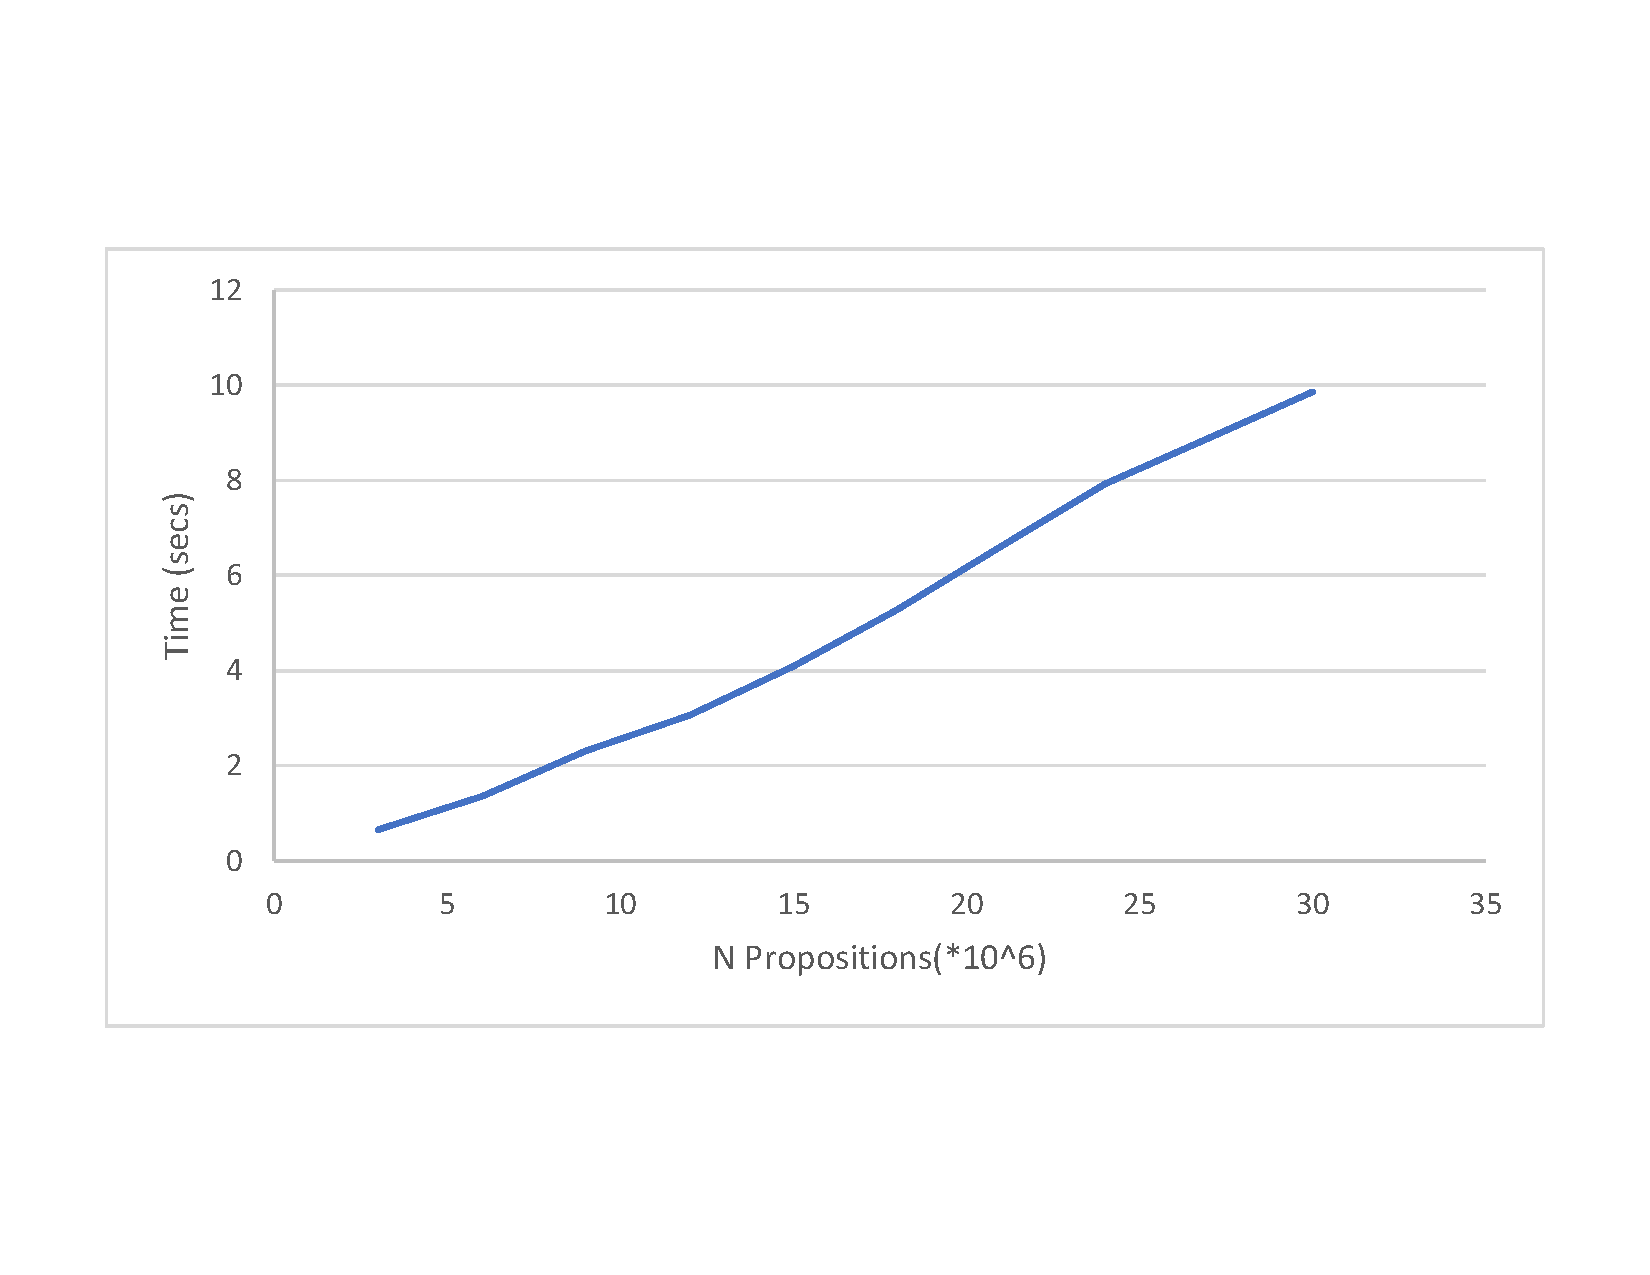
\includegraphics[width=12cm,height=8cm, trim=1.5cm 3.6cm 0cm 4.2cm, clip=true, natwidth=6in, natheight=44in]{time_graphProp2.pdf}
\caption{Times for Bottom-up Evaluation of Triangular Programs}\label{buperftable}
\end{figure}

Times are just for the meta-interpretation of the triangular programs;
the time for generating the {\tt (<-)/2} facts for the programs is not
included. The graph is essentially a straight line, showing the
linearity of the algorithm.  The propositional Horn clause
satisfaction problem is known to be linear in the number of
proposition occurrences \cite{Dowling1984LinearTimeAF}, and this
meta-interpreter is indeed linear on all propositional logic programs.

Triangular programs have no loops so pure top-down evaluation without
tabling will terminate, but will be very slow due to many redundant
computations.  For example to evaluate without tabling the single
query, {\tt p1}, to a triangular program with 325 proposition
occurrences takes c. 4.1 seconds, and with 465 occurrences c. 126
seconds.  This contrasts with the 15,000,000 occurrences in the
program that is computed by tabled bottom-up evaluation in 4.1 seconds
(as shown in the figure).


\section{Conclusion}
In this paper we have described the integration of bottom-up
evaluation with top-down evaluation in tabled Prolog by means of
Subsumptive Tabling With Abstraction (STWA).  We provided a procedural
interpretation for bottom-up evaluation, in the context of Prolog
programming, as efficient indexed data structure initialization.  This
allows many formerly non-declarative Prolog programs that contain
assert/1 to be naturally expressed as declarative programs with no
sacrifice in efficiency.

We have shown how XSB provides a natural model for evaluating Horn
programs, based on nondeterministic procedural interpretation using
subsumptive tabling with abstraction, that incorporates both top-down
and bottom-up computation in a single uniform framework.  And this
model provides linear evaluation of all queries to proposition Horn
programs for all intermixings of demand and data driven computation.

\section{Programs to Generate Traces} \label{progs}
Program that generates trace of bottom-up evaluation of {\tt ?- p(a,X).}
\footnotesize
\begin{verbatim}
:- table_index(p/2,[1,0]).
p(X,Y) :-
    writeln('enter rule 1: p'(X,Y)),
    e(X,Y),
    write('from fact: e'(X,Y)),
    write(' infer p'(X,Y)),
p(X,Y) :-
    writeln('enter rule 2 p'(X,Y)),
    p(X,Z),
    write('from table: p'(X,Z)),
    e(Z,Y),
    write(' and fact e'(Z,Y)),
    write(' infer p'(X,Y)).            

e(a,b).     e(b,c).
e(e,a).     e(c,b).
e(d,e).
\end{verbatim}
\normalsize

Program that generates the annotated trace of bottom-up
meta-interpretation of proposition clauses.
\footnotesize
\begin{verbatim}
:- op(1200,xfx,('<-')).
:- import conset/2, coninc/2 from gensym.

:- table_index(interpAtom/1,[0]).
interpAtom(G) :-
    conset('_ctr',0),
    log('%S demanded',args(G)),
    (G <- Body),
    log('%S :- %S initial clause',args(G,Body)),
    interp(Body,G).

interp(true,H) :- !, log('%S from true and %S :- true',args(H,H)).
interp((A,B),H) :- !,
    interpAtom(A),
    log('%S :- %S from %S and %S :- %S',args(H,B,A,H,(A,B))),
    interp(B,H).
interp(G,H) :-
    interpAtom(G),
    log('%S from %S and %S :- %S',args(H,G,H,G)).

p <- q,v,r,s.          s <- true.
p <- q,s,t.            u <- s,p,v,r.
q <- u,r.              u <- r,t.
q <- q,t,v.            t <- true.
r <- s.
\end{verbatim}
\normalsize

\section{Subsumptive Tabling with Full Abstraction (STWFA) is Bottom-up}
\label{app-proof}
This section proves a close relationship between the evaluation of
Horn programs using subsumptive tabling with full abstraction and
their bottom-up evaluation.

\subsection{Multiple Machine Model of Tabled Horn Clause Evaluation}
We describe a model for STWFA evaluation as a set of (virtual)
machines.  Given a Horn clause program and a goal, each machine
carries out the evaluation of the goal in the program along a
different deterministic path.  Without tabling there would be a
machine corresponding to each root-to-leaf path of the SLD tree for
the query.  With subsumptive tabling with full abstraction, the model
is as described next.

A global table of subgoals is maintained.  Associated with each
subgoal is a set of answers corresponding to proven instances of the
subgoal.  This table is maintained and used by all the executing
machines.  It is monotonic in that goals and answers are only added to
the table and never deleted.

Computation starts with a single machine that is given the initial
goal to evaluate.  When a machine encounters a goal, it looks to see
if the corresponding most-general goal is in the global table.  If it
is {\em not} in the table, a) it adds it (with an empty list of
associated answers), b) for each clause for that most-general goal, it
forks off a duplicate of itself to process it, and c) remembering the
goal it encountered, it suspends on the table entry it just added (to
later process answers that are associated with that most-general
goal).  If the most-general goal already {\em is} in the table, the
machine (remembering its encountered goal) suspends on that table
entry.

When a machine encounters a failure, it simply disappears.  When a
machine returns an answer to a goal (i.e., completes execution to the
end of a clause for that goal), it adds the computed goal instance to
the end of the list of answers associated with that goal in the table,
and then disappears.

Whenever there is a new answer for a table entry for a goal, each machine
that is suspended on that entry, whose associated goal unifies with
that new answer, forks off a copy of itself.  This new machine uses
that answer to update its state and then continues executing.  The
suspended machine remains suspended having marked in the table that
that answer has been returned.

This set of machines is normally simulated by a sequential emulator,
which includes a scheduler that determines which of the next possible
machine operations will be performed.  At any point in the execution,
there may be a machine ready to a) evaluate the next goal of some
clause (or return an answer if there are no more goals for that
clause) or b) fork a machine that is suspended on a table entry to
process a new (unifying) answer.  For specificity and simplicity, we
will assume that answers associated with a table entry are maintained
in the order they are generated, and suspended machines return them in
that same order.

\subsection{Example of STWFA Evaluation}

To better understand this model, we trace its evaluation of the graph
reachability example, with the edge relation defined by a simple join:
\footnotesize
\begin{verbatim}
:- table_index(p/2,[0]).
                             q(a,b).           r(a).
p(X,Y) :- e(X,Y).            q(a,d).           r(b).
p(X,Y) :- p(X,Z),e(Z,Y).     q(e,a).           r(c).
                             q(d,e). q(b,d).   r(e).
e(X,Y) :- q(X,Y),r(Y).       q(b,c). q(c,b).
\end{verbatim}
\normalsize

We trace the evaluation of the query p(a,X).  A state of a machine is
represented by a rule form: $H\leftarrow B_1,B_2,...,B_k$, where $k>=0$.
This represents a machine about to call subgoal $B_1$, which on its
return will be followed by calls to $B_2$ through $B_k$, and then a
return to $H$.  When $k=0$, it is about to return the answer H to its
call.

The table is represented by a set of forms: $Goal:[AnsList],[H\leftarrow
  B_1,B_2,...,B_k:N,...]$ where $Goal$ is a most-general goal,
$AnsList$ is a list of instances of Goal (a.k.a. answers). The indexed
rule form $H\leftarrow B_1,B_2,...,B_k:N$ represents a suspension:
$B_1$ is an instance of $Goal$, and $N$ is an integer between $0$ and
the length of the answer list, and is the index of the last answer
from $B_1$ that has been returned, i.e., for which the suspension has
been cloned and continued.  This pair of a rule and index represents a
machine that is suspended on the goal of this table entry; there may
be multiple such suspensions.

In the following trace, \verb|S:| indicates the set of machine states
that are available to be scheduled, separated by semi-colons and
\verb|T:| indicates the state of the table.  We trace the evaluation
of the query \verb|p(a,X)|.

\footnotesize
\begin{verbatim}
S: <-p(a,X)
T:

Create new table entry for p/2, suspend on it, fork machines for each rule:
S: p(X,Y)<-e(X,Y); p(X,Y)<-p(X,Z),e(Z,Y)
T: p(X,Y):[],[<-p(a,X):0]

Create new table entry for e/2, suspend on it, fork machines for each rule:
S: e(X,Y)<-q(X,Y),r(Y); p(X,Y)<-p(X,Z),e(Z,Y)
T: p(X,Y):[],[<-p(a,X):0]
   e(X,Y):[],[p(X,Y)<-e(X,Y):0]

Create new table entry for q/2, suspend, fork machines for each rule:
S: q(a,b)<-; q(a,d)<-; q(e,a)<-; q(d,e)<-; q(b,c)<-; q(b,d)<-; q(c,b)<-;
   p(X,Y)<-p(X,Z),e(Z,Y)
T: p(X,Y):[],[<-p(a,X):0]
   e(X,Y):[],[p(X,Y)<-e(X,Y):0]
   q(X,Y):[],[e(X,Y)<-q(X,Y),r(Y):0]

7 steps, returning q/2 facts to the q(X,Y), adding them to its table:
S: p(X,Y)<-p(X,Z),e(Z,Y)
T: p(X,Y):[],[<-p(a,X):0]
   e(X,Y):[],[p(X,Y)<-e(X,Y):0]
   q(X,Y):[q(a,b),q(a,d),q(e,a),q(d,e),q(b,c),q(b,d),q(c,b)],
          [e(X,Y)<-q(X,Y),r(Y):0]

Fork off 7 copies of the suspended e<-q,r machine, one for each answer:
S: e(a,b)<-r(b); e(a,d)<-r(d); e(e,a)<-r(a); e(d,e)<-r(e); e(b,c)<-r(c);
   e(b,d)<-r(d); e(c,b)<-r(b); p(X,Y)<-p(X,Z),e(Z,Y)
T: p(X,Y):[],[<-p(a,X):0]
   e(X,Y):[],[p(X,Y)<-e(X,Y):0]
   q(X,Y):[q(a,b),q(a,d),q(e,a),q(d,e),q(b,c),q(b,d),q(c,b)],
          [e(X,Y)<-q(X,Y),r(Y):7]

Create new table entry for r/1, suspend on it, fork one for each r/1 rule:
S: r(a)<-; r(b)<-; r(c)<-; r(e)<-;
   e(a,d)<-r(d); e(e,a)<-r(a); e(d,e)<-r(e); e(b,c)<-r(c); e(b,d)<-r(d)
   e(c,b)<-r(b); p(X,Y)<-p(X,Z),e(Z,Y)
T: p(X,Y):[],[<-p(a,X):0]
   e(X,Y):[],[p(X,Y)<-e(X,Y):0]a
   q(X,Y):[q(a,b),q(a,d),q(e,a),q(d,e),q(b,c),q(b,d),q(c,b)],
          [e(X,Y)<-q(X,Y),r(Y):7]
   r(X):[],[e(a,b)<-r(b):0]

4 steps, returning 4 answers to r/1 call:
S: e(a,d)<-r(d); e(e,a)<-r(a); e(d,e)<-r(e); e(b,c)<-r(c); e(b,d)<-r(d);
   e(c,b)<-r(b); p(X,Y)<-p(X,Z),e(Z,Y)
T: p(X,Y):[],[<-p(a,X):0]
   e(X,Y):[],[p(X,Y)<-e(X,Y):0]
   q(X,Y):[q(a,b),q(a,d),q(e,a),q(d,e),q(b,c),q(b,d),q(c,b)],
          [e(X,Y)<-q(X,Y),r(Y):7]
   r(X):[r(a),r(b),r(c),r(e)],[e(a,b)<-r(b):0]

7 steps each calling r/1 and suspending on that call:
S: p(X,Y)<-p(X,Z),e(Z,Y)
T: p(X,Y):[],[<-p(a,X):0]
   e(X,Y):[],[p(X,Y)<-e(X,Y):0]
   q(X,Y):[q(a,b),q(a,d),q(e,a),q(d,e),q(b,c),q(b,d),q(c,b)],
          [e(X,Y)<-q(X,Y),r(Y):7]
   r(X):[r(a),r(b),r(c),r(e)],
        [e(a,b)<-r(b):0, e(a,d)<-r(d):0, e(e,a)<-r(a):0,
         e(d,e)<-r(e):0, e(b,c)<-r(c):0, e(b,d)<-r(d):0,
         e(c,b)<-r(b):0]

7 (*4) steps returning r/1 answers to suspended machine.  5 of the
  suspended machines match on answer and 2 match no answers, generating
  5 new machines:
S: e(a,b)<-; e(e,a)<-; e(d,e)<-; e(b,c)<-; e(c,b)<-; 
p(X,Y)<-p(X,Z),e(Z,Y)
T: p(X,Y):[],[<-p(a,X):0]
   e(X,Y):[],[p(X,Y)<-e(X,Y):0]
   q(X,Y):[q(a,b),q(a,d),q(e,a),q(d,e),q(b,c),q(b,d),q(c,b)],
          [e(X,Y)<-q(X,Y),r(Y):7]
   r(X):[r(a),r(b),r(c),r(e)],
        [e(a,b)<-r(b):4, e(a,d)<-r(d):4, e(e,a)<-r(a):4,
         e(d,e)<-r(e):4, e(b,c)<-r(c):4, e(b,d)<-r(d):4,
         e(c,b)<-r(b):4]

5 steps returning 5 answers to the e/2 table:
S: p(X,Y)<-p(X,Z),e(Z,Y)
T: p(X,Y):[],[<-p(a,X):0]
   e(X,Y):[e(a,b),e(e,a),e(d,e),e(b,c),e(c,b)],[p(X,Y)<-e(X,Y):0]
   q(X,Y):[q(a,b),q(a,d),q(e,a),q(d,e),q(b,c),q(b,d),q(c,b)],
          [e(X,Y)<-q(X,Y),r(Y):7]
   r(X):[r(a),r(b),r(c),r(e)],
        [e(a,b)<-r(b):4, e(a,d)<-r(d):4, e(e,a)<-r(a):4,
         e(d,e)<-r(e):4, e(b,c)<-r(c):4, e(b,d)<-r(d):4,
         e(c,b)<-r(b):4]

The machine suspended on e/2 forks 5 new machines, one for each new answer:
S: p(a,b)<-; p(e,a)<- ; p(d,e)<-; p(b,c)<-; p(c,b)<-; p(X,Y)<-p(X,Z),e(Z,Y)
T: p(X,Y):[],[<-p(a,X):0]
   e(X,Y):[e(a,b),e(e,a),e(d,e),e(b,c),e(c,b)],[p(X,Y)<-e(X,Y):5]
   q(X,Y):[q(a,b),q(a,d),q(e,a),q(d,e),q(b,c),q(b,d),q(c,b)],
          [e(X,Y)<-q(X,Y),r(Y):7]
   r(X):[r(a),r(b),r(c),r(e)],
        [e(a,b)<-r(b):4, e(a,d)<-r(d):4, e(e,a)<-r(a):4,
         e(d,e)<-r(e):4, e(b,c)<-r(c):4, e(b,d)<-r(d):4,
         e(c,b)<-r(b):4]

5 steps, adding 5 new answers to p/2 entry:
S: p(X,Y)<-p(X,Z),e(Z,Y)
T: p(X,Y):[p(a,b),p(e,a),p(d,e),p(b,c),p(c,b)],[<-p(a,X):0]
   e(X,Y):[e(a,b),e(e,a),e(d,e),e(b,c),e(c,b)],[p(X,Y)<-e(X,Y):5]
   q(X,Y):[q(a,b),q(a,d),q(e,a),q(d,e),q(b,c),q(b,d),q(c,b)],
          [e(X,Y)<-q(X,Y),r(Y):7]
   r(X):[r(a),r(b),r(c),r(e)],
        [e(a,b)<-r(b):4, e(a,d)<-r(d):4, e(e,a)<-r(a):4,
         e(d,e)<-r(e):4, e(b,c)<-r(c):4, e(b,d)<-r(d):4,
         e(c,b)<-r(b):4]

Machine suspends on call to p(X,Z):
S: 
T: p(X,Y):[p(a,b),p(e,a),p(d,e),p(b,c),p(c,b)],[<-p(a,X):0,p(X,Y)<-p(X,Z),e(Z,Y):0]
   e(X,Y):[e(a,b),e(e,a),e(d,e),e(b,c),e(c,b)],[p(X,Y)<-e(X,Y):5]
   q(X,Y):[q(a,b),q(a,d),q(e,a),q(d,e),q(b,c),q(b,d),q(c,b)],
          [e(X,Y)<-q(X,Y),r(Y):7]
   r(X):[r(a),r(b),r(c),r(e)],
        [e(a,b)<-r(b):4, e(a,d)<-r(d):4, e(e,a)<-r(a):4,
         e(d,e)<-r(e):4, e(b,c)<-r(c):4, e(b,d)<-r(d):4,
         e(c,b)<-r(b):4]

5 new machines forked from machine suspended on p/2:
S: p(a,Y)<-e(b,Y); p(e,Y)<-e(a,Y); p(d,Y)<-e(e,Y); p(b,Y)<-e(c,Y); p(c,Y)<-e(b,Y)        
T: p(X,Y):[p(a,b),p(e,a),p(d,e),p(b,c),p(c,b)],[<-p(a,X):0,p(X,Y)<-p(X,Z),e(Z,Y):5]
   e(X,Y):[e(a,b),e(e,a),e(d,e),e(b,c),e(c,b)],[p(X,Y)<-e(X,Y):5]
   q(X,Y):[q(a,b),q(a,d),q(e,a),q(d,e),q(b,c),q(b,d),q(c,b)],
          [e(X,Y)<-q(X,Y),r(Y):7]
   r(X):[r(a),r(b),r(c),r(e)],
        [e(a,b)<-r(b):4, e(a,d)<-r(d):4, e(e,a)<-r(a):4,
         e(d,e)<-r(e):4, e(b,c)<-r(c):4, e(b,d)<-r(d):4,
         e(c,b)<-r(b):4]

All 5 just generated machines suspend on their calls to e/2:
S: 
T: p(X,Y):[p(a,b),p(e,a),p(d,e),p(b,c),p(c,b)],[<-p(a,X):0,p(X,Y)<-p(X,Z),e(Z,Y):5]
   e(X,Y):[e(a,b),e(e,a),e(d,e),e(b,c),e(c,b)],
          [p(X,Y)<-e(X,Y):5, p(a,Y)<-e(b,Y):0, p(e,Y)<-e(a,Y):0,
           p(d,Y)<-e(e,Y):0, p(b,Y)<-e(c,Y):0, p(c,Y)<-e(b,Y):0]
   q(X,Y):[q(a,b),q(a,d),q(e,a),q(d,e),q(b,c),q(b,d),q(c,b)],
          [e(X,Y)<-q(X,Y),r(Y):7]
   r(X):[r(a),r(b),r(c),r(e)],
        [e(a,b)<-r(b):4, e(a,d)<-r(d):4, e(e,a)<-r(a):4,
         e(d,e)<-r(e):4, e(b,c)<-r(c):4, e(b,d)<-r(d):4,
         e(c,b)<-r(b):4]

The 5 just suspended machines fork of 5 new machines; each machine
  matching exactly one of the 5 new answers:
S: p(a,c)<-; p(e,b)<-; p(d,a)<-; p(b,b)<-; p(c,c)<-
T: p(X,Y):[p(a,b),p(e,a),p(d,e),p(b,c),p(c,b)],[<-p(a,X):0,p(X,Y)<-p(X,Z),e(Z,Y):5]
   e(X,Y):[e(a,b),e(e,a),e(d,e),e(b,c),e(c,b)],
          [p(X,Y)<-e(X,Y):5, p(a,Y)<-e(b,Y):5, p(e,Y)<-e(a,Y):5,
           p(d,Y)<-e(e,Y):5, p(b,Y)<-e(c,Y):5, p(c,Y)<-e(b,Y):5]
   q(X,Y):[q(a,b),q(a,d),q(e,a),q(d,e),q(b,c),q(b,d),q(c,b)],
          [e(X,Y)<-q(X,Y),r(Y):7]
   r(X):[r(a),r(b),r(c),r(e)],
        [e(a,b)<-r(b):4, e(a,d)<-r(d):4, e(e,a)<-r(a):4,
         e(d,e)<-r(e):4, e(b,c)<-r(c):4, e(b,d)<-r(d):4,
         e(c,b)<-r(b):4]

Each of the 5 new machines add a new answer to the p/2 table entry:
S:
T: p(X,Y):[p(a,b),p(e,a),p(d,e),p(b,c),p(c,b),p(a,c),p(e,b),p(d,a),p(b,b),p(c,c)],
             [<-p(a,X):0,p(X,Y)<-p(X,Z),e(Z,Y):5]
   e(X,Y):[e(a,b),e(e,a),e(d,e),e(b,c),e(c,b)],
          [p(X,Y)<-e(X,Y):5, p(a,Y)<-e(b,Y):5, p(e,Y)<-e(a,Y):5,
           p(d,Y)<-e(e,Y):5, p(b,Y)<-e(c,Y):5, p(c,Y)<-e(b,Y):5]
   q(X,Y):[q(a,b),q(a,d),q(e,a),q(d,e),q(b,c),q(b,d),q(c,b)],
          [e(X,Y)<-q(X,Y),r(Y):7]
   r(X):[r(a),r(b),r(c),r(e)],
        [e(a,b)<-r(b):4, e(a,d)<-r(d):4, e(e,a)<-r(a):4,
         e(d,e)<-r(e):4, e(b,c)<-r(c):4, e(b,d)<-r(d):4,
         e(c,b)<-r(b):4]

The machine suspended on p(X,Z) in the p/2 table forks off machines
  for each of the 5 just-add p/2 answers:
S: p(a,Y)<-e(c,Y); p(e,Y)<-e(b,Y); p(d,Y)<-e(a,Y); p(b,Y)<-e(b,Y); p(c,Y)<-e(c,Y)
T: p(X,Y):[p(a,b),p(e,a),p(d,e),p(b,c),p(c,b),p(a,c),p(e,b),p(d,a),p(b,b),p(c,c)],
             [<-p(a,X):0,p(X,Y)<-p(X,Z),e(Z,Y):10]
   e(X,Y):[e(a,b),e(e,a),e(d,e),e(b,c),e(c,b)],
          [p(X,Y)<-e(X,Y):5, p(a,Y)<-e(b,Y):5, p(e,Y)<-e(a,Y):5,
           p(d,Y)<-e(e,Y):5, p(b,Y)<-e(c,Y):5, p(c,Y)<-e(b,Y):5]
   q(X,Y):[q(a,b),q(a,d),q(e,a),q(d,e),q(b,c),q(b,d),q(c,b)],
          [e(X,Y)<-q(X,Y),r(Y):7]
   r(X):[r(a),r(b),r(c),r(e)],
        [e(a,b)<-r(b):4, e(a,d)<-r(d):4, e(e,a)<-r(a):4,
         e(d,e)<-r(e):4, e(b,c)<-r(c):4, e(b,d)<-r(d):4,
         e(c,b)<-r(b):4]

All 5 of those machines suspend on their calls to e/2.
S: 
T: p(X,Y):[p(a,b),p(e,a),p(d,e),p(b,c),p(c,b),p(a,c),p(e,b),p(d,a),p(b,b),p(c,c)],
             [<-p(a,X):0,p(X,Y)<-p(X,Z),e(Z,Y):10]
   e(X,Y):[e(a,b),e(e,a),e(d,e),e(b,c),e(c,b)],
          [p(X,Y)<-e(X,Y):5, p(a,Y)<-e(b,Y):5, p(e,Y)<-e(a,Y):5,
           p(d,Y)<-e(e,Y):5, p(b,Y)<-e(c,Y):5, p(c,Y)<-e(b,Y):5,
           p(a,Y)<-e(c,Y):0, p(e,Y)<-e(b,Y):0, p(d,Y)<-e(a,Y):0,
           p(b,Y)<-e(b,Y):0,  p(c,Y)<-e(c,Y):0]
   q(X,Y):[q(a,b),q(a,d),q(e,a),q(d,e),q(b,c),q(b,d),q(c,b)],
          [e(X,Y)<-q(X,Y),r(Y):7]
   r(X):[r(a),r(b),r(c),r(e)],
        [e(a,b)<-r(b):4, e(a,d)<-r(d):4, e(e,a)<-r(a):4,
         e(d,e)<-r(e):4, e(b,c)<-r(c):4, e(b,d)<-r(d):4,
         e(c,b)<-r(b):4]

All 5 of those suspensions fork off a total of 5 new machines, each
  one matching one of the 5 existing answers for e/2:
S: p(a,b)<-; p(e,c)<-; p(d,b)<-; p(b,c)<-; p(c,b)<-       
T: p(X,Y):[p(a,b),p(e,a),p(d,e),p(b,c),p(c,b),p(a,c),p(e,b),p(d,a),p(b,b),p(c,c)],
             [<-p(a,X):0,p(X,Y)<-p(X,Z),e(Z,Y):10]
   e(X,Y):[e(a,b),e(e,a),e(d,e),e(b,c),e(c,b)],
          [p(X,Y)<-e(X,Y):5, p(a,Y)<-e(b,Y):5, p(e,Y)<-e(a,Y):5,
           p(d,Y)<-e(e,Y):5, p(b,Y)<-e(c,Y):5, p(c,Y)<-e(b,Y):5,
           p(a,Y)<-e(c,Y):5, p(e,Y)<-e(b,Y):5, p(d,Y)<-e(a,Y):5,
           p(b,Y)<-e(b,Y):5, p(c,Y)<-e(c,Y):5]
   q(X,Y):[q(a,b),q(a,d),q(e,a),q(d,e),q(b,c),q(b,d),q(c,b)],
          [e(X,Y)<-q(X,Y),r(Y):7]
   r(X):[r(a),r(b),r(c),r(e)],
        [e(a,b)<-r(b):4, e(a,d)<-r(d):4, e(e,a)<-r(a):4,
         e(d,e)<-r(e):4, e(b,c)<-r(c):4, e(b,d)<-r(d):4,
         e(c,b)<-r(b):4]

Those 5 machines return just 2 new answers to the p/2 entry (3 are duplicates):
S:
T: p(X,Y):[p(a,b),p(e,a),p(d,e),p(b,c),p(c,b),p(a,c),p(e,b),p(d,a),p(b,b),p(c,c),
              p(e,c),p(d,b)],
             [<-p(a,X):0,p(X,Y)<-p(X,Z),e(Z,Y):10]
   e(X,Y):[e(a,b),e(e,a),e(d,e),e(b,c),e(c,b)],
          [p(X,Y)<-e(X,Y):5, p(a,Y)<-e(b,Y):5, p(e,Y)<-e(a,Y):5,
           p(d,Y)<-e(e,Y):5, p(b,Y)<-e(c,Y):5, p(c,Y)<-e(b,Y):5,
           p(a,Y)<-e(c,Y):5, p(e,Y)<-e(b,Y):5, p(d,Y)<-e(a,Y):5,
           p(b,Y)<-e(b,Y):5, p(c,Y)<-e(c,Y):5]
   q(X,Y):[q(a,b),q(a,d),q(e,a),q(d,e),q(b,c),q(b,d),q(c,b)],
          [e(X,Y)<-q(X,Y),r(Y):7]
   r(X):[r(a),r(b),r(c),r(e)],
        [e(a,b)<-r(b):4, e(a,d)<-r(d):4, e(e,a)<-r(a):4,
         e(d,e)<-r(e):4, e(b,c)<-r(c):4, e(b,d)<-r(d):4,
         e(c,b)<-r(b):4]

The suspend p<-p,e machine forks 2 new machines, one for each just-added answer;
S: p(e,Y)<-e(c,Y); p(d,Y)<-e(b,Y)
T: p(X,Y):[p(a,b),p(e,a),p(d,e),p(b,c),p(c,b),p(a,c),p(e,b),p(d,a),p(b,b),p(c,c),
              p(e,c),p(d,b)],
             [<-p(a,X):0,p(X,Y)<-p(X,Z),e(Z,Y):12]
   e(X,Y):[e(a,b),e(e,a),e(d,e),e(b,c),e(c,b)],
          [p(X,Y)<-e(X,Y):5, p(a,Y)<-e(b,Y):5, p(e,Y)<-e(a,Y):5,
           p(d,Y)<-e(e,Y):5, p(b,Y)<-e(c,Y):5, p(c,Y)<-e(b,Y):5,
           p(a,Y)<-e(c,Y):5, p(e,Y)<-e(b,Y):5, p(d,Y)<-e(a,Y):5,
           p(b,Y)<-e(b,Y):5, p(c,Y)<-e(c,Y):5]
   q(X,Y):[q(a,b),q(a,d),q(e,a),q(d,e),q(b,c),q(b,d),q(c,b)],
          [e(X,Y)<-q(X,Y),r(Y):7]
   r(X):[r(a),r(b),r(c),r(e)],
        [e(a,b)<-r(b):4, e(a,d)<-r(d):4, e(e,a)<-r(a):4,
         e(d,e)<-r(e):4, e(b,c)<-r(c):4, e(b,d)<-r(d):4,
         e(c,b)<-r(b):4]

Those 2 new machines suspend on their e/2 calls:
S: 
T: p(X,Y):[p(a,b),p(e,a),p(d,e),p(b,c),p(c,b),p(a,c),p(e,b),p(d,a),p(b,b),p(c,c),
              p(e,c),p(d,b)],
             [<-p(a,X):0,p(X,Y)<-p(X,Z),e(Z,Y):12]
   e(X,Y):[e(a,b),e(e,a),e(d,e),e(b,c),e(c,b)],
          [p(X,Y)<-e(X,Y):5, p(a,Y)<-e(b,Y):5, p(e,Y)<-e(a,Y):5,
           p(d,Y)<-e(e,Y):5, p(b,Y)<-e(c,Y):5, p(c,Y)<-e(b,Y):5,
           p(a,Y)<-e(c,Y):5, p(e,Y)<-e(b,Y):5, p(d,Y)<-e(a,Y):5,
           p(b,Y)<-e(b,Y):5, p(c,Y)<-e(c,Y):5, p(e,Y)<-e(c,Y):0
           p(d,Y)<-e(b,Y):0]
   q(X,Y):[q(a,b),q(a,d),q(e,a),q(d,e),q(b,c),q(b,d),q(c,b)],
          [e(X,Y)<-q(X,Y),r(Y):7]
   r(X):[r(a),r(b),r(c),r(e)],
        [e(a,b)<-r(b):4, e(a,d)<-r(d):4, e(e,a)<-r(a):4,
         e(d,e)<-r(e):4, e(b,c)<-r(c):4, e(b,d)<-r(d):4,
         e(c,b)<-r(b):4]

Those 2 suspensions fork 2 new machines from all the e/2 answers,
  each matching exactly one:
S: p(e,b)<-; p(d,c)<-
T: p(X,Y):[p(a,b),p(e,a),p(d,e),p(b,c),p(c,b),p(a,c),p(e,b),p(d,a),p(b,b),p(c,c),
              p(e,c),p(d,b)],
             [<-p(a,X):0,p(X,Y)<-p(X,Z),e(Z,Y):12]
   e(X,Y):[e(a,b),e(e,a),e(d,e),e(b,c),e(c,b)],
          [p(X,Y)<-e(X,Y):5, p(a,Y)<-e(b,Y):5, p(e,Y)<-e(a,Y):5,
           p(d,Y)<-e(e,Y):5, p(b,Y)<-e(c,Y):5, p(c,Y)<-e(b,Y):5,
           p(a,Y)<-e(c,Y):5, p(e,Y)<-e(b,Y):5, p(d,Y)<-e(a,Y):5,
           p(b,Y)<-e(b,Y):5, p(c,Y)<-e(c,Y):5, p(e,Y)<-e(c,Y):5,
           p(d,Y)<-e(b,Y):5]
   q(X,Y):[q(a,b),q(a,d),q(e,a),q(d,e),q(b,c),q(b,d),q(c,b)],
          [e(X,Y)<-q(X,Y),r(Y):7]
   r(X):[r(a),r(b),r(c),r(e)],
        [e(a,b)<-r(b):4, e(a,d)<-r(d):4, e(e,a)<-r(a):4,
         e(d,e)<-r(e):4, e(b,c)<-r(c):4, e(b,d)<-r(d):4,
         e(c,b)<-r(b):4]

These two machines add just one new answer to the p/2 table entry:
S:
T: p(X,Y):[p(a,b),p(e,a),p(d,e),p(b,c),p(c,b),p(a,c),p(e,b),p(d,a),p(b,b),p(c,c),
              p(e,c),p(d,b),p(d,c)],
             [<-p(a,X):0,p(X,Y)<-p(X,Z),e(Z,Y):12]
   e(X,Y):[e(a,b),e(e,a),e(d,e),e(b,c),e(c,b)],
          [p(X,Y)<-e(X,Y):5, p(a,Y)<-e(b,Y):5, p(e,Y)<-e(a,Y):5,
           p(d,Y)<-e(e,Y):5, p(b,Y)<-e(c,Y):5, p(c,Y)<-e(b,Y):5,
           p(a,Y)<-e(c,Y):5, p(e,Y)<-e(b,Y):5, p(d,Y)<-e(a,Y):5,
           p(b,Y)<-e(b,Y):5, p(c,Y)<-e(c,Y):5, p(e,Y)<-e(c,Y):5,
           p(d,Y)<-e(b,Y):5]
   q(X,Y):[q(a,b),q(a,d),q(e,a),q(d,e),q(b,c),q(b,d),q(c,b)],
          [e(X,Y)<-q(X,Y),r(Y):7]
   r(X):[r(a),r(b),r(c),r(e)],
        [e(a,b)<-r(b):4, e(a,d)<-r(d):4, e(e,a)<-r(a):4,
         e(d,e)<-r(e):4, e(b,c)<-r(c):4, e(b,d)<-r(d):4,
         e(c,b)<-r(b):4]

The p<-p,e suspension on p/2 forks off a new machine for that new answer:
S: p(d,Y)<-e(c,Y)
T: p(X,Y):[p(a,b),p(e,a),p(d,e),p(b,c),p(c,b),p(a,c),p(e,b),p(d,a),p(b,b),p(c,c),
              p(e,c),p(d,b),p(d,c)],
             [<-p(a,X):0,p(X,Y)<-p(X,Z),e(Z,Y):13]
   e(X,Y):[e(a,b),e(e,a),e(d,e),e(b,c),e(c,b)],
          [p(X,Y)<-e(X,Y):5, p(a,Y)<-e(b,Y):5, p(e,Y)<-e(a,Y):5,
           p(d,Y)<-e(e,Y):5, p(b,Y)<-e(c,Y):5, p(c,Y)<-e(b,Y):5,
           p(a,Y)<-e(c,Y):5, p(e,Y)<-e(b,Y):5, p(d,Y)<-e(a,Y):5,
           p(b,Y)<-e(b,Y):5, p(c,Y)<-e(c,Y):5, p(e,Y)<-e(c,Y):5,
           p(d,Y)<-e(b,Y):5]
   q(X,Y):[q(a,b),q(a,d),q(e,a),q(d,e),q(b,c),q(b,d),q(c,b)],
          [e(X,Y)<-q(X,Y),r(Y):7]
   r(X):[r(a),r(b),r(c),r(e)],
        [e(a,b)<-r(b):4, e(a,d)<-r(d):4, e(e,a)<-r(a):4,
         e(d,e)<-r(e):4, e(b,c)<-r(c):4, e(b,d)<-r(d):4,
         e(c,b)<-r(b):4]

That machine calls e/2 and suspends:
S: 
T: p(X,Y):[p(a,b),p(e,a),p(d,e),p(b,c),p(c,b),p(a,c),p(e,b),p(d,a),p(b,b),p(c,c),
              p(e,c),p(d,b),p(d,c)],
             [<-p(a,X):0,p(X,Y)<-p(X,Z),e(Z,Y):13]
   e(X,Y):[e(a,b),e(e,a),e(d,e),e(b,c),e(c,b)],
          [p(X,Y)<-e(X,Y):5, p(a,Y)<-e(b,Y):5, p(e,Y)<-e(a,Y):5,
           p(d,Y)<-e(e,Y):5, p(b,Y)<-e(c,Y):5, p(c,Y)<-e(b,Y):5,
           p(a,Y)<-e(c,Y):5, p(e,Y)<-e(b,Y):5, p(d,Y)<-e(a,Y):5,
           p(b,Y)<-e(b,Y):5, p(c,Y)<-e(c,Y):5, p(e,Y)<-e(c,Y):5,
           p(d,Y)<-e(b,Y):5, p(d,Y)<-e(c,Y):0]
   q(X,Y):[q(a,b),q(a,d),q(e,a),q(d,e),q(b,c),q(b,d),q(c,b)],
          [e(X,Y)<-q(X,Y),r(Y):7]
   r(X):[r(a),r(b),r(c),r(e)],
        [e(a,b)<-r(b):4, e(a,d)<-r(d):4, e(e,a)<-r(a):4,
         e(d,e)<-r(e):4, e(b,c)<-r(c):4, e(b,d)<-r(d):4,
         e(c,b)<-r(b):4]

That suspension forks one machine for the one matching answer in e/2:
S: p(d,b)<-
T: p(X,Y):[p(a,b),p(e,a),p(d,e),p(b,c),p(c,b),p(a,c),p(e,b),p(d,a),p(b,b),p(c,c),
              p(e,c),p(d,b),p(d,c)],
             [<-p(a,X):0,p(X,Y)<-p(X,Z),e(Z,Y):13]
   e(X,Y):[e(a,b),e(e,a),e(d,e),e(b,c),e(c,b)],
          [p(X,Y)<-e(X,Y):5, p(a,Y)<-e(b,Y):5, p(e,Y)<-e(a,Y):5,
           p(d,Y)<-e(e,Y):5, p(b,Y)<-e(c,Y):5, p(c,Y)<-e(b,Y):5,
           p(a,Y)<-e(c,Y):5, p(e,Y)<-e(b,Y):5, p(d,Y)<-e(a,Y):5,
           p(b,Y)<-e(b,Y):5, p(c,Y)<-e(c,Y):5, p(e,Y)<-e(c,Y):5,
           p(d,Y)<-e(b,Y):5, p(d,Y)<-e(c,Y):5]
   q(X,Y):[q(a,b),q(a,d),q(e,a),q(d,e),q(b,c),q(b,d),q(c,b)],
          [e(X,Y)<-q(X,Y),r(Y):7]
   r(X):[r(a),r(b),r(c),r(e)],
        [e(a,b)<-r(b):4, e(a,d)<-r(d):4, e(e,a)<-r(a):4,
         e(d,e)<-r(e):4, e(b,c)<-r(c):4, e(b,d)<-r(d):4,
         e(c,b)<-r(b):4]

That machine fails since the answer it wants to add is a duplicate:
S: 
T: p(X,Y):[p(a,b),p(e,a),p(d,e),p(b,c),p(c,b),p(a,c),p(e,b),p(d,a),p(b,b),p(c,c),
              p(e,c),p(d,b),p(d,c)],
             [<-p(a,X):0,p(X,Y)<-p(X,Z),e(Z,Y):13]
   e(X,Y):[e(a,b),e(e,a),e(d,e),e(b,c),e(c,b)],
          [p(X,Y)<-e(X,Y):5, p(a,Y)<-e(b,Y):5, p(e,Y)<-e(a,Y):5,
           p(d,Y)<-e(e,Y):5, p(b,Y)<-e(c,Y):5, p(c,Y)<-e(b,Y):5,
           p(a,Y)<-e(c,Y):5, p(e,Y)<-e(b,Y):5, p(d,Y)<-e(a,Y):5,
           p(b,Y)<-e(b,Y):5, p(c,Y)<-e(c,Y):5, p(e,Y)<-e(c,Y):5,
           p(d,Y)<-e(b,Y):5, p(d,Y)<-e(c,Y):5]
   q(X,Y):[q(a,b),q(a,d),q(e,a),q(d,e),q(b,c),q(b,d),q(c,b)],
          [e(X,Y)<-q(X,Y),r(Y):7]
   r(X):[r(a),r(b),r(c),r(e)],
        [e(a,b)<-r(b):4, e(a,d)<-r(d):4, e(e,a)<-r(a):4,
         e(d,e)<-r(e):4, e(b,c)<-r(c):4, e(b,d)<-r(d):4,
         e(c,b)<-r(b):4]
\end{verbatim}
\normalsize

At this point, the only thing that can be scheduled is the
\verb|<-p(a,X)| suspension, which would match the two answers in
the table with first field {\tt a} and terminate.

\subsection{Relationship of STWFA and Bottom-Up}

It is clear that, in general, STWFA is not exactly bottom-up least
model computation, since STWFA depends on the initial goal.  For
example, consider the program:
\footnotesize
\begin{verbatim}
  p(X) :- q(X).              q(a).
  r(X) :- q(X),p(X).         q(b).
\end{verbatim}
\normalsize
and the query \verb|p(X)|. In this case, \verb|r(X)| will never be
called and so with STWFA its extension will not be evaluated, whereas
bottom-up least-model evaluation would generate it.

Consider also the example:
\footnotesize
\begin{verbatim}
  p(X) :- q(X),r(X),s(X).       q(a).
                                r(b).
                                s(c).
\end{verbatim}
\normalsize
and query {\tt p(X)}.  In this case, even though {\tt s/1} is
reachable from {\tt p/1} in the dependency graph of this program, {\tt
  s(X)} will never be called under STWFA since there is no {\tt X}
such that {\tt q(X)} and {\tt r(X)} is true.  So here again is a case
where bottom-up, which would, of course, compute the extension of
\verb|s/1|, differs from STWFA.

If these possibilities are excluded, we can show a close relationship
between STWFA and bottom-up evaluation.\\

\noindent {\it Theorem 1}\\
Assume H is a Horn program and P a predicate in H such that all
predicates in H are reachable from P in the predicate call graph of
H. (I.e., the goal predicate potentially depends on all predicates.)
Assume that for every rule body in H, there is some instance of it
that is true in the least model of H.  Then STWFA evaluation of
predicate P in H is equivalent to a bottom-up computation of the least
model of H.

\begin{proof}
(Sketch) We formulate a bottom-up Horn clause evaluator and then
  compare it to the multiple machine model of STWFA described above.

Consider the following formulation of a bottom-up Horn clause
evaluator.  For each clause, there is a process to generate facts for
instances of its head atom.  There is a global set of proven facts
that is initialized to empty.  The rule processes run as follows: Each
rule process looks to find an instance of its clause such that all its
body atoms appear in the global fact set.  For each such clause
instance, it adds the head atom to the global fact set, if it is not
already a member.  The processes continue to run to a fixpoint, i.e.,
until no process can add any new fact to the global set.

By synchronizing and scheduling the rule processes so that they
iteratively generate a new set of facts to be added to the fact set by
using facts only from earlier iterations, one obtains the well-known
iterative bottom-up evaluation algorithm.

However, any order of execution of the rule processes is possible, and
constitutes an evaluation method appropriately called bottom-up.

In STWFA, a machine that is generated for a rule when its most-general
subgoal is first entered corresponds to a rule process in the
bottom-up algorithm.  The execution of such a machine (and its
descendants), which suspend and fork off new machines to process new
answers, corresponds to the bottom-up rule process for the clause
that finds rule instances whose body atoms are in the global fact set.
Finally, a machine returning a new answer to a predicate corresponds
to a rule process adding a new fact to the global fact set.

The difference between the two algorithms is how the rule
processes/machines get set up in the first place.  For the bottom-up
algorithm, the rule processes are set up at the same time during an
initialization phase.  With STWFA, the corresponding machines for the
rules of a particular predicate are generated at the first call to a
goal for that predicate.  STWFA will generate relations only for
predicates on which the goal predicate depends, since it will not
initialize rule processor machines for other predicates that are never
called.

The theorem requires that the goal depends on all predicates in the
program, and that every clause has a true instance in the least model
of the program.  This will guarantee that STWFA will eventually call
every predicate and so all rule-processing machines will be
initialized.

We can fix a scheduling order for STWFA, and then find an equivalent
scheduling order for bottom-up evaluation with rule processes. 
\end{proof}

Of course, if the conditions of the theorem are not met, STWFA still
computes the correct answers to the query, and computes them in a
bottom-up manner; it just does not compute relations that are
unnecessary (given its left-to-right selection strategy).

\chapter{HiLog Programming}

XSB includes a capapbility to process programs which have complex
terms in predicate of functor position.  This allows programmers to
program in a higher-order syntax, and so this extension of Prolog is
called HiLog.  Programmers can think of programming with parameterized
predicates or with predicate variables.  HiLog also supports a new way
of programming with sets.  We will explore these issues in this
chapter.

HiLog is actually a very simple extension to Prolog.  The definition
of a basic term in Prolog is as follows:
\begin{itemize}
\item A term is a atomic symbol or a variable, or
\item A term is of the form: $s(t_1,t_2,...,t_n)$ where $s$ is an 
   atomic symbol and the $t_i$ are terms.
\end{itemize}
Note that the symbol in functor (or predicate) position must be a
symbol.  HiLog generalizes this to allow an arbitrary term itself.
So the definition of a term in HiLog is:
\begin{itemize}
\item A term is a atomic symbol or a variable, or
\item A term is of the form: $t_0(t_1,t_2,...,t_n)$ where the $t_i$ are terms.
\end{itemize}

Computationally these terms are matched just as Prolog terms, so
intuitively HiLog programs work very similarly to Prolog programs.
However, they encourage different ways of thinking about programs and
support different programming paradigms.

\section{Generic Programs}

Because one can use a complex term as a predicate in HiLog, one can
program ``generic predicates.''  For example, consider a predicate
function, i.e., a function that takes a predicate and returns another
predicate.  An interesting such predicate function might be
\verb|closure|.  \verb|closure| takes a binary predicate and returns a
predicate for the transitive closure of the corresponding binary
relation.  So for example, \verb|closure(parent)| would be the
transitive closure of the \verb|parent| relation, i.e., the ancestor
relation, and \verb|closure(child)| would be the descendent relation.
We can define this \verb|closure| predicate function in HiLog as
follows:
\begin{verbatim}
closure(R)(X,Y) :- R(X,Y).
closure(R)(X,Y) :- R(X,Z), closure(R)(Z,Y).
\end{verbatim}
Now given any binary relation, one can use use this definition to
compute its closure.  For example, we can define a binary predicate,
\verb|parent| as follows:
\begin{verbatim}
:- hilog parent.
parent(able,adam).
parent(able,eve).
parent(cain,adam).
parent(cain,eve).
etc
\end{verbatim}
and then we can use the generic definition of closure to find
anscestors:
\begin{verbatim}
| ?- closure(parent)(cain,X).
  etc.
\end{verbatim}

Notice that we must declare the symbol \verb|parent| to be a hilog
symbol using the directive:
\begin{verbatim}
:- hilog parent.
\end{verbatim}
This is necessary because the XSB system allows a mixture of HiLog
programming and Prolog programming, and the system distinguishes
between HiLog symbols and Prolog symbols in how it represents them.
The HiLog term $t_0(t_1,t_2,...,t_n)$ is represented as the Prolog
term $apply(t_0,t_1,t_2,...,t_n)$.  Thus the system must know, for
example, that \verb|parent| is a hilog symbol so it knows to represent
\verb|parent(cain,adam)| 
as the Prolog term
\verb|apply(parent,cain,adam)|.

Another useful generic predicate is \verb|map|.  \verb|map| takes a
binary function and returns a function that when given a list, returns
the list that results from applying that function to each element of
the given list.  Again, we can write a natural definition for it:
\begin{verbatim}
map(F)([],[]).
map(F)([X|Xs],[Y|Ys]) :- F(X,Y), map(F)(Xs,Ys).
\end{verbatim}

So, for example, we can use this generic function to add one to every
element of a list, double every element of a list, or square every
element of a list. Given the definitions:
\begin{verbatim}
:- hilog successor,double,square.
successor(X,Y) :- Y is X+1.
double(X,Y) :- Y is X+X.
square(X,Y) :- Y is X*X.
\end{verbatim}
we can do
\begin{verbatim}
| ?- [(hilog)].
[Compiling ./hilog]
% Specialising partially instantiated calls to apply/3
[hilog compiled, cpu time used: 0.59 seconds]
[hilog loaded]

yes
| ?- map(successor)([2,4,6,8,10],L).

L = [3,5,7,9,11];

no
| ?- map(double)([2,4,6,8,10],L).

L = [4,8,12,16,20];

no
| ?- 
\end{verbatim}

This definition of \verb|map| is a bit more general than the one
normally found in functional languages, which is not surprising since
Prolog is a relational language and this is really a relational
definition.  For example, \verb|map(successor)| is relation a relation
over pairs of lists.  If we give to \verb|map| a nonfunctional
relation, then the map of that relation is also nonfunctional.

(Think of an interesting example.)


Another interesting example is the generic function \verb|twice|.
\verb|twice| takes an input function (or relation) and returns a
function that applies the input function twice.  (From DHDWarren and
MVanEmden.)  In standard mathematical notation: $twice(f)(x) =
f(f(x))$.  By turning \verb|twice| into a relation and essentially
writing down this definition, we get:
\begin{verbatim}
twice(F)(X,R) :- F(X,U), F(U,R).
\end{verbatim}
And we can run it:
\begin{verbatim}
| ?- [twice].
[Compiling ./twice]
[twice compiled, cpu time used: 0.659 seconds]
[twice loaded]

yes
| ?- twice(successor)(1,X).

X = 3;

no
| ?- twice(twice(successor))(1,X).

X = 5;

no
| ?- twice(twice(square))(2,X).

X = 65536;

no
| ?- twice(twice(twice(double)))(1,X).

X = 256;

no
| ?- 
\end{verbatim}
This interesting thing here is that \verb|twice(f)| for a function
\verb|f| produces a function similar to \verb|f|, so we can apply
\verb|twice| to a result of \verb|twice| and get a quadrupling (or
octupling, ...)  effect.

We can add another rule for \verb|twice| (and make it a hilog symbol):
\begin{verbatim}
:- hilog twice.
twice(X,twice(X)).
\end{verbatim}
This rule says that applying \verb|twice| itself to a function
argument gives a term representing the resulting function.  So now we
can even apply twice to itself to produce a function that we can then
apply to one of basic functions to produce a function to apply to a
number (that lives in the house that Jack built), as follows:
\begin{verbatim}
| ?- twice(twice)(double,Fun),Fun(1,X).

Fun = twice(twice(double))
X = 16;

no
| ?- twice(twice(twice))(double,Fun),Fun(1,X).

Fun = twice(twice(twice(twice(double))))
X = 65536;

no
| ?- twice(twice(twice))(successor,Fun),Fun(1,X).

Fun = twice(twice(twice(twice(successor))))
X = 17;

no
| ?- 
\end{verbatim}

DHDWarren (and a followup paper by Martin vanEmden et al.) explore
issues around using Prolog to implement higher-order aspects of
functional languages.  This example is taken from there, but is
expressed in HiLog's syntax, rather than Prolog's.  HiLog's syntax
makes the development more perspicuous.

(Do we(I) want to develop a bit more of lambda calculus, and show how
to do more general higher-order programming?)

\section{Object Centered Programming in XSB with HiLog}

HiLog can also be used to program in an object-centered way.






Object oriented programming: C-logic and variants.

(Dealing with pragmatics of HiLog in XSB? and modules and
recompilation? Interactions with tabling.)


\chapter{Debugging Tabled Programs}

4-port Table Debugger.

The names may not be the best, but they should be clear.

\begin{enumerate}
\item Call
\begin{itemize}
	\item Call Untabled
 
	\item Call Tabled: New Subgoal

	\item Call Tabled: Use Incomplete Table

	\item Call Tabled: Use Completed Table
\end{itemize}
\item Exit
\begin{itemize}
	\item Exit Untabled
	\item Check/Insert Answer followed by
\begin{itemize}
		\item Redundant Answer - fail 
		\item Insert Answer -- succeed
\end{itemize}
\end{itemize}

\item Redo 
\begin{itemize}
	\item Retry Program Clause
	\item Retry Answer Clause
\end{itemize}

\item Fail 
\begin{itemize}
\item Fail Untabled
\item Check Complete followed by
\begin{itemize}
\item Completing tables (table list)
\item Rescheduling Answers for (table list)
\end{itemize}
\end{itemize}
\end{enumerate}

How does tabling affect the debugger commands

Old commands : 

Abort cleans up uncompleted tables.

Skip , Leap should work.

Break allows tables to be partially visible.


New Commands: 

Ancestors.  At least for tables.

Various Table examination mechanisms built upon Table builtins.

Show incomplete tabled subgoals.

Show returns for a table.

Show ancestors for each suspension of an incomplete tabled subgoal.


\chapter{Aggregation}

In logic programming it is often the case that one wants to compare
the various solutions to a single goal with each other.  For example,
we may have an employee relation that stores employee names, their
departments and salaries, and we want to find, say, the total salary
of all the employees.  This requires querying the employee relation to
retrieve the salaries and then combining all the solutions to find
their sum.  In an SQL database query, this is done using aggregate
functions and the GROUP BY clause.

Prolog provides several general predicates, the so-called
all-solutions predicates, to allow a programmer to do such things.
The all-solution predicates, such as findall/3, bagof/3 and setof/3,
accumulate all the solutions to a particular goal into a list. The
programmer can then use normal recursive predicates to compute the
desired function over that list, for example, the sum of the elements.

To be concrete, to find the total of the salaries, a Prolog programmer
could write:
\begin{verbatim}
    :- bagof(Sal,(Name,Dept)^employee(Name,Dept,Sal),Salaries),
       listsum(Salaries,MaxSal).
\end{verbatim}
The predicate \verb|listsum/2| simply takes a list of numbers and
returns their sum.  The all-solutions predicate \verb|bagof/2| takes a
template, a goal, and returns a list of instantiations of the
template, one for each solution to the goal.  In this case, the
template is simply the variable \verb|Sal|, so we will get back a list
of salaries. The goal is:
\begin{verbatim}
    (Name,Dept)^employee(Name,Dept,Sal)
\end{verbatim}
The variables in the term before the \verb|^| symbol indicate the {\em
existential} variables in the goal.  The values of \verb|Sal| in
successful solutions to the goal are accumulated into a single list,
regardless of the values of the existential variables.  In this case,
we want all salary values, regardless of the employee's name or
department.  Another possibly interesting alternative query would be:
\begin{verbatim}
    :- bagof(Sal,(Name)^employee(Name,Dept,Sal),Salaries),
       maximum(Salaries,TotalSals).
\end{verbatim}
This query, without the variable \verb|Dept| being existentially
quantified, groups together solutions that have the same department,
and returns nondeterministically, for each department, the list of
salaries for employees in that department.  So this is what one would
get using a ``group by'' query in the database language SQL.

The \verb|bagof/3| all-solutions predicate is used here because we
don't want to eliminate duplicate salaries.  If two employees have the
same salary, we want to add both numbers; we want the sum of salaries,
not the sum of {\em different} salaries.

One computational disadvantage of Prolog's all-solutions predicates is
that regardless of the function to be computed over the bag (or set)
of solutions, that list must still be created.  To accumulate the sum
of a set of numbers, it certainly seems inefficient to first construct
a list of them and then add them up.  Clearly one could just
accumulate their sum as they are produced.  In XSB if the goal is
tabled, the situation is exacerbated, in that the set of solutions is
in the table already; building another list of them seems a bit
redundant.

XSB, being an extension of Prolog, supports its all-solutions
predicates, but it also uses tabling to support several other such
predicates, which are described in this chapter.

\section{Tabled Agggregation and Lattice Operations: Min, Max}

In XSB we can use a table declaration to indicate that we want to
aggregate the returned values of a particular argument.  For example,
to find the maximum of all salaries of employees, we could declare:
\begin{verbatim}
:- table maxEmployeeSal(lattice(max/3)).
maxEmployeeSal(Sal) :- employee(_,_,Sal).
\end{verbatim}
and define:
\begin{verbatim}
max(X,Y,Z) :- (Y > X -> Z = Y ; Z = X).
\end{verbatim}
We define the predicate \verb|MaxEmployeeSal/1| to be true of employee
salaries, and we declare that it is to be tabled using the lattice
operation \verb|max/3| on its only argument.  We define \verb|max/3|
to be the operation that takes two numbers as input and produces the
larger as output.  Notice that this operation does define a lattice
over numbers, which is why we use the \verb|lattice| indicator in the
table declaration.  In this situation, \verb|maxEmployeeSal/1| must be
called with a variable.  XSB computes the first answer and puts it in
the table, and then fails back to find other answers.  As each answer
is found, the \verb|max| operation is called with the previous answer
and the new answer, and the result of that operation replaces the
previous answer in the table.  So the table keeps only one answer, and
in this case it is the maximum of all the numbers seen so far.  

\section{Tabled Agggregation and the Fold Operation: sum}

We can use the {\tt employee/3} relation to define a predicate {\tt
  total\_salaries/1} that gives the total of the salaries of all
employees (in any department), as follows:

\begin{verbatim}
:- table total_salaries(fold(sum/3,0)).
total_salaries(Sal) :- employee(_Name,_Dept,Sal).

sum(X,Y,Z) :- Z is X+Y.  
\end{verbatim}

Here we use the {\em fold} indicate how to combine the answers
returned to the table.  {|em Fold} takes a binary function (as a
ternary predicate), here {\tt sum/3}, and its identity, here {\tt 0},
and applies function to the identity for the first element returned to
the table.  Then for every following element returned, it applies the
function to the element currently in the table and the new element,
and replaces the current table entry with the resulting value.  So in
this example, it will produce the sum of all {\tt salary} values as
the value of {\tt Sal}.

We can also use tabled aggregatio to get the effect of ``group by'' in
SQL.  Consider the following definition that defines a predicate that
for each department gives the sum of salaries of employees in that
department:
\begin{verbatim}
:- table dept_salaries(_,fold(sum/3,0)).
dept_salaries(Dept,Sal) :- employee(_Name,_Dept,Sal).

sum(X,Y,Z) :- Z is X+Y.  
\end{verbatim}
Here the variable in the first argument of the predicate {\tt
  dept\_salaries} in the table declaration indicates that answers
should be grouped by that argument.  So in this case, {\tt
  dept\_salaries} will provide, for each department, the sum of the
salaries of the employees in that department.


We use HiLog and tables to support aggregation.  In HiLog one
can manipulate predicates, or the names of sets.  So we can construct
a set, or bag really, that contains all the salaries in our example of
the simple employee relation:
\begin{verbatim}
    :- hilog salaries.
    salaries(Sal) :- employee(_Name,_Dept,Sal).
\end{verbatim}
The symbol \verb|salaries| is the name of a unary predicate that is
true of all salaries, or rather is the name of a {\em bag} of all
salaries.  It is a bag since it may contain the same salary multiple
times.  XSB provides a predicate \verb|bagSum| which can be used to
sum up the elements in a named bag.  So given the definition of the
HiLog predicate \verb|salaries/1| above, we can get the sum of all the
salaries with:
\begin{verbatim}
    :- bagSum(salaries,TotalSals).
\end{verbatim}
The first argument to \verb|bagSum| is the name of a bag, and the
second is bound to the sum of the elements in the bag.

As an interesting example of aggregation and recursion, consider the
following problem.  Say our university is considering instituting a
policy that guarantees that no supervisor shall make less than anyone
he or she supervises.  Since they do not want to lower anyone's
salary, to initiate such a policy, they will have to give raises to
supervisors who make less than one of their employees.  And this may
cascade up the chain of command.  We want to write a program that will
calculate how much they will have to spend initially to start this new
program.  The following program does this:
\begin{verbatim}
% include needed predicates
    maximum(X,Y,Z) :- X>=Y -> Z=X; Z=Y.
    sum(X,Y,Z) :- Z is X+Y.

% The total cost is the sum of the raises.
    :- table totcost(fold(sum/3,0)).
    totcost(Cost) :- raise(Cost).

% A raise is the max of the posible new salaries (own and
% subordinates' salaries) minus the old salary.
    raise(Raise) :- 
        possNewSal(Emp,NSal),
        emp(Emp,_,OSal), 
        Raise is NSal-OSal.

% A possible new salary is either one's old salary or the max of the
% possible new salaries of one's immediate subordinates.
    :- table(possNewSal(_,lattice(maximum/3))).
    possNewSal(Emp,Sal) :- emp(Emp,_,Sal).
    possNewSal(Emp,Sal) :- 
        dept(Dept,Emp), emp(Sub,Dept,_), 
        possNewSal(Sub,Sal).

% dept(Dept,Mgr): department data
    dept(univ,provost).
    dept(ceas,deanCEAS).
    dept(cs,chairCS).
    dept(ee,chairEE).

% emp(Name,Dept,Salary):
    emp(provost,univ,87000).
    emp(deanCEAS,univ,91000).
    emp(chairCS,ceas,95000).
    emp(chairEE,ceas,93000).
    emp(prof1CS,cs,65000).
    emp(prof2CS,cs,97000).
    emp(prof1EE,ee,90000).
    emp(prof2EE,ee,94000).
\end{verbatim}

Here is the execution of this program for this data:
\begin{verbatim}
| ?- [raises].
[Compiling ./raises]
% Specialising partially instantiated calls to apply/3
% Specialising partially instantiated calls to apply/2
[raises compiled, cpu time used: 1.669 seconds]
[raises loaded]

yes
| ?- totcost(C).

C = 19000;

no
| ?- 
\end{verbatim}
And indeed, it would cost \$19,000 to upgrade everyone's salary
appropriately.

We can combine aggregation with dynamic programming (which is actually
what is happening to some extent in the previous example) to nice
effect.

A variation on the knapsack problem discussed above in the section on
dynamic programming uses aggregation to find an optimal knapsack
packing.  (This example taken most recently from JLP 12(4) 92,
Clocksin, Logic Programming specification and exectuion of
dynamic-programming problems. He refers to Sedgewick, Algorithms A-W
88.)  Recall that in the earlier knapsack problem we were given a set
of integers and we try to see if, given a target integer, we can
choose a subset of the given integers that sum to the target integer.
The version we consider here is a bit more complicated, and perhaps
more realistic.  Here we have a set of kinds of items; each item has a
value and a size (both are integers.)  We are given a knapsack of a
given capacity and we want to pack the knapsack with the items that
maximize the value of the total.  We assume that there is an unlimited
supply of items of each kind.

This problem can be formulated as follows:
\begin{verbatim}
maximum(X,Y,Z) :- X>=Y -> Z=X; Z=Y.

:- table cap/2.
% cap(Size,Cap) if capacity of knapsick of size Size is Cap.
cap(I,Cap) :- I >= 0, small_cap(I,Cap).

% small_cap(BigSize)(BigCap) if there is some item with ISize and IVal
% such that the capacity of a knapsack of size (BigSize-ISize) has
% capacity (BigCap-Ival).
:- table small_cap(_,lattice(maximum/3)).
small_cap(BigSize,BigCap) :- 
	item(ISize,IVal),
	SmallSize is BigSize-ISize,
	cap(SmallSize,SmallCap),
	BigCap is IVal+SmallCap.
% every knapsack (>=0) has capacity of 0.
small_cap(BigSize)(0) :- BigSize >= 0.
\end{verbatim}
Here the tabling of \verb|cap/2| is not necessary, since the call to
\verb|bagMax/2| is tabled automatically.

A simple example of executing this program is:
\begin{verbatim}
%Data:
item(10,18).
item(8,14).
item(6,10).
item(4,6).
item(2,2).

| ?- [aggreg].
[Compiling ./aggreg]
[aggreg compiled, cpu time used: 0.861 seconds]
[aggreg loaded]

yes
| ?- cap(48,C).

C = 86;

no
| ?- cap(49,C).

C = 86;

no
| ?- 
\end{verbatim}
And we can see that indeed to fill a knapsack of size 48, one should
take four of item 10 (for total value 72), and one of item 8 (with
value 14), giving us a total value of 86.

Another problem that combines dynamic programming and aggregation is
the problem of finding the way to associate a matrix chain product to
minimize the cost of computing the product.
\begin{verbatim}
minimum(X,Y,Z) :- X=<Y -> Z=X; Z=Y.

% mult_costI,J,C) if C is the cost of the cheapest way to compute the
% product M_I x M_{I+1} x ... x M_J.
mult_cost(I,I,0).
mult_cost(I,J,C) :- I<J, factor(I,J,C).

% factor(I,J) is true of costs obtained by computing the product of
% matrices between I and J by factoring the chain at any point between
% I and J and assuming optimal costs for the two factors.
:- table factor(_,_,lattice(minumum/3)).
factor(I,J,C) :- 
	J1 is J-1,
	between(I,K,J1),
	mult_cost(I,K,C1),
	K1 is K+1,
	mult_cost(K1,J,C2),
        I1 is I-1,
	r(I1,Ri1), r(K,Rk), r(J,Rj),
	C is C1+C2+Ri1*Rk*Rj.

between(X,X,_).
between(X,Y,Z) :- X < Z, X1 is X+1, between(X1,Y,Z).

% r(I,N) if N is the number of rows in the I-1st matrix.  (The last is
% the number of columns in the last matrix.)
r(0,5).
r(1,3).
r(2,6).
r(3,9).
r(4,7).
r(5,2).
\end{verbatim}

An example run is:
\begin{verbatim}
| ?- [mult_cost].
[Compiling .\aggreg3]
[aggreg3 compiled, cpu time used: 0.125 seconds]
[aggreg3 loaded]

yes
| ?- mult_cost(1,4,C).

C = 456;

no
| ?- 
\end{verbatim}

\section{Paths with Maximal Numbers of Edges}

Consider the following example in which we try to find nice ways to
explore a park while going from one point to another in it.  Say the
park has various interesting things to see and paths between them, so
all nodes are interesting.  We'll represent the paths in the park as a
directed graph, with the points of interest as the nodes.  The goal
now is, given a source and a destination node, find all ``node
maximal'' paths from the source to the destination, those that pass
through the most intermediate distinct nodes.  We can encounter a node
more than once, and we can traverse an edge more than once, but we
won't iterate around loops.  The idea is that we want to take a
more-or-less direct route to our target, but we'd like to see as many
points of interest as is possible along the way.

The following program will compute the set of such node-maximal paths.
We define {\tt supset/2} to have the superset as the first argument
and the subset as the second argument.  The {\tt po} aggregate
indicator causes XSB to find all the minimal answers, with respect to
the indicated order predicate, here {\tt supset/2}.
\begin{verbatim}
    :- import member/2,append/3, reverse/2 from basics.

% stroll(X,Y,Path) if Path is a way to go from X to Y seeing many things.
    stroll(X,Y,Path) :- walk(X,Y,BPath), reverse(BPath,Path).

% superset(L1,L2) if L1 is a superset of L2.
    :- index superset/2-2.
    superset(_,[]).
    superset(L2,[X|L1]) :- member(X,L2), superset(L2,L1).

% L is in walk(X,Y) if L is a (reversed) path from X to Y.
% (must be tabled because of left-recursion.)
    :- table walk(_,_,po(superset/2)).
    walk(X,Y,[Y,X]) :- edge(X,Y).
    walk(X,Y,[Y|P]) :- walk(X,Z,P), edge(Z,Y).
\end{verbatim}

Here \verb|walk(X,Y)| is a parameterized predicate name which
represents the set of paths that go from node \verb|X| to node
\verb|Y|.  Each path is represented as a list of nodes (in reverse
order of traversal.)  The {\tt po} indicator in the table aggregated
argument causes XSB to find the greatest minimal values returned under
the indicated partial order, (under the assmption that the first
argument of the partial order predicate is less than the second
argument)..  In this case, it will find each path that traverses the
maximum number of nodes possible (without repeated loops, maximum
because the first argument of the {\tt superset/2} predicate is a
superset of the second argument.  Here is the execution of the program
on the data shown.
\begin{verbatim}
    edge(a,b).
    edge(b,c).
    edge(b,d).
    edge(c,d).
    edge(d,e).
    edge(a,f).
    edge(f,g).
    edge(g,e).

| ?- [aggreg].
[aggreg loaded]

yes
| ?- stroll(a,e,P).

P = [a,b,c,d,e];

P = [a,f,g,e];

no
| ?- 
\end{verbatim}
We get two answers since, for example, there is no path from {\tt a}
to {\tt e} passing through both {\tt b} and {\tt f}.

Some aggregate operations can be implemented using either {\tt
  lattice} or {\tt po}.  Finding the maximum of a set of answers is a
good example. Both of the following definitions are correct for
finding the maximum of the only argument of {\tt salary/1}:
\begin{verbatim}
    maximum(X,Y,Z) :- X >= Y -> Z = X ; Z = Y.
    :- table salary(lattice(max/3)).
\end{verbatim}
and
\begin{verbatim}
    maximum(X,Y) :- X >= Y.
    :- table salary(po(max/2)).
\end{verbatim}
The first treats {\tt maximum/3} as a lattice operation, which any
total order such as {\tt maximum} determines, and the second
treats({\tt maximum/2} as a partial order, which any total order is.
In such cases it is more efficient to use {\tt lattice} form because
it can take advantage of the fact that at any point in time, there
will be at most one value in the table.

\section{Recursive Aggregation}

Aggregation interacts in an interesting way with tabling.  We've
already seen that we can use them both: in the scenic-path example, we
needed tabling to compute the paths using left recursion.  We also saw
an interesting recursive application of aggregation in the
salary-raising example.  We continue to explore the interaction of
tabling, aggregation and recursion in this section by developing a
program to compute the shortest paths between nodes in a (positive)
weighted graph.

\subsection{Shortest Path}

To compute the shortest path between two points in a graph, we first
define a HiLog predicate \verb|short_path(Source,Target)|, that given
two nodes returns short paths from the first to the second.  There may
be several short paths between two nodes, but we will be sure that one
of them must be the shortest path:
\begin{verbatim}
    minimum(X,Y,Z) :- X =< Y -> Z = X ; Z = Y.
    :- table shortest_path(X,Y,lattice(min/3)).

    shortest_path(X,Y,Len) :- edge(X,Y,Len).
    shortest_path(X,Y,Len) :- 
        shortest_path(X,Z,PLen), 
        edge(Z,Y,ELen), 
        Len is PLen + ELen.

    :- short_path().
    % There's a short path if there's an edge, 
    short_path(X,Y)(D) :- edge(X,Y,D).
    % or if there is a short path to a predecessor and then an edge.
    short_path(X,Y)(D) :-
        bagMin(short_path(X,Z),D1),
        edge(Z,Y,D2),
        D is D1 + D2.
\end{verbatim}
The first clause says that there is a short path from \verb|X| to
\verb|Y| of length \verb|D| if there is an edge from \verb|X| to
\verb|Y| with weight \verb|D|.  The second clause says there is a
short path from \verb|X| to \verb|Y| of length \verb|D| if we take the
minimum of the short paths from \verb|X| to a predecessor (\verb|Z|)
of \verb|Y| and we get \verb|D| by adding the distance along the edge
to \verb|Y| from the predecessor.

Now to get the shortest path, we simply take the shortest of the short
paths:
\begin{verbatim}
    % The shortest path is the minimum of the short paths
    shortest_path(X,Y,D) :- bagMin(short_path(X,Y),D).
\end{verbatim}

This program in fact works for cyclic graphs, as long as all loops
have nonnegative distance.  To see why it works, we must look at it
more closely.  Normally we think of computing an aggregation by
creating all the elements in the bag, and then performing the
aggregation on the entire set.  However, doing that here, with a
cyclic graph, would result in a bag with infinitely many elements,
since there are infinitely many different paths through a cyclic
graph.  It is clear that we can't construct and test every element in
a bag of infinitely many elements.  \verb|bagMin| must return an
answer before it has seen all the elements.  Notice that if a graph
has a self-loop, say from node \verb|a| to node \verb|a|, then a
\verb|D| such that \verb|short_path(X,a)(D)| is defined in terms of
the minimum of a bag that contains \verb|D| itself.  This turns out to
be well-defined, because the minimum operator is monotonic.  It works
computationally because in the case of recursive definitions, the
\verb|bagMin| may return an answer before it has seen all the answers.
At any point it returns the best one it has seen so far: if another
one comes along that is better, it returns that one; if another comes
along that is no better, it just ignores it, and fails back to find
another.

So the order in which answers are generated can effect how much
computation is done.  If poor answers are returned first and many
paths are computed using those poor answers, then all that work is
unnecessary and will have to be done again with improved answers.
Whereas if the best answer is returned first, then much less total
computation will have to be done.  So the complexity of this routine
is dependent on the scheduling strategy of the underlying engine.  We
will look at these issues more later.

\subsection{Reasoning with Uncertainty: Annotated Logic}

We will look at examples including computing with annotated logic and
Fitting's LP over bilattices.

\begin{verbatim}
:- import bagMin/2 from aggregs.
:- hilog minimum.
minimum(X,Y,Z) :- X =< Y -> Z=X ; Z=Y.

sumlist([],0).
sumlist([X|L],S) :- sumlist(L,S1), S is S1+X.

:- op(500,xfx,@).

G:D :- orFun(G,D).
orFun(G,D) :- bagMin(andFun(G),D).

andFun(G)(D) :- G@L,sumlist(L,D).

p(X,Y)@[D] :- edge(X,Y):D.
p(X,Y)@[D1,D2] :- p(X,Z):D1,edge(Z,Y):D2.

edge(a,b)@[5].
edge(b,d)@[6].
edge(b,c)@[1].
edge(c,e)@[3].
edge(e,d)@[1].
edge(a,c)@[7].
edge(c,d)@[2].
\end{verbatim}


\subsection{Longest Path}

longest path.

\begin{verbatim}
% longest path (without loops)
:- import bagMax/2 from aggregs.
:- import member/2 from basics.

longpath(X,Y,P)(D) :- edge(X,Y,D), P=[F|R], \+member(F,R).
longpath(X,Y,P)(D) :- 
	bagMax(longpath(X,Z,[Z|P]),D), edge(Z,Y,D), Y\==Z, \+member(Y,P).

:- hilog maximum.  maximum(X,Y,Z) :- X @< Y -> Z=Y ; Z=X.

edge(a,b,5).
edge(a,b,6).
edge(a,d,4).
edge(d,b,5).
edge(b,c,3).
edge(b,c,4).
\end{verbatim}

\subsection{Markov Decision Processes}

See IV's slides, and
\begin{verbatim}
:- import for/3 from basics.

u(State,Action,Reward) :-
	I = 10,
	u_i(I,State,_Action0,Reward0),
	iterate(State,10,Reward0,Action,Reward).

iterate(State,I,OldReward,Action,Reward) :-
	NextI is I+10,
	u_i(NextI,State,NewAction,NewReward),
	(NewReward - OldReward < 0.000000000001
	 ->	Action = NewAction,
		Reward = NewReward
	 ;	iterate(State,NextI,NewReward,Action,Reward)
	).

%u_i(Iteration,State,Action,Reward)
u_i(1,State,none,Reward) :-
	r(State,Reward).
u_i(I,State,Act,Reward) :-
	I>1,Iminus1 is I-1,
	argmax_sum_rewards_i(Iminus1,State,SumActRew),
	SumActRew = argmax(Act,SumRew),
	g(Disc),
	r(State,Rew0),
	Reward is Rew0 + Disc*SumRew.

%argmax_sum_rewards(Iteration,State,argmax(Action,Reward)).
:- table argmax_sum_rewards_i(_,_,lattice(argmax/3)).
argmax_sum_rewards_i(I,State,argmax(Action,Reward)) :-
	sum_rewards_i(I,State,Action,Reward).

%sum_rewards_i(Iteration,State,Action,SumReward)
:- table sum_rewards_i(_,_,_,fold(sum/3,0.0)).
sum_rewards_i(I,St0,Act,Rew) :-
	u_i(I,St,_PAct,Rew0),
	t(St0,Act,St,Prob),
	Rew is Prob*Rew0.

sum(X,Y,Z) :- Z is X+Y.
argmax(X,Y,Z) :-
	X = argmax(_,R1),
	Y = argmax(_,R2),
	(R1 >= R2 -> Z = X ; Z = Y).

%t(Sou,Act,Tar,Prob).
t(a,a1,a,0.5).
t(a,a1,b,0.5).
t(a,a2,c,1.0).
t(b,b1,a,0.25).
t(b,b1,b,0.75).
t(c,c1,c,0.5).
t(c,c1,b,0.5).

%r(State,Val)
r(a,12.0).
r(b,-4.0).
r(c,2.0).

%g(Discount)
g(0.9).
\end{verbatim}


\section{Scheduling Issues}

Discuss breadth-first-like scheduling.  Give example of graph that has
exponential shortest-path with depth-first scheduling.  Give benches
on both depth-first and breadth-first scheduler.  (For benches, maybe
just give relative times, so as not to date it.)

(ts) I agree, Ive been using relative times.

\section{Stratified Aggregation}

Issues of stratified findall here, stratified aggregation?


\chapter{Incremental Table Maintenance}

Describe incremental maintenance.

\chapter{Negation in XSB}

Negation in the context of logic programming has received significant
attention.  Prolog implements a negation-as-failure inference rule,
succeeding the negation of a goal if the goal itself cannot be
finitely successfully proved.  This implements a kind of closed-world
assumption, in that a proposition is assumed to be false if it cannot
be proved to be true.  Recall that with pure Horn clauses, one cannot
prove a negative fact, since the universally true structure (assigning
true to all atoms) is always a model of any set of Horn clauses.  The
closed world assumption allows us to assume facts are false if they
cannot be proved true.  This is a useful operator, which can be used
to represent (and program) interesting situations.

Consider a Datalog database, defining a single relation that
describing the employees of an organization, all defined by simple
ground facts.  Consider the situation in which we ask a simple query:
``Is Bill Gates an employee?''  The query processor will answer
``no''; what does this mean, logically?  It does not mean that it has
proved that not(employee('Bill Gates')) is true in all models of the
database.  The database says only that certain facts are true; it says
nothing about any facts being false.  So a structure in which all the
given employee facts are true and another fact saying Bill Gates is an
employee is also true is a structure satifying all the database facts
and so is a model.  So clearly not(employee('Bill Gates')) is not
logically implied by the database program.  So the ``no'' answer to
the initial query means that we cannot prove that Bill Gates is an
employee; it does not mean that we have proved that Bill Gates is not
an employee.

Consider a simple example of defining the predicate \verb|bachelor|
using the predicates \verb|married| and \verb|male|:

\begin{verbatim}
bachelor(X) :- male(X), \+ married(X).

male(bill).
male(jim).

married(bill).
married(mary).
\end{verbatim}

The rule says that an individual is a bachelor if it is male and it is
not married. (\verb|\+| is the negation-as-failure operator in
Prolog.)  The facts indicate who is married and who is male.  We can
interrogate this program with various queries and we get the following:
\begin{verbatim}
| ?- [negation].
[Compiling ./negation]
[negation compiled, cpu time used: 0.1 seconds]
[negation loaded]

yes
| ?- bachelor(bill).

no
| ?- bachelor(jim).

yes
| ?- bachelor(mary).

no
| ?- bachelor(X).

X = jim;

no
| ?- 
\end{verbatim}
as expected.  The closed-world assumption is applied here: for
example, when there is no fact that says that jim is married, we
assume that he is not married.  Also when there is no fact saying that
mary is male, we assume she is not.

It is important to note that with pure Horn clauses, i.e., simple
implications with conjunctions of (positive) atomic formulas as
antecedents and single atomic formulas as consequents, {\em nothing}
can be proved to be false.  I.e., a set of Horn clauses never
logically implies the negation of any atomic formula.  Given an
arbitrary set of Horn clauses, H, and an arbitrary atomic formula,
A. Consider the structure ST that makes every atomic formula true.  ST
makes H true and makes A true.  Therefore H does not logically imply
not(A).  So it is clear that if we are given a Horn clause program, as
for \verb|married| above, and we ask a negative goal, such as:
\begin{verbatim}
| ?- \+ married(jim).
\end{verbatim}
a ``yes'' answer does {\em not} mean that the program logically
implies \verb|not(married(jim))|.  It means that using these rules
alone, we cannot conclude that married(jim).  

Another way to think about the answers to negative queries to a Horn
clause program is to think in terms of structures.  We saw that every
set of Horn clauses has a unique minimal Herbrand model.  That's the
model constructed by the bottom-up application of the $T_P$ operator.
Given this unique model, we can answer both positive and negative
queries: a positive query is true if it is in the least Herbrand
model; a negative query is true if its subgoal is {\em not} in the
least Herbrand model.  So we can use the unique minimal model to
characterize answers to both positive and negative queries to Horn
programs.

Before we get completely carried away with using negation, we need to
look at situations in which there are problems.  There are two sources
of problems: floundering and nonstratification.  Let's first consider
a floundering query and program.  Say we wrote the bachelor rule as:
\begin{verbatim}
bachelor(X) :- \+ married(X), male(X).
\end{verbatim}
This looks to be an equivalent definition, since after all, the comma
is conjunction so the order of literals in the body of a program (as
simple as this one) shouldn't matter.  But now consider the results of
the same queries as above when they are submitted to this program:
\begin{verbatim}
| ?- bachelor(bill).

no
| ?- bachelor(jim).

yes
| ?- bachelor(mary).

no
| ?- bachelor(X).

no
| ?- 
\end{verbatim}
The answers are fine for the specific queries concerning bill, jim and
mary, but the general query asking for all bachelors fails, whereas we
would expect it to generate the answer jim.  The reason is that the
generated subquery of \verb|\+ married(X)| is able to prove
\verb|married(X)| is true (for X=bill (and X=mary as well)), and so
\verb|\+ married(X)| fails.  The problem is that the
implementation of the operator \verb|\+| only works as we want it to
when it is applied to an atomic formula containing no variables, i.e.,
a ground atomic formula.  It is not able to generate bindings for
variables, but only test whether subgoals succeed or fail.  So to
guarantee reasonable answers to queries to programs containing
negation, the negation operator must be allowed to apply only to
ground literals.  If it is applied to a nonground literal, the program
is said to {\em flounder}.  Prolog systems in general allow the
\verb|\+| operator to be applied to nonground literals and so the
programmer may get unexpected results.  Often another operator,
\verb|not|, is provided which acts just like \verb|\+| except that it
gives an error message when applied to a nonground literal. (In XSB
\verb|not| and \verb|\+| give the same, unsafe, results.)

In fact, when we call the query \verb|\+ married(X)|, with \verb|X| a
variable, it succeeds if it is not the case that there exists a value
for X for which \verb|married(X)| succeeds.  So when a negated goal
contains a variable, the negation has wider scope than the existential
quantifier which binds the variable.  If there are no variables in the
subgoal, then there is no quantifier to interfere.

The other problem that may arise in programs with negation, that of
nonstratification, is a bit more subtle.  While answers to negative
queries to a purely Horn clause program are completely characterized
by the program's least model, in our bachelor example, we are using
negative queries in the definitions of other predicates, not just as
top-level queries.  Such uses can lead to more complex issues.
Consider the following rules:
\begin{verbatim}
shave(john,john).
shave(bill,bill).
shave(barber,X) :- \+ shaves(X,X).
\end{verbatim}
This program says that 'John' shaves himself, and 'Bill' shaves
himself, and that the barber shaves someone if that person does not
shave himself.  The question is: Who shaves the barber?  This is known
as the ``Barber paradox'': If the barber does not shave himself, then
since he shaves all such people, the rule says that he does shave
himself.  And if he does shave himself, then since he only shaves
people who don't shave themselves, he doesn't shave himself.

The question of whether the barber shaves himself can be posed in
Prolog as:
\begin{verbatim}
| ?- shave(barber,barber).
\end{verbatim}
So what should Prolog answer?  Actually Prolog will go into an
infinite loop here, which seems reasonable, since either a yes or no
answer seems incorrect given the argument above.

Consider another example of this kind of phenomenon.  Say we want to
define a predicate, \verb|normal|, that is true of all reasonable
sets.  A set is normal if it doesn't contain itself as a member.  (A
set containing itself is rather weird, when you think about it.  So we
are using the idea of normality to exclude these weird sets.)  To
define \verb|normal|, we give the rule:
\begin{verbatim}
normal(S) :- \+ in(S,S).
\end{verbatim}
where the predicate \verb|in| denotes membership.  Now we want to have
the constant \verb|n| denote the set of all normal sets.  So \verb|X|
is in \verb|n| just in case \verb|X| is a normal set.  The following
rule reflects this:
\begin{verbatim}
in(X,n) :- normal(X).
\end{verbatim}
Now consider what happens if we ask this program whether \verb|n| is
itself a normal set: \verb|normal(n)|, which reduces to 
\verb|\+ in(n,n)|, which reduces to \verb|\+ normal(n)|.  So to show that
\verb|n| is normal, we have to show that \verb|n| is not normal.  This
is essentially a simple formalization of Russell's paradox.

Clearly there is something a little odd with these examples.  The
oddity is that in each case, a predicate, (\verb|normal(n)| or
\verb|shave(barber,barber)|) is defined in terms of its own negation.
Normally we consider rules as defining predicates, and this is an odd
kind of cyclicity which we want to avoid in definitions.  Programs
that avoid such cycles through negation in their definitions are
called {\em stratified} programs.  Notice that Prolog would go into an
infinite loop when asked queries that involve a cycle through
negation.

So we need to have a better idea of what we want these programs that
include negation to mean.  That is, we need a semantics for these
programs.  For positive programs (i.e., Horn clause programs) we have
a very nice and clean semantics; actually we have several of them, all
defining the same thing.  A query to a positive program succeeds if 1)
an instance is logically implied by the program clauses, or 2) if
there is an SLD resolution proof of it, or 3) if an instance is in the
least fixed point of the $T_P$ operator for the program.  The question
is whether we can come up with a simple and clean semantics for
programs with negative goals in their bodies.

\section{Completion Semantics}

The first approach to a semantics of programs with negative literals
in their bodies was proposed by Keith Clark \cite{}, and is known as
Clark's Completion.  The idea here is to use the first idea above for
the semantics: to use the program to come up with a set of formulas
which will logically imply the all the appropriate queries, including
negative ones.  Clearly the implications obtained by treating the
negation operator as logical negation won't do, since they cannot
imply any negative goal.  E.g.
\begin{verbatim}
forall(X,bachelor(X) <- male(X) /\ not(married(X)))

male(bill).
male(jim).

married(bill).
married(mary).
\end{verbatim}
do not imply \verb|not(bachelor(mary))|, which according to our
intuitions we require.  Those formulas cannot imply
\verb|not(bachelor(mary))| since there is a model of these formulas in
which bachelor(mary) is true (one in which everyone is a bachelor,
which satisfies the first rule true.)

So this set of formulas doesn't work, but maybe another one will.
Since we want to think of the first program rule as {\em defining} the
relation bachelor, and we usually use ``if and only if'' for
definitions, we might turn all the ``if''s into ``if and only if''s as
follows:
\begin{verbatim}
forall(X,bachelor(X) <-> (male(X) /\ not(married(X))))

forall(X,male(X) <-> X=bill \/ X=jim)

forall(X,married(X) <-> X=bill \/ X=mary)
\end{verbatim}
Its easy to see that for the first rule, we simply made the quantifier
explicit and turned the ``if'' into an ``iff''.  For the male/1
predicate, we had to create a single rule for all the facts, creating
a rule with a single ``if'', and then we changed that ``if'' into
``iff''.  The intuitive meaning of the second rule that defines the
relation male/1 is that X is a male if and only if X is either bill or
jim.

Now this is a set of logical formulas, and we would like the meaning
of a ground query to be true if this set of formulas (called the
completion of the program) logically implies the query.  There is one
more issue we need to handle to make this work.  Given just the
if-and-only-if rules above, we still cannot prove that bill is not a
bachelor.  The problem is that it may be that both constants bill and
jim refer to the same individual in the model.  (Intuitively this
might be more understandable had I chosen to name the second male as
james instead of as bill.)  So to be able prove that bill is not
married, we have to know that \verb|not(bill=jim)|.  So to make the
completion semantics work, we add additional inequality axioms to say
that no two constants are equal.  We also need to add inequality
axioms to say that functions are freely interpreted, i.e., that two
function applications are equal only if they are the same function
symbol applied to equal arguments.  

With these additional inequality axioms and the completion of the
bachelor program, we can prove not(bachelor(bill)) as follows:

From \verb|forall(X,bachelor(X) <-> (male(X) /\ not(married(X))))|, we
can infer 
\verb|(bachelor(bill) <-> (male(bill) /\ not(married(bill))))|.  
And from this and \verb|married(bill)| and
\verb|not(bill=jim)|, we can infer \verb|not(bachelor(bill))|.  So for
this program we have succeeded in giving a meaning to programs with
negation that satisfy our intuitions.

However, there are other programs for which the completion gives
somewhat unintuitive results.  For example, consider the following
transitive closure program:
\begin{verbatim}
e(a,a).
e(b,a).

p(X,Y) :- e(X,Y).
p(X,Y) :- e(X,Z),p(Z,Y).
\end{verbatim}
Its completion is (assuming free variables are universally
quantified):
\begin{verbatim}
e(X,Y) <-> (X=a /\ Y=a) \/ (X=b /\ Y=a)

p(X,Y) <-> e(X,Y) \/ exists(X,e(X,Z) /\ p(Z,Y))
\end{verbatim}
Here we again put the two standard rules for transitive closure
together into a single rule and then turned the ``if'' into and
``iff''.

Now consider the transitive closure of this simple graph; it is
\{p(a,a), p(b,a)\}, since there are no paths other than the length-one
paths corresponding to the edges.  So since p(a,b) is actually not in
the transitive closure, we would like to have the completion of this
program {\em logically imply} that is {\em not} in the transitive
closure.  I.e., we would like the completion to imply
\verb|not(p(a,b))|.  But it doesn't.

Notice that the structure that makes the following atoms true: 
\begin{verbatim}
  {e(a,a),e(b,a),p(a,a),p(b,a),p(a,b),p(b,b)}
\end{verbatim}
satisfies all the rules.  It clearly satisfies the first rule.  To see
that is satisfies the second rule, consider all that rule's instances:
\begin{verbatim}
1. p(a,a) <-> e(a,a) \/ exists(Z,e(a,Z) /\ p(Z,a))
2. p(b,a) <-> e(b,a) \/ exists(Z,e(b,Z) /\ p(Z,a))
3. p(a,b) <-> e(a,b) \/ exists(Z,e(a,Z) /\ p(Z,b))
4. p(b,b) <-> e(b,b) \/ exists(Z,e(b,Z) /\ p(Z,b))
\end{verbatim}
Clearly the first and second instances are true since both sides
evaluate to true.  Consider the third instance: the left-hand side
(p(a,b)) is true, e(a,b) is false, but let Z be a, and then we see
that e(a,a) /\ p(a,b) is true in the structure, so the right-hand side
is also true, making this entire thrid formula true.  And consider the
fourth instance: the left-hand side is true, e(b,b) is false, but if
we take Z to be a, we get (e(b,a) /\ p(a,b)) which is true in the
structure; so both sides are true and the fourth instance is true as
well.  So all the instances of the completion of the second rule of
the program are true, so there exists a model of the completion (this
one) that makes p(a,b) true.  So clearly the completion does not
logically imply not(p(a,b)).  So what this means is that under the
completion semantics our definition of ``transitive closure'' does not
define real transitive closure.

For this reason, many have concluded that the completion semantics is
not the desired semantics for logic programs.  It may handle programs
with negation in a reasonable way, but it goes a step backward for
positive programs, in particular one as simple as transitive closure.

The problem here can be seen to boil down to rules like:
\begin{verbatim}
p :- p.
\end{verbatim}
In the least model of this program, p is false.  But the completion of
this rule: \verb|p <-> p| is a tautology so it does not imply that p
is false (or that p is true); it imposes no constraint on \verb|p| at
all.  By looking carefully at our transitive closure example, we can
see this ``self-supporting'' phenomenon going on, with p(a,b), for
example.

Recall what we wanted the program completion to do for us for this
program.  We wanted to construct a set of first-order formulas derived
from the transitive closure program that would logically imply exactly
the facts in the transitive closure and the negation of facts not in
the transitive closure.  It turns out that this is not possible; there
is {\em no} such set of first-order formulas.  This is a basic theorem
of first-order logic. \cite{}.

So rather than basing our semantics of logic programs with negation on
the notion of logical consequence of a first-order theory, let's turn
to look at a possible least-fixed point characterization.

\section{Negation through Fixed Points}

Let's consider how we might understand the bachelor program using
least fixed points.  Again, the program:
\begin{verbatim}
bachelor(X) :- male(X), \+ married(X).

male(bill).  male(jim).

married(bill).  married(mary).
\end{verbatim}
Here we can first compute the least fixed point of the program
consisting just of the two married facts, which (trivially) contains
just those two facts.  Now having completing that fixed point, we can
compute a fixed point for bachelor, which depends on the negation of
married.  




The paradoxical examples show that definitions of predicates that
depend on their own negations are problemmatic.  So our first approach
to providing a semantics for negation in logic programming will
involve prohibiting such programs.  A program that doesn't include
cyclic definitions that involve negation is called {\em stratified}.

A Prolog program is {\em Predicate Stratified} if each predicate, P,
can be assigned an integer (a stratum), S(P), such that for every pair
of predicates $P_1$ and $P_2$ in rule in the program of the form:
\begin{verbatim}
P_1(..) :- ..., P_2(...), ...
\end{verbatim}
\verb|S(P_1) >= S(P_2)|, and for every pair of predicates $P_1$ and
$P_2$ in rule in the program of the form:
\begin{verbatim}
P_1(..) :- ..., \+ P_2(...), ...
\end{verbatim}
\verb|S(P_1) > S(P_2)|.

For example, consider the bachelor program: 
\begin{verbatim}
bachelor(X) :- male(X), \+ married(X).

male(bill).
male(jim).

married(bill).
married(mary).
\end{verbatim}
This program has three predicates: \verb|bachelor|, \verb|male|, and
\verb|married|.  We can assign strata as follows:
\begin{verbatim}
S(male) = 1
S(married) = 1
S(bachelor) = 2
\end{verbatim}
and this stratification function satisfies the requirements that come
from the one rule, i.e., that S(bachelor) \verb|>=| S(male), and
S(bachelor) \verb|>| S(married).  So this program is said to be
predicate stratified.  There are many possible stratification
functions that satisfy the necessary constraints.  We can define a
``least'' one, in which all the strata are as small (positive)
integers as possible.  The one given here is least.

Consider the program that defines normal sets:
\begin{verbatim}
in(X,n) :- normal(X).
normal(S) :- \+ in(S,S).
\end{verbatim}
For this program S(in) must be \verb|>=| S(normal), because of the
first rule, and S(normal) must be \verb|>| S(in), because of the
second rule.  It is clear that this is not possible, so no
stratification function exists for this program, and the program is
said to be not predicate stratified, or unstratified, or
unstratifiable.

There is a simple algorithm for determining whether a stratification
function exists for a program and finding one if there does.
The algorithm tries to construct a stratification function but will
fail if none exists.  The algorithm is as follows: First assign every
predicate the stratum 1.  Then for every pair of predicates $P_1$ and
$P_2$ that appear in a rule of the program of the form:
\begin{verbatim}
P_1(..) :- ..., \+ P_2(...), ...
\end{verbatim}
If $S(P_1)$ \verb|<=| $S(P_2)$, then set $S(P_1)$ to be $S(P_2)+1$.
Repeat this until no change needs to be made, in which case the final
$S$ is a stratification (and a least one), or until for some predicate
P, S(P) \verb|>| $n$, where $n$ is the number of distinct predicates
in the program, in which case there is no stratification.

Given a stratification for a program, we can define a unique Herbrand
model for the program bottom-up using the idea the $T_P$ operator.  We
define the meanings of the predicates in a stratified program in the
order of their stratification numbers.  First look at all the
predicates at stratum 1.  None of these depend negatively on any
predicate, so those rules, denoted by ${P1}$, are a set of Horn
clauses.  We can construct the least model of these rules, using the
$T_{P1}$ operator for the stratum 1 program, which generates the set of
ground atomic formulas, $M_{P1}$, that are logical consequences of
${P1}$.

Now $M_{P1}$ defines all the predicates at stratum 1.  Now consider all
predicates at stratum 2, ${P2}$.  They depend on other stratum 2
predicates and stratum 1 predicates, perhaps negatively on stratum 1
predicates.  We can now apply the $T_{P2}$ operator iteratively to
$M_{P1}$ and now interpreting a negative atomic formula %not~A$in the
body of a rule in ${P2}$ as true iff $A$ is not in $M_{P1}$.  We
continue in this way through the strata, at each step using the atoms
computed at an earlier step to interpret the negative literals in the
bodies of rules.  In this way we can construct in iterated fixed
point, which will be a model of rules in the program.  This model is
called the {\em Perfect Model} of the stratified program.

For example:
\begin{verbatim}
1. p :- q, \+r, s.
2. q :- p.
3. q :- s.
4. r :- \+s, t.
5. s.
\end{verbatim}
A stratification can be computed as follows:
\begin{verbatim}
S(p) = 1
S(q) = 1
S(r) = 1
S(s) = 1
S(t) = 1

S(p) = 2, by rule 1, and S(r) = 1
S(q) = 2, by rule 2, and S(p) = 2
S(r) = 2, by rule 4, and S(s) = 1

S(p) = 3, by rule 1, and S(r) = 2
S(q) = 3, by rule 2, and S(p) = 3
\end{verbatim}
So this program is stratified, and its stratification is:
\begin{verbatim}
S(p) = 3
S(q) = 3
S(r) = 2
S(s) = 1
S(t) = 1
\end{verbatim}
With this stratification we can compute the perfect model.
${P1}$:
\begin{verbatim}
5. s.
\end{verbatim}
and $M_{P1}$: \verb|{s}|.  Then ${P2}$ is
\begin{verbatim}
4. r :- \+s, t.
\end{verbatim}
and $M_{P2}$ = \verb|{s}|, since \verb|\+s| is false (since s is in $M_{P1}$)
and then %P_3% is:
\begin{verbatim}
1. p :- q, \+r, s.
2. q :- p.
3. q :- s.
\end{verbatim}
and $M_{P3}$ is \verb|{s, q, p}|, since s is in $M_{P2}$ and r is not in
$M_{P2}$. 

There are a few things to note about the perfect model.  It is an
iterated fixed point, and so is defined by transfinite induction.
I.e., we may have to iterate to infinity at one stratum before we can
move to the next stratum.  So this means that the perfect model may
not be recursively enumerable.  

When a program is predicate stratified, it is generally agreed that
the perfect model provides the correct semantics for it.  However,
there are many programs that are not predicate stratified but for
which Prolog computes what seems to be the correct answers.  Consider
for example the definition of even natural numbers (represented in
successor notation):
\begin{verbatim}
even(0).
even(succ(X)) :- \+ even(X).
\end{verbatim}
Prolog computes this correctly.  But the program is not predicate
stratified, since the predicate \verb|even/1| depends on itself
negatively.  But notice that when it does, its argument is smaller, so
there actually is no cycle through negation in the definition; the
definition ``grounds out'' at 0.  Also note that we can transform any
predicate stratified propositional program into a nonstratified
(predicate logic) program simply by introducing one unary predicate,
say, c/1, and then replacing every propositional symbol, P, in the
original program by c(P).  Clearly the program hasn't changed in any
fundamental sense, but if the original program had any negation in it
at all, the transformed program will not be predicate stratified; the
only predicate is c/1 so it will depend negatively on itself. 

To address these problems, more refined definitions of stratification
were developed.  In particular the notion of ``local stratification''
was defined.  The idea of local stratification is to ground the
program, and then to determine if the (usually infinite) set of ground
atomic formulas can be placed in strata so that there is no cycle
through negation.  For example, the even/1 program above is locally
stratified, since we can assign the stratum 1 to the ground atomic formula
even(0), and n+1 to the formula even(succ(...succ(0))) with n
successors.  With this stratification, it's easy to see that any atom
depends negatively only on atoms with smaller strata.

However, there are disadvantages to local stratification.  For example
it is undecidable whether a finite predicate logic program is locally
stratified, which means that were we to use that as the definition of
a meaningful program, it would undecidable whether a program has
meaning.

So the search continued for a definition that would give meaning to
all programs, stratified (in whatever form) or not.


[How/whether to include this following...]

As an example of stratified negation, consider the situation in which
we have a set of terms and a nondeterministic reduction operation over
them.  Then given a term, we want to reduce it until further
operations don't simplify it any more.  We will allow there to be
cycles in the reduction operation and assume that terms that reduce to
each other are equivalently fully reduced.

This situation can be abstractly modeled by considering the terms to
be nodes of a directed graph with an edge from N1 to N2 if the term at
N1 directly reduces to the term at N2.  Now consider the strongly
connected components (SCCs) of this graph, i.e. two nodes are in the
same SCC if each can be reached from the other.  We will call an SCC a
final SCC if the only nodes reachable from nodes in that SCC are
others in that SCC.  Now given a node, we want to find all nodes
reachable from that node that are in final SCCs.

So first we define reachable:
\begin{verbatim}
:- table reachable/2.
reachable(X,Y) :- reduce(X,Y).
reachable(X,Y) :- reachable(X,Z), reduce(Z,Y).
\end{verbatim}
Next we can define \verb|reducible| to be true of nodes that can be
further reduced, i.e., those nodes from which we can reach other nodes
that cannot reach back:
\begin{verbatim}
reducible(X) :- reachable(X,Y), tnot(reachable(Y,X)).
\end{verbatim}
\verb|tnot| is the negation operator for tabled goals.  It checks to 
see that the call doesn't flounder, giving an error message if it
does.  It can be applied only to a single goal, and that goal must be
a tabled predicate.  With this predicate we can next define the
predicate \verb|fullyReduce| that is true of pairs of nodes such that
the first can be reduced to the second and the second is not further
reducible:
\begin{verbatim}
:- table reducible/1.
fullyReduce(X,Y) :- reachable(X,Y),tnot(reducible(Y)).
\end{verbatim}
Note that we must table \verb|reducible| because \verb|tnot| can only
be applied to predicates that are tabled.

So with these definitions and the following graph for reduce:
\begin{verbatim}
reduce(a,b).
reduce(b,c).
reduce(c,d).
reduce(d,e).
reduce(e,c).
reduce(a,f).
reduce(f,g).
reduce(g,f).
reduce(g,k).
reduce(f,h).
reduce(h,i).
reduce(i,h).
\end{verbatim}
we can ask queries such as:
\begin{verbatim}
| ?- fullyReduce(a,X).

X = c;

X = h;

X = d;

X = k;

X = i;

X = e;

no
| ?- 
\end{verbatim}
which returns all nodes in final SCCs reachable from node \verb|a|.

However, we may now wish to generate just one representative from each
final SCC, say the smallest.  We can do that with the following
program:
\begin{verbatim}
fullyReduceRep(X,Y) :- fullyReduce(X,Y), tnot(smallerequiv(Y)).

smallerequiv(X) :- reachable(X,Y), Y@<X, reachable(Y,X).
\end{verbatim}

Now we get:
\begin{verbatim}
| ?- fullyReduceRep(a,X).

X = c;

X = h;

X = k;

no
| ?- 
\end{verbatim}

Note that this is an example of a stratified program.  The predicate
\verb|reachable| is in the lowest stratum; then \verb|reducible| is
defined in terms of the negation of \verb|reachable| so it is in the
next stratum; then \verb|fullyReduce| is defined in terms of the
negation of \verb|reducible|, so it is in the third stratum.
\verb|smallerequiv| is in the first stratum with \verb|reachable|;
and \verb|fullyReduceRep| is in the same stratum as
\verb|fullyReduce|.


\section{General Negation}

There have been many proposals for a semantics for general logical
programs, i.e., programs with unrestricted negation.  When considering
general semantics, there are a few very simple (propositional)
programs that we can use to show their particular characteristics.
The programs are the following:
\begin{verbatim}
p :- p.
\end{verbatim}
This is a simple program in which p depends (only) on itself.  Notice
that Prolog goes into an infinite loop on this program, and Tabled
Prolog terminates with p being false.

The second program is a direct negative loop.
\begin{verbatim}
p :- \+ p.
\end{verbatim}

The final program has two propositional symbols, each of which depends
directly on the other negatively.
\begin{verbatim}
p :- \+ q.
q :- \+ p.
\end{verbatim}

We will use these programs to help understand (and distinguish) the
various semantics for general logic programs that we consider in the
following sections.

\subsection{Clark's Completion Semantics}

Idea is to turn the implications of rules into biconditionals and then
to treat closed world negation as logical negation. 

So take program:
Put rules with same head together into one rule (with disjuctive
bodies).  Add existential quantifiers for variables in the body but
not the head.

Then turn the if's into iff's.

This is called the completion of the program.

Example:

even(0).
even(s(X)) :- \verb|\+|even(X).

Completion:

\begin{verbatim}
even(X) <==> exists(Y, (X = 0 \/ (X=s(Y) /\ not(even(Y)))).
\end{verbatim}

Also must add ``Clark's Equality Theory'' (CET), to define equality:
not(a=b) for every pair of constants a and b.  
f(X1,..,Xn) = g(Y1,..,Yn) iff f=g, and Xi=Yi for all Y.  
not(X=f(..,T,..)) if X appears in term T.

Then the meaning of a program is the set of logical consequences of
the completion of the program and CET.

So is even(s(s(0))) a logical consequence of the completion of the
program and CET?

\begin{verbatim}
even(s(s(0))) <==> exists(Y,(s(s(0))=0\/(s(s(0))=s(Y)/\not(even(Y)))))
    <==> not(even(s(0)))
    <==> not(exists(Y,(s(0)=0\/(s(0)=s(Y)/\not(even(Y))))))
    <==> not(not(even(0)))
    <==> not(not(exists(Y,(0=0\/...))))
    <==> not(not(true))
    <==> true.
\end{verbatim}

Yes.  So Clark's completion gives us what we want for the even
program.

What does it do with:
\begin{verbatim}
p :- p.
\end{verbatim}
The completion of this program is simply \verb|p<==>p|, which is a
tautology.  So its logical consequences are just the tautologies, so
it does not imply either p or not(p).  So from this program we cannot
conclude that p is true or that p is false.  Notice that this differs
from the perfect model semantics in which we can conclude from this
program that p is false.

This does have an interesting effect on the transitive closure
definition.  Consider the program:
\begin{verbatim}
e(a,a).
e(b,a).

p(X,Y) :- e(X,Y).
p(X,Y) :- e(X,Z),p(Z,Y).
\end{verbatim}
We can ground this program into:
\begin{verbatim}
e(a,a).
e(b,a).

p(a,a) :- e(a,a).
p(a,b) :- e(a,b).
p(b,a) :- e(b,a).
p(b,b) :- e(b,b).
p(a,a) :- e(a,a),p(a,a).
p(a,a) :- e(a,b),p(b,a).
p(a,b) :- e(a,a),p(a,b).
p(a,b) :- e(a,b),p(b,b).
p(b,a) :- e(b,a),p(a,a).
p(b,a) :- e(b,b),p(b,a).
p(b,b) :- e(b,a),p(a,b).
p(b,b) :- e(b,b),p(b,b).
\end{verbatim}
And now the completion is:
\begin{verbatim}
e(X,Y) <==> (X=a,Y=a) ; (X=b,Y=a).

p(a,a) <==> e(a,a) ; (e(a,a),p(a,a)) ; (e(a,b),p(b,a)).
p(a,b) <==> e(a,b) ; (e(a,a),p(a,b)) ; (e(a,b),p(b,b)).
p(b,a) <==> e(b,a) ; (e(b,a),p(a,a)) ; (e(b,b),p(b,a)).
p(b,b) <==> e(b,b) ; (e(b,a),p(a,b)) ; (e(b,b),p(b,b)).
\end{verbatim}
Now using the first biconditional in the 2nd and 4th rule, we can
simplify this to:
\begin{verbatim}
e(a,a).
e(b,a).
not(e(a,b)).
not(e(b,b)).

p(a,a).
p(a,b) <==> p(a,b)
p(b,a).
p(b,b) <==> p(a,b)
\end{verbatim}
And now note that just as in the positive loop, we cannot prove either
that p(a,b) is true or that it is false.  So this means that the
completion semantics does not imply that in this graph, you cannot get
from a to b.  So this program does not define transitive closure.

So this shows that the completion semantics does not agree with the
perfect model semantics.  In the perfect model semantics, p(a,b) is
definitely false.  For this reason, the completion semantics is not
normally considered a good semantics for logic programs.  People feel
that the above transitive closure program ought to indeed define
transitive closure.  And since under the completion semantics, it
doesn't, the completion semantics is not a good semantics.

It is RE, and it is the logical consequences of some set of formulas...


\subsection{Stable Model Semantics}

Another approach to giving semantics to general logic program was
proposed by Michael Gelfond and Vladimir Lifschitz \cite{hjk} and is
known as Stable Models.  This approach defines a model for a program
as a fixed point of a particular operator, the Gelfond-Lifschitz (or
GL) operator (not surprisingly.)

We will consider propositional programs.  Stable models of predicate
programs are defined in terms of the (possibly infinite) ground
instantiation of the program.  A model is represented as a set of
proposition symbols, the model making all symbols in the set true and
all those not in the set false.  For any general propositional logic
program, the GL operator takes a set of propositional symbols and
returns a set of proposition symbols.  It is defined using a
transformation of the given program called the GL-reduct of a program.
Given a program P and a set of proposition symbols S, the GL-reduct of
P is the program obtained from P by 
\begin{enumerate}
\item
deleting any rule which has a negative literal in its body whose
proposition symbol is in S, and
\item
deleting from the body of any rule any negative literal whose
proposition symbol is not in S.
\end{enumerate}
For example, the GL-reduct of program:
\begin{verbatim}
p :- q, \+r, s.
q :- \+s.
r := \+q, s.
\end{verbatim}
with respect to the set of symbols:
\begin{verbatim}
{p, q}
\end{verbatim}
is
\begin{verbatim}
p :- q, s.
q.
\end{verbatim}
One can think of the GL-reduct of a program with respect to a set S as
being the program one would get by assuming the propositions in S are
true when interpreting negative body literals of program rules.

Notice that the GL-reduct of any program with respect to any set S is
a definite program.  In the process of constructing the GL-reduct we
delete all negative literals in a program.

Now we can define a Stable Model of a general propositional logic
program.  A stable model of a program P is a set of proposition
symbols M such that the least model of the GL-reduct of P with respect
to M is M.  I.e., it is a fixed point of the operator obtained by
taking the least model of the GL-reduct.

Proposition: If a program P is predicate stratified, then P has
exactly one stable model, which is the perfect model.

Examples:  For the program:
\begin{verbatim}
p :- p.
\end{verbatim}
the only stable model makes \verb|p| false.  This follows from the
previous proposition, as well as from direct construction.

For the program:
\begin{verbatim}
p :- \+p.
\end{verbatim}
there are {\em no} stable models.

For the program: 
\begin{verbatim}
p :- \+q.
q :- \+p.
\end{verbatim}
there are two stable models: one that makes p true and q false, and
one that makes p false and q true.

Stable models have several drawbacks.  Computing the stable model of a
propositional program is NP-complete, so the best general algorithm
known is exponential.  Also, it does not have the ``relevance''
property.  That is, to find whether there is a stable model that makes
a particular proposition symbol p true, one has to look at the entire
program, not just the propositions that are used to define p.  For
example, if the program contains a rule \verb|p :- \+p|, then there is
no stable model at all, regardless of what the rest of the program is
(as long as it doesn't involve p.)


\subsection{Well-Founded Semantics}
Another approach to defining the meaning of logic programs with
default negation is the Well-Founded Semantics, which uses a 3-valued
logic \cite{vangelder-et-al}.  In a 3-valued logic a proposition may
be true or false or {\em undefined}.  By using the truth value
undefined judiciously, we can provide a single 3-valued model for each
logic program with negation.

We will motivate the definition of the well-founded semantics by first
considering what we can infer if we have only partial knowledge of
some predicates that are used, but not defined, in an old-fashioned
definite logic program.

Consider a situation in which we have some (definite) rules that
define some predicates inductively, and use other predicates in their
definitions, but don't define them.  We will call the used, but not
defined, predicates as open predicates.  We will assume that we have
partial knowledge of the truth values of atoms of the open predicates.
As a simple, concrete example, consider our friend {\em reachability}
in a graph:
\begin{verbatim}
reach(X,Y) :- edge(X,Y).
reach(X,Y) :- reach(X,Z), edge(Z,Y).
\end{verbatim}
Here \verb|reach/2| is defined using the \verb|edge/2| predicate, but
\verb|edge/2| is not defined.  We can say that the \verb|reach|
definition is parameterized by the open predicate \verb|edge/2|; a
definition of the \verb|edge/2| predicate determines a complete
definition of the \verb|reach/2| predicate.

But perhaps we have only partial knowledge of the \verb|edge/2|
relation: say we know that there is an edge from \verb|a| to \verb|b|,
an edge from \verb|b| to \verb|a|, no edge from \verb|a| to \verb|c|
and no edge from \verb|b| to \verb|c|, but we don't know about other
possible edges.  (We'll assume the graph has only these three nodes.)
The question is: What can we conclude about the \verb|reach/2|
relation using this incomplete information about the open predicate
\verb|edge/2|?  Intuitively, we know that \verb|b| is reachable from
\verb|a|, \verb|a| is reachable from \verb|b|, \verb|a| is reachable
from \verb|a|, \verb|b| is reachable from \verb|b|, \verb|c| is not
reachable from \verb|a|, and \verb|c| is not reachable from \verb|b|.
But we don't know if \verb|a| is reachable from \verb|c|, if \verb|b|
is reachable from \verb|c|, or if \verb|c| is reachable from \verb|c|.
Let's be more precise (and general) concerning how we might come to
such conclusions.

We assume that the known true \verb|edge| facts are T =
\{\verb|edge(a,b)|, \verb|edge(b,a)|\} and the known false \verb|edge|
atoms are F = \{\verb|edge(a,c)|, \verb|edge(b,c)|\}.  How do we
conclude what \verb|reach| atoms can be known true and what
\verb|reach| atoms can be known false?  To find ones that must be
true, we can just add the known facts to the (definite) program and
find its least model.  Anything true in that model must be true even
if some (or all) of the unknown open atoms would turn out to be false.
For our example, we get the following program:
\begin{verbatim}
edge(a,b).
edge(b,a).
reach(X,Y) :- edge(X,Y).
reach(X,Y) :- reach(X,Z), edge(Z,Y).
\end{verbatim}
Now we see what is implied by this set of rules: here we get
\{\verb|reach(a,b)|, \verb|reach(b,a)|, \verb|reach(a,a)|,
\verb|reach(b,b)|\} by taking the least fixed point of this program.
These are facts that must be true in any model consistent with the
partial knowledge we have of the \verb|edge/2| relation.  We have made
conservative assumptions and what is still true under these most
conservative assumptions must indeed be true.  We can say that this
program defines the ``definitely true'' atoms for \verb|reach|.

We have just seen how to conclude what \verb|reach| atoms must be
true; now how do we determine what atoms must be false?  We similarly
create a program using our assumptions of what \verb|edge| atoms are
true and false, but this time we assume that all \verb|edge| atoms
{\em not} known to be false are actually true.  So the program we get
is:
\begin{verbatim}
edge(a,b).
edge(b,a).
edge(c,b).
edge(c,a).
edge(a,a).
edge(b,b).
edge(c,c).
reach(X,Y) :- edge(X,Y).
reach(X,Y) :- reach(X,Z), edge(Z,Y).
\end{verbatim}
The seven \verb|edge| facts are those not known to be false,
i.e. those that might be true.  We use this program, taking the least
model, to see what \verb|reach| atoms ``might be true''.  We can say
this program defines the ``possibly true'' atoms.  In this case, we
get: \{\verb|reach(a,b)|, \verb|reach(b,a)|, \verb|reach(c,b)|,
\verb|reach(c,a)|, \verb|reach(a,a)|, \verb|reach(b,b)|,
\verb|reach(c,c)|\}.  Any \verb|reach| atom {\em not} in this set will
have to be false in any model consistent with our initial \verb|edge|
assumptions.  So we conclude that any \verb|reach| atom in the
complement of this set must be false in any consistent model.  So we
know that \verb|reach(b,c)| and \verb|reach(a,c)| must be false.  We
have made liberal assumptions about what might be true and anything
still not true under these most liberal assumptions must indeed be
false.

To review, we have described a way to use partial or incomplete
knowledge of facts that are used in the definitions of inductively
defined predicates to infer information about those predicates,
information including what instances must definitely be true and what
are possibly true (and whose complement must definitely be false.)
The idea for determining the definitely true defined instances is to
assume that all defining facts not known true are false.  Then
anything that must be true in this situation is definitely true.  To
determine the definitely false atoms, we assume all defining atoms not
known to be false are indeed true; anything that still isn't possibly
true under these assumptions must definitely be false.

We can use this idea to give a semantics to programs with negative
literals in their bodies; i.e., inductively defined predicates that
use negations in their definitions.  For simplicity we will consider
only propositional programs here.  In order to use a negative literal
to help infer a fact, we must know that the literal is true, i.e., the
atom that is negated is false.  But how can we determine such things?
We will use the idea we have just developed of reasoning with partial
information about open predicates to approach this problem.  We start
by initially disconnecting the negative literals in the bodies of
clauses from their positive forms and just thinking of them as new
propositions.  E.g., for the literal \verb|tnot(p)|\footnote{Recall
  that tnot is the tabled negation operator in XSB.}, we introduce a
new proposition symbol, say \verb|neg_p|.  We then replace all
negative literals in the program with their new positive forms to get
a purely positive program with open predicates.  The resulting program
can be seen as similar to the old program but now parameterized by the
newly introduced \verb|neg_*| predicates.

So let's apply our approach to reasoning about definitions with
partial knowledge about open predicates.  We begin by assuming that we
know nothing about these new open predicates, i.e., none of their
atoms are known true or false.  So to determine what defined
predicates must definitely be true, we interpret all the \verb|neg_*|
predicates as false, and see what is true in the resulting least
model.  Those defined atoms are now known true.  And to find the false
atoms, we interpret all the open predicates as true, take the least
model to see what could conceivably be true, and then take its
complement to find the definitely false atoms.

Let's consider an example; the initial general program with negation
is:
\begin{verbatim}
p :- r, tnot(t).
q :- r, tnot(s), tnot(u).
r :- s.
r.
s :- tnot(q), r.
t.
\end{verbatim}
We transform it to its open form:
\begin{verbatim}
p :- r, neg_t.
q :- r, neg_s, neg_u.
r :- s.
r.
s :- neg_q, r.
t.
\end{verbatim}
To determine the well-founded model of the original program, we will
maintain two programs with the open propositions: one that tells us
what atoms must be true (called the {\em definitely true} program),
and a program that tells us what atoms could possibly be true (called
the {\em possibly true} program) and therefore tells us what atoms
must be false.  Each program will be a conservative approximation and
we will iteratively modify the programs to improve their accuracy.

The initial definitely true program and definitely false program are:
\begin{verbatim}
%  definitely true               %  possibly true

p :- r, neg_t.                   p :- r, neg_t.
q :- r, neg_s, neg_u.            q :- r, neg_s, neg_u.
r :- s.                          r :- s.
r.                               r.
s :- neg_q, r.                   s :- neg_q, r.
t.                               t.
                                 neg_p.  neg_q.  neg_r. neg_s.  neg_t.  neg_u.
\end{verbatim}
In the definitely true program we assume that none of the \verb|neg_*|
propositions are true; in the possibly true program we assume they are
all true.  If we take the least model of the definitely true program,
we get \{\verb|r|, \verb|t|\}.  These propositions will true
regardless of the truth values of the \verb|neg_*| propositions, so we
will want them to be true in the well-founded model of the original
program.  And the least model of the possibly true program (on the
defined propositions) is \{\verb|p|, \verb|q|, \verb|r|, \verb|s|\}.
So any defined proposition symbol {\em not} in this set must be false,
and we will want it false in the well-founded model.

Now we can try to use each of these programs to improve the accuracy
of the other.  There really is a connection between the pair of
propositions, say \verb|p| and \verb|neg_p|: if one is true, then the
other should be false.  So if we deduce that \verb|r| is definitely
true in the well-founded model, then we know that \verb|neg_r| is
definitely false, i.e., not possibly true.  And that allows us to
update our possibly true program by deleting the fact for
\verb|neg_r|.  Similarly, if we know that \verb|u| is definitely false
then \verb|neg_u| is definitely true, and we can update our definitely
true program by adding \verb|neg_u| to it.  Having changed our
definitely true and possibly true programs, we can again find their
least fixed points and see if we have learned something new that will
allow us to further update the programs.  We continue to add
\verb|neg_*| atoms to the definitely true program and remove
\verb|neg_*| atoms from the possibly true program in this way until we
learn nothing new.  The resulting programs define the well-founded
semantics of the original program.

Consider this process for our example; the least model of the true
program contains r and t, so these are known true.  Since they are
known true, \verb|neg_r| and \verb|neg_t| must be false, so we can
remove them from the possibly true program, improving our estimate of
the possibly true atoms and getting an updated possibly true program:
\begin{verbatim}
%  definitely true               % possibly true

p :- r, neg_t.                   p :- r, neg_t.
q :- r, neg_s, neg_u.            q :- r, neg_s, neg_u.
r :- s.                          r :- s.
r.                               r.
s :- neg_q, r.                   s :- neg_q, r.
t.                               t.
                                 neg_p.  neg_q.  neg_s.  neg_u.
\end{verbatim}
Now looking at the least model of this new possibly true program, we
see that neither u nor p is possibly true, i.e., not in the least
model of the possibly true program and thus must be false.  So we can
improve our estimate of the true atoms by adding \verb|neg_u| and
\verb|neg_p| to our definitely true program, obtaining:
\begin{verbatim}
%  definitely true               % possibly true

p :- r, neg_t.                   p :- r, neg_t.
q :- r, neg_s, neg_u.            q :- r, neg_s, neg_u.
r :- s.                          r :- s.
r.                               r.
s :- neg_q, r.                   s :- neg_q, r.
t.                               t.
neg_p. neg_u.                    neg_p.  neg_q.  neg_s.  neg_u.
\end{verbatim}
Now looking at the current versions of the two programs: the neg
version of every defined atom in the least model of the definitely
true program has been removed from the possibly true program; and the
neg version of every defined atom not in the least model of the
possibly true program has been added to the definitely true program.
So we can no longer improve our estimates of the definitely true and
possibly true atoms, which leaves us with the well-founded model of
the original program.  The atoms true in the well-founded model are
the defined atoms in the least model of the final definitely true
program; the atoms false in the well-founded model are the defined
atoms {\em not} in the least model of the final possibly true program.
Thus for this program \verb|r| and \verb|t| are true in the
well-founded model, \verb|p| and \verb|u| are false, and \verb|s| and
\verb|q| are undefined.

To review this process: the definitely true program starts with no
\verb|neg_*| atoms and gains them as their positive counterparts are
found not to be possibly true.  The possibly true program starts with
all the \verb|neg_*| atoms and loses them as their positive
counterparts are found to be definitely true.  The process continues
until no more improvements can be made.  Then we read off the
well-founded model from the final programs.



\section{Other Stuff to think about?}

We need examples! Planning? Use for-all type problems, e.g. to find if
all nodes reachable from a given node are red, find if it is not the
case that there exists a node reachable from the given node that is
not red.


*********************************

Issues of safety.


\section{Approximate Reasoning}

Use course prerequisites example. Introduce undefined truth value.  Add
undetermined facts for courses currently being taken.  Then requests for 
whether have satisfied requirements will give:
	true if satisfied without any current course
	false if not satisfied even if all current courses are passed
	undetermined if satisfaction depends on outcome of current courses.



Categorization examples?  Propositional Horn clauses for bird
identification.  Allow negation as failure, explicit negation.

\begin{verbatim}
cardinal :- red, crested.
bluejay :- blue, crested.
robin :- red_breasted, ~crested.

Use undef as a kind of null value?:
binarize relation
undef :- ~undef.
%emp(Name,Sal,Age) -> empsal/2 and empage/2
emp(david,50000,_|_) is represented as ``facts'':

empsal(david,50000).
empage(david,_X) :- undef.

or empage(david,X) :- between(45,X,55),undef.
(so can fail if not between 45 and 55.)
\end{verbatim}


\section{Representation of Partial Knowledge with Well-Founded Models}

We can use the undefined truth value to encode the fact that we don't
know whether a particular proposition is true or false.  As an
example, we will use a (simplification of a) simple game called {\em
Wumpus}.  The game is played on a grid, and a hunter starts on some
grid square and moves across the board searching for the one other
square that contains the pot of gold.  The hunter can move left,
right, up, or down, and his goal is to move from where he is to the
square that has the gold and pick it up.  However, there are some
squares on the grid that are dangerous.  Some squares contain pits,
and if the hunter moves to such a square, he falls into the pit and is
killed.  The hunter can sense when he is adjacent to a pit by feeling
a breeze.  So if he moves to a square and feels a breeze, he knows
that some adjacent (immediately left, right, up, or down) square
contains a pit.  So the hunter must move from where he is to the gold
while avoiding falling into any pit.

The idea will be to represent the state of knowledge of the hunter by
a well-founded model.  The following are fixed rules of how the game
works:

\begin{verbatim}
%% grid provides the size of the grid.
grid(4,4).

%% A neighbor is a square to either side or above or below the current
%%  square (and still on the grid.)
neighbor(I,J,NI,J) :- NI is I+1, grid(MI,_), NI =< MI.
neighbor(I,J,NI,J) :- NI is I-1, NI >= 1.
neighbor(I,J,I,NJ) :- NJ is J+1, grid(_,MJ), NJ =< MJ.
neighbor(I,J,I,NJ) :- NJ is J-1, NJ >= 1.

%% feel(I,J,Sense) if the hunter has felt "Sense" on square I,J

:- table feel/3.
%% the hunter can feel only one of breeze and no_breeze
feel(I,J,breeze) :- tnot(feel(I,J,no_breeze)).
feel(I,J,no_breeze) :- tnot(feel(I,J,breeze)).

:- table safe/2.
%% A square is safe if it is not a pit
safe(I,J) :- tnot(pit(I,J)).
%% and if the hunter has sensed something there it is also safe.
safe(I,J) :- visited(I,J).
%% A square is safe if the hunter feels no breeze on some neighbor.
safe(I,J) :- 
	neighbor(I,J,NI,NJ),
	visited(NI,NJ),
	feel(NI,NJ,no_breeze).

:- table pit/2.
%% A square is a pit if it is not safe
pit(I,J) :- tnot(safe(I,J)).
%% A square is a pit if some neighbor feels a breeze but no other of
%% its neighbors is a pit.
pit(I,J) :-
	neighbor(I,J,NI,NJ),
	feel(NI,NJ,breeze),
	tnot(another_neighbor_unsafe(NI,NJ,I,J)).

%% Another neighbor (not (NI,NJ) is a pit.
:- table another_neighbor_unsafe/4.
another_neighbor_unsafe(I,J,NI,NJ) :-
	neighbor(I,J,PI,PJ),
	(PI =\= NI ; PJ =\= NJ),
	tnot(safe(PI,PJ)).
\end{verbatim}

Consider the following state, in which the hunter has visited squares
1,1 and 1,2, and felt a breeze on 1,1 and no breeze on 1,2:

\begin{verbatim}
%% a sample state
feel(1,1,breeze).
feel(1,2,no_breeze).
visited(1,1).
visited(1,2).
\end{verbatim}

With these rules and this state, we compute the following:

\begin{verbatim}
| ?- consult(wumpus,[spec_off]).
[Compiling .\wumpus]
[wumpus compiled, cpu time used: 0.1100 seconds]
[wumpus loaded]

yes
| ?- pit(2,1).

yes
| ?- safe(2,2).

yes
| ?- safe(2,3).

undefined
| ?- 
\end{verbatim}

We see that the hunter can infer that there is a pit in square 2,1,
since it is the neighbor of a cell in which a breeze has been felt
(1,1), and all other neighbors of that cell (only 1,2) is known to be
safe.

So with this representation, we can develop a strategy for the hunter
to safely move around the grid as follows.  The hunter uses WFM of the
current knowledge base to determine what adjacent cells are safe and
moves to one of them.  He then adds to the knowledge base that he has
visited the new square and what he sensed in that square.  And he
repeats the process.

If the new information was undefined in the previous state, we can
update the previous WFM in XSB by using \verb|force_answer_true/1|.
However, in the example above, the hunter needs to add the
\verb|visited| fact for the new square he moved to, and this fact was
false in the previous WFM, not undefined.  I.e., we need to change the
knowledge of visited from false to true, not from undefined to true.
So in this system the WFM must be computed anew in each new state.
(There may be another way to encode this problem so that all knowledge
acquisition would be moving from facts with undefined truth values to
those with distinct values, but I don't see it now.)

Now in an actual game, a situation may arise in which the hunter has
several places he can move but is unable to infer that any of them is
safe.  In this case, if he wants to find the gold, he must make a
potentially dangerous move to a square which may be a pit.  The WFM
provides no information as to whether some square might more likely be
safe than another square.  We could extend the WFM with probabilities
to try to infer which squares are more likely to be safe.  This can be
done within the PRISM (Sato) framework...


leftover stuff for now...........




XSB, with its tabling, does not improve over Prolog in handling
floundering queries; all calls to negative subgoals must be ground in
XSB for the closed-world interpretation of negation to be computed.
XSB does extend Prolog in allowing nonstratified programs to be
evaluated, and we will discuss how it does that later in the chapter.
However, first we will explore how we can use tabling with stratified
programs to compute some interesting results.
*****end of leftover............

There have been a number of approaches to defining the meaning of
logic programs with the negation-as-failure operator.  We will
describe one general approach that will shed light on several others.
The intuitive idea is that Prolog programs are to be understood as
rules that define predicates, not as first-order logical formulas.
When we are just dealing with positive Horn rules, then these two
intuitions coincide in some sense.  We saw that the least model of a
Horn program defines the set of predicates whose atoms occur in heads
of rules in the program, and the facts for those predicates are
exactly the logical implications of the Horn clauses.  So we can use
logical implication to define relations from Horn clauses.  However,
when we include the negation operator, and want to interpret it in a
``negation as failure'' way, things are not so simple.

(Aside and Overview)

The story for the following sections on proposed semantics for Prolog
with \verb|\+|.

1. We want to ``characterize'' the negation operator (\verb|\+|) in
Prolog.  What does it precisely mean?  Prolog goals have 3 outcomes:
yes, no, and infinite loop.  So our characterization of the meaning of
goals will need to have 3 values: true, false and undefined (or
undetermined, or unknown.)  There are several generally accepted
approaches to providing such a semantics.

2. The first is the completion semantics.  Here a goal is
true if it is logically implied by the ''completion'' of the program;
it is false if its negation is logically implied by the completion,
and undefined otherwise.  Result, a) doesn't exactly characterize
prolog with \verb|\+|: consider goal p and rule p :- p,f.  Prolog
gives undefined (infinite loop); completion gives false. and b)
completion (and Prolog) give undefined for p:-p, and thus doesn't give
transitive closure as meaning of the program for transitive closure.
So this tells us that maybe we don't want a semantics for \verb|\+| in
Prolog, but for \verb|\+| in Tabled Prolog.

3. Define Perfect models, only for predicate stratified programs.
Gives nice definition of \verb|\+| in Tabled Prolog, but only for stratified
programs.  All goals are true or false (no undefined.)  Correctly
characterizes all terminating Tabled Prolog programs (when \verb|\+| is
implemented in the ``obvious'' way.)

4. Define Stable Model semantics for all (inc nonstratified) programs.
Program has 0 or more stable models: goal is true under SM semantics
if true in all SMs, false if false in all SMs, and undefined
otherwise.  Problems: exponentiality, nonrelevance.  And for many
interesting uses (e.g., combinatorial problems) SM characterizes a
solution, e.g. a coloring of a graph.  So interesting aspect of an SM
is the truth of various goals in the same model (i.e., a coloring)
rather than the truth of a goal in all models (e.g., node 1 must be
green in all valid colorings.)

5. Define Well-Founded semantics.  ...

6. Partial Stable Models, and connections between SM and WFS.

(END Aside and Overview)

(Take 2 Aside and Overview)

1. How to give a semantics for Normal Logic Programs: Prolog programs
with unconstrained negation.

2. Define stratified programs, and give their semantics.

3. Define semantics of parameterized programs: i.e., Some predicates
given by relations, and take least fixed point using those definitions
for those predicates.

4. Define WFS as the limit of an iteration of parameterized programs:
For every predicate symbol p, create a symbol p'.  Replace in original
program every p under a negation by p'. Then start by taking meaning
of this modified program parameterized by p'={} and p'=Universal. And
alternating and iterating...

5. Then define FO(ID): 
a. A set of defined predicates, and a set of open predicates
b. A set of rule with atoms of defined predicates in their heads
	(and open or defined, pos or neg, literals in their bodies)
c. A set of first-order sentences (using defined and open predicates)

A model of an FO(ID) program is any first-order structure (for the
defined and open predicates), such that the relations for the defined
predicates are the (2-valued) well-founded model parameterized by the
relations of the open predicates, and all the FO-sentences are true in
the structure.

6. Then Stable Models can be defined in FO(ID).




1. Given a program (with negation).  If we know *nothing* about the
truth or falsity of the negative subgoals, what could we still infer
about true and false propositions?  

Goals are true if they can be proved with absolutely NO help from
the negative literals.  So delete all rules with negative literals and
take least model, and all propositions true there must be true.

Goals are true if they can not be proved no matter what help they got
from the negative literals.  So delete all negative literals from the
program rules, take least model, and propositions not in it are false.

2. So given a program with negations, we use the above idea to
determine known true propositions and known false propositions, T1 and
F1.  Now given that we know the truth values of these subgoals, we
reduce the program using them.  I.e., Delete each rule with a negative
literal whose proposition is in T1, and delete from each remaining
rule each negative literal whose proposition is in F1.  Now this
program (along with T1 and F1) should give us the same meaning as the
original program.  Now repeat the process of step 1 using this
program, to get more propositions known true and known false.

3. And continue until there is no change in the true and false sets.
The resulting T and F sets determine the well-founded model, with
propositions in neither T nor F being undefined.

(END COMMENT)


\chapter{Meta-Programming}

\section{Meta-Interpreters in XSB}

Meta-interpreters. How one can write meta-interpreters and table them
and get tabled evaluation.  I.e. tabling ``lifts'' through
meta-interpreters.

Could do XOLDTNF metainterpreter, exponential, but programmable.
Probably want to use aggregation.

\subsection{A Metainterpreter for Disjunctive Logic Programs}
Do disjunctive LP metainterpreter

\subsection{A Metainterpreter for Explicit Negation}
Do explicit negation metainterpreter.

\section{Abstract Interpretation}

Abstract Interpretation examples.
        (partial evaluation, and assert.)

Show low overhead of tabling in meta-interpreter, due to how tables
are implemented as tries.

\subsection{AI of a Simple Nested Procedural Language}

(see ~warren/xsb-tests/procabsint/*)

In this section we will see how to use XSB to construct a simple
abstract interpreter for a procedural programming language.  Such
abstract interpreters can be used to do various kinds of data flow
analyses.  The abstract interpretator that we develop here is actually
quite sophisticated; for example, it does interprocedural analysis.
The interesting part here is how easy and straightforward it is to
construct one with XSB, and therefore how we can be confident of its
correctness.

The idea is to first construct a concrete interpreter for the object
language.  The Prolog programming language makes this particularly
easy.  We can run the concrete interpreter on various object programs
and make sure that it is working reasonably well.  After we have the
concrete interpreter, we can easily change the operations to be
abstract operations that operate over the abstract domain.  Then we
could execute programs over the abstract domain.  This sounds easy
(and it is in XSB) but a couple of issues arise.  First, when
computing over the abstract domain, the outcome of conditional tests
cannot always be determined.  This means that what was a
deterministic concrete program becomes a nondeterministic abstract
program.  Since we can't know which branch a specialization of the
abstract program might take, we have to try them all.  Now in XSB,
that is not a problem, since XSB supports nondeterminism.  Second,
since we can't determine the exact outcome of conditionals, we don't
know when to exit from loops.  So a simple execution of most any
abstract program would loop infinitely.  What is really wanted is a
least fixed point which will give reachable abstract states, and
tabling in XSB gives exactly that.  So XSB is ideally suited for this
kind of abstract interpretaton problem.

Consider how this approach works in a specific case.  The XSB
(actually Prolog) program shown below is an interpreter for a simple
procedural language that supports nested procedures, static scoping,
and call-by-value parameter passing.  It is far from trivial and we
will discuss how each component works.

First we describe how the execution environment is maintained.  When a
procedure is executing, it must have access to all variables that are
visible to it.  With each invocation of a procedure there is an
activation record (AR) that stores its local variables.  This is
maintined in our interpreter as a simple list of (variable-name,
variable-value) pairs.  So when a procedure is executing, it will have
access to its own AR that stores its local variables.  But it must
also have access to variables global to it, i.e., those in enclosing
blocks.  These are in ARs for the enclosing procedures.  So the state
for a procedure is kept as a list of ARs, the first being the
procedure's own AR, the second being the AR of the immediately
enclosing procedure, etc.  We call such a list of AR's a Stack.

The following simple predicates get and set variable values in a
Stack.  They take a level number, indicating how global the variable
is: 0 indicates local, 1 indicates in the immediately enclosing block,
etc.  They also take a Stack, and a variable name.

\begin{verbatim}
:- import append/3, memberchk/2 from basics.

% getVal(+N,+Stack,+Var,-Val)
getVal(0,[AR|_],Var,Val) :- memberchk((Var,Val),AR).
getVal(N,[_AR|Stack],Var,Val) :- N>0, N1 is N-1, getVal(N1,Stack,Var,Val).

% setVal(+N,+StackIn,+Var,+Val,-StackOut)
setVal(0,[AR|StackIn],Var,Val,[NAR|StackIn]) :-
	repl_pair(AR,Var,Val,NAR).
setVal(N,[AR|StackIn],Var,Val,[AR|StackOut]) :-
	N > 0, N1 is N-1,
	setVal(N1,StackIn,Var,Val,StackOut).

repl_pair([(Var,_)|AR],Var,Val,[(Var,Val)|AR]) :- !.
repl_pair([P|AR],Var,Val,[P|NAR]) :- repl_pair(AR,Var,Val,NAR).
\end{verbatim}

The interpreter takes as input the abstract syntax tree of an object
program.


\begin{verbatim}
% evaluate a program

eval(module(_Name,Block)) :-
	evalBlock(Block,[],0,[],_Stack).

evalBlock(block(Decls,Stmts),Pars,K,Stack0,Stack) :-
	remFirst(K,Stack0,Stack1),
	append(Pars,Decls,Locals),
	evalStmts(Stmts,[Locals|Stack1],[_|Stack2]),
	addFirst(K,Stack0,Stack2,Stack).

remFirst(0,L,L).
remFirst(N,[_|L0],L) :- N>0, N1 is N-1, remFirst(N1,L0,L).

addFirst(0,_,Stack2,Stack2).
addFirst(N,[AR|Stack0],Stack2,[AR|Stack]) :- 
	N>0, N1 is N-1,
	addFirst(N1,Stack0,Stack2,Stack).

evalStmts([],Stack,Stack).
evalStmts([Stmt|Stmts],Stack0,Stack) :-
	evalStmt(Stmt,Stack0,Stack1),
	evalStmts(Stmts,Stack1,Stack).

evalStmt(assign(var(I,Name),Exp),Stack0,Stack) :-
	evalExp(Exp,Stack0,Val),
	setVal(I,Stack0,Name,Val,Stack).
evalStmt(while(Bool,Stmts),Stack0,Stack) :-
	evalExp(Bool,Stack0,BVal),
	(BVal =:= 0
	 ->	Stack = Stack0
	 ;	evalStmts(Stmts,Stack0,Stack1),
		evalStmt(while(Bool,Stmts),Stack1,Stack)
	).
evalStmt(if(Bool,Then,Else),Stack0,Stack) :-
	evalExp(Bool,Stack0,BVal),
	(BVal =\= 0
	 ->	evalStmts(Then,Stack0,Stack)
	 ;	evalStmts(Else,Stack0,Stack)
	).
evalStmt(call(I,Name,ActPars),Stack0,Stack) :-
	getVal(I,Stack0,Name,proc(Forms,Body)),
	evalPars(ActPars,Forms,Stack0,ParLocals),
	evalBlock(Body,ParLocals,I,Stack0,Stack).
evalStmt(print(Exps),Stack,Stack) :-
	eval_print_exps(Exps,Stack).
evalStmt(dump,Stack,Stack) :-
	writeln(Stack),nl.

evalPars([],[],_Stack,[]).
evalPars([Exp|Exps],[(Var,_)|Vars],Stack,[(Var,Val)|Decls]) :-
	evalExp(Exp,Stack,Val),
	evalPars(Exps,Vars,Stack,Decls).

eval_print_exps([],_).
eval_print_exps([Exp|Exps],Stack) :-
	evalExp(Exp,Stack,Val),
	writeln(Val),
	eval_print_exps(Exps,Stack).

evalExp(int(V),_,V).
evalExp(var(I,Name),Stack,Val) :-
	getVal(I,Stack,Name,Val).
evalExp(op(+,E1,E2),Stack,V) :-
	evalExp(E1,Stack,V1),
	evalExp(E2,Stack,V2),
	V is V1+V2.
evalExp(op(*,E1,E2),Stack,V) :-
	evalExp(E1,Stack,V1),
	evalExp(E2,Stack,V2),
	V is V1*V2.
evalExp(op(-,E1,E2),Stack,V) :-
	evalExp(E1,Stack,V1),
	evalExp(E2,Stack,V2),
	V is V1-V2.
evalExp(op(<,E1,E2),Stack,V) :-
	evalExp(E1,Stack,V1),
	evalExp(E2,Stack,V2),
	(V1<V2 -> V=1; V=0).
evalExp(op(>,E1,E2),Stack,V) :-
	evalExp(E1,Stack,V1),
	evalExp(E2,Stack,V2),
	(V1>V2 -> V=1; V=0).
evalExp(op(=,E1,E2),Stack,V) :-
	evalExp(E1,Stack,V1),
	evalExp(E2,Stack,V2),
	(V1=:=V2 -> V=1; V=0).

\end{verbatim}



\begin{verbatim}
% compose stmt operations
evalStmts([],Stack,Stack).
evalStmts([Stmt|Stmts],Stack0,Stack) :-
    evalStmt(Stmt,Stack0,Stack1),
    evalStmts(Stmts,Stack1,Stack).

% extract envs for called block and exec body in that context
evalBlock(block(Decls,Stmts),Pars,Level,Stack0,Stack) :-
    keepTail(Level,Stack0,Stack1),
    append(Pars,Decls,Locals),
    evalStmts(Stmts,[Locals|Stack1],[_|Stack2]),
    replTail(Level,Stack0,Stack2,Stack).

% compute value of an expression in a context
evalExp(Exp,Stack,Val) :- ......

% evaluate a statement, generating new Stack
evalStmt(assign(var(I,Name),Exp),Stack0,Stack) :-
    evalExp(Exp,Stack0,Val), setVal(I,Stack0,Name,Val,Stack).
evalStmt(while(Bool,Stmts),Stack0,Stack) :-
    evalExp(Bool,Stack0,BVal),
    (BVal =:= 0 -> Stack = Stack0
                ;  evalStmts(Stmts,Stack0,Stack1),
                   evalStmt(while(Bool,Stmts),Stack1,Stack)).
evalStmt(if(Bool,Then,Else),Stack0,Stack) :-
    evalExp(Bool,Stack0,BVal),
    (BVal =\= 0 -> evalStmts(Then,Stack0,Stack)
                ;  evalStmts(Else,Stack0,Stack)).
evalStmt(call(I,Name,ActPars),Stack0,Stack) :-
    getVal(I,Stack0,Name,proc(Forms,Body)),
    evalPars(ActPars,Forms,Stack0,ParLocals),
    evalBlock(Body,ParLocals,I,Stack0,Stack).
\end{verbatim}


To obtain an abstract interpreter that does uninitialized variable
analysis: 

Underline evalExp call in assignment clause to point out that its
definition is changed to implement abstract operations over the
abstract domain of \{uninitialized, hasValue\}.  Constant is mapped to
hasValue.  Binary ops return hasValue if both their operands are
hasValue, otw uninitialized.

Add
\begin{verbatim}
     :- table evalStmt/3.
\end{verbatim}
at top.

Cross out the BVal =?= 0 conditions from the while and if-then-else
clauses, to get regular disjunctions, instead of Prolog's
if-then-else.


\chapter{XSB Modules}

The XSB module system and how it works.

Does this deserve a chapter of its own, or should it be under System
Facilities.

\chapter{Handling Large Fact Files}

\section{Indexing}

When a call is made to a predicate that has multiple clauses in its
definition, it is important for efficiency for the system to be able
to quickly determine which defining clauses might match the given
call.  If it can quickly be determined that many clauses can never
match the given clause, then much time can be saved that might
otherwise be spent trying each clause in turn.  This is known as the
clause indexing problem in Prolog implementations.

As a simple example, consider a predicate, say employee/5, that is
defined by a large number, say 10000, of ground facts, which might
come from a table in a relational database.  Then consider a goal:
\begin{verbatim}
| ?- employee(15663,LastName,FirstName,Dept,Salary).
\end{verbatim}
which asks for the name, department, and salary of employee with ID
15663.  A naive implementation of Prolog would look at all 10000
employee facts to determine which one (or ones!) have 15663 in its
first field.  It would do a unification for each of the 10000 clauses,
almost all of which fail.  To avoid doing all this work, all Prolog
implementation support some kind of indexing.  Traditionally Prolog
implementations build an index on the first argument of every
predicate.  That means that they build some kind of structure, usually
a hash table, to allow direct access to clauses given the value of
their first field.  Then when a call is made with a value (and not a
variable) for the first field, the hash table is accessed to find what
clauses might match, and then only for those clauses is full
unification done.  Of course, if a call is made that has a variable in
the first argument, then the hash table (i.e., index) for the first
argument could not be used and all clauses would have to be accessed.
It is easy to see how this could save immense amounts of time in the
evaluation of some queries.  Proper indexing is critical for efficient
XSB query evaluation; it is not at all unusual to be able to speed up
a query by orders of magnitude by finding the best ways to index
predicates defined by a large number of clauses.

XSB supports a variety of ways to index clauses.  The ways supported
differ for predicates whose clauses are compiled (i.e., are stored in
a .xwam file and then loaded into memory) and predicates that are
dynamic (i.e., their clauses are created by asserting them directly
into memory during runtime.)

In XSB compiled predicates can be indexed in only relatively simple
ways.  One can request only one (or no) index be built; the default is
on the first argument, but the programmer can choose any other
argument if desired.  For example, to specify that the compiled
predicate employee/5 is to be indexed on its second argument, add the
following directive to the source file containing the facts for
employee/5:
\begin{verbatim}
:- index(employee/5,2).
\end{verbatim}
The first argument to the index directive indicates the predicate to
be indexed, and the second argument indicates the argument to use to
build the index.  (If the second argument is 0, then no index is
built.)  The index is built using the main function symbol of each
occurrence of the chosen argument.  For example, the default indexing
would be very good for the employee/5 example and query above.  The
first argument of every employee/5 fact is a constant and the index
would take advantage of the constant 15663 in the query.  However,
consider a different situation in which employeeDivID/5 facts had
employee IDs of the form [DivNo,EmpNo], i.e., a list of two subfields
indicating the division the employee was hired into and their ID
number within that division.  In this case all the employeeDivID/5
facts have the same main functor symbol in their first argument, the
list functor, so an index would be completely useless in this
situation, since every first argument main functor symbol would hash
to the same bucket.  So in this case it would be better to store the
two subfields of the ID as separate top-level fields in an employee/6
predicate, and then index on the ID within the division.  This would
give pretty good indexing, but notice that, since we can only index on
one argument, we can't take advantage of knowing both the ID and the
division in a query; the system would have to look through all the
clauses for employees in different divisions that had the same ID
number.

Another limitation of indexing of compiled predicates arises because
we can index on only one argument.  Say we had employee/5 queries
like:
\begin{verbatim}
| ?- employee(15663,LastName,FirstName,Dept,Salary).
and
| ?- employee(ID,'Warren',FirstName,Dept,Salary).
\end{verbatim}
i.e, both queries for data given the employee's ID, and queries for
data given the employee's last name.  Since for compiled clauses we
must choose only one argument for the index, we would have to decide
which form of query is more important, choose that index, and suffer
poor performance for queries of the other form.

The more flexible indexing that XSB supports for dynamic predicates,
those whose clauses are asserted (or dynamically loaded) at runtime,
provides solutions to these problems.  For dynamic predicates,
multiple hash-based indexes, joint indexes, and structure sensitive
indexes are supported.  Alternatively, the programmer can choose to
index a predicate using a new indexing technique, called
trie-indexing.

One can specify a joint index of up to three fields.  For example, we
can create a joint index for (dynamic predicate) employee/6, where the
first two fields are Division and ID, respectively, with the following
directive:
\begin{verbatim}
| ?- index(employee/6,1+2).
\end{verbatim}
In this case an index is built using (the main functor symols of) both
the first and second fields of employee/6 clauses.  Then if a call to
employee/6 provides values for both of those fields, then this index
is used.  Note, however, that if only one of the two fields is
provided in the call, the index (being a hash-index) cannot be used;
so such a call will have to look at {\em all} clauses defining
employee/6.

Indexes for dynamic predicates are built at the time clauses are
asserted into the predicate.  I.e., the index directive just declares
that future asserts into the indexed predicate will have the indicated
index built.  It does {\em not} re-index any clauses currently
defining the predicate.  This means that one (almost) always declares
an index for a dynamic predicate when it has no defining clauses,
before any asserts to that predicate have been done.

In addition to declaring joint indexes, one can declare multiple
indexes for the same dynamic predicate.  For example, we might want
two indexes on employee/5, one on the first argument (the ID) {\em
and} a joint index on the second and third arguments (the last and
first names).  This could be done with with directive:
\begin{verbatim}
| ?- index(employee/5,[1,2+3]).
\end{verbatim}
The programmer provides the multiple index specifications in a list.
So this directive says to build an index on (the main functor symbol
of) the first argument, and to build a joint index on the second and
third argument.  Then if a call to employee/5 provides a value for the
first argument, the first index will be used; if it provides values
for both the second and third arguments, the second (joint) index will
be used.  (If it provides values for all three arguments, the first
index will be used, because it was specified first in the list.)

For dynamic predicates the programmer can also request an argument to
be indexed using ``star indexing'', in which case the index will be a
joint index on (up to) the first five symbols of the indicated
argument.  So, for example, to request a star index the
employeeDivID/5 on its first argument (which, recall, is a two-element
list):
\begin{verbatim}
| ?- index(employeeDivID/5,*(1)).
\end{verbatim}
Now a query such as:
\begin{verbatim}
| ?- employeeDivID([3,1433],Last,First,Dept,Sal).
\end{verbatim}
would use the star index on the first argument, and use both
components of the first argument.  Star indexing can be freely
combined the the default main-functor symbol indexing.  Note that a
query such as:
\begin{verbatim}
| ?- employeeDivID([3,X],Last,First,Dept,Sal).
\end{verbatim}
cannot take advantage of the star index at all, since it doesn't have
values to find a hash value for the joint index.

The programmer can request that a dynamic predicate be trie indexed
by:
\begin{verbatim}
| ?- index(employeeDivID/5,trie).
\end{verbatim}
Trie indexing cannot be combined iwth any other indexing and it
provides a slightly different semantics for clauses defining the
predicate.  First, only fact-defined predicates can be declared as
trie-indexed; no rules are allowed as they are for the other indexing
forms.)  Second, duplicate facts are not supported; i.e., asserting a
duplicate clause into a trie-indexed predicate is a no-op.  Third, the
order of facts is {\em not} preserved; i.e., a fact may be added 






\section{Compiling Fact Files}

(Revise in light of previous (added) section)

Certain applications of XSB require the use of large predicates 
defined exclusively by ground facts.  These can be thought of as
``database'' relations.  Predicates defined by a few hundreds of facts
can simply be compiled and used like all other predicates.  XSB, by
default, indexes all compiled predicates on the first argument, using
the main functor symbol.  This means that a call to a predicate which
is bound on the first argument will quickly select only those facts
that match on that first argument.  This entirely avoids looking at
any clause that doesn't match.  This can have a large effect on
execution times.  For example, assume that p(X,Y) is a predicate
defined by facts and true of all pairs <X,Y> such that $1 <= X <= 20,
1 <= Y <= 20$.  Assume it is compiled (using defaults).  Then the
goal:

\begin{verbatim}
	| ?- p(1,X),p(X,Y).
\end{verbatim}
will make 20 indexed lookups (for the second call to p/2).  The goal
\begin{verbatim}
	| ?- p(1,X),p(Y,X).
\end{verbatim}
will, for each of the 20 values for X, backtrack through all 400
tuples to find the 20 that match.  This is because p/2 by default is
indexed on the first argument, and not the second.  The first query
is, in this case, about 5 times faster than the second, and this
performance difference is entirely due to indexing.

XSB allows the user to declare that the index is to be constructed for
some argument position other than the first.  One can add to the
program file an index declaration.  For example:

\begin{verbatim}
:- index p/2-2.

p(1,1).
p(1,2).
p(1,3).
p(1,4).
...
\end{verbatim}

When this file is compiled, the first line declares that the p/2
predicate should be compiled with its index on the second argument.
Compiled data can be indexed on only one argument (unless a more
sophisticated indexing strategy is chosen.)

\section{Dynamically Loaded Fact Files}

The above strategy of compiling fact-defined predicates works fine for 
relations that aren't too large.  For predicates defined by thousands
of facts, compilation becomes cumbersome (or impossible).  Such
predicates should be dynamically loaded.  This means that the facts
defining them are read from a file and asserted into XSB's program
space.  There are two advantages to dynamically loading a predicate:
1) handling of much larger files, and 2) more flexible indexing.
Assume that the file qdata.P contains 10,000 facts defining a
predicate q(X,Y), true for $1<=X<=100, 1<=Y<=100$.  It could be loaded
with the following command:

\begin{verbatim}
	| ?- load_dyn(qdata).
\end{verbatim}

XSB adds the ``.P'' suffix, and reads the file in, asserting all
clauses found there.  Asserted clauses are by default indexed on the
first argument (just as compiled files are.)

Asserted clauses have more powerful indexing capabilities than do
compiled clauses.  One can ask for them to be indexed on any argument,
just as compiled clauses.  For dynamic clauses, one uses the
executable predicate $index/3$.  The first argument is the predicate
to index; the second is the field argument on which to index, and the
third is the size of hash table to use.  For example,
\begin{verbatim}
	| ?- index(q/2,2,10001).

	yes
	| ?- load_dyn(qdata).
	[./qdata.P dynamically loaded, cpu time used: 22.869 seconds]

	yes
	| ?- 
\end{verbatim}
The index command set it so that the predicate $q/2$ would be indexed
on the second argument, and would use a hash table of size 10,001.
It's generally a good idea to use a hash table size that is an odd
number that is near the expected size of the relation.  Then the next
command, the $load_dyn$, loads in the data file of 10,000 facts, and
indexes them on the second argument.

It is also possible to put the $index$ command in the file itself, so
that it will be used when the file is dynamically loaded.  For
example, in this case the  file woulstart with:
\begin{verbatim}
:- index(q/2,2,10001).

q(1,1).
q(1,2).
q(1,3).
...
\end{verbatim}

Unlike compiled cclauses, asserted clauses can be indexed on more than
one argument.  To index on the second argument if it is bound on
call, or on the first argument if the second is not bound and the
first is, one can use the index command:
\begin{verbatim}
:- index(q/2,[2,1],10001).
\end{verbatim}
This declares that two indexes should be build on $q/2$, and index on
the second argument and an index on the first argument.  If the first
index listed cannot be used (since that argument in a call is not
bound), then the next index will be used.  Any (reasonable) number of
indexes may be specified.  (It should be noted that currently an idex
takes 16 bytes per clause.)





Managing large extensional relations
  load\_dyn, load\_dync, cvt\_canonical.
  Database interface, heterogeneous databases
  (defining views to merge DB's)



\section{Indexing Static Program Clauses}\label{impl-index}

For static (or compiled) user predicates, the compiler accepts a
directive that performs a variant of $unification factoring$ 
\cite{DRRSSSW94}.  

....

\section*{Bibliographic Notes}

The idea of using program transformations as a general method to index
program clauses was presented in a rough form by \cite{HM89}
\cite{DRRSSSW94}  extented these ideas to factor unifications ...

\chapter{Programming with Sets}

\section{Introduction}
Prolog is fundamentally based on sets of tuples of terms, i.e.,
relations.  But sometimes it is useful to manipulate explicitly sets
of terms, as values of Prolog variables.  For small sets, one often
uses sorted lists (without duplicates) as a canonical representation,
but since this representation has linear lookup and linear update, it
is unsuited for handling large sets.  XSB supports a powerful abstract
data type for manipulating large sets of ground terms.

The set representation has essentially log time lookup and update and
is canonical, and by use of the XSB facility of ``interned terms'',
can efficiently be combined with tabling.  It turns out to be
surprisingly powerful.

\section{Interned (or HashCons-ed) Terms}

Describe interning, and predicate {\tt intern\_termhash/2}.

\section{The prolog\_db Data Structure}

Describe this library.  Use much from the documentation of
lib/prolog\_db.tex in the XSB system distribution.

\section{Conclusion (or Summary?)}
if any...

\chapter{Managing Large, Updatable State}

\section{Introduction}
Prolog (and XSB) supports the dynamic updating of its global database,
i.e., its set of clauses that define the predicates that it uses.  For
a predicate to be updatable, it must be declared to be {\em dynamic}.
Changes to the global clase set (a.k.a. database) are persistent
across backtracking.  Any Prolog program that uses dynamic predicates
is inherently nondeclarative, and thus to be avoided when possible.
The question is when is it reasonably possible.  This chapter
describes a data structure and methodologies for using it that can
often be used insted of assert and retract, the Prolog builtins to
change dynamic predicates in the global clause set.

\section{The prolog\_db Data Structure}

Describe this library.  Use much from the documentation of
lib/prolog\_db.tex in the XSB system distribution.

\section{Conclusion (or Summary'?)}
if any...

\chapter{XSB System Facilities}

compiler options

Foreign code interface

Calling XSB from C



\bibliography{oldt}


%\appendix

\end{document}
